%-------------------------------------------------------------------------
\documentclass[tombow,Proof]{kkg-repub} % 
%-------------------------------------------------------------------------
\usepackage[mc=リュウミンR-KL,gt=太ゴB101,ゴシックMB101-M,ゴチックMB101-R,見出ミンMA31]{jfonts}
%エラーの出る場合は↑の行をコメントアウトし↓のコメントアウトをはずしてください
\def\ゴシックMB101-M{\mc}
\def\ゴチックMB101-R{\mc}
\def\見出ミンMA31{\bf}
\def\hmv#1{#1}
%\def\hmv#1{\hspace{-0.5zw}#1\hspace{0.5zw}}
%
\usepackage{makeidx}  % 索引作成のため
\usepackage[dvips]{graphicx} % eps 形式の図版取り込みのため
\usepackage[dvips]{color}
\usepackage{float}    % フロートのオプションに 'H' を使用するため
\usepackage{verbatim} % comment 環境
\usepackage{bm,amsmath,amssymb,ascmac} 
\usepackage{amsthm}   %定理
\usepackage{fancybox} %box
\usepackage{framed}   %box
\usepackage{eclbkbox}
\usepackage{pifont}
\usepackage[nocompress,superscript]{cite}
\usepackage{indent}
\usepackage{framed8a}
\usepackage{cases}
\usepackage{cancel}
\usepackage{multicol}
\usepackage{colortbl}
\usepackage{subfigure}
\usepackage{algorithm}
\usepackage{algpseudocode}
\usepackage{arydshln}

\newcommand{\reffig}[1]{図\ref{#1}}
\newcommand{\reftab}[1]{表\ref{#1}}
\newcommand{\refeq}[1]{式(\ref{#1})}
\newcommand{\refeqs}[2]{式(\ref{#1}), (\ref{#2})}
\newcommand{\refeqss}[2]{式(\ref{#1})~式(\ref{#2})}
\newcommand{\refsec}[1]{\ref{#1}章}
\newcommand{\refsubsec}[1]{\ref{#1}節}
\newcommand{\refalgo}[1]{\mbox{アルゴリズム\ref{#1}}}

\def\Vec#1{\textit{\boldmath $#1$}}
\def\Diag{\mathop{\mathrm{diag}}\nolimits}
\def\Mfcc{\mathop{\mathrm{mfcc}}\nolimits}
\def\Hline{\noalign{\hrule height 0.4mm}}
\def\Mat#1{\textit{\boldmath $#1$}}

%-------------------------------------------------------------------------
\usepackage{local}
%==============================
% RL Common Symols
\def\markov{M}				% Markov chain
\def\state{\bolds}			% State
\def\nstate{\bolds'}			% Next state
\def\action{a}				% Action
%\def\State{\calS}			% Set of states
%\def\Action{\calA}			% Set of actions
\def\reward{r}				% Reward
\def\discount{\gamma}			% Discount factor
%\def\return{\xi}			% Return
\def\return{r}                          % Return
\def\ereturn{J}				% Expected return
\def\Qfunc{Q}				% Q function
\def\Vfunc{V}				% V function
%\def\areward{\eta}			% Average reward
\def\areward{R}			% Average reward
\def\history{h}				% Episode
\def\Niteration{L}   			% Number of iterations
\def\Nepisode{N}   			% Number of episodes
\def\Nstep{T}				% Number of steps
\def\Nbasis{B}      			% Number of basis functions
\def\niteration{\ell}		     	% Index for iteration
\def\nepisode{n}    			% Index for episode
\def\nstep{t}       			% Index for step
\def\nbasis{b}      			% Index for basis function
\def\policy{\pi}			% Policy
\def\tpro{p}				% Transition probability
%\def\spro{p^\policy}			% Stationary distribution of state
\def\density{p}				% Trajectory probability
%==============================

%==============================
% Symbols used by Hachiya
\def\bpolicy{\policy'}		 	% Behavior policy
\def\Dstate{D}				% Dimension of state space
\def\dstate{d}				% Index for state dimension
\def\Dredstate{D'}			% Dimension of state space after reduction
%\def\ipro{\zeta}			% Initial stateprobability
\def\ipro{p}    			% Initial stateprobability
\def\Dsa{\calD_{(\bolds,a)}}
\def\Nfold{K}      			% Number of folds in cross validation
\def\nfold{k}       			% Index for fold
\def\gmn{\widehat{g}_{\nepisode,\nstep}}% Abbreviation of the Bellman residual cost function
\def\wmNdef{\frac{\prod_{\nstep'=1}^\Nstep\policy(a_{\nepisode, \nstep'}^{\bpolicy}|\bolds_{\nepisode, \nstep'}^{\bpolicy})}{\prod_{{\nstep'}=1}^\Nstep\bpolicy(a_{\nepisode, \nstep'}^{\bpolicy}|\bolds_{\nepisode, \nstep'}^{\bpolicy})}}
%==============================

%==============================
% Basic Mathematical Symbols
\def\transs{\top}			% Transpose
\def\trans{^\transs}			% Transpose
\def\d{\mathrm d}
\newtheorem{defi}{Definition}
\newtheorem{prop}[defi]{Proposition}
\newtheorem{lemm}[defi]{Lemma}
\newtheorem{theo}[defi]{Theorem}
\newtheorem{coro}[defi]{Corollary}
\newtheorem{exam}[defi]{Example}
\newtheorem{fact}[defi]{Fact}
\newtheorem{algo}[defi]{Algorithm}
\newtheorem{claim}[defi]{Claim}
\newcommand{\theoproof}[1]{\noindent{\bf (Proof of Theorem #1) }}
\newcommand{\propproof}[1]{\noindent{\bf (Proof of Proposition #1) }}
\newcommand{\lemmproof}[1]{\noindent{\bf (Proof of Lemma #1) }\\}
\newcommand{\lemmproofn}[1]{\noindent{\bf (Proof of Lemma #1) }}
\newcommand{\coroproof}[1]{\noindent{\bf (Proof of Corollary #1) }\\}
\newcommand{\define}{\stackrel{\mathrm{def}}{=}}
\newcommand{\argmin}{\mathop{\mathrm{argmin}}}
\newcommand{\argmax}{\mathop{\mathrm{argmax}}}
\newcommand{\rank}[1]{\mathrm{rank}\left(#1\right)}
\newcommand{\sign}[1]{\mathrm{sign}\left(#1\right)}
\newcommand{\prob}{\mathrm{Pr}}
\newcommand{\tr}{\mathrm{tr}}
\newcommand{\dd}{\mathrm{d}}
\newcommand{\diag}{\mathrm{diag}}
\newcommand{\sinc}{\mathrm{sinc}\;}
\newcommand{\unorm}[1]{\|#1\|}
\newcommand{\unorms}[1]{\unorm{#1}^2}
\newcommand{\inner}[2]{\langle #1,#2\rangle}
\newcommand{\mathbbC}{\mathbb{C}}
\newcommand{\mathbbE}{\mathbb{E}}
\newcommand{\mathbbN}{\mathbb{N}}
\newcommand{\mathbbR}{\mathbb{R}}
\newcommand{\mathbbS}{\mathbb{S}}
\newcommand{\boldzero}{{\boldsymbol{0}}}
\newcommand{\boldone}{{\boldsymbol{1}}}
\newcommand{\boldA}{{\boldsymbol{A}}}
\newcommand{\boldB}{{\boldsymbol{B}}}
\newcommand{\boldC}{{\boldsymbol{C}}}
\newcommand{\boldD}{{\boldsymbol{D}}}
\newcommand{\boldE}{{\boldsymbol{E}}}
\newcommand{\boldF}{{\boldsymbol{F}}}
\newcommand{\boldG}{{\boldsymbol{G}}}
\newcommand{\boldH}{{\boldsymbol{H}}}
\newcommand{\boldI}{{\boldsymbol{I}}}
\newcommand{\boldJ}{{\boldsymbol{J}}}
\newcommand{\boldK}{{\boldsymbol{K}}}
\newcommand{\boldL}{{\boldsymbol{L}}}
\newcommand{\boldM}{{\boldsymbol{M}}}
\newcommand{\boldN}{{\boldsymbol{N}}}
\newcommand{\boldO}{{\boldsymbol{O}}}
\newcommand{\boldP}{{\boldsymbol{P}}}
\newcommand{\boldQ}{{\boldsymbol{Q}}}
\newcommand{\boldR}{{\boldsymbol{R}}}
\newcommand{\boldS}{{\boldsymbol{S}}}
\newcommand{\boldT}{{\boldsymbol{T}}}
\newcommand{\boldU}{{\boldsymbol{U}}}
\newcommand{\boldV}{{\boldsymbol{V}}}
\newcommand{\boldW}{{\boldsymbol{W}}}
\newcommand{\boldX}{{\boldsymbol{X}}}
\newcommand{\boldY}{{\boldsymbol{Y}}}
\newcommand{\boldZ}{{\boldsymbol{Z}}}
\newcommand{\bolda}{{\boldsymbol{a}}}
\newcommand{\boldb}{{\boldsymbol{b}}}
\newcommand{\boldc}{{\boldsymbol{c}}}
\newcommand{\boldd}{{\boldsymbol{d}}}
\newcommand{\bolde}{{\boldsymbol{e}}}
\newcommand{\boldf}{{\boldsymbol{f}}}
\newcommand{\boldg}{{\boldsymbol{g}}}
\newcommand{\boldh}{{\boldsymbol{h}}}
\newcommand{\boldi}{{\boldsymbol{i}}}
\newcommand{\boldj}{{\boldsymbol{j}}}
\newcommand{\boldk}{{\boldsymbol{k}}}
\newcommand{\boldl}{{\boldsymbol{l}}}
\newcommand{\boldm}{{\boldsymbol{m}}}
\newcommand{\boldn}{{\boldsymbol{n}}}
\newcommand{\boldo}{{\boldsymbol{o}}}
\newcommand{\boldp}{{\boldsymbol{p}}}
\newcommand{\boldq}{{\boldsymbol{q}}}
\newcommand{\boldr}{{\boldsymbol{r}}}
\newcommand{\bolds}{{\boldsymbol{s}}}
\newcommand{\boldt}{{\boldsymbol{t}}}
\newcommand{\boldu}{{\boldsymbol{u}}}
\newcommand{\boldv}{{\boldsymbol{v}}}
\newcommand{\boldw}{{\boldsymbol{w}}}
\newcommand{\boldx}{{\boldsymbol{x}}}
\newcommand{\boldy}{{\boldsymbol{y}}}
\newcommand{\boldz}{{\boldsymbol{z}}}
\newcommand{\alphah}{\widehat{\alpha}}
\newcommand{\boldalpha}{{\boldsymbol{\alpha}}}
\newcommand{\boldalphah}{\widehat{\boldalpha}}
\newcommand{\boldwh}{\widehat{\boldw}}
\newcommand{\boldbeta}{{\boldsymbol{\beta}}}
\newcommand{\boldeta}{{\boldsymbol{\eta}}}
\newcommand{\boldepsilon}{{\boldsymbol{\epsilon}}}
\newcommand{\boldlambda}{{\boldsymbol{\lambda}}}
\newcommand{\boldLambda}{{\boldsymbol{\Lambda}}}
\newcommand{\boldSigma}{{\boldsymbol{\Sigma}}}
\newcommand{\boldphi}{{\boldsymbol{\phi}}}
\newcommand{\boldPhi}{{\boldsymbol{\Phi}}}
\newcommand{\boldvarphi}{{\boldsymbol{\varphi}}}
\newcommand{\boldpsi}{{\boldsymbol{\psi}}}
\newcommand{\boldpsih}{\widehat{\boldpsi}}
\newcommand{\boldPsi}{{\boldsymbol{\Psi}}}
\newcommand{\boldPsih}{\widehat{\boldPsi}}
\newcommand{\Psih}{\widehat{\Psi}}
\newcommand{\psih}{\widehat{\psi}}
\newcommand{\boldxi}{{\boldsymbol{\xi}}}
\newcommand{\boldmu}{{\boldsymbol{\mu}}}
\newcommand{\boldomega}{{\boldsymbol{\omega}}}
\newcommand{\boldzeta}{{\boldsymbol{\zeta}}}
\newcommand{\boldpi}{{\boldsymbol{\pi}}}
\newcommand{\boldtheta}{{\boldsymbol{\theta}}}
\newcommand{\boldthetah}{{\widehat{\boldtheta}}}
\newcommand{\boldthetat}{{\widetilde{\boldtheta}}}
\newcommand{\boldTheta}{{\boldsymbol{\Theta}}}
\newcommand{\boldThetah}{{\widehat{\boldTheta}}}
\newcommand{\boldThetat}{{\widetilde{\boldTheta}}}
\newcommand{\boldWh}{{\widehat{\boldW}}}
\newcommand{\boldWt}{{\widetilde{\boldW}}}
\newcommand{\thetah}{{\widehat{\theta}}}
\newcommand{\thetat}{{\widetilde{\theta}}}
\newcommand{\rh}{{\widehat{r}}}
\newcommand{\rt}{{\widetilde{r}}}
\newcommand{\wh}{{\widehat{w}}}
\newcommand{\wt}{{\widetilde{w}}}
\newcommand{\calA}{{\mathcal A}}
\newcommand{\calB}{{\mathcal B}}
\newcommand{\calC}{{\mathcal C}}
\newcommand{\calD}{{\mathcal D}}
\newcommand{\calE}{{\mathcal E}}
\newcommand{\calF}{{\mathcal F}}
\newcommand{\calG}{{\mathcal G}}
\newcommand{\calH}{{\mathcal H}}
\newcommand{\calI}{{\mathcal I}}
\newcommand{\calJ}{{\mathcal J}}
\newcommand{\calK}{{\mathcal K}}
\newcommand{\calL}{{\mathcal L}}
\newcommand{\calM}{{\mathcal M}}
\newcommand{\calN}{{\mathcal N}}
\newcommand{\calO}{{\mathcal O}}
\newcommand{\calP}{{\mathcal P}}
\newcommand{\calQ}{{\mathcal Q}}
\newcommand{\calR}{{\mathcal R}}
\newcommand{\calS}{{\mathcal S}}
\newcommand{\calT}{{\mathcal T}}
\newcommand{\calU}{{\mathcal U}}
\newcommand{\calV}{{\mathcal V}}
\newcommand{\calW}{{\mathcal W}}
\newcommand{\calX}{{\mathcal X}}
\newcommand{\calY}{{\mathcal Y}}
\newcommand{\calZ}{{\mathcal Z}}
\newcommand{\Sb}{\boldS^{(b)}}
\newcommand{\Sw}{\boldS^{(w)}}
\newcommand{\Sm}{\boldS^{(m)}}
\newcommand{\Wb}{\boldW^{(b)}}
\newcommand{\Ww}{\boldW^{(w)}}
\newcommand{\oSb}{\widetilde{\boldS}^{(b)}}
\newcommand{\oSw}{\widetilde{\boldS}^{(w)}}
\newcommand{\oSm}{\widetilde{\boldS}^{(m)}}
\newcommand{\normalA}{A}
\newcommand{\normalD}{D}
\newcommand{\normalK}{K}
\newcommand{\normalAb}{Q^{(b)}}
\newcommand{\normalAw}{Q^{(w)}}
\newcommand{\normalAm}{Q^{(m)}}
\newcommand{\normaloAb}{\widetilde{Q}^{(b)}}
\newcommand{\normaloAw}{\widetilde{Q}^{(w)}}
\newcommand{\normaloAm}{\widetilde{Q}^{(m)}}
\newcommand{\normaloAmp}{\widetilde{Q}^{(m_1)}}
\newcommand{\normaloAmpp}{\widetilde{Q}^{(m_2)}}
\newcommand{\normaloDw}{\widetilde{D}^{(w)}}
\newcommand{\normaloDm}{\widetilde{D}^{(m)}}
\newcommand{\Ab}{\boldQ^{(b)}}
\newcommand{\Aw}{\boldQ^{(w)}}
\newcommand{\Am}{\boldQ^{(m)}}
\newcommand{\oAb}{\widetilde{\boldQ}^{(b)}}
\newcommand{\oAw}{\widetilde{\boldQ}^{(w)}}
\newcommand{\oAwc}{\underline{\widetilde{\boldQ}}^{(w)}}
\newcommand{\oAm}{\widetilde{\boldQ}^{(m)}}
\newcommand{\oAmp}{\widetilde{\boldQ}^{(m_1)}}
\newcommand{\oAmpp}{\widetilde{\boldQ}^{(m_2)}}
\newcommand{\oAmpc}{\underline{\widetilde{\boldQ}}^{(m')}}
\newcommand{\Lb}{\boldL^{(b)}}
\newcommand{\Lw}{\boldL^{(w)}}
\newcommand{\oLb}{\widetilde{\boldL}^{(b)}}
\newcommand{\oLw}{\widetilde{\boldL}^{(w)}}
\newcommand{\oLm}{\widetilde{\boldL}^{(m)}}
\newcommand{\oLmp}{\widetilde{\boldL}^{(m')}}
\newcommand{\Db}{\boldD^{(b)}}
\newcommand{\Dw}{\boldD^{(w)}}
\newcommand{\oDb}{\widetilde{\boldD}^{(b)}}
\newcommand{\oDw}{\widetilde{\boldD}^{(w)}}
\newcommand{\oDm}{\widetilde{\boldD}^{(m)}}
\newcommand{\oDwc}{\underline{\widetilde{\boldD}}^{(w)}}
\newcommand{\oDmc}{\underline{\widetilde{\boldD}}^{(m)}}
\newcommand{\regparam}{\lambda}
\newcommand{\regparamSIC}{\gamma}
\newcommand{\nsamples}{n}
\newcommand{\nclasses}{c}
\newcommand{\slength}{m}
\newcommand{\reducedim}{m}
\newcommand{\nparams}{b}
\newcommand{\inputdim}{d}
\newcommand{\dimension}{d}
\newcommand{\bandwidth}{h}
\newcommand{\RKHStarget}{{\calH}}
\newcommand{\RKHStargetp}{{\RKHStarget^\prime}}
\newcommand{\RKHSsub}{{\calS}}
\newcommand{\designmatrix}{{\boldX}}
\newcommand{\designmatrixtilde}{\widetilde{\designmatrix}}
\newcommand{\identitymatrix}{{\boldI}}
\newcommand{\kernelmatrix}{{\boldK}}
\newcommand{\learningmatrix}{{\boldL}}
\newcommand{\kernel}[2]{K(#1,#2)}
\newcommand{\Ezeta}{\mathbb{E}_\zeta}
\newcommand{\Enoise}{\mathbb{E}_\boldepsilon}
\newcommand{\Bxnoise}{B_{\boldx,\boldepsilon}}
\newcommand{\Ex}{\mathbb{E}_{\{\boldx_i\}_{i=1}^\nsamples}}
\newcommand{\Exj}{\mathbb{E}_{\boldx_j}}
\newcommand{\Exnj}{\mathbb{E}_{\{\boldx_i\}_{i\neq j}}}
\newcommand{\Ey}{\mathbb{E}_{\{y_i\}_{i=1}^\nsamples}}
\newcommand{\Eyj}{\mathbb{E}_{y_j}}
\newcommand{\Eynj}{\mathbb{E}_{\{y_i\}_{i\neq j}}}
\newcommand{\Etu}{\mathbb{E}_{(\boldt,u)}}
\newcommand{\Et}{\mathbb{E}_{\boldt}}
\newcommand{\Eu}{\mathbb{E}_{u}}
\newcommand{\param}{\alpha}
\newcommand{\bparam}{\boldalpha}
\newcommand{\learningtarget}{f}
\newcommand{\learningtargetp}{g}
\newcommand{\learningtargeto}{r}
\newcommand{\model}{f_\boldtheta}
\newcommand{\modelt}{f_{\boldtheta_t}}
\newcommand{\modelti}{f_{\boldtheta_{t_i}}}
\newcommand{\modell}{f_{\boldw,\gamma}}
\newcommand{\modelll}{f_{\boldtheta,\gamma}}
\newcommand{\learningresult}{\widehat{f}}
\newcommand{\learningresultTj}{\widehat{f}_{\calT_{j}}}
\newcommand{\learningresultj}{\widehat{f}_j}
\newcommand{\learningresultu}{\learningresult_u}
\newcommand{\weightoperator}{W}
\newcommand{\learningtargetP}{g}
\newcommand{\learningtargetPb}{\learningtargetP^\bot}
\newcommand{\learningtargetPh}{\widehat{\learningtargetP}}
\newcommand{\learningtargetPhu}{\learningtargetPh_u}
\newcommand{\learningoperator}{L}
\newcommand{\learningoperatoru}{\learningoperator_u}
\newcommand{\samplingoperator}{X}
\newcommand{\samplingoperatortrans}{\samplingoperator_{t}}
\newcommand{\inputdomain}{\calD}
\newcommand{\CL}{\mathrm{C}_\mathrm{L}}
\newcommand{\XXX}{\mathrm{UTE}}
\newcommand{\YYY}{\mathrm{UWE}}
\newcommand{\SIC}{\mathrm{SIC}}
\newcommand{\ESE}[1]{\mathit{ESE}_{#1}}
\newcommand{\Bias}[1]{\mathit{Bias}_{#1}}
\newcommand{\Var}[1]{\mathit{Var}_{#1}}
\newcommand{\ESEhat}[1]{\widehat{\mathit{ESE}}_{#1}}
\newcommand{\Biashat}[1]{\widehat{\mathit{Bias}}_{#1}}
\newcommand{\Biasshat}[1]{\widehat{\mathit{Bias}^2}_{#1}}
\newcommand{\Varhat}[1]{\widehat{\mathit{Var}}_{#1}}
\newcommand{\Keval}{d}
\newcommand{\Kevecy}{t}
\newcommand{\noisecovmatrix}{\boldQ}
\newcommand{\noisecovmatrixh}{\widehat{\noisecovmatrix}}
\newcommand{\boldzt}{\boldz_{\learningtarget}}
\newcommand{\boldzp}{\boldz_{\learningtargetp}}
\newcommand{\boldzo}{\boldz_{\learningtargeto}}
\newcommand{\kernelmatrixv}{\kernelmatrix_{v}}
\newcommand{\boldDh}{\widehat{\boldD}}
\newcommand{\boldQh}{\widehat{\boldQ}}
\newcommand{\boldQt}{\widetilde{\boldQ}}
\newcommand{\boldUh}{\widehat{\boldU}}
\newcommand{\boldUt}{\widetilde{\boldU}}
\newcommand{\learningmatrixWLSh}{\widehat{\learningmatrix}_{w}}
\newcommand{\ph}{\widehat{p}}
\newcommand{\pt}{p_{t}}
\newcommand{\pth}{\ph_{t}}
\newcommand{\px}{p_{x}}
\newcommand{\pxh}{\ph_{x}}
\newcommand{\yh}{\widehat{y}}
\newcommand{\RISKn}{R^{(\nsamples)}}
\newcommand{\RISKnm}{R^{(\nsamples-1)}}
\newcommand{\RISKhn}{\widehat{R}^{(\nsamples)}}
\newcommand{\fold}{k}
\newcommand{\loss}[3]{\ell\left(#1,#2,#3\right)}
\newcommand{\innerRKHS}[2]{\inner{#1}{#2}_\RKHStarget}
\newcommand{\unormRKHS}[1]{\unorm{#1}_\RKHStarget}
\newcommand{\unormRKHSs}[1]{\unormRKHS{#1}^2}
\newcommand{\trpRKHS}[1]{\trp{#1}_\RKHStarget}
\newcommand{\innerW}[2]{\inner{#1}{#2}_{\boldW}}
\newcommand{\unormW}[1]{\unorm{#1}_{\boldW}}
\newcommand{\unormWs}[1]{\unormW{#1}^2}
\newcommand{\samplingoperators}{\samplingoperator^\ast}
\newcommand{\samplingoperatord}{\samplingoperator^\dagger}
\newcommand{\nparamstilde}{\widetilde{\nparams}}
\newcommand{\learningmatrixWLStilde}{\widetilde{\learningmatrix}_{w}}
\newcommand{\learningmatrixt}{\learningmatrix^\top}
\newcommand{\learningmatrixs}{\learningmatrix^\ast}
\newcommand{\learningmatrixu}{\learningmatrix_u}
\newcommand{\learningmatrixuh}{\widehat{\learningmatrix}_u}
\newcommand{\learningmatrixut}{\widetilde{\learningmatrix}_u}
\newcommand{\learningmatrixWLS}{\learningmatrix_{w}}
\newcommand{\learningmatrixutilde}{\learningmatrix_r}
\newcommand{\learningmatrixutildet}{\learningmatrixutilde^\top}
\newcommand{\paramh}{\widehat{\param}}
\newcommand{\paramt}{\widetilde{\param}}
\newcommand{\paramast}{\param^\ast}
\newcommand{\vparam}{{\boldsymbol{\param}}}
\newcommand{\vparamast}{\vparam^\ast}
\newcommand{\vparamasttilde}{\widetilde{\vparam}^\ast}
\newcommand{\vparamh}{\widehat{\vparam}}
\newcommand{\vparamt}{\widetilde{\vparam}}
\newcommand{\vparamhu}{\vparamh_u}
\newcommand{\vparamhr}{\vparamh_r}
\newcommand{\vparamhal}{\vparamh_{\param}}
\newcommand{\kernelmatrixi}{\kernelmatrix^{-1}}
\newcommand{\kernelmatrixd}{\kernelmatrix^{\dagger}}
\newcommand{\schatten}[2]{#1\otimes\overline{#2}}
\newcommand{\schattenp}[2]{\left(#1\otimes\overline{#2}\right)}
\newcommand{\schattennarrow}[2]{#1\!\otimes\!\overline{#2}}
\newcommand{\train}[1]{\left(x_{#1},y_{#1}\right)}
\newcommand{\trainh}{\left(\widehat{x}_{m+1},\widehat{y}_{m+1}\right)}
\newcommand{\trainhx}{ $\left(\widehat{x}_{m+1}\right.$, $\left.\widehat{y}_{m+1}\right)$ }
\newcommand{\repker}[1]{K\left(x,#1\right)}
\newcommand{\J}{J}
\newcommand{\Jh}{\widehat{\J}}
\newcommand{\preJh}{pre\Jh}
\newcommand{\Jw}{J_{w}}
\newcommand{\Jt}{J_{t}}
\newcommand{\JW}{J_{\boldW}}
\newcommand{\JH}{J_{\RKHStarget}}
\newcommand{\JT}{J_{T}}
\newcommand{\Bnoise}{B_\boldepsilon}
\newcommand{\Bzeta}{B_\zeta}
\newcommand{\C}{C}
\newcommand{\sgmm}{\sigma_{m+1}}
\newcommand{\sgmmh}{\widehat{\sigma}_{m+1}}
\newcommand{\sgs}{\sigma^2}
\newcommand{\sgsu}{\sgs_u}
\newcommand{\sgsh}{\widehat{\sigma^2}}
\newcommand{\sgshu}{\widehat{\sigma^2_u}}
\newcommand{\sgst}{\widetilde{\sigma}^2}
\newcommand{\sgq}{\sigma^4}
\newcommand{\Gen}{G}
\newcommand{\smallninv}{{\textstyle\frac{1}{\nsamples}}}
\newcommand{\iid}{\stackrel{\mathrm{i.i.d.}}{\sim}}
%==============================

%%% Local Variables: 
%%% mode: latex
%%% TeX-master: "main"
%%% End: 


\kanjiskip=0pt plus .4pt minus.1pt

%%% カラー設定
\definecolor{mycolor}{cmyk}{0,1,1,0}

%索引用
\newcommand*{\idxleader}{\leaders\hbox{\textperiodcentered}\hfill}
\newcommand*{\idxsection}[1]{\par\vspace{2mm}
\vbox to7mm{\vss{\color[cmyk]{0.5,1,0.3,0}
\fontsize{14\JQ}{19.18H}\selectfont\新ゴB #1}\vss}
\par\nobreak\hrule width0pt\vspace{2mm}}

%-------------------------------------------------------------------------
\makeindex
%=========================================================================
\begin{document}
\frontmatter
%\setcounter{page}{2}
%\input{text/preface}
%\input{text/preface2}
\tableofcontents
%-------------------------------------------------------------------------
\mainmatter
%

\chapter{確率的生成モデル}

\begin{leadbox}
本章では,確率的生成モデルについて説明します.
\end{leadbox}

\section{確率モデルの定式化}

\chapter{反復最適化}
\label{cha:optimization}

\begin{leadbox}
本章では,与えられたコスト関数を最小化するパラメータを求める問題に対する
反復最適化技法について解説します.
現実の多くの問題では,コスト関数を最小化するパラメータを直接計算することができないため,
パラメータを反復的に更新することでコスト関数を徐々に小さくする方法をとります.
具体的には,コスト関数最小化(あるいは尤度関数最大化)の汎用的なアルゴリズムとして,
最急降下法,ニュートン法,準ニュートン法,補助関数法,乗法更新アルゴリズムを紹介します.
また,ベイズモデルの事後分布の計算に用いることができる
変分ベイズ法とマルコフ連鎖モンテカルロ法についても紹介します.
最後に,経験ベイズ法やベイズ最適化についても紹介します.
\end{leadbox}

\section{コスト関数最小化}
\label{sec:cost_function_optimizaition}

最初に,コスト関数を最小化する問題を数学的に定義します.
いま,あるパラメータ$\bm{X}$に関するコスト関数$f(\bm{X}) \in \mathbb{R}$が与えられたとします.
パラメータはスカラ,ベクトル,行列,それらの集合など様々な形式をとりえますが,
コスト関数の値は常に実数であるものとします.我々の目的は,
\begin{align}
 \bm{X}^* = \argmin_{\bm{X}} f(\bm{X})
\end{align}
となる最適解$\bm{X}^*$を求めることです.

一般に,関数$f(\bm{X})$は多峰性を持っているので,$f(\bm{X})$が最小値をとる最適解を求めることは容易ではなく,
$f(\bm{X})$が極小値を取る局所解を求めることが現実的な目標となります.
大域的な最適性が保証されるのは,$f(\bm{X})$が凸関数である場合がほとんどです.
以降で紹介する反復最適化技法は,パラメータ$\bm{X}$をなんらかの値に初期化し,
その値を少しずつ変化させていく山登り型 (hill climbing) の
(コスト関数「最小化」という意味では山下り型の)アルゴリズムです(\reffig{fig:hill_climbing}).
そのため,最終的に求まる解が大域的に最適である保証はなく,
初期値依存性があることに注意が必要です.
したがって,なんらかの事前知識が使える場合は,初期値を適切に設定することが
より$f(\bm{X})$を小さくする局所解を探索することにつながります.

\begin{figure}[t]
\centering
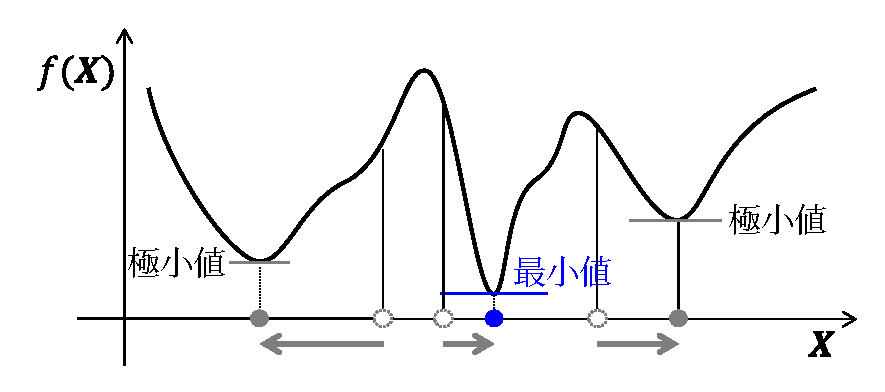
\includegraphics[width=.93\linewidth]{sections/optimization/hill_climbing}
\caption{山登り法(山下り法)による最適解の探索.初期値によっては局所解しか見つからない.}
\label{fig:hill_climbing}
\end{figure}

\subsection{最急降下法}
\label{sec:steepest_descent}

最急降下法 (steepest descent method) はもっとも単純な反復最適化技法で,
コスト関数の勾配方向の逆方向にパラメータを更新します.
本節では,パラメータ$\bm{X}$は,$N$次元ベクトル$\bm{x} = [x_1,\cdots,x_N]^T\in \mathbb{R}^N$であるとします.
このとき,関数$f(\bm{x})$の勾配ベクトル (gradient vector) は
\begin{align}
\nabla f(\bm{x}) = \left[\frac{\partial f(\bm{x})}{\partial x_1},\ldots,\frac{\partial f(\bm{x})}{\partial x_N}\right]^T
\end{align}
で与えられます.このとき,$\nabla f(\bm{x})$は$f(\bm{x})$の等高面,
すなわち,$f(\bm{x})$が一定となるような$N$次元空間内の曲面に対して,
その法線ベクトルを与えます.
このベクトルの向きは,関数の値が増加する方向を示しています.

\begin{algobox}{最急降下法}
\label{algo:steepest}
\begin{algorithmic}[1]
\Require 最小化すべきコスト関数$f(\bm{x}) \in \mathbb{R}$
\State パラメータ$\bm{x} \in \mathbb{R}^N$をランダムに初期化
\While{$\nabla f(\bm{x}) \ne \bm{0}$}
\State 探索ベクトル$d(\bm{x}) = - \nabla f(\bm{x})$を計算
\State ステップ幅$\alpha$を適切に設定
\State $\bm{x} \gets \bm{x} + \alpha d(\bm{x})$
\EndWhile\\
{\bf Return} パラメータ$\bm{x}$
\end{algorithmic}
\end{algobox}

\refalgo{algo:steepest}に,$\bm{x}$を更新するアルゴリズムを示します.
具体的に,$\bm{x} = [x_1,x_2]^T$として$f(\bm{x}) = x_1^2 + x_2^2$の最小化について考えてみます.
このとき,勾配ベクトルは
\begin{align}
 \nabla f(\bm{x}) = [2 x_1, 2 x_2]^T
\end{align}
となるので,ある$\bm{x}$における$\nabla f(\bm{x})$の向きは,原点と$\bm{x}$とを結ぶ方向になります.
この例では,$f(\bm{x})$が一定となる等高線は円であり,
確かに$\nabla f(\bm{x})$は等高線に対する法線ベクトルになっています.
したがって,$\nabla f(\bm{x})$の逆向きの方向が
最も$f(\bm{x})$の値が減少する方向$d(\bm{x})$であるので,
$d(\bm{x})$の方向に沿って$\bm{x}$を「少しずつ」動かせばよいのです.

ここで重要なのは,ステップサイズ$\alpha$の設定です.
$\alpha$を大きくすると,$\bm{x}$は大きく更新されるので,局所解へ早く収束しそうです.
しかし,大きくしすぎると,局所解の周辺をいったりきたりしてしまいます.
そのため,実際には,直線探索を用いて適切な$\alpha$を決定することがよく行われます.
一般には,$\alpha$を少しずつ小さくしていくことが好ましいとされています.

最急降下法は,$f(\bm{x})$が唯一の極小点を持つときには,
停留点($\nabla f(\bm{x}) = 0$となる$\bm{x}$)への大域的な収束性が保証されています.
また,計算量が軽く,実装が簡単ですが,収束が遅いことが欠点です.

\subsection{ニュートン法}
\label{sec:newton}

収束が遅いという最急降下法の欠点を克服する方法として,
ニュートン法 (Newton's method) が知られています.
ニュートン法は,コスト関数$f(\bm{x})$の一次導関数$\nabla f(\bm{x})$だけではなく,
二次導関数$\nabla^2 f(\bm{x})$を利用することで,
探索ベクトル$d(\bm{x})$の計算に工夫を行います.
まず,$f(\bm{x})$に対して,二次のテイラー展開を行うと
\begin{align}
f(\bm{x} + \Delta \bm{x}) 
&\approx f(\bm{x}) + \nabla f(\bm{x})^T \Delta\bm{x}
+ \frac{1}{2} \Delta\bm{x}^T \nabla^2 f(\bm{x}) \Delta\bm{x}
\nonumber\\
&\overset{\mbox{\scriptsize def}}{=} t(\bm{x} + \Delta\bm{x})
\label{eq:fx_taylor}
\end{align}
を得ます.ここで,二次導関数$\nabla^2 f(\bm{x})$は
\begin{align}
\nabla^2 f(\bm{x}) =
  \begin{bmatrix}
    \displaystyle
    \frac{\partial^2 f(\bm{x})}{\partial x_1 \partial x_1} &
    \cdots&
    \displaystyle
    \frac{\partial^2 f(\bm{x})}{\partial x_1 \partial x_N}\\
    \vdots & & \vdots \\
    \displaystyle
    \frac{\partial^2 f(\bm{x})}{\partial x_N \partial x_1} &
    \cdots& 
    \displaystyle \frac{\partial^2 f(\bm{x})}{\partial x_N \partial x_N}    
  \end{bmatrix}
\end{align}
で与えられます.$\nabla^2 f(\bm{x})$は,関数$f(\bm{x})$のヘッセ行列 (Hessian matrix) とよばれ,
しばしば$H(\bm{x})$と表されます.
$f(\bm{x})$が二階連続微分可能であれば,$H(\bm{x})$は対称行列となります.
\refeq{eq:fx_taylor}の二次近似の精度が十分によければ,
$t(\bm{x} + \Delta\bm{x})$を最小化する$\Delta\bm{x}$が,
$f(\bm{x} + \Delta\bm{x})$を最小化する$\Delta\bm{x}$のよい近似になっており,
$\bm{x} \gets \bm{x} + \Delta\bm{x}$と更新すればよいことになります.

覚えておくべき重要な性質として,$\bm{x}$が$f(\bm{x})$の極小点をとるには,
ヘッセ行列$H(\bm{x})$は正定値行列である必要があります(必要十分ではありません).
行列の正定値性とは,固有値が全て正であることを意味し,
スカラの正値性を拡張した概念です.
例えば,$N=1$のとき,$f(\bm{x})$はスカラを入力とする関数となり,
その極小点において,一次導関数の値は負から正に切り替わるので,
二次導関数の値は正をとらなくてはなりません.
$N > 1$のときは,$f(\bm{x})$はベクトルを入力とする関数であり,
二次導関数は行列形式で与えられます.
このとき,極小点において,
スカラの正値性を多次元拡張した性質である半正定値性が成立することになります.

ヘッセ行列$H(\bm{x})$が正定値であるとして,
\refeq{eq:fx_taylor}に対して平方完成を行うと,$\Delta\bm{x}$の二次関数
\begin{align}
t(\bm{x} &+ \Delta\bm{x}) 
= f(\bm{x}) - \frac{1}{2} \nabla f(\bm{x})^T H(\bm{x})^{-1} \nabla f(\bm{x}) 
\nonumber\\
&+ \frac{1}{2} \left(\Delta\bm{x} + H(\bm{x})^{-1} 
\nabla f(\bm{x})\right)^T H(\bm{x}) \left(\Delta\bm{x} + H(\bm{x})^{-1} \nabla f(\bm{x})\right)
\end{align}
を得ます.この二次関数は,
\begin{align}
 \Delta\bm{x} = - H(\bm{x})^{-1} \nabla f(\bm{x})
 \label{eq:xi_h_n}
\end{align}
のとき最小値をとります.
したがって,$\bm{x} \gets \bm{x} - H(\bm{x})^{-1} \nabla f(\bm{x})$とすることで
$f(\bm{x})$を効率的に小さくすることができるはずです.

\begin{algobox}{ニュートン法}
\label{algo:newton}
\begin{algorithmic}[1]
\Require 最小化すべきコスト関数$f(\bm{x}) \in \mathbb{R}$
\State パラメータ$\bm{x} \in \mathbb{R}^N$をランダムに初期化
\While{$\nabla f(\bm{x}) \ne \bm{0}$}
\State 探索ベクトル$d(\bm{x}) = - \left(\nabla^2 f(\bm{x})\right)^{-1} \nabla f(\bm{x})$を計算
\State ステップ幅$\alpha$を適切に設定
\State $\bm{x} \gets \bm{x} + \alpha d(\bm{x})$
\EndWhile\\
{\bf Return} パラメータ$\bm{x}$
\end{algorithmic}
\end{algobox}

\refalgo{algo:newton}に,$\bm{x}$を更新するアルゴリズムを示します.
$f(\bm{x})$が二次関数である場合には,\refeq{eq:fx_taylor}の近似で誤差は生じないため,
\refeq{eq:xi_h_n}のときに$f(\bm{x} + \Delta\bm{x})$は最小値をとり,反復は一回で終了します.
実際には,$f(\bm{x})$は二次関数でない場合が普通であり,
探索ベクトル$d(\bm{x})$の方向に$1$以外のスケールで動かせるようにステップ幅$\alpha$が導入されています.

ニュートン法は収束速度が速いですが,
初期値が局所解に十分に近くないと収束性が保証されません.
ただし,実用上は,$\alpha=1$としても問題なく収束する場合が多いです.
また,特に$N$が大きい場合に問題となりますが,数値的に不安定になりやすく,
ヘッセ行列$H(\bm{x})$が正定値性を満たさなくなったり,
逆行列$H(\bm{x})^{-1}$の計算負荷が大きいといった欠点があります.

\subsection{準ニュートン法}
\label{sec:quasi_newton}

ヘッセ行列$H(\bm{x})$やその逆行列を直接計算しなければならないというニュートン法の欠点を克服するため,
準ニュートン法 (quasi-Newton method) が知られています.
準ニュートン法では,最適化の繰り返し計算の過程で得られる勾配ベクトルにより,
ヘッセ行列$H(\bm{x})$の近似を行います.
まず,(精度はともかく)勾配ベクトルは次式で近似できます.
\begin{align}
 \nabla f(\bm{x} + \Delta\bm{x}) \approx \nabla f(\bm{x}) + H(\bm{x})\Delta\bm{x}
\end{align}
したがって,$H(\bm{x})$の近似値として,セカント方程式 (Secant equation)
\begin{align}
 \nabla f(\bm{x} + \Delta\bm{x}) = \nabla f(\bm{x}) + B(\bm{x})\Delta\bm{x}
\end{align}
を満たすような$B(\bm{x})$を求めればよいことになります.

\begin{algobox}{準ニュートン法}
\label{algo:quasi_newton}
\begin{algorithmic}[1]
\Require 最小化すべきコスト関数$f(\bm{x}) \in \mathbb{R}$
\State パラメータ$\bm{x} \in \mathbb{R}^N$をランダムに初期化
\State 近似ヘッセ行列$B(\bm{x})$を初期化(単位行列など)
\While{$\nabla f(\bm{x}) \ne \bm{0}$}
\State 探索ベクトル$d(\bm{x}) = - B(\bm{x})^{-1} \nabla f(\bm{x})$を計算
\State ステップ幅$\alpha$を適切に設定
\State $\bm{x}$の変化量$\Delta\bm{x} = \alpha d(\bm{x})$を計算
\State $\nabla f(\bm{x})$の変化量$\bm{y} = \nabla f(\bm{x} + \Delta\bm{x}) - \nabla f(\bm{x})$を計算
\State $\bm{x} \gets \bm{x} + \Delta\bm{x}$
\State 近似ヘッセ行列の逆行列$B(\bm{x})^{-1}$を更新
\EndWhile\\
{\bf Return} パラメータ$\bm{x}$
\end{algorithmic}
\end{algobox}

\begin{table}[t]
\centering
\caption{近似ヘッセ行列$B(\bm{x})$の更新}
\label{tab:hessian_update}
\begin{tabular}{l|l}
\hline
手法 & 更新式
\\
\hline
DFP 
&
$\displaystyle B(\bm{x}) \gets \left (I-\frac {\bm{y} \, \Delta\bm{x}^T} {\bm{y}^T \, \Delta\bm{x}} \right ) B(\bm{x}) \left (I-\frac {\Delta\bm{x} \bm{y}^T} {\bm{y}^T \, \Delta\bm{x}} \right )+\frac{\bm{y} \bm{y}^T} {\bm{y}^T \, \Delta\bm{x}}$
\parbox[c][9.5mm][c]{0cm}{}\\
BFGS
&
$\displaystyle B(\bm{x}) \gets B(\bm{x}) + \frac {\bm{y} \bm{y}^T}{\bm{y}^{T} \Delta\bm{x}} - \frac {B(\bm{x}) \Delta\bm{x} (B(\bm{x}) \Delta\bm{x})^T} {\Delta\bm{x}^{T} B(\bm{x}) \, \Delta\bm{x}}$
\parbox[c][9.5mm][c]{0cm}{}\\
SR1
&
$\displaystyle B(\bm{x}) \gets B(\bm{x}) +\frac {(\bm{y}-B(\bm{x}) \, \Delta\bm{x}) (\bm{y}-B(\bm{x}) \, \Delta\bm{x})^T}{(\bm{y}-B(\bm{x}) \, \Delta\bm{x})^T \, \Delta\bm{x}}$
\parbox[c][9.5mm][c]{0cm}{}\\
Broyden
&
$\displaystyle B(\bm{x}) \gets B(\bm{x})+\frac {\bm{y}-B(\bm{x}) \Delta\bm{x}}{\Delta\bm{x}^T \, \Delta\bm{x}} \, \Delta\bm{x}^T$
\parbox[c][9.5mm][c]{0cm}{}\\
\hline
\end{tabular}
\end{table}

\begin{table}[t]
\centering
\caption{近似ヘッセ行列の逆行列$C(\bm{x}) = B(\bm{x})^{-1}$の更新}
\label{tab:inv_hessian_update}
\begin{tabular}{l|l}
\hline
手法 & 更新式
\\
\hline
DFP 
&
$\displaystyle C(\bm{x}) \gets \displaystyle C(\bm{x}) + \frac {\Delta\bm{x} \Delta\bm{x}^T}{\bm{y}^{T} \, \Delta\bm{x}} - \frac {C(\bm{x}) \bm{y} \bm{y}^T C(\bm{x})^T} {\bm{y}^T C(\bm{x}) \bm{y}}$
\parbox[c][9.5mm][c]{0cm}{}\\
BFGS
&
$\displaystyle C(\bm{x}) \gets \left (I-\frac {\bm{y} \Delta\bm{x}^T} {\bm{y}^T \Delta\bm{x}} \right )^T C(\bm{x}) \left (I-\frac { \bm{y} \Delta\bm{x}^T} {\bm{y}^T \Delta\bm{x}} \right )+\frac
{\Delta\bm{x} \Delta\bm{x}^T} {\bm{y}^T \, \Delta\bm{x}}$
\parbox[c][9.5mm][c]{0cm}{}\\
SR1
&
$\displaystyle C(\bm{x}) \gets C(\bm{x})+\frac {(\Delta\bm{x}-C(\bm{x}) \bm{y}) (\Delta\bm{x}-C(\bm{x}) \bm{y})^T}{(\Delta\bm{x}-C(\bm{x}) \bm{y})^T \bm{y}}$
\parbox[c][9.5mm][c]{0cm}{}\\
Broyden
&
$\displaystyle C(\bm{x}) \gets C(\bm{x})+\frac {(\Delta\bm{x}-C(\bm{x}) \bm{y}) \Delta\bm{x}^T C(\bm{x})}{\Delta\bm{x}^T C(\bm{x}) \, \bm{y}}$
\parbox[c][9.5mm][c]{0cm}{}\\
\hline
\end{tabular}
\end{table}

\refalgo{algo:quasi_newton}に,$\bm{x}$を更新するアルゴリズムを示します.
準ニュートン法では,パラメータ$\bm{x}$だけではなく,
近似ヘッセ行列$B(\bm{x})$も反復的に更新されるため,
両者を初期化しておく必要があります.
\reftab{tab:hessian_update}および\reftab{tab:inv_hessian_update}に,
近似ヘッセ行列$B(\bm{x})$あるいはその逆行列$C(\bm{x}) = B(\bm{x})^{-1}$を求めるアルゴリズムを示します.
最初のアルゴリズムであるDFP法は,最近はあまり用いられていません.
現在最も用いられているアルゴリズムは,
BFGS法 (提案者であるBroyden, Fletcher, Goldfarb, Shannoの頭文字から) とSR1法です.
準ニュートン法を大規模問題に応用するため,
記憶制限準ニュートン法 (limited-memory quasi-Newton method) が発表され,
BFGS法の記憶制限版としてL-BFGS法が盛んに利用されています.
SR1法は,ヘッセ行列の更新時に正定値性が保存されないため,
不定値行列に対しても用いることができます.
また,Broyden法は行列が対称行列でなくとも良く,
通常の連立方程式の解を求めるのにも使うことができます.

\subsection{補助関数法}
\label{sec:auxiliary_function}

これまで紹介してきた汎用的な最適化技法とは異なり,
ある条件下において収束性の保証された更新則を導出できる補助関数法 (auxiriary-function-based method) を紹介します.
最急降下法やニュートン法では,通常,最適化が進むにつれて,
ステップ幅$\alpha$を徐々に小さくしていくことがよく行われますが,
収束性を担保しつつ,効率的なスケジューリングを行うことはそれほど簡単ではありません.
補助関数法では,このようなステップ幅の設定が不要で,
経験的には高速に収束することが知られています.

\begin{algobox}{補助関数法}
\label{algo:aux_function}
\begin{algorithmic}[1]
\Require 最小化すべきコスト関数$f(\bm{X}) \in \mathbb{R}$
\State 補助変数$\bm\Theta$を導入して,上限関数$u(\bm{X}, \bm\Theta) \in \mathbb{R}$を設計
\State パラメータ$\bm{X}$をランダムに初期化
\While{$u(\bm{X}, \bm\Theta)$の減少量が大きい}
\State $\bm\Theta \gets \argmin_{\bm\Theta} u(\bm{X}, \bm\Theta)$
\State $\bm{X} \gets \argmin_{\bm{X}} u(\bm{X}, \bm\Theta)$
\EndWhile\\
{\bf Return} パラメータ$\bm{X}$
\end{algorithmic}
\end{algobox}

\refalgo{algo:aux_function}に,$\bm{X}$を更新するアルゴリズムを示します.
ここでは,$\bm{X}$はベクトルに限定せず,任意の形式をとるものとします.
補助関数法では,コスト関数$f(\bm{X})$の上限関数$u(\bm{X}, \bm\Theta)$を設計し,
$\bm{X}$と$\bm\Theta$について交互に$u(\bm{X}, \bm\Theta)$を逐次最小化することで,
間接的に$f(\bm{X})$を逐次最小化します.
ここで,$\bm\Theta$は新たに導入された補助変数で,
$u(\bm{X}, \bm\Theta)$を$\bm\Theta$について最小化すると,
もとの関数$f(\bm{X})$と同じ値をとるようにしておきます.
\begin{align}
f(\bm{X}) = \min_{\bm\Theta} u(\bm{X},\bm\Theta)
\end{align}

このアルゴリズムの収束性についてみてみましょう.
いま,あるステップ$k$における$\bm{X}$および$\bm\Theta$の値を
$\bm{X}^{(k)}$および$\bm\Theta^{(k)}$とすると,
上限関数が満たすべき性質から
\begin{align}
f(\bm{X}^{(k)}) 
&= \min_{\bm\Theta} u(\bm{X}^{(k)},\bm\Theta) = u(\bm{X}^{(k)},\bm\Theta^{(k + 1)})
\nonumber\\
&\ge u(\bm{X}^{(k + 1)},\bm\Theta^{(k + 1)})
\nonumber\\
&\ge u(\bm{X}^{(k + 1)},\bm\Theta^{(k + 2)})
= f(\bm{X}^{(k + 1)})
\end{align}
となります(\reffig{fig:aux_function}).
したがって,$\{f(\bm{X}^{(k)})\}_{k=1}^\infty$は単調非増加 (monotonically non-increasing) となり,
停留点に収束します.

\begin{figure}[t]
\centering
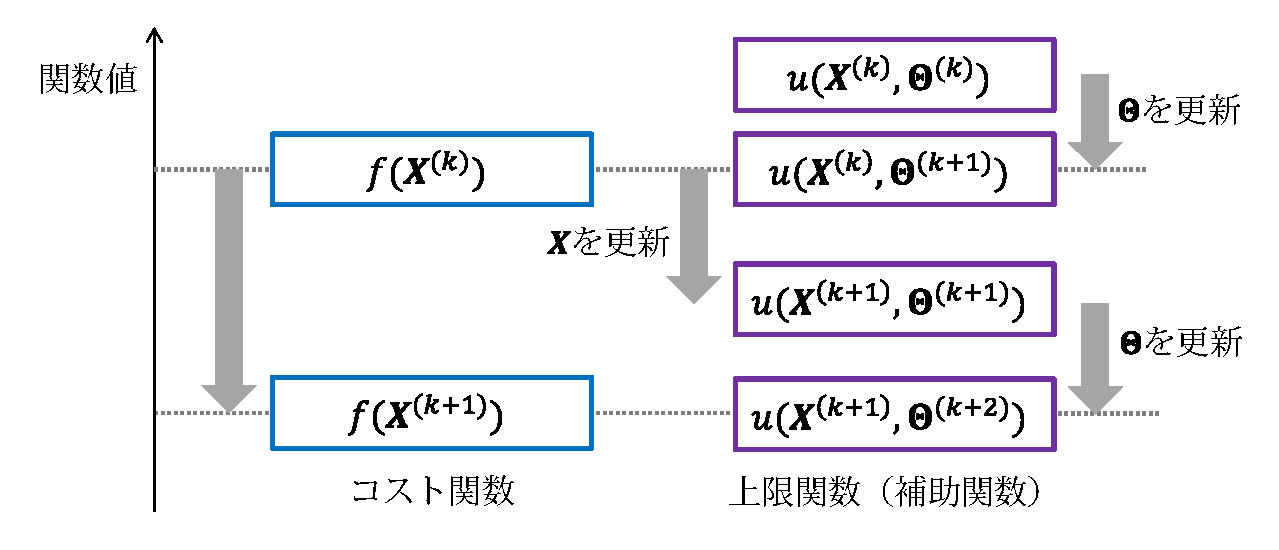
\includegraphics[width=.98\linewidth]{sections/optimization/aux_function}
\vspace{-1mm}
\caption{補助関数法によるパラメータ$\bm{X}$と補助変数$\bm\Theta$の反復最適化.}
\label{fig:aux_function}
\end{figure}

\refsec{sec:opt_model}で説明する確率モデルの最適化においては,
コスト関数を最小化するのではなく,尤度関数を最大化する問題を解く必要があります.
この場合には,尤度関数の符号を反転させることによりコスト関数とみなせて,
補助関数法が適用できる場合があります.

補助関数法の肝は,$f(\bm{X})$を直接最小化する
(例えば$\bm{X}$で偏微分したものをゼロとおいた方程式を解析的に解く)ことが難しい場合に,
一方の変数の値が既知であれば,もう一方の変数について最小化することが容易になるような
$u(\bm{X}, \bm\Theta)$をうまく設計することにあります.
例えば,$u(\bm{X}, \bm\Theta)$が$\bm{X}$に関する凸関数となっており,
$\bm{X}$で偏微分してゼロとおいた式が解析的に解けるとすると,
$\bm\Theta$が与えられたもとでの$\bm{X}$の最適解を得ることができます.
このとき,アルゴリズムは高速に収束することが期待できます.

最適化を行いやすい$u(\bm{X}, \bm\Theta)$を設計するうえで有用な基本原理について説明します.
まず,$f$が凸関数 (convex function) である場合,
イェンセンの不等式 (Jensen's inequality) が適用できる可能性があります.
\begin{theobox}{イェンセンの不等式}
\label{jensen}
任意の凸関数$f:\mathbb{R}^N \mapsto \mathbb{R}$に対して,
\begin{align}
f\left(\sum_{k=1}^K \lambda_k \bm{x}_k\right) \le \sum_{k=1}^K \lambda_k f(\bm{x}_k)
\label{eq:jensen_inequality}
\end{align}
が成立します.
ただし,$\{\bm{x}_k\}_{k=1}^K$は任意の$N$次元ベクトルで,
$\{\lambda_k\}_{k=1}^K$は$\lambda_k \ge 0$かつ$\sum_{k=1}^K \lambda_k = 1$を満たす非負の実数です.
\end{theobox}
これが成立することは,凸関数の定義から明らかです.
\reffig{fig:aux_function_conv_concave}(a)に,
$N=1$のときの様子を示します.
不等式の左辺は,$\{\bm{x}_k\}_{k=1}^K$の重み付き和の関数値を計算していますが,
右辺は,各$\bm{x}_k$における関数値の重み付き和をとっています.
したがって,$f$が凸関数であるならば,後者の方が大きくなります.
例えば,凸関数$f(x) = - \log (x)$に対して,次式が成立します.
\begin{align}
- \log \left(\sum_{k=1}^K \lambda_k x_k\right) \le - \sum_{k=1}^K \lambda_k \log (x_k)
\end{align}

一方,$f$が凹関数 (concave function) である場合,
一次のテイラー展開に基づく接平面を補助関数に用いることができます.
\begin{theobox}{接平面に基づく不等式}
\label{jensen}
任意の凹関数$f:\mathbb{R}^N \mapsto \mathbb{R}$に対して,
\begin{align}
f(\bm{x}) \le f(\bm\omega) + f'(\bm\omega)^T(\bm{x} - \bm\omega)
\end{align}
が成立します.ただし,$\bm{x}$および$\bm\omega$は任意の$N$次元ベクトルです.\\[-4mm]
\end{theobox}
\reffig{fig:aux_function_conv_concave}(b)に,
$N=1$のときの不等式の様子を示します.
不等式の右辺は,$\bm{x}$の一次式であるので,
$N=1$のときは接平面の方程式を表します.
例えば,凹関数$f(x) = \log (x)$に対して,次式が成立します.
\begin{align}
\log(x) \le \log(\omega) + \frac{1}{\omega}(x - \omega) = \frac{x}{\omega} + \log(\omega) - 1
\end{align}

\begin{figure}[t]
\centering
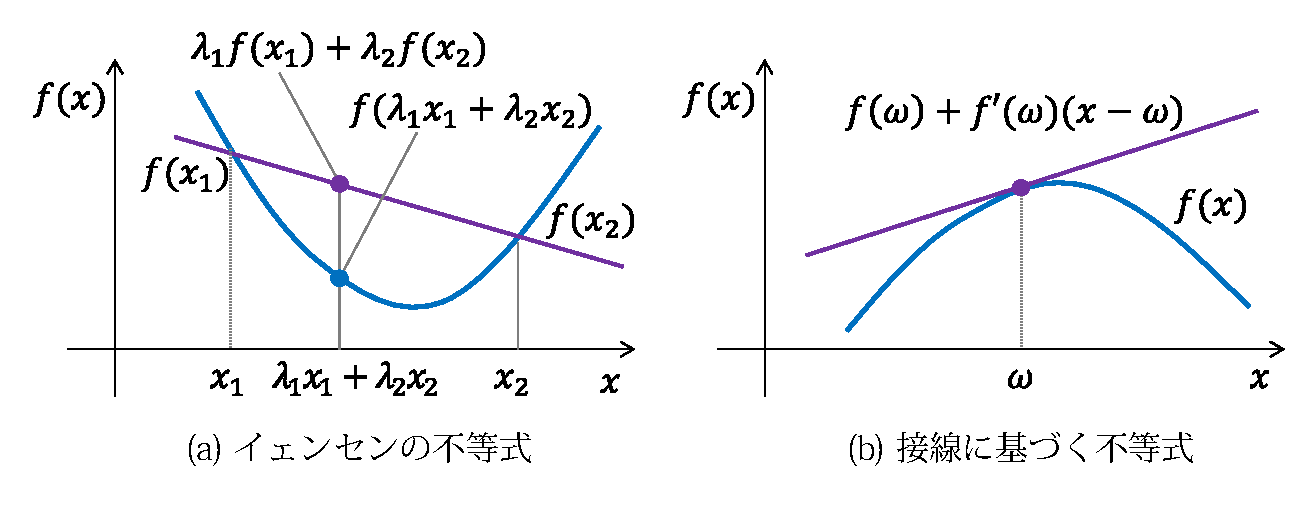
\includegraphics[width=.98\linewidth]{sections/optimization/aux_function_conv_concave}
\vspace{-2mm}
\caption{コスト関数の上限関数を導出するうえで有用な基本原理.}
\label{fig:aux_function_conv_concave}
\end{figure}

\subsection{乗法更新アルゴリズム}
\label{sec:multiplicative_update}

コスト関数$f(\bm{X})$の入力$\bm{X}$が非負値のスカラ$x$である場合には,
乗法更新アルゴリズムと呼ばれる反復最適化技法が利用できる場合があります.
この手法では,特別な制約を導入することなしに,
毎回の反復における$x$の非負値性を自然に保つことができます.

\begin{algobox}{乗法更新アルゴリズム}
\label{algo:multiplicative_update}
\begin{algorithmic}[1]
\Require 最小化すべきコスト関数$f(x) \in \mathbb{R}$
\State パラメータ$x$をランダムに初期化
\While{$f(x)$の減少量が大きい}
\State $\frac{\partial f(x)}{\partial x} = \kappa^+(x) - \kappa^-(x)$を計算.
ただし,$\kappa^+(x) > 0$および$\kappa^-(x) > 0$を満たすものとする.
\State $x \gets \frac{\kappa^-(x)}{\kappa^+(x)} x$
\EndWhile\\
{\bf Return} パラメータ$x$
\end{algorithmic}
\end{algobox}

\refalgo{algo:multiplicative_update}に,乗法更新アルゴリズムを示します.
いま,ある非負の変数$x \ge 0$に関するコスト関数$f(x)$が与えられており,
これを$x$について最小化する問題を考えます.
このとき,$f(x)$の$x$に関する一次導関数が
\begin{align}
\frac{\partial f(x)}{\partial x} = \kappa^+(x) - \kappa^-(x)
\end{align}
の形で表現できたとします.
ただし,$\kappa^+(x) > 0$および$\kappa^-(x) > 0$は
$x$の関数であり,常に正をとるものとします.
このとき,
\begin{align}
x \gets \frac{\kappa^-(x)}{\kappa^+(x)} x
\label{eq:x_mu_update}
\end{align}
とすると,$f(x)$が小さくなることが期待できます.
収束性は理論的に保証されていませんが,
実用上は問題がない場合がほとんどです.

\begin{figure}[t]
\centering
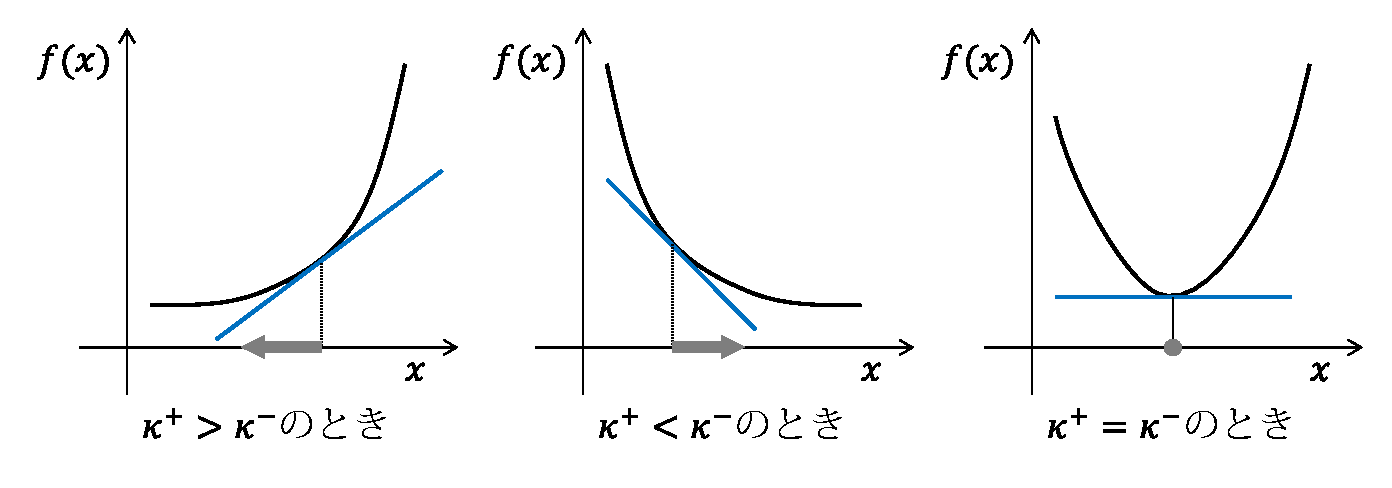
\includegraphics[width=.99\linewidth]{sections/optimization/multiplicative_update}
\caption{$f(x)$の最小化に乗法更新則を適用した場合の$x$の変化.}
\label{fig:multiplicative_update}
\end{figure}

このアルゴリズムが$f(x)$の値をどのように小さくするのかについて,
$\kappa^+$および$\kappa^-$の大小関係で場合分けして考察してみましょう
(\reffig{fig:multiplicative_update}).
\begin{itemize}
\item
$\kappa(x)^+ > \kappa(x)^-$のとき:\\
$\frac{\partial f(x)}{\partial x} > 0$となり,
$f(x)$の$x$に関する傾きは正であるので,
$f(x)$を小さくするには,$x$を小さくする必要があります.
\refeq{eq:x_mu_update}をみると,分子より分母の方が大きくなり,
更新によって$x$が小さくなります.
\item
$\kappa(x)^+ < \kappa(x)^-$のとき:\\
$\frac{\partial f(x)}{\partial x} < 0$となり,
$f(x)$の$x$に関する傾きは負であるので,
$f(x)$を小さくするには,$x$を小さくする必要があります.
\refeq{eq:x_mu_update}をみると,分子より分母の方が小さくなり,
更新によって$x$が大きくなります.
\item
$\kappa(x)^+ = \kappa(x)^-$のとき:\\
$\frac{\partial f(x)}{\partial x} = 0$となり,
$f(x)$は$x$において停留点をとることを示しています.
\refeq{eq:x_mu_update}をみると,
分子と分母が同じになり,$x$は更新されません.
\end{itemize}

\section{確率モデルの最適化}
\label{sec:opt_model}

本節では,確率モデルの学習に必要となる最適化技法について紹介します.
いま,確率モデルのパラメータ(の集合)を$\bm\Theta$,
確率モデルから生成された観測データを$\bm{X}$とします.
観測データ$\bm{X}$が与えられた時に,
確率モデルのパラメータ$\bm\Theta$を推定するには,主に3つのアプローチがあります.
\begin{description}
\item[最尤推定 (maximum-likelihood (ML) estimation)] \ \\
最尤推定では,観測データ$\bm{X}$に対して,
パラメータ$\bm\Theta$の尤度関数 (likelihood function)
$f(\bm\Theta) = p(\bm{X}|\bm\Theta)$を
最大化するような$\bm\Theta^*$を点推定する(一意に決定する)ことが目標です.
\begin{align}
\bm\Theta^* = \argmax_{\bm\Theta} p(\bm{X}|\bm\Theta)
\end{align}
ここで,$p(\bm{X}|\bm\Theta)$は,$\bm\Theta$から$\bm{X}$が生成される
確率\footnote{連続側の分布の場合,正確には確率密度ですが,
本書では区別せずに「確率」と呼びます.
また,パラメータ$\bm\Theta$を確率変数として取り扱わない場合は,
$p(\bm{X} | \bm\Theta)$ではなく$p(\bm{X} ; \bm\Theta)$として表記する場合も多いです.
本書では,これらの区別は特に行いません.}を表すので,
この値が大きい$\bm\Theta$ほど尤もらしいと考え,
$p(\bm{X}|\bm\Theta)$を$\bm\Theta$の良さを評価する関数$f(\bm\Theta)$であるとみなします.
この尤度関数はコスト関数の符号を反転したものであるとみなすことで,
最適解が解析的に求められない場合は,
これまで説明してきた反復最適化技法を利用することができます.
最尤推定は幅広く用いられている最も基本的なアプローチですが,
観測データ$\bm{X}$があまり大きくない場合には,
推定結果が不正確になりやすい問題があります.
なぜなら,パラメータの値は観測データ$\bm{X}$のみで決まり,
何らかの制約を加えることができないからです.

\item[最大事後確率推定 (maximum-a-posteriori (MAP) estimation)] \ \\
MAP推定では,パラメータ$\bm\Theta$に対する事前分布$p(\bm\Theta)$を導入し,
事前分布$p(\bm\Theta)$と尤度関数$p(\bm{X}|\bm\Theta)$との積を
最大化するような$\bm\Theta^*$を点推定することが目標です.
\begin{align}
\bm\Theta^* = \argmax_{\bm\Theta} p(\bm{X}|\bm\Theta) p(\bm\Theta)
\end{align}
ただし,MAP推定では,事前知識を反映して,$p(\bm\Theta)$を適切に設定する必要があります.
もし,$\bm\Theta$がさまざまな値を取りうる可能性が高い場合はなだらかな確率分布を,
$\bm\Theta$がある特定の値の近くを取ることが分かっている場合は急峻な確率分布を設定します.
これにより,事前知識\footnote{「仮想的な」観測データと解釈することができます.
多くの場合,$p(\bm\Theta)$には仮想的な観測データの個数と解釈できるパラメータが含まれており,
パラメータ推定時に事前分布をどの程度重視するかを自由に制御することができます.}と
実際の観測データとを考慮することで,
観測データが小さい場合でも,事前知識に基づく安定したパラメータ推定が可能になります.
事前分布が一様分布の場合(事前知識が特にない場合),MAP推定は最尤推定と同じ結果を与えます.
MAP推定においても,最尤推定と同様に,標準的な方法を用いた最適化が可能です.

\item[ベイズ推定 (Bayesian estimation)] \ \\
最尤推定・MAP推定では,パラメータ$\bm\Theta$を点推定していたのに対し,
ベイズ推定では,ベイズの定理を用いることで,
事前分布$p(\bm\Theta)$と尤度関数$p(\bm{X}|\bm\Theta)$から
事後分布$p(\bm\Theta|\bm{X})$を求めることが目標です.
\begin{align}
 p(\bm\Theta|\bm{X}) 
 = \frac{p(\bm{X}|\bm\Theta)p(\bm\Theta)}{p(\bm{X})}
 = \frac{p(\bm{X}|\bm\Theta)p(\bm\Theta)}{\int p(\bm{X}|\bm\Theta) p(\bm\Theta) d\bm\Theta}
 \label{eq:bayes_theorem}
\end{align}
本来,$\bm\Theta$は未知ですから,その推定結果には不確実性が伴います.
したがって,観測データが十分にない場合には,
100\%の確信度をもって$\bm\Theta$の値を一意に決めることは難しく,
$\bm\Theta$のあらゆる可能性を考慮しておくことが望ましいでしょう.
ベイズ推定では,$\bm\Theta$の取りうる値それぞれについて,
それがどの程度尤もらしいかという確信度,すなわち確率値を計算します.
観測データが増加するにつれて,事後分布は急峻になり,
観測データが無限にある場合は,最尤推定で求まる$\bm\Theta^*$に収束します.

現実の多くの問題においては,\refeq{eq:bayes_theorem}の分母,
すなわち周辺尤度$p(\bm{X})$を求める際の積分計算を解析的に実行することは困難なため,
真の事後分布$p(\bm\Theta|\bm{X})$を正確に求めることは容易ではありません.
主な近似推論方法として,\secref{sec:vb}で説明する変分ベイズ法 (variational Bayesian (VB) methods) と
\secref{sec:mcmc}で説明する
%マルコフ連鎖モンテカルロ法 (Markov chain Monte Carlo (MCMC) methods) の一種である
ギブスサンプリング (Gibbs sampling) が知られており,
いずれも反復計算を行うことで,事後分布$p(\bm\Theta|\bm{X})$を近似する最適化技法です.
\end{description}

\subsection{潜在変数モデル}

\begin{figure}[t]
\centering
\begin{minipage}{.355\linewidth}
\centering
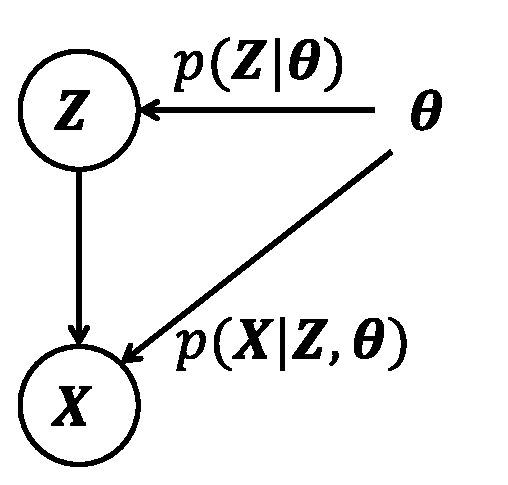
\includegraphics[width=.99\linewidth]{sections/optimization/model_ml}
\caption{最尤推定のための確率モデル.}
\label{fig:model_ml}
\end{minipage}
\hspace{6pt}
\begin{minipage}{.56\linewidth}
\centering
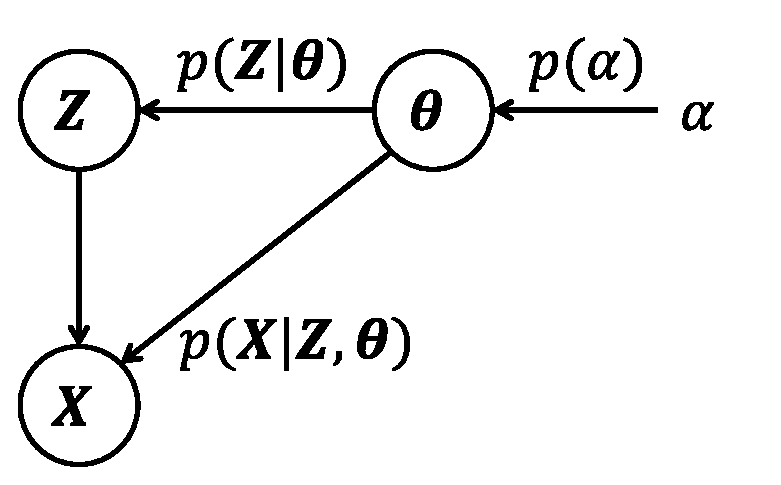
\includegraphics[width=.99\linewidth]{sections/optimization/model_bayes}
\caption{事前分布を導入したベイズモデル.}
\label{fig:model_bayes}
\end{minipage}
\end{figure}

現実の多くの問題においては,潜在変数モデル (latent variable models) と呼ばれる
確率モデルを用いる必要があります.
潜在変数モデルでは,パラメータ$\bm\Theta$に加えて,
観測変数 (observable variables) $\bm{X}$の背後に潜在変数 (latent variables) $\bm{Z}$を考えます.
\begin{align}
p(\bm{X},\bm{Z}|\bm\Theta) = p(\bm{X}|\bm{Z},\bm\Theta) p(\bm{Z} | \bm\Theta)
\end{align}
つまり,観測変数はパラメータから直接生成されるのではなく,
何らかの潜在変数に影響を受けて生成されると考えます.
潜在変数モデルに対して,パラメータの最尤推定を行う場合には,最適化問題
\begin{align}
\bm\Theta^* = \argmax_{\bm\Theta} p(\bm{X}|\bm\Theta) = \argmax_{\bm\Theta} \int p(\bm{X},\bm{Z}|\bm\Theta) d\bm{Z}
\label{eq:model_ml}
\end{align}
を解くことになります.
ここで,潜在変数$\bm{Z}$は確率変数ですが,
パラメータ$\bm\Theta$は確率変数ではないことに注意してください.

本来,パラメータ$\bm\Theta$は潜在変数$\bm{Z}$同様に未知であるので,
不確実性を取り扱う,すなわち,確率変数として取り扱う方が望ましいでしょう.
このとき,パラメータ$\bm\Theta$に対する事前分布$p(\bm\Theta)$を導入することで,ベイズモデル
\begin{align}
p(\bm{X},\bm{Z},\bm\Theta) = p(\bm{X}|\bm{Z},\bm\Theta) p(\bm{Z} | \bm\Theta) p(\bm\Theta)
\end{align}
を定式化することができます.
このモデルに対してベイズ推定を行う場合には,ベイズの定理を用いて,
パラメータ$\bm\Theta$と潜在変数$\bm{Z}$の事後分布を求めることになります.
\begin{align}
 p(\bm{Z},\bm\Theta|\bm{X}) 
 &= \frac{p(\bm{X}|\bm{Z},\bm\Theta) p(\bm{Z} | \bm\Theta) p(\bm\Theta)}{p(\bm{X})}
 \nonumber\\
 &= \frac{p(\bm{X}|\bm{Z},\bm\Theta) p(\bm{Z} | \bm\Theta) p(\bm\Theta)}
 {\int\int p(\bm{X}|\bm{Z},\bm\Theta) p(\bm{Z} | \bm\Theta) p(\bm\Theta)d\bm{Z}d\bm\Theta}
\label{eq:model_bayes}
\end{align}
現実には,
\refeq{eq:model_bayes}の分母の積分を解析的に計算することはできないことがほとんどなので,
あとで説明する近似アルゴリズムが必要になります.

\subsection{最尤推定:EMアルゴリズム}
\label{sec:em}

潜在変数モデルに対して最尤推定を行うための決定論的 (deterministic) な手法が
Expectation-Maximization (EM) アルゴリズムです.
実は,EMアルゴリズムは
\refsec{sec:auxiliary_function}で説明した補助関数法の一種です.
\reffig{fig:em_update}に示すように,
\refeq{eq:model_ml}において,尤度関数$p(\bm{X}|\bm\Theta)$を
直接最大化することは困難なので,その下限関数を最大化することで,
間接的に$p(\bm{X}|\bm\Theta)$を最大化することを考えます.
いま,潜在変数$\bm{Z}$に関する任意の分布$q(\bm{Z})$を考えて,
対数尤度関数$\log p(\bm{X}|\bm\Theta)$の下限関数$\mathcal{L}(q(\bm{Z}),\bm\Theta)$を設計します.
\begin{align}
 \log p(\bm{X}|\bm\Theta)
&= \log \int p(\bm{X},\bm{Z}|\bm\Theta) d\bm{Z}
 \nonumber\\
&= \log \int q(\bm{Z}) 
 \frac{p(\bm{X},\bm{Z}|\bm\Theta)}{q(\bm{Z})} d\bm{Z}
 \nonumber\\
&
 \ge \int q(\bm{Z})
 \log \frac{p(\bm{X},\bm{Z}|\bm\Theta)}{q(\bm{Z})} d\bm{Z}
 \nonumber\\
&
 = \mathbb{E}_{q(\bm{Z})}[\log p(\bm{X},\bm{Z}|\bm\Theta)]
 - \mathbb{E}_{q(\bm{Z})}[\log q(\bm{Z})]
 \nonumber\\
&
 \overset{\mbox{\scriptsize def}}{=} \mathcal{L}(q(\bm{Z}),\bm\Theta)
\label{eq:em_lower_bound}
\end{align}
ここで,対数関数が凹関数であることから,
\refeq{eq:jensen_inequality}で与えられるイェンセンの不等式を用いることで,
和の対数を対数の和に変換しました.
$\mathcal{L}(q(\bm{Z}),\bm\Theta)$は,Q関数 (Q-function) と呼ばれ,
パラメータ$\bm\Theta$の関数であると同時に,
関数$q(\bm{Z})$の汎関数 (functional) となっています.
EMアルゴリズムは,Expectation (E) ステップで補助関数$q(\bm{Z})$に関する最適化を,
Maximization (M) ステップでパラメータ$\bm\Theta$に関する最適化を行い,
これらを交互に反復します.
この手順で,$\mathcal{L}(q(\bm{Z}),\bm\Theta)$は単調非減少 (monotonically non-decreasing)
となり,収束性が保障されます.

\begin{figure}[t]
\centering
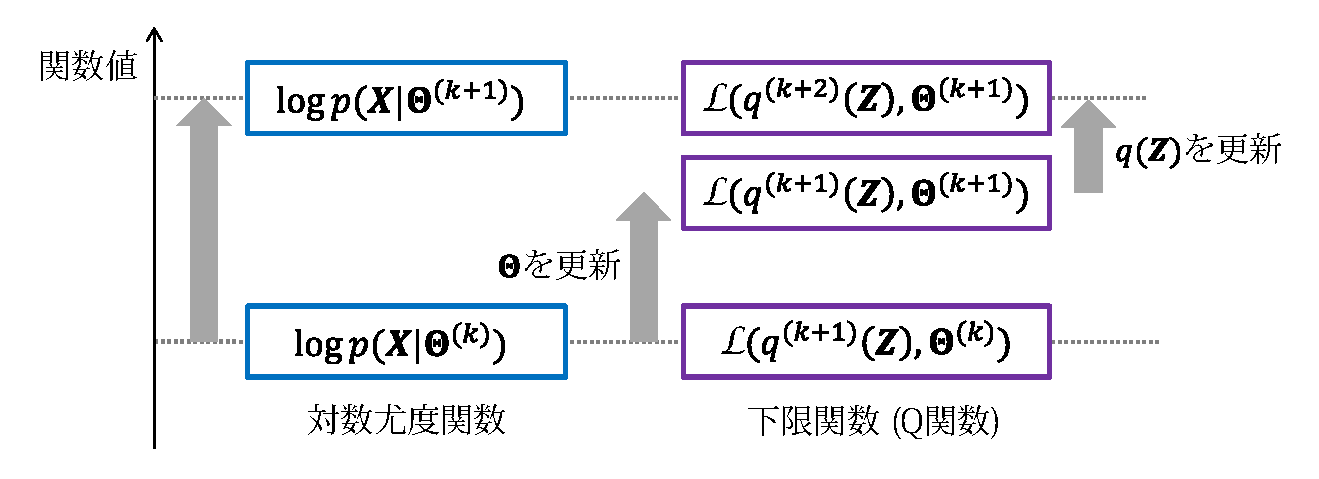
\includegraphics[width=.98\linewidth]{sections/optimization/em_update}
\vspace{-1mm}
\caption{EMアルゴリズムによるパラメータ$\bm{X}$と補助関数$q(\bm\Theta)$の反復最適化.}
\label{fig:em_update}
\end{figure}

まず,Eステップにおいては,パラメータ$\bm\Theta$が既知のもとで,
\refeq{eq:em_lower_bound}において等号が成立する,
すなわち,$\mathcal{L}(q(\bm{Z}),\bm\Theta)$を最大化する$q(\bm{Z})$を求めることが目的です.
これは,制約条件
\begin{align}
\int q(\bm{Z}) d\bm{Z} = 1
\label{eq:qz_1}
\end{align}
付きの最大化問題なので,
ラグランジュの未定乗数法を用いて解くことができます.
まず,未定乗数$\lambda$を導入した関数
\begin{align}
F(q(\bm{Z}))
 = \int q(\bm{Z}) \log \frac{p(\bm{X},\bm{Z}|\bm\Theta)}{q(\bm{Z})} d\bm{Z}
 + \lambda \left(1 - \int q(\bm{Z}) d\bm{Z}\right)
\end{align}
を考えます.
これを$q(\bm{Z})$で偏微分してゼロとおくと,
\begin{align}
\frac{\partial F(q(\bm{Z}))}{\partial q(\bm{Z})}
= \log p(\bm{X},\bm{Z}|\bm\Theta) - \log q(\bm{Z}) - 1 - \lambda = 0
\end{align}
を得ます.これを解くと,
\begin{align}
q(\bm{Z}) = e^{- 1 - \lambda} p(\bm{X},\bm{Z}|\bm\Theta)
\label{eq:qz}
\end{align}
となるので,これを\refeq{eq:qz_1}に代入すると,
\begin{align}
e^{- 1 - \lambda} \int p(\bm{X},\bm{Z}|\bm\Theta) d\bm{Z} = 1
\end{align}
となり,未定乗数$\lambda$は
\begin{align}
e^{- 1 - \lambda} = \frac{1}{\int p(\bm{X},\bm{Z}|\bm\Theta) d\bm{Z}}
\label{eq:lambda}
\end{align}
で与えられます.
最終的に,\refeq{eq:lambda}を\refeq{eq:qz}に代入すると,
最適な$q(\bm{Z})$を求めることができます.
\begin{align}
q(\bm{Z})
= \frac{p(\bm{X},\bm{Z}|\bm\Theta)}{\int p(\bm{X},\bm{Z}|\bm\Theta) d\bm{Z}}
= \frac{p(\bm{X},\bm{Z}|\bm\Theta)}{p(\bm{X}|\bm\Theta)}
= p(\bm{Z}|\bm{X},\bm\Theta)
\label{eq:p_z_x_theta}
\end{align}

次に,Mステップでは,$q(\bm{Z})$が既知のもとで,
$\mathcal{L}(q(\bm{Z}),\bm\Theta)$を最大化する$\bm\Theta$を求めます.
\refeq{eq:em_lower_bound}において,
%Eステップで最適化された$q(\bm{Z})$は定数とみなせるので,
%$\mathbb{E}_{q(\bm{Z})}[\log q(\bm{Z})]$は定数になるので,
$\mathbb{E}_{q(\bm{Z})}[\log p(\bm{X},\bm{Z}|\bm\Theta)]$(一般にQ関数と呼ばれています)の
最大化を考えればよいことになります.
基本的には,$\bm\Theta$で偏微分してゼロとおくことで,
$\bm\Theta$の更新式が得られます.

\begin{algobox}{EMアルゴリズム}
\label{algo:em}
\begin{algorithmic}[1]
\Require 潜在変数モデル$p(\bm{X},\bm{Z}|\bm\Theta) = p(\bm{X}|\bm{Z},\bm\Theta) p(\bm{Z} | \bm\Theta)$
\State 分布$q(\bm{Z})$およびパラメータ$\bm\Theta$をランダムに初期化
\While{$\mathcal{L}(q(\bm{Z}),\bm\Theta)$が収束していない}
\State Eステップ:$q(\bm{Z}) = p(\bm{Z}|\bm{X},\bm\Theta)$
\State Mステップ:$\bm\Theta \leftarrow \argmax_{\bm\Theta} \mathbb{E}_{q(\bm{Z})}[\log p(\bm{X},\bm{Z}|\bm\Theta)]$
\EndWhile\\
{\bf Return} 分布$q(\bm{Z})$およびパラメータ$\bm\Theta$
\end{algorithmic}
\end{algobox}

\refalgo{algo:em}にEMアルゴリズムの手順を示します.
EMアルゴリズムでは,Eステップで$q(\bm{Z})$を潜在変数$\bm{Z}$の事後分布と一致させることで,
下限関数$\mathcal{L}(q(\bm{Z}),\bm\Theta)$が対数尤度関数$\log p(\bm{X}|\bm\Theta)$に等しくなり,
Mステップでパラメータ$\bm\Theta$を最適化することで,対数尤度関数$\log p(\bm{X}|\bm\Theta)$が増加します.
このように,直接$\log p(\bm{X}|\bm\Theta)$を増加させることは難しいものの,
Eステップをはさむことで最適化を容易にする補助関数法となっています.

\subsection{ベイズ推定:変分ベイズ法}
\label{sec:vb}

潜在変数モデルに対してベイズ推定を行うための決定論的な手法が
変分ベイズ法 (variational Bayesian method, VB) です.
一般に,\refeq{eq:model_bayes}において,真の事後分布$p(\bm{Z},\bm\Theta|\bm{X})$を
解析的に計算することは困難です.
VBでは,因子分解可能な変分事後分布$q(\bm{Z},\bm\Theta)=q(\bm{Z})q(\bm\Theta)$を考え,
真の事後分布$p(\bm{Z},\bm\Theta|\bm{X})$にできる限り近づけるような最適化を行います.
したがって,最終的に求まる$q(\bm{Z},\bm\Theta)$は
真の事後分布$p(\bm{Z},\bm\Theta|\bm{X})$には一致せず,
あくまで事後分布の近似計算手法であることに注意が必要です.

ベイズ推定の難しさは,\refeq{eq:model_bayes}の分母である
周辺尤度 (marginal likelihood) あるいはエビデンス (evidence) $p(\bm{X})$の
解析的な計算が困難な点にあります.
したがって,$p(\bm{X})$を精度良く近似できれば,
事後分布$p(\bm{Z},\bm\Theta|\bm{X})$を精度良く近似することができます.
EMアルゴリズムと同様,VBも\refsec{sec:auxiliary_function}で説明した補助関数法の一種となっており,
対数周辺尤度$\log p(\bm{X})$の下限関数を設計し,
それを最大化することにより,$\log p(\bm{X})$のよい近似値を求めます.
下限関数は以下の通り導出できます.
\begin{align}
 \log p(\bm{X})
&= \log \int\int p(\bm{X},\bm{Z},\bm\Theta) d\bm{Z}d\bm\Theta
 \nonumber\\
&= \log \int\int q(\bm{Z},\bm\Theta)
 \frac{p(\bm{X},\bm{Z},\bm\Theta)}{q(\bm{Z},\bm\Theta)} d\bm{Z}d\bm\Theta
 \nonumber\\
&
 \ge \int\int q(\bm{Z},\bm\Theta)
 \log \frac{p(\bm{X},\bm{Z},\bm\Theta)}{q(\bm{Z},\bm\Theta)} d\bm{Z}d\bm\Theta
 \nonumber\\
&
 = \int\int q(\bm{Z})q(\bm\Theta)
 \log \frac{p(\bm{X},\bm{Z},\bm\Theta)}{q(\bm{Z})q(\bm\Theta)} d\bm{Z}d\bm\Theta
 \nonumber\\
&
 = \mathbb{E}_{q(\bm{Z})q(\bm\Theta)}[\log p(\bm{X},\bm{Z},\bm\Theta)]
 - \mathbb{E}_{q(\bm{Z})}[\log q(\bm{Z})]
 - \mathbb{E}_{q(\bm\Theta)}[\log q(\bm\Theta)]
 \nonumber\\
&
 \overset{\mbox{\scriptsize def}}{=} \mathcal{L}(q(\bm{Z}),q(\bm\Theta))
\label{eq:vb_lower_bound}
\end{align}
ここで,対数関数が凹関数なので,
\refeq{eq:jensen_inequality}で与えられるイェンセンの不等式を用いました.
$\mathcal{L}(q(\bm{Z}),q(\bm\Theta))$は,
変分下限 (variational lower bound) あるいは
エビデンス下限 (evidence lower bound, ELBO) と呼ばれ,
関数$q(\bm{Z})$および$q(\bm\Theta)$の汎関数です.
\reffig{fig:vb_update}に示す通り,
VBでは,VB-Eステップで$q(\bm{Z})$に関する最適化を,
VB-Mステップで$q(\bm\Theta)$に関する最適化を行い,
これらを交互に反復します.
このように,汎関数を最大化する関数を求める問題を解くことから,
VBは変分法の一種となっています.

\begin{figure}[t]
\centering
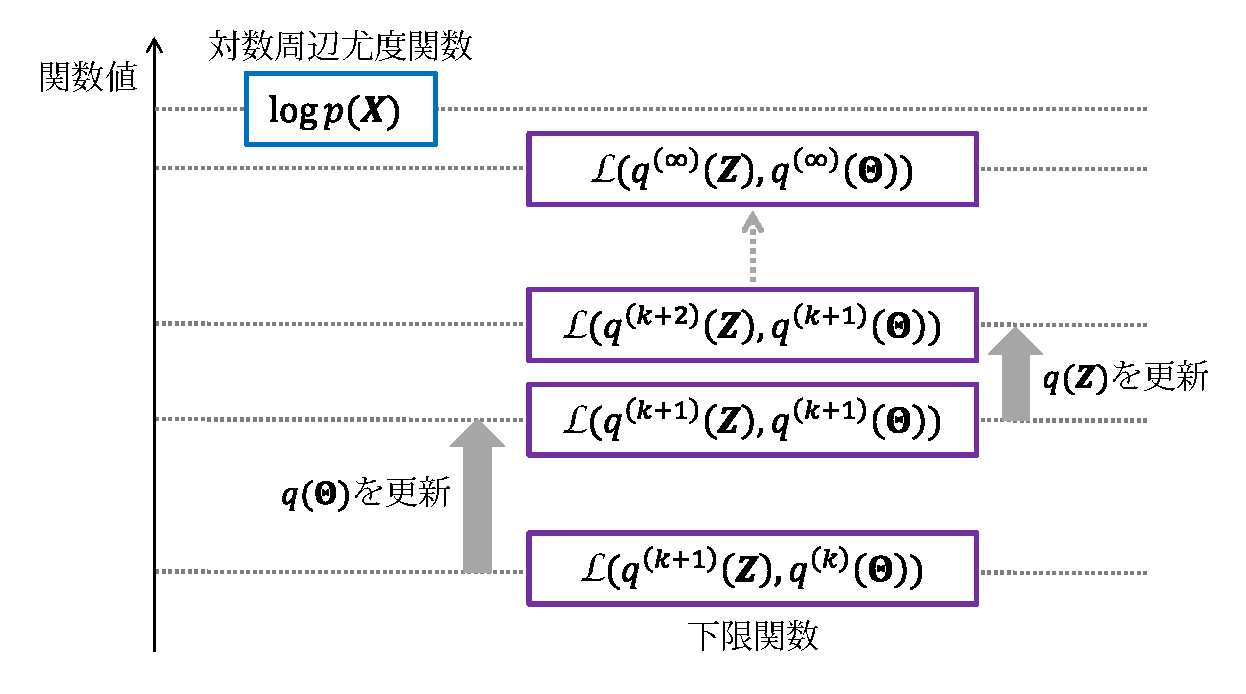
\includegraphics[width=.94\linewidth]{sections/optimization/vb_update}
\vspace{-2mm}
\caption{変分ベイズ法による補助関数$q(\bm{Z})$および$q(\bm\Theta)$の反復最適化.}
\label{fig:vb_update}
\end{figure}

EMアルゴリズムにおいて,
\refeq{eq:em_lower_bound}の等号成立条件は\refeq{eq:p_z_x_theta}であるのと同様,
VBにおいても,\refeq{eq:vb_lower_bound}の等号成立条件は,
\begin{align}
 q(\bm{Z},\bm\Theta) = p(\bm{Z},\bm\Theta|\bm{X})
 \label{eq:vb_equality_condition}
\end{align}
すなわち,$q(\bm{Z},\bm\Theta)$が真の事後分布$p(\bm{Z},\bm\Theta|\bm{X})$と等しいときです.
しかし,$p(\bm{Z},\bm\Theta|\bm{X})$を解析的に計算することは困難です.
そこで,本来,$\bm{Z}$と$\bm\Theta$は独立ではないので,
$p(\bm{Z},\bm\Theta|\bm{X}) = p(\bm{Z}|\bm{X}) p(\bm\Theta|\bm{X})$は成立しませんが,
VBでは,$q(\bm{Z},\bm\Theta) = q(\bm{Z})q(\bm\Theta)$という因数分解ができるという強い仮定を置きます.
この結果,\refeq{eq:vb_lower_bound}の等号は成立しなくなりますが,
$\mathcal{L}(q(\bm{Z}),q(\bm\Theta))$を
$q(\bm\Theta)$および$q(\bm{Z})$について最大化することで,
$\log p(\bm{X})$をできる限り正確に近似できる
$q(\bm\Theta)$および$q(\bm{Z})$を探す問題を解くことを考えます.

因数分解の仮定$q(\bm{Z},\bm\Theta) = q(\bm{Z})q(\bm\Theta)$によって
引き起こされる近似誤差を評価するため,
\refeq{eq:vb_lower_bound}の左辺から右辺を引いた差分を計算してみます.
\begin{align}
&\log p(\bm{X})
-
\int\int q(\bm{Z},\bm\Theta)
 \log \frac{p(\bm{X},\bm{Z},\bm\Theta)}{q(\bm{Z},\bm\Theta)} d\bm{Z}d\bm\Theta
\nonumber\\
&=
\int\int q(\bm{Z},\bm\Theta) \log p(\bm{X}) d\bm{Z}d\bm\Theta
-
\int\int q(\bm{Z},\bm\Theta)
 \log \frac{p(\bm{X},\bm{Z},\bm\Theta)}{q(\bm{Z},\bm\Theta)} d\bm{Z}d\bm\Theta
\nonumber\\
&=
\int\int q(\bm{Z},\bm\Theta)
 \log \frac{q(\bm{Z},\bm\Theta)}{p(\bm{Z},\bm\Theta|\bm{X})} d\bm{Z}d\bm\Theta
\nonumber\\
&=
\mbox{KL}(q(\bm{Z},\bm\Theta) \Vert p(\bm{Z},\bm\Theta|\bm{X}))
\end{align}
ここで,$\mbox{KL}(q \Vert p)$は確率分布$q$の確率分布$p$に対する
カルバック・ライブラーダイバージェンス (Kullback-Leibler (KL) divergence) で,
必ず非負値をとり,$q=p$となるときに限り,最小値の0をとります.
したがって,$q(\bm{Z},\bm\Theta) = p(\bm{Z},\bm\Theta|\bm{X})$であれば,
\refeq{eq:vb_lower_bound}の等号が成立しますが,
$q(\bm{Z},\bm\Theta) = q(\bm{Z})q(\bm\Theta)$を仮定した場合には,近似誤差が生じます.
したがって,VBは,真の事後分布$p(\bm{Z},\bm\Theta|\bm{X})$に対するKL情報量を最小化する
変分事後分布$q(\bm{Z})q(\bm\Theta)$を計算する問題を解いていることになります.

まず,VB-Eステップにおいて,$q(\bm\Theta)$が既知のもとで,
\refeq{eq:vb_lower_bound}における
$\mathcal{L}(q(\bm{Z}),q(\bm\Theta))$を最大化する$q(\bm{Z})$を求めます.
これは,制約条件
\begin{align}
\int q(\bm{Z}) d\bm{Z} = 1
\end{align}
付きの最大化問題なので,
EMアルゴリズムと同様に,ラグランジュの未定乗数法を用いて解くことができます.
%まず,未定乗数$\lambda$を導入した関数
%\begin{align}
%F(q(\bm{Z}))
% = \int q(\bm{Z})q(\bm\Theta) \log \frac{p(\bm{X},\bm{Z},\bm\Theta)}{q(\bm{Z})q(\bm\Theta)} d\bm{Z}d\bm\Theta
% + \lambda \left(1 - \int q(\bm{Z}) d\bm{Z}\right)
%\end{align}
%を考えます.
%これを$q(\bm{Z})$で偏微分してゼロとおくと,
最終的に
\begin{align}
q(\bm{Z}) 
\propto \exp\left(\mathbb{E}_{q(\bm\Theta)}[\log p(\bm{X},\bm{Z},\bm\Theta)]\right)
\end{align}
を得ます.
VB-Mステップにおいては,$q(\bm{Z})$が既知のもとで,
\refeq{eq:vb_lower_bound}における
$\mathcal{L}(q(\bm{Z}),q(\bm\Theta))$を最大化する$q(\bm\Theta)$を求めます.
VB-Eステップとは$\bm{Z}$と$\bm\Theta$の役割が入れ替わっただけなので,
同様に導出できて,
\begin{align}
q(\bm\Theta) 
\propto \exp\left(\mathbb{E}_{q(\bm{Z})}[\log p(\bm{X},\bm{Z},\bm\Theta)]\right)
\end{align}
を得ます.
このように,VBでは,潜在変数とパラメータを区別することなく,
いずれも確率変数として対等に取り扱うことができます.

\begin{algobox}{変分ベイズ法}
\label{algo:vb}
\begin{algorithmic}[1]
\Require ベイズモデル$p(\bm{X},\bm{Z},\bm\Theta) = p(\bm{X}|\bm{Z},\bm\Theta) p(\bm{Z} | \bm\Theta) p(\bm\Theta)$
\State 分布$q(\bm{Z})$および$q(\bm\Theta)$をランダムに初期化
\While{$\mathcal{L}(q(\bm{Z}),q(\bm\Theta))$が収束していない}
\State VB-Eステップ:$q(\bm{Z}) \propto \exp\left(\mathbb{E}_{q(\bm\Theta)}[\log p(\bm{X},\bm{Z},\bm\Theta)]\right)$
\State VB-Mステップ:$q(\bm\Theta) \propto \exp\left(\mathbb{E}_{q(\bm{Z})}[\log p(\bm{X},\bm{Z},\bm\Theta)]\right)$
\EndWhile\\
{\bf Return} 分布$q(\bm{Z})$および$q(\bm\Theta)$
\end{algorithmic}
\end{algobox}

\newpage

\refalgo{algo:vb}にVBを示します.
EMアルゴリズム(\refalgo{algo:em})とVB(\refalgo{algo:vb})を比較すると,
Eステップでは潜在変数の事後分布を計算する点で共通していますが,
Mステップでは,EMアルゴリズムではパラメータを点推定しているのに対し,
VBではパラメータの事後分布を計算している点で異なります.
VBはいずれのステップにおいても,確率変数の期待値を計算していることから,
本来はExpectation-Expectation (EE) アルゴリズムと呼ぶべきものであることが分かります.

より一般に,あるベイズモデル$p(\bm{X},\bm\Theta)=p(\bm{X}|\bm\Theta)p(\bm\Theta)$を
構成する確率変数$\bm\Theta$(パラメータや潜在変数の区別を問わない)が,
$M$個のグループ$\{\bm\Theta_1,\cdots,\bm\Theta_M\}$に分けられる場合について考えます.
このとき,VBでは,変分事後分布$q(\bm\Theta)$を因子分解できる形
$q(\bm\Theta) = \prod_{m=1}^M q(\bm\Theta_m)$に限定して,
その中で,$p(\bm\Theta|\bm{X})$に対するKLダイバージェンスが最小となるものを探します.
このときの各グループの変分事後分布の更新則は,
\begin{align}
q(\bm\Theta_m) 
\propto 
\exp\left(
\mathbb{E}_{q(\bm\Theta_{\neg m})}
\left[\log p(\bm{X},\bm\Theta)\right]
\right)
\end{align}
で与えられます.
ここで,$\neg m$は$m$を除いた全てのインデクスを表すものとし,
$q(\bm\Theta_{\neg m}) = q(\bm\Theta_1) \cdots q(\bm\Theta_{m-1}) q(\bm\Theta_{m+1}) \cdots q(\bm\Theta_M)$です.
確率変数$\bm\Theta$をどのように分割するかが重要で,この分割数$M$が少ないほど,
独立性の仮定が弱くなるので,$q(\bm\Theta)$の$p(\bm\Theta|\bm{X})$に対する近似精度がよくなります.

\subsection{ベイズ推定:ギブスサンプリング}
\label{sec:mcmc}

ギブスサンプリング (Gibbs sampling) は
マルコフ連鎖モンテカルロ法 (Markov chain Monte Carlo methods, MCMC) の一種で,
任意の確率分布に従うサンプルをランダムに生成することができる汎用的な方法です.
ベイズ推定の難しさは,\refeq{eq:model_bayes}の分母,
すなわち事後分布$p(\bm{Z},\bm\Theta|\bm{X})$の
正規化項$p(\bm{X})$が解析的に計算できないことでした.
MCMCは,対象となる確率分布の正規化項が計算できない場合にも利用可能なので,
ベイズ推定において,
事後分布$p(\bm{Z},\bm\Theta|\bm{X})$からのサンプルを得る目的で広く用いられています.
特に,ギブスサンプリングは最も効率の良いサンプリング方法で,
完全な事後分布$p(\bm{Z},\bm\Theta|\bm{X})$の計算は難しくても,
「条件付き」事後分布$p(\bm{Z}|\bm\Theta,\bm{X})$や$p(\bm\Theta|\bm{Z},\bm{X})$が
容易に計算可能であり,既存のアルゴリズムを用いて
これらから容易にサンプリングできる場合に適用できます.

\begin{algobox}{ギブスサンプリング}
\label{algo:gs}
\begin{algorithmic}[1]
\Require ベイズモデル$p(\bm{X},\bm{Z},\bm\Theta) = p(\bm{X}|\bm{Z},\bm\Theta) p(\bm{Z} | \bm\Theta) p(\bm\Theta)$
\State 潜在変数$\bm{Z}$およびパラメータ$\bm\Theta$をランダムに初期化
\While{$p(\bm{X},\bm{Z},\bm\Theta)$が収束していない}
\State GS-Eステップ:$\bm{Z} \sim p(\bm{Z} | \bm\Theta, \bm{X})$に従って$\bm{Z}$をサンプル
\State GS-Mステップ:$\bm\Theta \sim p(\bm\Theta | \bm{Z}, \bm{X})$に従って$\bm\Theta$をサンプル
\EndWhile\\
{\bf Return} サンプルされた$\bm{Z}$と$\bm\Theta$のヒストグラムを$p(\bm{Z}, \bm\Theta | \bm{X})$の近似として利用
\end{algorithmic}
\end{algobox}

\refalgo{algo:gs}にギブスサンプリングを示します
(数学的な証明は教科書\cite{bishop}を参照).
VB(\refalgo{algo:vb})とギブスサンプリング(\refalgo{algo:gs})を比較すると,
各ステップにおいて,VBでは,
確率変数の変分事後分布を求める(期待値を計算する)のに対して,
ギブスサンプリングでは,確率変数の具体的な値を
サンプリングする(一意に決定する)点が異なります.
しかし,ベイズ推定では,未知の確率変数の値を一意に決定せずに,
その不確実性を考慮する点がポイントのはずです.
そこで,決定論的なアルゴリズムであるVBとは異なり,
確率的なアルゴリズムであるギブスサンプリングは,
サンプリングのランダム性を利用することで,不確実性を取り扱います.
多くの問題で,VBよりギブスサンプリングの方が実装が簡単で,
初期値依存性が低く,局所解に陥りにくい傾向が報告されています.
一般に,VBより反復回数は多く必要となるものの,1回当たりの計算時間が小さいため,
全体としての計算時間は短くなることもあります.
その一方で,プログラムのデバッグや収束判定が難しいという問題があります.

ギブスサンプリングは本来,事後分布$p(\bm{Z},\bm\Theta|\bm{X})$に従う
$\bm{Z}$と$\bm\Theta$のサンプルを生成するためのアルゴリズムですが,
実際には$p(\bm{Z},\bm\Theta|\bm{X})$を最大化する
$\bm{Z}$と$\bm\Theta$を求めるための最適化技法として利用されます.
もし,無限の時間があれば,$\bm{Z}$と$\bm\Theta$の定義域全体に渡るサンプルを得ることができ,
そのヒストグラムは$p(\bm{Z},\bm\Theta|\bm{X})$と一致します.
しかし,有限の時間では,そのような全空間の探索はできず,
$p(\bm{Z},\bm\Theta|\bm{X})$が概ね増加するように
$\bm{Z}$と$\bm\Theta$が更新されていき,どこかでほぼ収束します.
実際には,$p(\bm{Z},\bm\Theta|\bm{X})$が収束するまでのサンプルは捨て (burn-in),
それ以降のサンプルを十分な間隔をあけて取得して,
それらの期待値をとることもあります.

\begin{figure}[t]
\centering
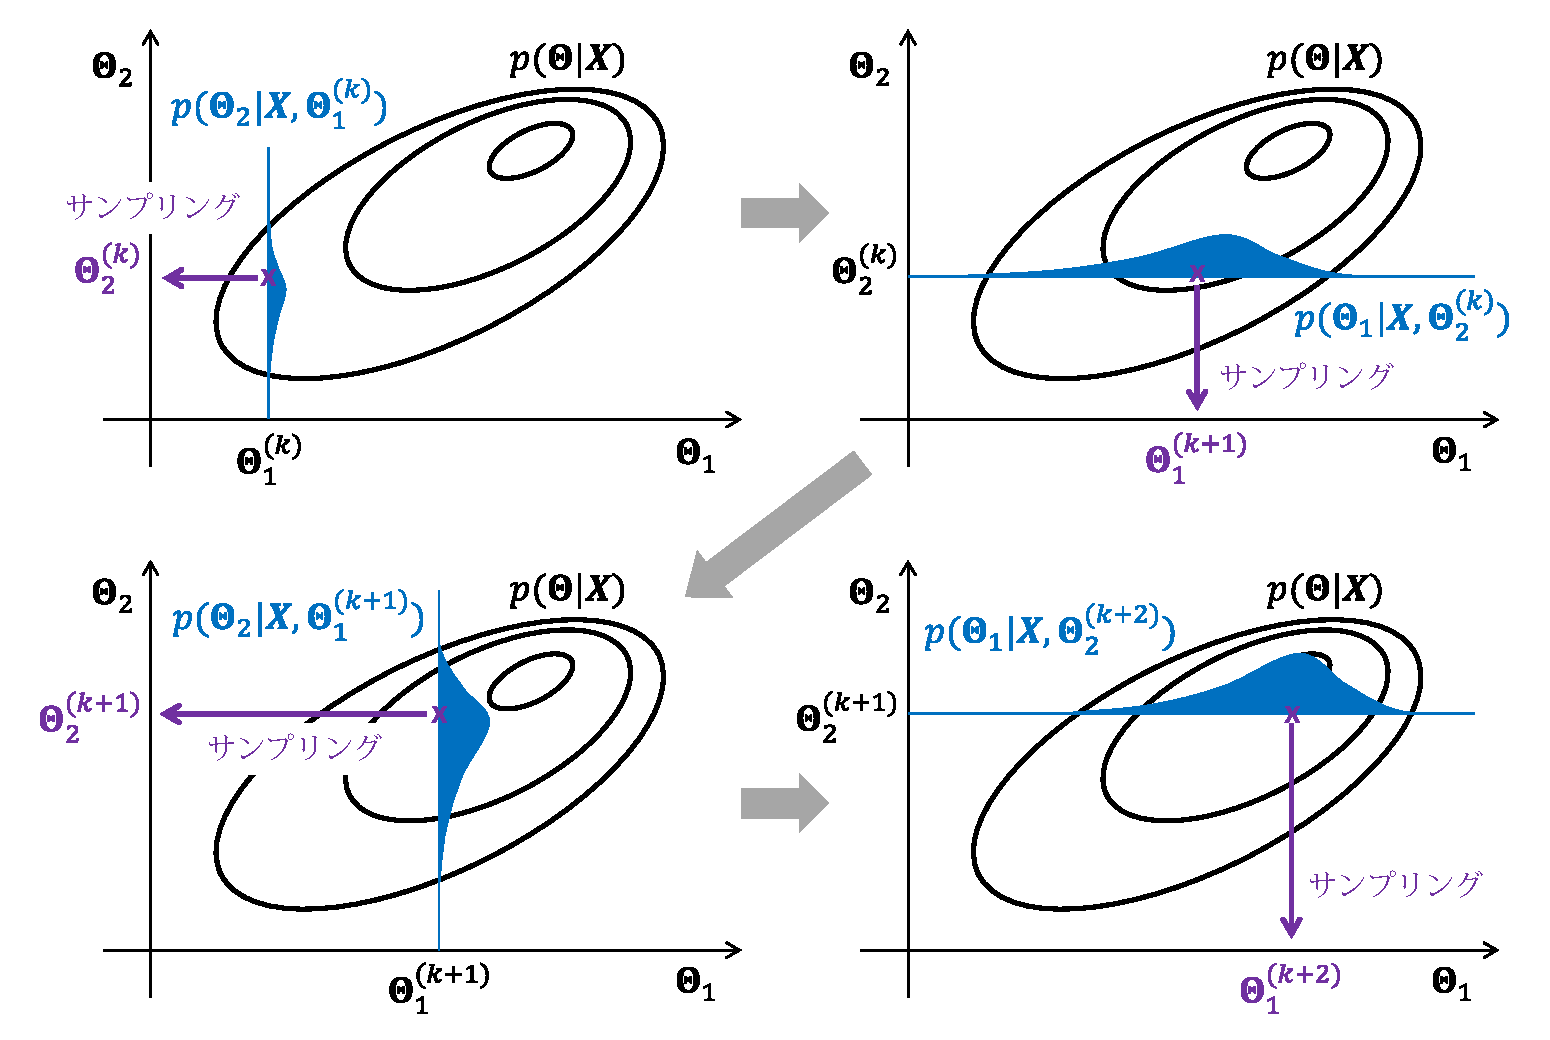
\includegraphics[width=.98\linewidth]{sections/optimization/gibbs_sampling}
\caption{ギブスサンプリングによるパラメータの更新($\bm\Theta=\{\bm\Theta_1,\bm\Theta_2\}$の場合).}
\label{fig:gibbs_sampling}
\end{figure}

より一般に,あるベイズモデル$p(\bm{X},\bm\Theta)=p(\bm{X}|\bm\Theta)p(\bm\Theta)$を
構成する確率変数$\bm\Theta$(パラメータや潜在変数の区別を問わない)が,
$M$個のグループ$\{\bm\Theta_1,\cdots,\bm\Theta_M\}$に分けられる場合について考えます.
このとき,事後分布$p(\bm\Theta|\bm{X})$に従う確率変数$\bm\Theta$のサンプルを得るには,
各$m$について
\begin{align}
\bm\Theta_m
\sim
p(\bm\Theta_m | \bm{X},\bm\Theta_{\neg m})
\end{align}
を繰り返すことになります(\reffig{fig:gibbs_sampling}).
VBとは異なり,理論上は,分割数$M$がいくらであっても,
正しく$p(\bm\Theta|\bm{X})$に従う確率変数$\bm\Theta$のサンプルが得られます.
しかし,$M$が小さいほど,$p(\bm{Z},\bm\Theta|\bm{X})$の増加が収束するのが早く,
効率的に$\bm\Theta$の最適化を行うことができます.

\subsection{ベイズ推定:周辺化ギブスサンプリング}

周辺化ギブスサンプリング (collapsed Gibbs sampling) は,
確率モデルを構成する確率変数のうちの一部を周辺化したうえで,
残りの確率変数に対してギブスサンプリングを行う手法です.
潜在変数モデルに対して適用する場合は,
全ての確率変数の事後分布$p(\bm{Z},\bm\Theta|\bm{X})$からではなく,
パラメータ$\bm\Theta$を積分消去 (marginalize out, collapse) した
潜在変数$\bm{Z}$の事後分布$p(\bm{Z}|\bm{X})$からサンプリングを行います.
事後分布の次元が小さくなっているため,
通常のギブスサンプリングより収束が早くなる利点があります.

周辺化ギブスサンプリングを用いるには,二つの条件があります.
まず,パラメータ$\bm\Theta$が容易に積分消去できることです.
すなわち,ベイズモデル$p(\bm{X},\bm{Z},\bm\Theta)
= p(\bm{X}|\bm{Z},\bm\Theta) p(\bm{Z} | \bm\Theta) p(\bm\Theta)$に対して,
積分計算
\begin{align}
p(\bm{X},\bm{Z}) = \int p(\bm{X}|\bm{Z},\bm\Theta) p(\bm{Z} | \bm\Theta) p(\bm\Theta) d\bm\Theta
\end{align}
を行う必要があります.
多くの場合,観測変数$\bm{X}$の生成モデル$p(\bm{X}|\bm{Z},\bm\Theta)$と
潜在変数$\bm{Z}$の生成モデル$p(\bm{Z} | \bm\Theta)$は独立したパラメータを持ち,
それぞれ独立した事前分布を与えることが多いでしょう.
このとき,ベイズモデルは$p(\bm{X},\bm{Z},\bm\Theta_1,\bm\Theta_2) 
= p(\bm{X}|\bm{Z},\bm\Theta_1) p(\bm{Z} | \bm\Theta_2) p(\bm\Theta_1) p(\bm\Theta_2)$となり,
\begin{align}
p(\bm{X},\bm{Z}) 
&= 
\int p(\bm{X}|\bm{Z},\bm\Theta_1) p(\bm\Theta_1) d\bm\Theta_1 
\int p(\bm{Z} | \bm\Theta_2) p(\bm\Theta_2) d\bm\Theta_2
\nonumber\\
&=
p(\bm{X}|\bm{Z}) p(\bm{Z})
\end{align}
を計算する必要があります.
$p(\bm\Theta_1)$および$p(\bm\Theta_2)$に共役事前分布を用いた場合は,
この積分は容易に解析的に計算できます.

もう一つの条件は,
事後分布$p(\bm{Z}|\bm{X})$に対して容易にギブスサンプリングが適用できることです.
具体的には,潜在変数$\bm{Z}$が$N$個のグループ$\{\bm{Z}_1,\cdots,\bm{Z}_N\}$に分けられるとすると,
各$n$について,
\begin{align}
\bm{Z}_n
\sim
p(\bm{Z}_n | \bm{X},\bm{Z}_{\neg n})
\end{align}
を繰り返しますが,
このとき,$p(\bm{Z}_n | \bm{X},\bm{Z}_{\neg n})$が解析的に計算でき,
簡単にサンプリングできる形の確率分布であることが必要です.
多くのモデルでは,$N$個の独立な観測変数$\bm{X}=\{\bm{x}_1,\cdots,\bm{x}_N\}$が与えられた時に,
対応する$N$個の潜在変数$\bm{Z}=\{\bm{z}_1,\cdots,\bm{z}_N\}$が仮定されています.
このとき,ある観測変数$\bm{x}_n$に対応する潜在変数$\bm{z}_n$に着目し,
これ以外の潜在変数$\bm{Z}_{\neg n}$の値が全て既知とした場合に,
$\bm{z}_n \sim p(\bm{z}_n | \bm{X}, \bm{Z}_{\neg n})$として,
$\bm{z}_n$の値を更新することを全ての$n$について繰り返します.

\subsection{超パラメータの最適化}

ベイズモデル$p(\bm{X}|\bm\Theta)p(\bm\Theta)$においては,
事前分布$p(\bm\Theta)$を適切に設定する必要があります.
ここで,事前分布にもパラメータ$\bm\alpha$が存在することから,
$p(\bm\Theta)$を$p(\bm\Theta|\bm\alpha)$と書くことにして,
$\bm\alpha$の決定方法について考えます.
ベイズモデルの観点からは,
$\bm\alpha$は超パラメータ (hyperparameter) と呼ばれます.
パラメータ$\bm\Theta$に関する事前知識があまりない場合は,
無情報事前分布 (noninformative prior distribution) に近い
事前分布を用いることが一般的です.
このとき,パラメータ$\bm\Theta$の事後分布は,
ほとんど事前分布の影響を受けず,
観測データ$\bm{X}$のみで決定されます.
一方,事前分布自体を最適化したい場合には,主に三つのアプローチがあります.
\begin{description}
\item[経験ベイズ (empirical Bayes)] \ \\
経験ベイズ法は,第二種の最尤推定 (type-II maximum likelihood estimation) とも呼ばれ,
観測データ$\bm{X}$に対する超パラメータ$\bm\alpha$の尤度関数$p(\bm{X}|\bm\alpha)$を
最大化するような$\bm\alpha^*$を求めます.
\begin{align}
\bm\alpha^* 
= \argmax_{\bm\alpha} p(\bm{X}|\bm\alpha)
= \argmax_{\bm\alpha} \int p(\bm{X}|\bm\Theta) p(\bm\Theta|\bm\alpha) d\bm\Theta
\label{fig:eb_argmax}
\end{align}
このとき,$p(\bm{X}|\bm\alpha)$は,
$\bm\Theta$から見れば「周辺」尤度関数となっており,
多くの現実的なモデルでは,積分計算を解析的に行うことが困難です.
このような場合でも,VBを用いて
\refeq{eq:vb_lower_bound}に示す通り
$p(\bm{X}|\bm\alpha)$の下限関数$\mathcal{L}(q(\bm{Z}),q(\bm\Theta),\bm\alpha)$を導出すれば,
補助関数法(\refsec{sec:auxiliary_function})の原理に従って,
$q(\bm{Z})$,$q(\bm\Theta)$および$\bm\alpha$を交互に最適化することが可能になります.
ただし,最適化すべき関数$\mathcal{L}(q(\bm{Z}),q(\bm\Theta),\bm\alpha)$は
解析的に導出できたとしても,
一般に,$\mathcal{L}(q(\bm{Z}),q(\bm\Theta),\bm\alpha)$は$\bm\alpha$に関する複雑な関数となっており,
最適な$\bm\alpha^*$を解析的に求めることは困難です.
したがって,最急降下法(\refsec{sec:steepest_descent}),
ニュートン法(\refsec{sec:newton}),
準ニュートン法(\refsec{sec:quasi_newton})などの
一般的な反復最適化技法を用いる必要があります.
乗法更新アルゴリズム(\refsec{sec:multiplicative_update})が利用できる場合もあります.
\item[階層ベイズ (hierarchical Bayes)] \ \\
階層ベイズ法では,超パラメータ$\bm\alpha$に対する事前分布
(超事前分布と呼ぶ)$p(\bm\alpha)$を導入して,
事後分布$p(\bm\alpha|\bm{X})$を計算します.
\begin{align}
 p(\bm\alpha|\bm{X}) 
 &= \frac{p(\bm{X}|\bm\Theta)p(\bm\Theta|\bm\alpha)p(\bm\alpha)}{p(\bm{X})}
 \nonumber\\
 &= \frac{p(\bm{X}|\bm\Theta)p(\bm\Theta|\bm\alpha)p(\bm\alpha)}
 {\int\int p(\bm{X}|\bm\Theta)p(\bm\Theta|\bm\alpha)p(\bm\alpha) d\bm\Theta d\bm\alpha}
\label{eq:hb_posterior}
\end{align}
経験ベイズ法では,超パラメータ$\bm\alpha$を点推定しているのに対し,
階層ベイズ法では,未知である$\bm\alpha$の不確実性を適切に取り扱う点で優れています.
しかし,一般に,\refeq{eq:hb_posterior}の分母の積分計算は極めて困難であり,
VBもギブスサンプリングも利用できない場合がほとんどです.
そのため,一般には,MCMCを用いたサンプリングが行われます.

この方法では,超パラメータ$\bm\alpha$のベイズ推定が可能になる代わりに,
超事前分布$p(\bm\alpha)$自体を適切に設定するという新たな問題が生まれます.
しかし,現実には,超パラメータ$\bm\alpha$に関する事前知識はほとんどないことが多く,
$\bm\alpha$に対しては無情報事前分布がよく用いられます.
このように,ベイズモデルにおいては,階層が上がるにつれて,
パラメータの抽象度が高くなるので,
曖昧性の高い超事前分布を設定しても問題ないことがほとんどです.
むしろ,事前知識がないにもかかわらず,超事前分布を少し変えるだけで,
$\bm\Theta$や$\bm\alpha$の推定に大きな影響が出る場合,
そのベイズモデルは適切ではない可能性があります.
\item[ベイズ最適化 (Bayesian optimization)] \ \\
経験ベイズ法が,周辺尤度$p(\bm{X}|\bm\alpha)$を最大化する
超パラメータ$\bm\alpha$を求めていたのに対して,
ベイズ最適化では,任意の目的関数を最大化する
$\bm\alpha^*$を効率的に探索する方法を提供します.
例えば,ベイズモデルに基づく音声認識システムであれば,
周辺尤度ではなく,より直接的に,
音声認識率を最大化するような$\bm\alpha^*$を求めたいでしょう.
もし,$\bm\alpha$が高々2, 3個の変数から構成されている場合は,
グリッドサーチが利用できるかもしれません.
しかし,変数の個数が増えてくると,試すべき組み合わせの数は指数的に爆発します.
そもそも,$f(\bm\alpha)$を1回評価するのに時間がかかる場合は,
試行回数をできる限り削減することが望まれます.

ベイズ最適化では,音声認識システムを,
$\bm\alpha$を引数に取り,認識率を返す未知のブラックボックス関数$f(\bm\alpha)$とみなします.
これまでの$N$回の試行結果から,$N$個の入力$\{\bm\alpha^{(1)},\cdots,\bm\alpha^{(N)}\}$に対する
関数値$\{f(\bm\alpha^{(1)}),\cdots,f(\bm\alpha^{(N)})\}$が分かっていたとします.
このとき,次に試すべき$\bm\alpha^{(N+1)}$として,
$f(\bm\alpha)$が大きな値をとることが判明している$\bm\alpha$の周辺を調査することが考えられます.
一方,まだ探索が進んでいない空間に,
より大きな$f(\bm\alpha)$をとりうる$\bm\alpha$が存在する可能性もあります.
ベイズ最適化では,$f(\bm\alpha)$がガウス過程 (Gaussian process) に従うと仮定したうえで,
活用 (exploitation) と探索 (exploration) のトレードオフを考慮しながら,
次に試すべき$\bm\alpha^{(N+1)}$を提案します.
この提案方法にはいくつかの方法が知られており\cite{a,b,c,d},
どれが良いかは関数の性質によって異なります.
汎用的な最適化技法であるため,
ソフトウェアも公開されており,簡単に利用可能です\cite{soft}.
\end{description}

\section{混合ベイズモデルの学習}

本節では,代表的な潜在変数モデルである
混合ガウスモデル (Gaussian mixture model, GMM) を例に,
EMアルゴリズム,VB,ギブスサンプリング,周辺化ギブスサンプリングを
適用する方法について解説します.
GMMは最も基本的かつ重要な確率モデルの一つであり,
音響信号処理分野における様々な場面で利用されています.
\begin{description}
\item[多次元特徴量ベクトルの分布の学習] \ \\
音響信号から抽出した多次元の特徴量ベクトルの分布を表現するうえで,
GMMは最初に検討すべき標準的なモデルです.
例えば,音声認識システムにおいては,
各音素について,音声スペクトルから抽出した13次元程度の
メル周波数ケプストラム係数 (mel-frequency cepstrum coefficients)
の分布をGMMを用いて表現するのが一般的でした
(近年は深層学習を用いる場合が主流)\cite{speech_recognition}.
また,楽曲検索システムにおいて,
ある楽曲と類似した楽曲を検索するうえで,
各楽曲の音楽音響信号から抽出した音響的特徴量の分布をGMMで表現し,
二つのGMM間の距離を計算することがしばしば行われます\cite{music_retrieval}.
\item[基本周波数推定]
\item[マルチチャネル音源分離]
\end{description}

\begin{figure}[t]
\centering
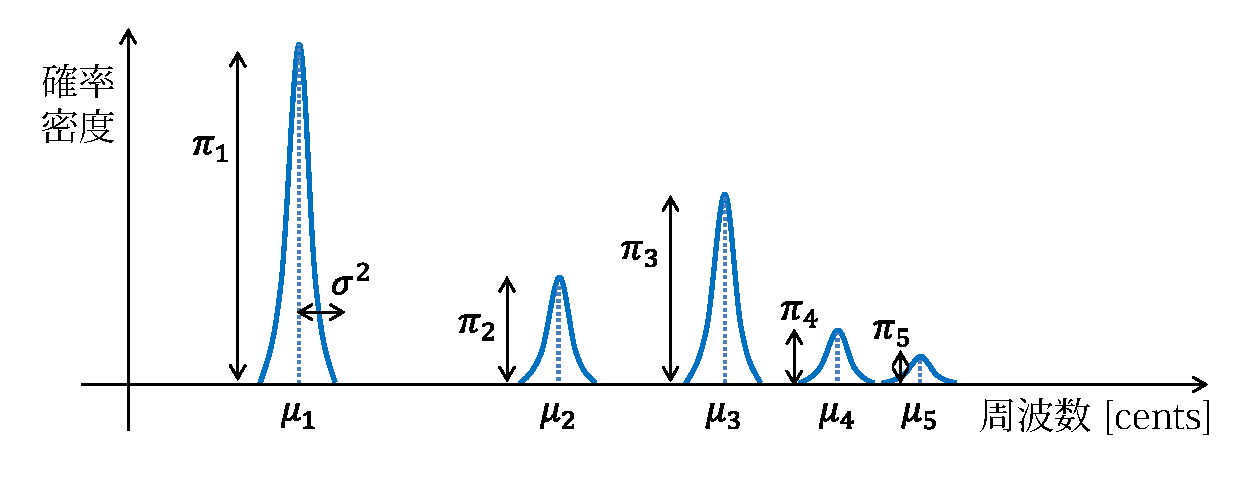
\includegraphics[width=.9\linewidth]{sections/optimization/gmm_f0_estimation}
\vspace{-2mm}
\caption{調波構造を表現するGMM.
観測データ$\bm{X}$として振幅スペクトルが与えられた時に,
各種パラメータ$\bm\Theta=\{\mu_1,\cdots,\mu_5,\pi_1,\cdots,\pi_5,\sigma^2\}$を
最尤推定あるいはベイズ推定する問題を解けば,基本周波数$\mu_1$が推定できる.}
\label{fig:gmm_f0_estimation}
\end{figure}

\begin{figure}[t]
\centering
\includegraphics[width=.9\linewidth]{sections/optimization/gmm_separation}
\vspace{-2mm}
\caption{時間周波数クラスタリングに基づくマルチチャネル音源分離.}
\label{fig:gmm_separation}
\end{figure}


比較的単純にもかかわらず,柔軟な表現力を持つことから,

観測データとして$N$個の$D$次元ベクトル
$\bm{X} = \{\bm x_{1},\cdots,\bm x_{N}\}$を考える.
また,観測データ$\bm X$に対応する潜在変数系列
を$\bm{Z} = \{\bm z_{1},\cdots,\bm z_{N}\}$とする.
ここでは可算無限個のガウス分布の混合を許容するモデルを考えているので,
$\bm z_{n}$は選ばれたガウス分布に対応する次元のみが1で他は0である
ような$K \rightarrow \infty$次元のベクトルである.
このとき,グラフィカルモデルから変数間の条件つき独立性を考慮すると,
完全な同時分布は
\begin{eqnarray}
p(\bm{X},\bm{Z},\bm\pi,\bm\mu,\bm\Lambda) 
 = 
 p(\bm{X}|\bm{Z},\bm\mu,\bm\Lambda)  
 p(\bm{Z}|\bm\pi) 
 p(\bm\pi)
 p(\bm\mu,\bm\Lambda) 
 \label{eq:jointp}
\end{eqnarray}
で与えられる.
ここで,$\bm\pi$は無限個のガウス分布に対する混合係数で,
無限次元のベクトルである.
$\bm\mu$および$\bm\Lambda$は各ガウス分布のパラメータ
(平均$\bm\mu_{k}$および分散$\bm\Lambda_{k}^{-1}$)である.
まず,第一項には尤度を設定する.
\begin{eqnarray}
 p(\bm{X}|\bm{Z},\bm\mu,\bm\Lambda) 
  &=& \prod_{n=1}^{N} \prod_{k=1}^{\infty} 
      \mathcal{N}\left(\bm{x}_{n}\big|\bm\mu_{k},\bm\Lambda_{k}^{-1}\right)^{z_{n,k}}
      \label{eq:pxzmula}
\end{eqnarray}
いま,集中度$\alpha$・基底測度$G_0$である
ディリクレ過程$\mbox{DP}(\alpha,G_0)$を考える.
基底測度$G_0$として,
$\bm{\mu},\bm{\Lambda}$上の{\bf 連続分布}を与えることにする.
このとき,$\bm{\mu},\bm{\Lambda}$上の別の分布$G$を$G \sim \mbox{DP}(\alpha,G_0)$として
生成することができる.
こうすると,$G$は{\bf 可算無限次元の離散分布}となり,
ある次元$k$の重みが$\pi_k$に,
実現値が$\bm\mu_k,\bm\Lambda_k$に対応する.
すなわち,無限混合ガウス分布が具体的にひとつ定まる.
ここで,$G_0$は$G$の期待値となっており,
$\alpha$が大きいほど$G_0$に近くなる.
%すなわち,$\alpha$は逆分散のように振る舞う.
ディリクレ過程の一つの実現方法として,
ここではStick-Breaking Construction (SB過程) を用いる.
SBCは変分ベイズ法を適用するうえで都合が良いDPの表現方法である.
このとき,混合係数$\pi_k$は次式で与えられる.
\begin{eqnarray}
 \pi_k &=& v_k \prod_{k'=1}^{k-1} (1 - v_{k'}) \\
 v_{k} &\sim& \mbox{Beta}(1, \alpha)
\end{eqnarray}
このように$\pi_k$を$v_k$に変数変換を行うことで,
\refeq{eq:jointp}の第二項および第三項の積$p(\bm{Z},\bm\pi)=p(\bm{Z}|\bm\pi)p(\bm\pi)$は
積$p(\bm{Z},\bm{v})=p(\bm{Z}|\bm{v})p(\bm{v})$として書き直せる.
このとき,各項は以下で与えられる.
\begin{eqnarray}
 p(\bm{Z}|\bm{v}) 
  &=& \prod_{n=1}^{N} \prod_{k=1}^{\infty}  
      \pi_{k}^{z_{n,k}} 
      \nonumber \\ 
  &=& \prod_{n=1}^{N} \prod_{k=1}^{\infty}
      \left(v_k \prod_{k'=1}^{k-1} (1 - v_{k'})\right)^{z_{n,k}}
      \nonumber \\ 
  &=& \prod_{n=1}^{N} 
      \left(\prod_{k=1}^{\infty} v_k^{z_{n,k}}\right)
      \left(\prod_{k=1}^{\infty} \prod_{k'=1}^{k-1} (1 - v_{k'})^{z_{n,k}}\right)
      \nonumber \\ 
  &=& \prod_{n=1}^{N} 
      \left(\prod_{k=1}^{\infty} v_k^{z_{n,k}}\right)
      (1 - v_1)^{z_{n,2}} 
      \bigl((1 - v_1)(1 - v_2)\bigr)^{z_{n,3}}
      \bigl((1 - v_1)(1 - v_2)(1 - v_3)\bigr)^{z_{n,4}}
      \cdots
      \nonumber \\
  &=& \prod_{n=1}^{N} 
      \prod_{k=1}^{\infty}
      v_k^{z_{n,k}} 
      (1 - v_k)^{\sum_{k' = k+1}^{\infty} z_{n,k'}}
      \label{eq:pzv}
      \\
 p(\bm{v}) 
  &=& \prod_{k=1}^{\infty} \mbox{Beta}(v_k|1, \alpha)
   =  \prod_{k=1}^{\infty} \frac{\Gamma(1 + \alpha)}
      {\Gamma(1)\Gamma(\alpha)} v_k^{1-1} (1 - v_k)^{\alpha - 1}
   =  \prod_{k=1}^{\infty} \alpha (1 - v_k)^{\alpha - 1}
  \label{eq:pv}
\end{eqnarray}
\refeq{eq:jointp}の第四項には,基底測度$G_0$として,
ガウス分布の共役事前分布であるガウス・ウィシャート分布を設定する.
\begin{eqnarray}
 p(\bm\mu,\bm\Lambda)
  &=&
  \prod_{k=1}^{\infty}
  \mathcal{N}\left(\bm\mu_{k}\big|\bm{m}_0,(b_0\bm\Lambda_{k})^{-1}\right)
  \mathcal{W}\left(\bm\Lambda_{k}\big|\bm{W}_0,c_0\right)
  \label{eq:pmu}
\end{eqnarray}
ここで,$\bm{m}_0$,$b_0$,$\bm{W}_0$および$c_0$は
ハイパーパラメータである.
通常はすべての$k$について同じ事前分布を与える.

\subsection{最尤推定:EMアルゴリズム}

\subsection{ベイズ推定:変分ベイズ法}

\section{変分事後分布}

ベイズ推定の目的は,観測データ$\bm{X}$が与えられたときに,
事後分布$p(\bm{Z},\bm{v},\bm\mu,\bm\Lambda|\bm{X})$を
求めることである.
しかし,これを解析的に計算することは困難なので,
変分事後分布$q(\bm{Z},\bm{v},\bm\mu,\bm\Lambda)$
を導入し,できるかぎり真の事後分布に近づけるよう最適化を行いたい.
いま,変分事後分布の潜在変数とパラメータへの因子分解
\begin{eqnarray}
 q(\bm{Z},\bm{v},\bm\mu,\bm\Lambda) 
  = q(\bm{Z}) q(\bm{v},\bm\mu,\bm\Lambda) 
 \label{eq:approx}
\end{eqnarray}
を考える.これがベイズ推定に変分ベイズ法を適用する場合の唯一の仮定である.
変分ベイズ法は,事後分布の関数形を解析的に導出可能な形に制限し,
その中で最適なものを探す手法である.
これはさらに
\begin{eqnarray}
q(\bm{Z},\bm{v},\bm\mu,\bm\Lambda) 
= q(\bm{Z}) q(\bm{v}) q(\bm\mu|\bm\Lambda) q(\bm\Lambda)
\end{eqnarray}
と因子分解できる.
あとで見るように,これは仮定や近似ではなく,
グラフィカルモデルの構造から必然的に導かれる.

%また,$p(\bm{v})$は$p(\bm{Z}|\bm{v})$の共役事前分布になっているので,
%因子$q(\bm{v})$は可算無限個のベータ分布の積になるはずである.
%すなわち,$\bm\alpha_{k}=\{\alpha_{k,1},\alpha_{k,2}\}$を
%$v_k$に対応する変分事後分布(ベータ分布)のパラメータとすると,
%\begin{eqnarray}
% q(\bm{v}) = \prod_{k=1}^{K} q(v_k|\bm\alpha_k) 
%  = \prod_{k=1}^{K} \mbox{Beta}(v_k|\bm\alpha_k)
%\end{eqnarray}
%と表わせる.

無限混合モデルに変分ベイズ法を適用する場合,
さらに,十分に大きいある整数$k>K$について,
\begin{eqnarray}
 q(z_{n,k>K}) = 0
\end{eqnarray}
を仮定し,可算無限個あるガウス分布のうち,
観測データ中には$K+1$番目以降に割り当てられるサンプルが存在しなかったとする.
ここで,混合数の打ち切り (truncate) は,
事前分布$p(\bm{v})$,真の事後分布$p(\bm{v}|\bm{X})$
あるいは変分事後分布$q(\bm{v})$に対してではなく,
変分事後分布$q(\bm{Z})$に対して行っていることに注意する.
この仮定のもとでは,$k \le K$における$q(v_k)$を考慮すれば十分であり,
$K$の値に関して推論結果がネストされることになる
(大きな$K$における結果が小さな$K$における結果を含む).
したがって,実質的には有限混合モデルに対する事後分布推論を行うが,
理論的には完全な無限混合モデルとして取り扱うことができる.
一方,$q(v_K=1) = 1$とし,$K+1$回以上のStick Breakingが発生しないとする仮定では,
推論結果はネストされないという違いがある.

このように,SBCに基づくベイズ推論では,
\refeq{eq:pmu}のように,基底測度$G_0$から得られる離散分布$G$として,
十分に多い$K$個のガウス分布を考慮する必要がある.
一方,別のディリクレ過程の実現方法であるChinese Restaurant Process (CRP) では,
過去の潜在変数系列$\{\bm{z}_1,\cdots,\bm{z}_n\}$から次の潜在変数$\bm{z}_{n+1}$の予測分布を考える.
CRPは,有限混合モデルにおけるパラメータ$\bm\pi$を積分消去し,
混合数を無限としたときの極限と解釈できる.
MCMCを利用すれば,混合数が増加した場合に,
随時新たな要素分布$G$をサンプルして増やしていくことができる.

\subsection{VB-Eステップ}\label{sec:vb-e}

まず,VB-Eステップでは因子$q(\bm{Z})$について考える.
一般的な結果を用いると,最適な因子は
\begin{eqnarray}
 \log q^*(\bm{Z}) 
  = \mathbb{E}_{\bm{v},\bm\mu,\bm\Lambda}
  \left[\log p(\bm{X},\bm{Z},\bm{v},\bm\mu,\bm\Lambda)\right] + \mbox{const.}
\end{eqnarray}
で与えられる.式(\ref{eq:jointp})を代入し,
右辺で変数$\bm{Z}$への依存関係だけに興味があることに注意すると,
\begin{eqnarray}
 \log q^*(\bm{Z}) = 
    \mathbb{E}_{\bm\mu,\bm\Lambda} \left[\log p(\bm{X}|\bm{Z},\bm\mu,\bm\Lambda) \right]
  + \mathbb{E}_{\bm{v}} \left[\log p(\bm{Z}|\bm{v})\right]
  + \mbox{const.}
\end{eqnarray}
を得る.$\bm{Z}$に依存関係のない項は
すべて正規化定数$\mbox{const.}$に含まれるので,
必要に応じて計算すればよい.
\begin{eqnarray}
 \log q^*(\bm{Z}) 
  &=& \mathbb{E}_{\bm\mu,\bm\Lambda}
   \left[
    \sum_{n=1}^{N} \sum_{k=1}^{K}
    z_{n,k} 
    \log \mathcal{N}\left(\bm{x}_{n}\big|\bm\mu_{k},\bm\Lambda_{k}^{-1}\right)
   \right]
   \nonumber\\
  && + \ \mathbb{E}_{\bm{v}} 
   \left[
    \sum_{n=1}^{N} \sum_{k=1}^{K}
     \left(
     z_{n,k} \log v_k
     + z_{n,k} \sum_{k' = 1}^{k - 1} \log (1 - v_{k'})
     \right)
   \right] 
   + \mbox{const.} 
   \nonumber\\
  &=& \sum_{n=1}^{N} \sum_{k=1}^{K}
   z_{n,k}
   \left(
    \mathbb{E}_{v_k}[\log v_k] 
    + \sum_{k' = 1}^{k - 1} \mathbb{E}_{v_{k'}}[\log (1 - v_{k'})] 
    + \ \mathbb{E}_{\bm\mu_k,\bm\Lambda_k}
    \left[\log \mathcal{N}\left(\bm{x}_{n}\big|\bm\mu_{k},\bm\Lambda_{k}^{-1}\right)\right]
   \right) 
   + \mbox{const.} 
   \nonumber\\
  &=& \sum_{n=1}^{N} \sum_{k=1}^{K}
   z_{n,k} \log \rho_{n,k} 
   + \mbox{const.} 
   \label{eq:lqz}
\end{eqnarray}
ここで,
\begin{eqnarray}
 \log \rho_{n,k} 
 =    \mathbb{E}_{v_k}[\log v_k] 
    + \sum_{k' = 1}^{k - 1} \mathbb{E}_{v_{k'}}[\log (1 - v_{k'})] 
    + \ \mathbb{E}_{\bm\mu_k,\bm\Lambda_k}
    \left[\log \mathcal{N}\left(\bm{x}_n\big|\bm\mu_{k},\bm\Lambda_{k}^{-1}\right)\right]
 \label{eq:rho}
\end{eqnarray}
とした.
上式中の期待値はVB-Mステップにおいて
\refeq{eq:epi1},\refeq{eq:epi2}および\refeq{eq:egauss}として得られる.
\newpage

\refeq{eq:lqz}の両辺の対数をとると
\begin{eqnarray}
 q^*(\bm{Z}) 
 \propto
 \prod_{n=1}^{N}\prod_{k=1}^{K} \rho_{n,k}^{z_{n,k}}
\end{eqnarray}
を得る.この分布は正しく正規化されている必要があること,
任意の$n,k$の値について$z_{n,k}$は1あるいは0をとり,
すべての$k$にわたる和が$1$であることに注意すると
\begin{eqnarray}
 q^*(\bm{Z}) 
 =
 \prod_{n=1}^{N}\prod_{k=1}^{K}
 \gamma_{n,k}^{z_{n,k}} 
 \label{eq:qz}
\end{eqnarray}
を得る.ここで,量$\bm\gamma_{n}$はデータ$n$に対する要素分布$k$の負担率であり
\begin{eqnarray}
 \gamma_{n,k} = \frac{\rho_{n,k}}{\sum_{k'=1}^{K}\rho_{n,k'}}
\end{eqnarray}
で与えられる.
式(\ref{eq:qz})で与えられる因子$q(\bm{Z})$の最適解$q^*(\bm{Z})$は,
式(\ref{eq:pzv})で与えられる事前分布$p(\bm{Z}|\bm{v})$と
同じ形をしている.
$q(\bm{Z})$の関数形に関する仮定を導入していないにもかかわらず,
式(\ref{eq:approx})の因子分解とグラフィカルモデルの構造からこの結果は必然的に導かれる.
\refeq{eq:qz}から,潜在変数$\bm{z}_{n}$は
パラメータ$\bm\gamma_{n}$をもつ多項分布に従うことが分かる.
したがって,$z_{n,k}$の期待値は次式で与えられる.
\begin{eqnarray}
 \mathbb{E}_{\bm{z}_{n}}[z_{n,k}] = \gamma_{n,k} 
  \label{eq:ez}
\end{eqnarray}

\subsection{VB-Mステップ}\label{sec:vb-m}

次に,VB-Mステップでは因子$q(\bm{v},\bm\mu,\bm\Lambda)$について考える.
一般的な結果を再度用いると,最適な因子は
\begin{eqnarray}
 \log q^*(\bm{v},\bm\mu,\bm\Lambda)
 &=& \mathbb{E}_{\bm{z}}
  \left[\log p(\bm{v}) + \log p(\bm{Z}|\bm{v})\right]
  + \mathbb{E}_{\bm{z}}
  \left[\log p(\bm\mu,\bm\Lambda) + \log p(\bm{X}|\bm{Z},\bm\mu,\bm\Lambda)\right]
  + \mbox{const.} 
 \nonumber\\
 &=& \log p(\bm{v})
  + \mathbb{E}_{\bm{z}}\left[\log p(\bm{Z}|\bm{v})\right] 
  + \log p(\bm\mu,\bm\Lambda)
  + \mathbb{E}_{\bm{z}}
  \left[\log p(\bm{X}|\bm{Z},\bm\mu,\bm\Lambda)\right]
  + \mbox{const.}
  \label{eq:qpiphitaumulambda}
\end{eqnarray}
で与えられる.ここで,VB-Eステップの\refeq{eq:ez}を用いると,
\refeq{eq:qpiphitaumulambda}中の期待値は次式で計算できる.
\begin{eqnarray}
 \mathbb{E}_{\bm{z}}\left[\log p(\bm{Z}|\bm{v})\right] 
  &=& \mathbb{E}_{\bm{z}}
   \left[\sum_{n=1}^{N}\sum_{k=1}^{K}
   \left(
   z_{n,k} \log v_k + \left(\sum_{k'=k+1}^{K} z_{n,k'} \right) \log (1 - v_k)
   \right)
   \right]
   \nonumber\\
  &=& \sum_{n=1}^{N}\sum_{k=1}^{K}
   \left(
   \gamma_{n,k} \log v_k
   + \left(\sum_{k'=k+1}^{K} \gamma_{n,k'} \right) \log (1 - v_k)
   \right)
   \\
 \mathbb{E}_{\bm{z}}\left[\log p(\bm{X}|\bm{Z},\bm\mu,\bm\Lambda)\right] 
  &=& \mathbb{E}_{\bm{z}}
   \left[\sum_{n=1}^{N}\sum_{k=1}^{K}
   z_{n,k}
   \log \mathcal{N}\left(\bm{x}_{n}\big|\bm\mu_{k},\bm\Lambda_{k}^{-1}\right)
   \right]
   \nonumber\\
  &=& \sum_{n=1}^{N}\sum_{k=1}^{K}
   \gamma_{n,k}
   \log \mathcal{N}
   \left(\bm{x}_{n}\big|\bm\mu_{k},\bm\Lambda_{k}^{-1}\right)
\end{eqnarray}
\refeq{eq:qpiphitaumulambda}をよく観察すると,$\bm{v}$のみを含む項,
$\bm\mu,\bm\Lambda$のみを含む項の和に分解できることがわかる.
それぞれはさらに$k$を含む項ごとの和に分解できる.
すなわち,最適な因子$q^*(\bm{v},\bm\mu,\bm\Lambda)$は
\begin{eqnarray}
 q^*(\bm{v},\bm\mu,\bm\Lambda)
  = 
  \prod_{k=1}^{K} q^*(v_k) 
  \prod_{k=1}^{K} q^*(\bm\mu_{k},\bm\Lambda_{k})
  \label{eq:qqq}
\end{eqnarray}
と分解できる.
このような分解が可能であることもグラフィカルモデルの構造から必然的に導かれる.

\refeq{eq:qpiphitaumulambda}に\refeq{eq:pv}および\refeq{eq:pmu}を代入し,
\refeq{eq:qqq}と比較することで,最適な因子$q^*(\bm{v})$は
\begin{eqnarray}
 \log q^*(v_k) 
  &=& 
  \left(1 + \sum_{n=1}^{N} \gamma_{n,k} - 1 \right) \log v_k
   + \left(\alpha + \sum_{n=1}^{N}\sum_{k'=k+1}^{K} \gamma_{n,k'} - 1 \right) \log (1 - v_k)   
   + \mbox{const.}
   \label{eq:qv}
\end{eqnarray}
で与えられる.
両辺の指数をとると,最適な因子はベータ分布
\begin{eqnarray}
 q^*(v_k) = \mbox{Beta}(v_k|\bm\alpha_k)
\end{eqnarray}
で与えられることが分かる.これらはやはり
\refeq{eq:pv}で与えられる事前分布と同じ形をしている.
このとき,ベータ分布のパラメータ$\bm\alpha_k$は
\begin{eqnarray}
 \alpha_{k,1} 
 &=& 1 + \sum_{n=1}^{N} \gamma_{n,k}
 \label{eq:alpha1}\\
 \alpha_{k,2}
 &=& \alpha + \sum_{n=1}^{N}\sum_{k'=k+1}^{K} \gamma_{n,k'}
 \label{eq:alpha2}
\end{eqnarray}
で定まる.
ここで,変数$v_k$がパラメータ$\bm\alpha_k$をもつ
ベータ分布に従うことに着目すると,
$\log v_k$および$\log (1 - v_k)$の期待値は標準的な公式から
\begin{eqnarray}
 \mathbb{E}_{v_k}[\log v_k] 
  &=& \psi\left(\alpha_{k,1}\right) - \psi\left(\alpha_{k,1} + \alpha_{k,2}\right)
  \label{eq:epi1}
 \\
 \mathbb{E}_{v_k}[\log (1 - v_k)] 
  &=& \psi\left(\alpha_{k,2}\right) - \psi\left(\alpha_{k,1} + \alpha_{k,2}\right)
  \label{eq:epi2}
\end{eqnarray}
と計算できる.ここで,$\psi(\cdot)$はディガンマ関数(対数ガンマ関数の導関数)である.

最後に,因子$q^*(\bm\mu_{k},\bm\Lambda_{k})$について考える.
事前分布として共役事前分布を与えたため,
事後分布は事前分布と同じガウス・ウィシャート分布になるはずである.
この導出を行う前に,十分統計量
\begin{eqnarray}
\mathbb{S}_{k}[1] 
&\equiv& \sum_{n=1}^{N} \gamma_{n,k}
\label{eq:s}\\
\mathbb{S}_{k}[\bm{x}] 
&\equiv& 
\sum_{n=1}^{N} \gamma_{n,k} 
\bm{x}_{n}
\label{eq:sy}\\
\mathbb{S}_{k}[\bm{x}\bm{x}^T] 
&\equiv& 
\sum_{n=1}^{N} \gamma_{n,k} 
\bm{x}_{n}\bm{x}_{n}^T
\label{eq:syy}
\end{eqnarray}
を定義しておく.
いま,\refeq{eq:qpiphitaumulambda}の右辺で
興味がある$\bm\mu_{k}$および$\bm\Lambda_{k}$を含む項を取り出すと
\begin{eqnarray}
\log q^*(\bm\mu_{k},\bm\Lambda_{k})
&=& 
\log \mathcal{N}\left(\bm\mu_{k}\big|\bm{m}_0,\left(b_0\bm\Lambda_{k}\right)^{-1}\right)
+
\log \mathcal{W}\left(\bm\Lambda_{k}\big|\bm{W}_0,c_0\right)
+
\sum_{n=1}^{N}
\gamma_{n,k}
\log \mathcal{N}\left(\bm{x}_n\big|\bm\mu_{k},\bm\Lambda_{k}^{-1}\right)
+ \mbox{const.}
\nonumber\\
&=&
\frac{1}{2}\log|\bm\Lambda_{k}|
- \frac{b_0}{2} (\bm\mu_{k} - \bm{m}_0)^T\bm\Lambda_{k}(\bm\mu_{k} - \bm{m}_0)
+
\frac{c_0 - D - 1}{2} \log|\bm\Lambda_{k}|
-\frac{1}{2}\mbox{Tr}\left(\bm{W}_0^{-1}\bm\Lambda_{k}\right)
\nonumber\\
&&
+\frac{1}{2}
\sum_{n=1}^{N} 
\gamma_{n,k} \log|\bm\Lambda_{k}|
-\frac{1}{2}
\sum_{n=1}^{N} 
\gamma_{n,k}  
(\bm{x}_n - \bm\mu_{k})^T\bm
\Lambda_{k}(\bm{x}_n - \bm\mu_{k})
+ \mbox{const.}
\label{eq:qphik}
\end{eqnarray}
を得る.まず,$p(\bm\mu_{k}|\bm\Lambda_{k})$に対応する部分,
すなわち$\bm\mu_{k}$を含む項をとりだすと
\begin{eqnarray}
\log q^*(\bm\mu_{k}|\bm\Lambda_{k})
&=& 
- \frac{b_0}{2} (\bm\mu_{k} - \bm{m}_0)^T\bm\Lambda_{k}(\bm\mu_{k} - \bm{m}_0)
-\frac{1}{2}
\sum_{n=1}^{N} 
\gamma_{n,k}  
(\bm{x}_n - \bm\mu_{k})^T\bm
\Lambda_{k}(\bm{x}_n - \bm\mu_{k})
+ \mbox{const.}
\nonumber\\
&=&
- \frac{1}{2}
\bm\mu_{k}^T \bm\Lambda_{k} \bm\mu_{k}
\left(b_0 
 + \sum_{n=1}^{N} \gamma_{n,k} 
\right)
+ \frac{1}{2} 
\bm\mu_{k}^T \bm\Lambda_{k} 
\left(
 b_0\bm{m}_0 + 
 \sum_{n=1}^{N} 
 \gamma_{n,k} \bm{x}_n
\right)
+ \frac{1}{2} 
\left(
 b_0\bm{m}_0 + 
 \sum_{n=1}^{N} 
 \gamma_{n,k} \bm{x}_n
\right)^T
\!\!\!\bm\Lambda_{k} \bm\mu_{k}
\nonumber\\
&&
- \frac{b_0}{2} \bm{m}_0^T \bm\Lambda_{k} \bm{m}_0
- \frac{1}{2} 
 \sum_{n=1}^{N} \gamma_{n,k} 
 \bm{x}_n^T \bm\Lambda_{k} \bm{x}_n
+ \mbox{const.}
\nonumber\\
&=&
-\frac{1}{2} \Bigl(b_0 + \mathbb{S}_{k}[1]\Bigr)
\left(\bm\mu_{k}^T \bm\Lambda_{k} \bm\mu_{k}
 - \bm\mu_{k}^T \bm\Lambda_{k} 
\frac{b_0\bm{m}_0 + \mathbb{S}_{k}[\bm{x}]} 
     {b_0 + \mathbb{S}_{k}[1]}
 - 
\left(
\frac{b_0\bm{m}_0 + \mathbb{S}_{k}[\bm{x}]} 
     {b_0 + \mathbb{S}_{k}[1]}\right)^T
     \!\!\!\bm\Lambda_{k} \bm\mu_{k} 
\right)
\nonumber\\
&&
- \frac{b_0}{2} \bm{m}_0^T \bm\Lambda_{k} \bm{m}_0
- \frac{1}{2} 
 \sum_{n=1}^{N} \gamma_{n,k} 
 \bm{x}_n^T \bm\Lambda_{k} \bm{x}_n
+ \mbox{const.}
\end{eqnarray}
を得る.よって,$q^*(\bm\mu_{k}|\bm\Lambda_{k})$はガウス分布
\begin{eqnarray}
q^*(\bm\mu_{k}|\bm\Lambda_{k}) = 
\mathcal{N}\left(\bm\mu_{k}\big|\bm{m}_{k},\left(b_{k}\bm\Lambda_{k}\right)^{-1}\right)
\label{eq:qmklk}
\end{eqnarray}
となることが分かり,そのパラメータは次式で定まる.
\begin{eqnarray}
b_{k} 
&=& b_0 + \mathbb{S}_{k}[1]
\label{eq:bk}\\
\bm{m}_{k}
&=& \frac{b_0\bm{m}_0 + \mathbb{S}_{k}[\bm{x}]} 
       {b_0 + \mathbb{S}_{k}[1]}
= \frac{b_0\bm{m}_0 + \mathbb{S}_{k}[\bm{x}]} 
       {b_{k}}
\label{eq:mk}
\end{eqnarray}
ここで,$b_0$は事前に$\bm{m}_0$を観測した回数,
$\mathbb{S}_{k}[1]$は要素分布$k$からデータ$\bm{x}$を観測した実効的な回数
(負担率の総和)と解釈できる.
したがって,$\bm{m}_{k}$は事前知識とデータから定まる値との重みつき和となっている.
観測データ数が増えるにしたがって$b_k$は単調増加し,
$\bm{\mu}_k$の事後分布の分散は小さくなる(不確かさが減少する).

次に,$q^*(\bm\Lambda_{k})$について考える.
$\log q^*(\bm\Lambda_{k})
=\log q^*(\bm\mu_{k},\bm\Lambda_{k}) - \log q^*(\bm\mu_{k}|\bm\Lambda_{k})$
が成立するので,\refeq{eq:qphik}から\refeq{eq:qmklk}を引けばよい.
このとき,$\bm\Lambda_{k}$に関係する項のみを取り出すと
\begin{eqnarray}
 \log q^*(\bm\Lambda_{k})
&=&
\frac{1}{2}\log|\bm\Lambda_{k}|
- \frac{b_0}{2} 
\bigl(\bm\mu_{k} - \bm{m}_0\bigr)^T\bm\Lambda_{k}
\bigl(\bm\mu_{k} - \bm{m}_0\bigr)
+ \ \frac{c_0 - D - 1}{2} \log|\bm\Lambda_{k}|
- \frac{1}{2}\mbox{Tr}\left(\bm{W}_0^{-1}\bm\Lambda_{k}\right)
\nonumber\\
&&
+ \frac{1}{2} \sum_{n=1}^{N} \gamma_{n,k}
\log|\bm\Lambda_{k}|
- \frac{1}{2} \sum_{n=1}^{N} \gamma_{n,k}
\bigl(\bm{x}_n - \bm\mu_{k}\bigr)^T
\bm\Lambda_{k}\bigl(\bm{x}_n - \bm\mu_{k}\bigr)
\nonumber \\
&&
- \ \frac{1}{2} \log|\bm\Lambda_{k}|
+ \frac{b_{k}}{2} 
\bigl(\bm\mu_{k} - \bm{m}_{k}\bigr)^T\bm\Lambda_{k}
\bigl(\bm\mu_{k} - \bm{m}_{k}\bigr)
+ \mbox{const.}
\nonumber \\
&=&
\frac{c_0 + \mathbb{S}_{k}[1] - D - 1}{2} \log|\bm\Lambda_{k}|
- \frac{1}{2} \mbox{Tr}
\left(b_0\bigl(\bm\mu_{k} - \bm{m}_0\bigr)
             \bigl(\bm\mu_{k} - \bm{m}_0\bigr)^T\bm\Lambda_{k}\right)
\nonumber \\
&&
- \ \frac{1}{2}\mbox{Tr}\left(\bm{W}_0^{-1}\bm\Lambda_{k}\right)
- \frac{1}{2}\mbox{Tr}\left(
\sum_{n=1}^{N} 
\gamma_{n,k}
\bigl(\bm{x}_n - \bm\mu_{k}\bigr)
\bigl(\bm{x}_n - \bm\mu_{k}\bigr)^T\bm\Lambda_{k}
\right)
\nonumber \\
&&
+ \ \frac{1}{2} \mbox{Tr}\left(
b_{k} \bigl(\bm\mu_{k} - \bm{m}_{k}\bigr)
      \bigl(\bm\mu_{k} - \bm{m}_{k}\bigr)^T\bm\Lambda_{k}
\right)+ \mbox{const.}
\end{eqnarray}
を得る.ここで,任意の正定値対称行列$\bm{\Lambda}$とベクトル$\bm{x}$について,
$\bm{x}^T\bm{\Lambda}\bm{x}=\mbox{Tr}(\bm{x}\bm{x}^T\bm{\Lambda})$
が成立することを用いた.
よって,$q^*(\bm\Lambda_{k})$はウィシャート分布
\begin{eqnarray}
 q^*(\bm\Lambda_{k}) = \mathcal{W}\left(\bm\Lambda_{k}\big|\bm{W}_{k},c_{k}\right)
\end{eqnarray}
となることが分かり,そのパラメータは次式で求まる.
\begin{eqnarray}
c_{k} &=& c_0 + \mathbb{S}_{k}[1]
\label{eq:ck}\\
\bm{W}_{k}^{-1} 
&=& 
\bm{W}_0^{-1}
+ b_0 (\bm\mu_{k} - \bm{m}_0)(\bm\mu_{k} - \bm{m}_0)^T
\nonumber\\
&&
+ \sum_{n=1}^{N} \gamma_{n,k}
(\bm{x}_n - \bm\mu_{k})(\bm{x}_n - \bm\mu_{k})^T\bm\Lambda_{k}
- b_{k} (\bm\mu_{k} - \bm{m}_{k})(\bm\mu_{k} - \bm{m}_{k})^T
\nonumber\\
&=&
\bm{W}_0^{-1}
+ b_0\bm{m}_0\bm{m}_0^T
- b_0\bm{m}_0\bm\mu_{k}^T
- b_0\bm\mu_{k}\bm{m}_0^T
+ b_0\bm\mu_{k}\bm\mu_{k}^T
\nonumber\\
&&
+ \ \mathbb{S}_{k}[\bm{x}\bm{x}^T]
- \mathbb{S}_{k}[\bm{x}] \bm\mu_{k}^T
- \bm\mu_{k} \mathbb{S}_{k}[\bm{x}]^T
+ \mathbb{S}_{k}[1] \bm\mu_{k}\bm\mu_{k}^T
- b_{k}\bm\mu_{k}\bm\mu_{k}^T
+ b_{k}\bm{m}_{k}\bm\mu_{k}^T
+ b_{k}\bm\mu_{k}\bm{m}_{k}^T
- b_{k}\bm{m}_{k}\bm{m}_{k}^T
\nonumber\\
&=& 
\bm{W}_0^{-1}
+ b_0\bm{m}_0\bm{m}_0^T
+ \mathbb{S}_{k}[\bm{x}\bm{x}^T]
- b_{k}\bm{m}_{k}\bm{m}_{k}^T
\nonumber\\
&&
+ \left(b_0 + \mathbb{S}_{k}[1] - b_{k}\right)
\bm\mu_{k}\bm\mu_{k}^T
- \left(b_0\bm{m}_0 + \mathbb{S}_{k}[\bm{x}] - b_{k}\bm{m}_{k}\right)\bm\mu_{k}^T
- \bm\mu_{k}\left(b_0\bm{m}_0 + \mathbb{S}_{k}[\bm{x}] - b_{k}\bm{m}_{k}\right)^T
\nonumber\\
&=& 
\bm{W}_0^{-1}
+ b_0\bm{m}_0\bm{m}_0^T
+ \mathbb{S}_{k}[\bm{x}\bm{x}^T]
- b_{k}\bm{m}_{k}\bm{m}_{k}^T
\label{eq:wk}
\end{eqnarray}
ここで,\refeq{eq:bk}および\refeq{eq:mk}を用いて
$\bm\mu_{k}$を含む項を消去した.
自由度$c_{k}$が実効的な観測回数に合わせて自動的に調節されていることが分かる.
実際の計算には上式を用いるのが都合がよいが,これをさらに変形すると
\begin{eqnarray}
 \bm{W}_{k}^{-1} 
= \bm{W}_0^{-1} 
+ \frac{b_0\mathbb{S}_{k}[1]}{b_0 + \mathbb{S}_{k}[1]}
\left(\mathbb{E}_{k}[\bm{x}] - \bm{m}_0\right)
\left(\mathbb{E}_{k}[\bm{x}] - \bm{m}_0\right)^T
+ \mathbb{E}_{k}\left[(\bm{x} - \mathbb{E}_{k}[\bm{x}])(\bm{x} - \mathbb{E}_{k}[\bm{x}])^T\right]
\end{eqnarray}
が得られ,やはり事前知識とデータから定まる部分との重みつき和と
なっていることが分かる.

これで最適事後分布$q^*(\bm\mu_{k},\bm\Lambda_{k})$が定まったので,
\refeq{eq:rho}の第三項の期待値について考える.
\begin{eqnarray}
&& 
\mathbb{E}_{\bm\mu_k,\bm\Lambda_k}
    \left[\log \mathcal{N}\left(\bm{x}_n\big|\bm\mu_{k},\bm\Lambda_{k}^{-1}\right)\right]
= \int\!\!\!\int 
q(\bm\mu_{k},\bm\Lambda_{k})
\log \mathcal{N}\left(\bm{x}_n\big|\bm\mu_{k},\bm\Lambda_{k}^{-1}\right) 
d\bm\mu_{k} d\bm\Lambda_{k}
\nonumber\\
&=& 
\int\!\!\!\int 
q(\bm\mu_{k}|\bm\Lambda_{k})q(\bm\Lambda_{k})
\left(
\frac{1}{2} \log |\bm\Lambda_{k}| - \frac{D}{2} \log (2\pi)
- \frac{1}{2} 
\left(\bm{x}_n - \bm\mu_{k}\right)^T
\bm\Lambda_{k}
\left(\bm{x}_n - \bm\mu_{k}\right)
\right)
d\bm\mu_{k} d\bm\Lambda_{k}
\nonumber\\
&=&
- \frac{D}{2} \log (2\pi)
+ \frac{1}{2} \mathbb{E}_{\bm\Lambda_{k}} 
  \left[\log |\bm\Lambda_{k}|\right]
- \frac{1}{2} \mathbb{E}_{\bm\mu_{k},\bm\Lambda_{k}}
  \left[
  \left(\bm{x}_n - \bm\mu_{k}\right)^T
  \bm\Lambda_{k}
  \left(\bm{x}_n - \bm\mu_{k}\right)\right]
\label{eq:egauss}
\end{eqnarray}
ここで標準的な公式から
\begin{eqnarray}
\mathbb{E}_{\bm\Lambda_{k}} \left[\log |\bm\Lambda_{k}|\right]
= \sum_{d=1}^{D}\psi\left(\frac{c_{k} + 1 - d}{2}\right)
+ D \log 2 + \log |\bm{W}_{k}|
\label{eq:elambdakm}
\end{eqnarray}
となる.ここでもディガンマ関数$\psi$を用いた.
また,もう一方の期待値を書き直すと次式を得る.
\begin{eqnarray}
&& \mathbb{E}_{\bm\mu_{k},\bm\Lambda_{k}}
  \left[
  \left(\bm{x}_n - \bm\mu_{k}\right)^T
  \bm\Lambda_{k}
  \left(\bm{x}_n - \bm\mu_{k}\right)\right]
\nonumber \\
&=&
\int\!\!\!\int
q(\bm\mu_{k}|\bm\Lambda_{k})q(\bm\Lambda_{k})
\left(\bm{x}_n - \bm\mu_{k}\right)^T
  \bm\Lambda_{k}
  \left(\bm{x}_n - \bm\mu_{k}\right)
d\bm\mu_{k} d\bm\Lambda_{k}
\nonumber \\
&=&
\int\!\!\!\int
q(\bm\mu_{k}|\bm\Lambda_{k})q(\bm\Lambda_{k})
\left(\bm{x}_n - \bm{m}_{k} + \bm{m}_{k} - \bm\mu_{k}\right)^T
  \bm\Lambda_{k}
  \left(\bm{x}_n - \bm{m}_{k} + \bm{m}_{k} - \bm\mu_{k}\right)
d\bm\mu_{k} d\bm\Lambda_{k}
\nonumber \\
&=&
\int\!\!\!\int
q(\bm\mu_{k}|\bm\Lambda_{k})q(\bm\Lambda_{k})
\left(\bm{x}_n - \bm{m}_{k}\right)^T
  \bm\Lambda_{k}
  \left(\bm{x}_n - \bm{m}_{k}\right)
d\bm\mu_{k} d\bm\Lambda_{k}
\nonumber \\
&&
+
\ 2 \int\!\!\!\int
q(\bm\mu_{k}|\bm\Lambda_{k})q(\bm\Lambda_{k})
\left(\bm{x}_n - \bm{m}_{k}\right)^T
  \bm\Lambda_{k}
  \left(\bm{m}_{k} - \bm\mu_{k}\right)
d\bm\mu_{k} d\bm\Lambda_{k}
\nonumber \\
&&
+
\int\!\!\!\int
q(\bm\mu_{k}|\bm\Lambda_{k})q(\bm\Lambda_{k})
\left(\bm{m}_{k} - \bm\mu_{k}\right)^T
  \bm\Lambda_{k}
  \left(\bm{m}_{k} - \bm\mu_{k}\right)
d\bm\mu_{k} d\bm\Lambda_{k}
\nonumber \\
&=&
c_{k} \left(\bm{x}_n - \bm{m}_{k}\right)^T
\bm{W}_{k}
\left(\bm{x}_n - \bm{m}_{k}\right)
\nonumber \\
&&
+ \ b_{k}^{-1}
\int q(\bm\Lambda_{k})
\int q(\bm\mu_{k}|\bm\Lambda_{k})
\left(\bm\mu_{k} - \bm{m}_{k}\right)^T
  b_{k} \bm\Lambda_{k}
  \left(\bm\mu_{k} - \bm{m}_{k}\right)
d\bm\mu_{k} d\bm\Lambda_{k}
\end{eqnarray}
ここで,標準的な公式
\begin{eqnarray}
\mathbb{E}_{\bm\mu_{k}}[\bm\mu_{k}]
&=&
\int q(\bm\mu_{k}|\bm\Lambda_{k}) \bm\mu_{k} d\bm\mu_{k} 
= \bm{m}_{k}
\\
\mathbb{E}_{\bm\Lambda_{k}}[\bm\Lambda_{k}]
&=&
\int q(\bm\Lambda_{k}) \bm\Lambda_{k} d\bm\Lambda_{k} 
= c_{k} \bm{W}_{k}
\end{eqnarray}
を用いた.
また,$q(\bm\mu_{k}|\bm\Lambda_{k})$は
平均$\bm{m}_{k}$,分散$b_{k}\bm\Lambda_{k}$のガウス分布であるので次式が成立する.
\begin{eqnarray}
 \int q(\bm\mu_{k}|\bm\Lambda_{k})
\left(\bm\mu_{k} - \bm{m}_{k}\right)
  b_{k} \bm\Lambda_{k}
  \left(\bm\mu_{k} - \bm{m}_{k}\right)^T
d\bm\mu_{k}
= \bm{I}
\end{eqnarray}
すなわち,$q(\bm\mu_{k}|\bm\Lambda_{k})$のもとでの
行列$\left(\bm\mu_{k} - \bm{m}_{k}\right)
b_{k} \bm\Lambda_{k}
\left(\bm\mu_{k} - \bm{m}_{k}\right)^T$
の対角成分の期待値はすべて1である.
したがって,$\left(\bm\mu_{k} - \bm{m}_{k}\right)^T
b_{k} \bm\Lambda_{k}
\left(\bm\mu_{k} - \bm{m}_{k}\right)$の期待値は
単位行列$\bm{I}$の対角成分の総和である$D$に等しい.
最終的に次式を得る.
\begin{eqnarray}
 \mathbb{E}_{\bm\mu_{k},\bm\Lambda_{k}}
  \left[
  \left(\bm{x}_n - \bm\mu_{k}\right)^T
  \bm\Lambda_{k}
  \left(\bm{x}_n - \bm\mu_{k}\right)\right]
= c_{k} \left(\bm{x}_n - \bm{m}_{k}\right)^T
\bm{W}_{k}
\left(\bm{x}_n - \bm{m}_{k}\right)
+ D b_{k}^{-1}
\label{eq:mulambda}
\end{eqnarray}

最後に,因子$q(\alpha)$について考える.
一般的な結果を再度用いると,最適な因子は
\begin{eqnarray}
 \log q^*(\alpha)
 &=&
 \mathbb{E}_{\bm{z},\bm{v},\bm\mu,\bm\Lambda}
 \left[p(\bm{X},\bm{Z},\bm{v},\bm\mu,\bm\Lambda,\alpha)\right]
 + \mbox{const.} 
 \nonumber \\
 &=& 
 \mathbb{E}_{\bm{v}}
 \left[\log p(\bm{v}|\alpha)\right] + \log p(\alpha)
 + \mbox{const.} 
\end{eqnarray}
で与えられる.ここで,各項は次式で計算できる.
\begin{eqnarray}
\mathbb{E}_{\bm{v}}\left[\log p(\bm{v}|\alpha)\right]
&=& \sum_{k=1}^{K} \bigl(\log\alpha + (\alpha - 1)\mathbb{E}_{\bm{v}}\left[\log(1 - v_k)\right]\bigr)
\nonumber\\
&=& K \log\alpha + \sum_{k=1}^{K}\mathbb{E}_{\bm{v}}\left[\log(1 - v_k)\right] \alpha 
 + \mbox{const.} 
\nonumber\\
\log p(\alpha)
&=& (a_0 - 1) \log\alpha - \frac{\alpha}{\lambda_0} + \mbox{const.} 
\end{eqnarray}
したがって,最適な因子$q^*(\alpha)$はガンマ分布
\begin{eqnarray}
 q^*(\alpha) = \mbox{Gam}(\alpha|a, \lambda)
\end{eqnarray}
となることが分かり,各パラメータは次式で与えられる.
\begin{eqnarray}
 a &=& a_0 + K \\
 \lambda^{-1} &=& \lambda_0^{-1} 
  - \sum_{k=1}^{K}\mathbb{E}_{\bm{v}}\left[\log(1 - v_k)\right]
\end{eqnarray}
このとき,各種の期待値は次式で求まる.
\begin{eqnarray}
 \mathbb{E}_{\alpha}[\alpha] &=& a \lambda \label{eq:ea}  \\
 \mathbb{E}_{\alpha}[\log\alpha] &=& \psi(a) + \log\lambda \label{eq:ela} 
\end{eqnarray}


\subsection{ベイズ推定:ギブスサンプリング}

周辺化ギブスサンプリング(Collapsed Gibbs Sampling)とは,
パラメータと潜在変数の空間でそれぞれの値をサンプリングするのではなく,
パラメータを積分消去して潜在変数のみの空間につぶしてから(Collapsing),
潜在変数のみの値を直接サンプリングする手法である.
まず,すべての変数の完全な同時分布を考えると,
\begin{eqnarray}
p(\bm{X},\bm{Z},\bm{v},\bm\mu,\bm\Lambda) 
 &=& 
 p(\bm{X}|\bm{Z},\bm\mu,\bm\Lambda)  
 p(\bm{Z}|\bm{v}) 
 p(\bm{v})
 p(\bm\mu,\bm\Lambda) 
 \nonumber \\
 &=&
 \prod_{n=1}^{N} \prod_{k=1}^{K} 
 \mathcal{N}\left(\bm{x}_{n}\big|\bm\mu_{k},\bm\Lambda_{k}^{-1}\right)^{z_{n,k}}
 \prod_{n=1}^{N} 
 \prod_{k=1}^{K}
 v_k^{z_{n,k}} 
 (1 - v_k)^{\sum_{k' = k+1}^{K} z_{n,k'}} \nonumber\\&&
 \prod_{k=1}^{K}
 \alpha v_k^{1-1} (1 - v_k)^{\alpha - 1}
 \prod_{k=1}^{K}
  \mathcal{N}\left(\bm\mu_{k}\big|\bm{m}_0,(b_0\bm\Lambda_{k})^{-1}\right)
  \mathcal{W}\left(\bm\Lambda_{k}\big|\bm{W}_0,c_0\right)
\end{eqnarray}
で計算できる.
いま,パラメータを積分消去した$\bm{X}$および$\bm{Z}$の周辺分布
\begin{eqnarray}
 p(\bm{X},\bm{Z})
  = 
 p(\bm{X}|\bm{Z}) p(\bm{Z})
\end{eqnarray} 
を考える.
パラメータ$\bm{v}$および$\bm\mu,\bm\Lambda$を積分消去すると,
\begin{eqnarray}
 p(\bm{X}|\bm{Z})
  &=&
  \prod_{k=1}^{K}
  \int\!\!\!\!\int
  p(\bm{X}|\bm{Z},\bm\mu_k,\bm\Lambda_k) p(\bm\mu_k,\bm\Lambda_k)
  d\bm\mu_k d\bm\Lambda_k
  \nonumber\\
  &=&
  \prod_{k=1}^{K}
  \int\!\!\!\!\int
  \prod_{n=1}^{N} \mathcal{N}\left(\bm{x}_{n}\big|\bm\mu_{k},\bm\Lambda_{k}^{-1}\right)^{z_{n,k}}
  \mathcal{N}\left(\bm\mu_{k}\big|\bm{m}_0,(b_0\bm\Lambda_{k})^{-1}\right)
  \mathcal{W}\left(\bm\Lambda_{k}\big|\bm{W}_0,c_0\right)
  d\bm\mu_k d\bm\Lambda_k
  \nonumber\\
  &=&
  (2\pi)^{-\frac{DN}{2}} \prod_{k=1}^{K}
  \left(\frac{b_0}{b_k^{\bm{z}}}\right)^{\frac{D}{2}} 
  \frac{B(\bm{W}_0,c_0)}{B(\bm{W}_k^{\bm{z}},c_k^{\bm{z}})}
  \\
 p(\bm{Z})
  &=&
\prod_{k=1}^{K}
  \int  p(\bm{Z}|v_k) p(v_k) dv_k
  \nonumber \\
  &=&
  \alpha^{K} \prod_{k=1}^{K}
  \int
  v_k^{1 + \sum_{n = 1}^{N} z_{n,k} - 1}
  (1 - v_k)^{\alpha + \sum_{n = 1}^{N} \sum_{k' = k+1}^{K} z_{n,k'} - 1}
  dv_k
  \nonumber \\
  &=&
  \alpha^{K} \prod_{k=1}^{K}
  \frac{\Gamma\left(1 + \sum_{n = 1}^{N} z_{n,k}\right)
        \Gamma\left(\alpha + \sum_{n = 1}^{N} \sum_{k' = k+1}^{K} z_{n,k'}\right)}
       {\Gamma\left(1 + \alpha + \sum_{n = 1}^{N} \sum_{k' = k}^{K} z_{n,k'}\right)}
  \nonumber \\
  &=&
  \alpha^{K} \prod_{k=1}^{K}
  \frac{\Gamma\left(1 + n_{k}\right)
        \Gamma\left(\alpha + n_{>k}\right)}
       {\Gamma\left(1 + \alpha + n_{\ge k}\right)}
  \label{eq:cpxz}
\end{eqnarray}
を得る.
ここで,$b_k^{\bm{z}}$,$c_k^{\bm{z}}$および$\bm{W}_k^{\bm{z}}$はそれぞれ,
\refeq{eq:bk},\refeq{eq:ck}および\refeq{eq:wk}を用いて
$b_k$,$c_k$および$\bm{W}_k$を計算する際に,
負担率$\gamma_{n,k}$を潜在変数$z_{n,k}$に置き換えて得られる値である.
具体的には,\refeq{eq:s}から\refeq{eq:syy}で与えられる十分統計量を計算する際に,
負担率$\gamma_{n,k}$を潜在変数$z_{n,k}$に置き換えればよい.
$n_{k}$は$k$個目のガウス分布に割り当てられたサンプルの個数である.
ドット$(\cdot)$はその変数について足し合わせることを意味する.
\newpage

いま,あるサンプル$\bm{x}_{n}$に対応する潜在変数$\bm{z}_{n}$の割り当てを解除して,
その予測分布を求めたい.
観測データ$\bm{X}$($\bm{X}^{\neg{n}}$および$\bm{x}_n$)が与えられ,
$\bm{z}_{n}$以外の潜在変数$\bm{Z}^{\neg{n}}$の値が判明しているとき,
$z_{n,k}=1$となる確率は
\begin{eqnarray}
 p(z_{n,k}=1 | \bm{x}_{n}, \bm{X}^{\neg{n}}, \bm{Z}^{\neg{n}})
  &\propto&
 p(z_{n,k}=1, \bm{x}_{n} | \bm{X}^{\neg{n}}, \bm{Z}^{\neg{n}})
 \nonumber\\
  &=&
 p(z_{n,k}=1 | \bm{Z}^{\neg{n}})
 p(\bm{x}_{n} | z_{n,k}=1, \bm{X}^{\neg{n}}, \bm{Z}^{\neg{n}})
\end{eqnarray}
で与えられる.
まず,第一項は次式で計算できる.
\begin{eqnarray}
 p(z_{n,k}=1 | \bm{Z}^{\neg{n}})
  =
 \frac{p(\bm{Z})}{p(\bm{Z}^{\neg{n}})}
  = 
 \frac{1 + n_k^{\neg{n}}}
      {1 + \alpha + n_{\ge k}^{\neg{n}}}     
 \prod_{k'=1}^{k-1}
 \frac{\alpha + n_{> k'}^{\neg{n}}}
      {1 + \alpha + n_{\ge k'}^{\neg{n}}}
\end{eqnarray}
次に,第二項は$\bm{Z}^{\neg{n}}$が既知かつ$z_{n,k}=1$となるときの
$\bm{x}_{n}$の予測分布であるので,次式で計算できる.
\begin{align}
& 
p(\bm{x}_{n} | z_{n,k}=1, \bm{X}^{\neg{n}}, \bm{Z}^{\neg{n}})
\nonumber\\
&=
\int\!\!\!\!\int
p(\bm{x}_{n} | z_{n,k}=1, \bm\mu_k, \bm\Lambda_k)
p(\bm\mu_k,\bm\Lambda_k | \bm{X}^{\neg{n}}, \bm{Z}^{\neg{n}})
d\bm\mu_k d\bm\Lambda_k
\nonumber\\
&=
\int\!\!\!\!\int
p(\bm{x}_{n} | z_{n,k}=1, \bm\mu_k,\bm\Lambda_k)
p(\bm\mu_k|\bm\Lambda_k,\bm{X}^{\neg{n}}, \bm{Z}^{\neg{n}})
p(\bm\Lambda_k|\bm{X}^{\neg{n}}, \bm{Z}^{\neg{n}})
d\bm\mu_k d\bm\Lambda_k
\nonumber\\
&=
 \mathcal{S}\left(\bm{x}_{n}|\bm{m}_{z,k}^{\neg{n}}, 
	     \bm{L}_{z,k}^{\neg{n}}, c_{z,k}^{\neg{n}} + 1 - D \right)
\end{align}
ここで,ガウス・ウィシャート事後分布
$p(\bm\mu_k, \bm\Lambda_k|\bm{X}^{\neg{n}},\bm{Z}^{\neg{n}})$
のパラメータを
$b_{z,k}^{\neg{n}}$,$\bm{m}_{z,k}^{\neg{n}}$,
$c_{z,k}^{\neg{n}}$および$\bm{W}_{z,k}^{\neg{n}}$とした.
これらの値は,
\refeq{eq:bk},\refeq{eq:mk},\refeq{eq:ck}および\refeq{eq:wk}において,
期待値$\gamma_{n,k}$を$\bm{Z}^{\neg{n}}$で与えられる
潜在変数の値$z_{n,k}$に置き換え,$n$以外の和をとることで得られる.
また,$\mathcal{S}$はスチューデントt分布を表し,
そのパラメータ$\bm{L}_{z,k}^{\neg{n}}$は
\begin{eqnarray}
 \bm{L}_{z,k}^{\neg{n}} 
  = \frac{b_{z,k}^{\neg{n}}}{1 + b_{z,k}^{\neg{n}}} \left(c_{z,k}^{\neg{n}} + 1 - D\right) \bm{W}_{z,k}^{\neg{n}}
  \label{eq:lk}
\end{eqnarray}
で与えられる.
参考までに,$\bm{x}_{n}$の予測分布は混合スチューデントt分布となる.
\begin{eqnarray}
p(\bm{x}_{n} | \bm{X}^{\neg{n}}, \bm{Z}^{\neg{n}})
=
 \sum_{k=1}^{K}
 p(z_{n,k}=1 | \bm{Z}^{\neg{n}})
 \mathcal{S}\left(\bm{x}_{n}|\bm{m}_{z,k}^{\neg{n}}, 
	     \bm{L}_{z,k}^{\neg{n}}, c_{z,k}^{\neg{n}} + 1 - D\right)
\end{eqnarray}
これまでの結果をまとめると次式を得る.
\begin{eqnarray}
 p(z_{n,k}=1 | \bm{x}_{n}, \bm{X}^{\neg{n}}, \bm{Z}^{\neg{n}})
  \propto
 \frac{1 + n_k^{\neg{n}}}
      {1 + \alpha + n_{\ge k}^{\neg{n}}}     
 \prod_{k'=1}^{k-1}
 \frac{\alpha + n_{> k'}^{\neg{n}}}
      {1 + \alpha + n_{\ge k'}^{\neg{n}}}
 \mathcal{S}\left(\bm{x}_{n}|\bm{m}_{z,k}^{\neg{n}}, 
	     \bm{L}_{z,k}^{\neg{n}}, c_{z,k}^{\neg{n}} + 1 - D \right)
 \label{eq:pzdn}
\end{eqnarray}
すなわち,$\bm{z}_{n}$は,\refeq{eq:pzdn}で定まる$K$次元の多項分布に従う.
このような多項分布からサンプリングを行うことは容易である.
サンプリングの手順としては,まず,$\bm{Z}$の値をランダムに初期化する.
そして,\refeq{eq:pzdn}を用いて各$n$の潜在変数$\bm{z}_{n}$の値を
順番に更新することを繰り返す.
更新を繰り返すことたびに目標分布$p(\bm{Z})$への収束判定を行い,
収束条件が満たされれば以降,自己相関がほとんどなくなるように
十分長い間隔でサンプルを取得すればよい.
ただし,収束判定は容易ではないため,実際は一定回数の反復をもって収束したとみなすことも多い.

\subsection{ベイズ推定:周辺化ギブスサンプリング}


一方,CRPに基づく周辺化ギブスサンプリングでは
\begin{eqnarray}
p(z_{n,k}=1 | \bm{Z}^{\neg{n}}) 
&=& 
\left\{ \begin{array}{ll}
\frac{n_k^{\neg{n}}}{n_\cdot^{\neg{n}} + \alpha} & k\mbox{が既存} \\
\frac{\alpha}{n_\cdot^{\neg{n}} + \alpha} & k\mbox{が新規}
\end{array} \right.
\\
p(\bm{x}_{n} | z_{n,k}=1, \bm{X}^{\neg{n}}, \bm{Z}^{\neg{n}})
&=& 
\left\{ \begin{array}{ll}
\mathcal{S}\left(\bm{x}_{n}|\bm{m}_{z,k}^{\neg{n}}, 
	    \bm{L}_{z,k}^{\neg{n}}, c_{z,k}^{\neg{n}} + 1 - D \right) & k\mbox{が既存} \\
\mathcal{S}\left(\bm{x}_{n}|\bm{m}_0, 
	    \bm{L}_0, c_0 + 1 - D \right) & k\mbox{が新規}
\end{array} \right.
\end{eqnarray}
にしたがって$\bm{z}_n$をサンプリングするので,
考慮すべきガウス分布の個数が増減する.
ここで,$\bm{L}_0$は次式で求められる.
\begin{eqnarray}
 \bm{L}_0
  = \frac{b_0}{1 + b_0} \left(c_0 + 1 - D\right) \bm{W}_0
\end{eqnarray}

\chapter{因子分解}

\begin{leadbox}
本章では,与えられたデータを複数の要素の積に分解する因子分解技術について説明します.
現実の多くの問題において,一見複雑に見えるデータも,
実は少数の要素(因子・基底とも呼ぶ)の組み合わせで構成されていることが多いのです.
ここでは,非負値行列に対する非負値行列因子分解 (nonnegative matrix factorization, NMF),
ある特殊な形式のテンソル(半正定値行列の集合)に対する
半正定値テンソル分解 (positive semidefinite tensor factorization, PSDTF),
非負値整数行列に対する確率的潜在成分配分法 (probabilistic latent component analysis, PLCA)
について説明します.
また,各手法に対し,確率モデルの最尤推定としての解釈が可能であり,
適切なノンパラメトリックベイズ事前分布を導入することで,
データに合わせて実効的な基底数(要素数)を自動調節できることを解説します.
\end{leadbox}

\section{非負値行列因子分解}
\label{sec:nmf}

非負値行列因子分解 (nonnegative matrix factorization: NMF)\cite{lee:nature:1999,fevotte:neco:2009}は,
音楽音響信号の各フレームのスペクトルを,
少数の基底スペクトルの重み付き線形和で近似するための技術です.
ここで,基底スペクトルは,ある楽器音のある音高の平均的なスペクトルや,
ある打楽器音の平均的なスペクトルに対応していることが期待されています.
すなわち,基底スペクトルは,楽譜上の音符に対応することになり,
音符ごとに音源分離を行ったり,自動採譜を行ううえでNMFは有用です.

NMFは行列分解の一種ですが,
基底スペクトルと重みをいずれも非負値に限定していることが特徴です.
その副次的な効果として,重みがスパースになるよう誘導されます.
なぜなら,重みが非負値に限定されているため,
あるフレームにおいて,いったんある基底スペクトルが利用されると,
他の基底スペクトルを減算することで,その影響を打ち消すことができないからです.
すなわち,利用する基底スペクトルの個数は節約する方がよいということになります.
音響信号全体では$K$個の基底スペクトルが必要であるとしても,
各時間フレームでは限られた少数の基底スペクトルのみが実際に発音しているため,
NMFによるスパース性の誘発は大変都合がよいのです.

この考え方を進めると,入力音響信号に合わせて基底数$K$を手動で調整する代わりに,
可算無限個の基底の存在を仮定し,必要な基底だけが自動的に実体化できれば好都合です.
本章では,NMFに基づく
モノラル音響信号の音源分離について説明します.
まず,コスト関数最小化としての定式化(最尤推定)と音源分離への適用について説明し,
発展的内容としてノンパラメトリックベイズモデルの学習について解説します.

\subsection{コスト関数最小化としての定式化}
\label{sec:nmf_min_cost}

\begin{figure}[t]
\centering
\includegraphics[width=.93\linewidth]{sections/factorization/nmf}
\caption{非負値行列因子分解 (NMF) による低ランク近似.}
\label{fig:nmf}
\end{figure}

NMFでは,非負値行列
$\bm{X} = [\bm{x}_1,\cdots,\bm{x}_N] \in \mathbb{R}_+^{M \times N}$を,
二つの非負値行列$\bm{W} = [\bm{w}_1,\cdots,\bm{w}_K] \in \mathbb{R}_+^{M \times K}$
および$\bm{H} = [\bm{h}_1,\cdots,\bm{h}_K] \in \mathbb{R}_+^{N \times K}$の積である
低ランクな再構成行列$\bm{Y}=\bm{W}\bm{H}^T$で近似します(\figref{fig:nmf}).
\begin{align}
\bm{X} \approx \bm{W}\bm{H}^T \overset{\mbox{\tiny def}}{=} \bm{Y}
\end{align}
ここで,$\bm{w}_k \in \mathbb{R}_+^M$と$\bm{h}_k \in \mathbb{R}_+^N$はそれぞれ
基底ベクトルとアクティベーションベクトルであり,
基底数は$K \ll \mbox{min}(M, N)$とします.
再構成行列を$\bm{Y} = [\bm{y}_1,\cdots,\bm{y}_N] \in \mathbb{R}_+^{M \times N}$とすると,
以下の通り書き直せます.
\begin{align}
 \bm{x}_n \approx \sum_{k=1}^{K} h_{kn} \bm{w}_k \overset{\mbox{\tiny def}}{=} \bm{y}_n
 \label{eqn:x_wh_elem}
\end{align}

\begin{figure}[t]
\centering
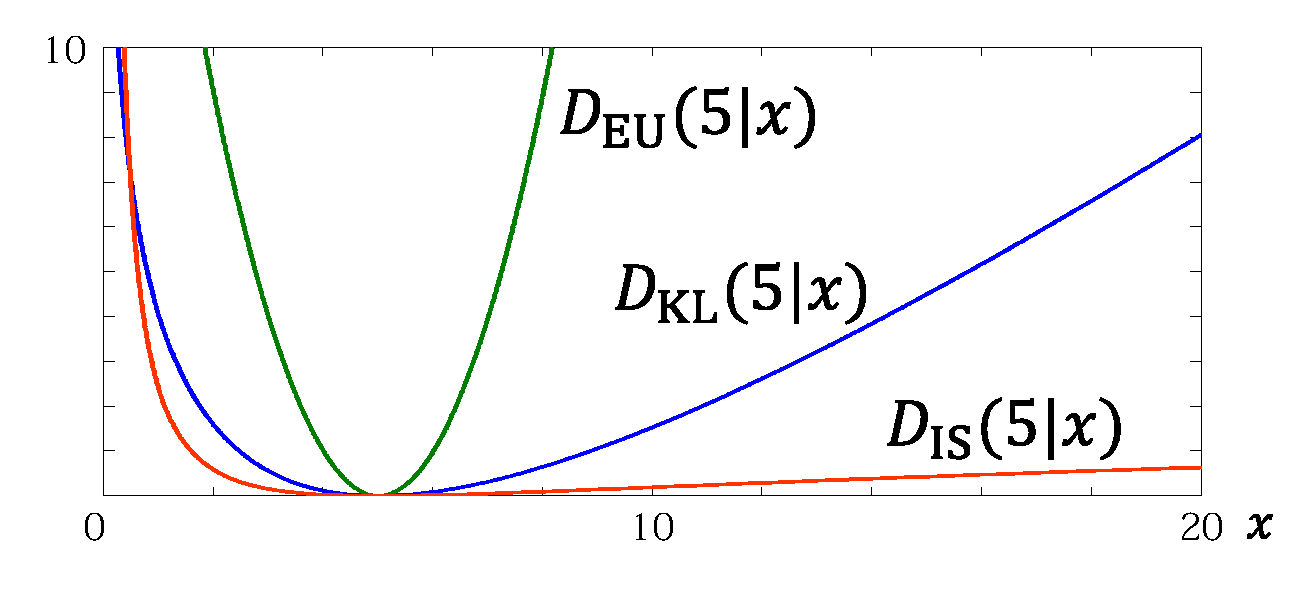
\includegraphics[width=.9\linewidth]{sections/factorization/cost_functions}
\vspace{-2mm}
\caption{ユークリッド距離,KLダイバージェンス,ISダイバージェンスに基づくコスト関数$D(5|x)$.
ユークリッド距離以外は$x=5$の左右で非対称であることに注意.}
\label{fig:cost_functions}
\end{figure}

NMFでは,観測データ$\bm{X}$が与えられたときに,
コスト関数
\begin{align}
\mathcal{D}(\bm{X}|\bm{Y}) = \sum_{n=1}^N \mathcal{D}(\bm{x}_n|\bm{y}_n)
\end{align}
を最小化する$\bm{Y}$($\bm{W}$および$\bm{H}$)を求めます.
非負値の観測ベクトル$\bm{x}_n$と非負値の再構成ベクトル$\bm{y}_n$との間の
誤差$\mathcal{D}(\bm{x}_n|\bm{y}_n)$が小さいほど,低ランク近似の精度がよいことになります.

誤差$\mathcal{D}(\bm{x}_n|\bm{y}_n)$を評価する尺度として,ユークリッド距離,
一般化Kullback-Leibler (KL) ダイバージェンス\cite{smaragdis:waspaa:2003},
およびItakura-Saito (IS) ダイバージェンス\cite{fevotte:neco:2009}などがよく利用されています.
\begin{align}
&\mathcal{D}_{\mbox{\tiny EU}}(\bm{x}_n|\bm{y}_n)
= \sum_{m=1}^M \! \left(x_{nm} - {y_{nm}}\right)^2
\!\!\!
\label{eqn:nmf_kl}
\\
&\mathcal{D}_{\mbox{\tiny KL}}(\bm{x}_n|\bm{y}_n)
= \sum_{m=1}^M \! \left(x_{nm}\log\frac{x_{nm}}{y_{nm}} - x_{nm} + {y_{nm}}\right)
\!\!\!
\label{eqn:nmf_kl}
\\
& \mathcal{D}_{\mbox{\tiny IS}}(\bm{x}_n|\bm{y}_n) 
= \sum_{m=1}^M \! \left(\frac{x_{nm}}{y_{nm}} - \log \frac{x_{nm}}{y_{nm}} - 1\right)
\!\!\!
\label{eqn:nmf_is}
\end{align}
例として,\figref{fig:cost_functions}に,
$\bm{x}_n$および$\bm{y}_n$がいずれもスカラ(1次元のベクトル)である場合のコスト関数の値を示します.
これらの関数は常に非負値をとり,$\bm{x}_n = \bm{y}_n$のときのみ0となります.

KLダイバージェンスとISダイバージェンスは,
ユークリッド距離などの通常の距離尺度と異なり,非対称性をもっています.
\begin{align}
\mathcal{D}_{\mbox{\tiny EU}}(\bm{x}_n|\bm{y}_n) &=   \mathcal{D}_{\mbox{\tiny EU}}(\bm{y}_n|\bm{x}_n)\\
\mathcal{D}_{\mbox{\tiny KL}}(\bm{x}_n|\bm{y}_n) &\ne \mathcal{D}_{\mbox{\tiny KL}}(\bm{y}_n|\bm{x}_n)\\
\mathcal{D}_{\mbox{\tiny IS}}(\bm{x}_n|\bm{y}_n) &\ne \mathcal{D}_{\mbox{\tiny IS}}(\bm{y}_n|\bm{x}_n)
\end{align}
\figref{fig:cost_functions}に示す通り,ユークリッド距離は,$x=5$の左右で対称な二次関数ですが,
KLダイバージェンスやISダイバージェンスは,$x=5$から離れるにつれて,
$x<5$よりも$x>5$の方が値の増加がはるかに緩やかな関数であることが分かります.

また,これらの中では,
ISダイバージェンスのみがスケール不変性を持っています.
すなわち,任意の実数$\alpha>0$に対して,以下が成立します.
\begin{align}
\mathcal{D}_{\mbox{\tiny EU}}(\bm{x}_n|\bm{y}_n) &\ne \mathcal{D}_{\mbox{\tiny EU}}(\alpha \bm{x}_n | \alpha \bm{y}_n)\\
\mathcal{D}_{\mbox{\tiny KL}}(\bm{x}_n|\bm{y}_n) &\ne \mathcal{D}_{\mbox{\tiny KL}}(\alpha \bm{x}_n | \alpha \bm{y}_n)\\
\mathcal{D}_{\mbox{\tiny IS}}(\bm{x}_n|\bm{y}_n) &=   \mathcal{D}_{\mbox{\tiny IS}}(\alpha \bm{x}_n | \alpha \bm{y}_n)
\end{align}
音響信号に対してNMFを適用するうえで,スケール不変性は重要な性質です.
スケール不変性を持たない場合には,
音楽音響信号全体の音量を変化させただけで,
NMFで得られる結果が異なってしまいます.
そのため,理論的にはISダイバージェンスが妥当ですが,
経験的にはKLダイバージェンスが安定してよい結果を与えることが知られています.

\subsection{乗法更新アルゴリズムに基づく最適化}
\label{sec:nmf_mu}

コスト関数$\mathcal{D}(\bm{X}|\bm{Y})$
を最小化する$\bm{Y}$を直接求めることは困難なため,
乗法更新則 (multiplicative updating rules) に基づく
反復最適化技法が提案されています\cite{kameoka:asjj:2012}.
本節では,補助関数法(付録\ref{sec:aux}節)に基づく収束性が保証された乗法更新則を紹介します.
具体的には,コスト関数$\mathcal{D}(\bm{X}|\bm{Y})$の上限関数$\mathcal{U}(\bm{X}|\bm{Y},\bm\Theta)$を設計し,
$\bm{Y}$と$\bm\Theta$について交互に逐次最小化することで,
間接的に$\mathcal{D}(\bm{X}|\bm{Y})$を逐次最小化します.
ここで,$\bm\Theta$は新たに導入された補助変数であり,
$\mathcal{U}(\bm{X}|\bm{Y},\bm\Theta)$を$\bm\Theta$について最小化することで,
もとの関数$\mathcal{D}(\bm{X}|\bm{Y})$と同じ値をとるようにしておく必要があります.
\begin{align}
\mathcal{D}(\bm{X}|\bm{Y}) = \min_{\bm\Theta} \mathcal{U}(\bm{X}|\bm{Y},\bm\Theta)
\end{align}

効率的な乗法更新則を導出するうえで,
$\mathcal{U}(\bm{X}|\bm{Y},\bm\Theta)$は,
$\bm{Y}$と$\bm\Theta$のいずれに関しても,一方が既知であれば,
もう一方に関する最小化を容易に行えることが重要です.
特に,$\bm{Y}$と$\bm\Theta$の更新則がいずれも閉形式で記述できることが理想です.
そうでないと,$\bm{Y}$と$\bm\Theta$を更新する1ステップ内においてすら,
最急降下法や(準)ニュートン法などを利用した反復最適化が必要になり,
数値的安定性・計算量・収束性などに問題が発生することがあります.

\subsection{EU-NMFの乗法更新アルゴリズム}

ユークリッド距離に基づくNMF (EU-NMF) の乗法更新則を導出します.
準備として,二次関数が下に凸であることから,
Jensenの不等式(付録\ref{sec:jensen}節)を用いて,
$f(\bm{z}) = \left(\sum_{k=1}^K z_k\right)^2$の
上限関数$u(\bm{z},\bm\lambda)$を設計します.
\begin{align}
f(\bm{z}) 
= \left(\sum_{k=1}^K \lambda_k \frac{z_k}{\lambda_k}\right)^2
\le \sum_{k=1}^K \lambda_k \left(\frac{z_k}{\lambda_k}\right)^2
= \sum_{k=1}^K \frac{z_k^2}{\lambda_k}
\overset{\mbox{\scriptsize{def}}}{=}
u(\bm{z},\bm\lambda)
\label{eqn:quad_aux}
\end{align}
ここで,$z_k \ge 0$は非負値の変数であり,
$\bm\lambda = \{\lambda_k\}_{k=1}^K$は
\begin{align}
\sum_{k=1}^K \lambda_k = 1
\label{eqn:eu_lambda_constraint}
\end{align}
を満たす非負値の補助変数です.
「和の二次関数」の上限関数として,
「二次関数の和」が得られていることに注意してください.
Jensenの不等式を用いると,和と凸関数(あるいは凹関数)の適用順序を交換できます.

等号成立条件,すなわち,
\refeq{eqn:eu_lambda_constraint}の制約条件付きで
$u(\bm{z},\bm\lambda)$を最小化する$\bm\lambda$を求めるには,
ラグランジュの未定乗数法を用います.
まず,未定乗数$\phi$を用いて,新たな関数
\begin{align}
F(\bm\lambda,\phi) = \sum_{k=1}^K \frac{z_k^2}{\lambda_k} + \phi \left(1 - \sum_{k=1}^K \lambda_k\right)
\end{align}
を考えます.ここで,$\bm\lambda$が制約条件を満たす場合には,
第二項は$0$であることに注意してください.
これを$\lambda_k$について偏微分すると
\begin{align}
\frac{\partial F(\bm\lambda,\phi)}{\partial\lambda_k} = - \frac{z_k^2}{\lambda_k^2} - \phi
\end{align}
を得ます.$\frac{\partial F(\bm\lambda,\phi)}{\partial\lambda_k} = 0$とおくと,
$\phi$を用いて$\lambda_k$が表せます.
\begin{align}
\lambda_k = \frac{z_k}{\sqrt{-\phi}}
\label{eqn:lambda_k_eu_nmf}
\end{align}
これを\refeq{eqn:eu_lambda_constraint}に代入すると,
\begin{align}
1 = \sum_{k=1}^K \lambda_k = \frac{1}{\sqrt{-\phi}}\sum_{k=1}^K z_k
\end{align}
となるので,未定乗数$\phi$は
\begin{align}
\sqrt{-\phi} = \sum_{k=1}^K z_k
\end{align}
で与えられます.これを,\refeq{eqn:lambda_k_eu_nmf}に代入すると,次式を得ます.
\begin{align}
\lambda_k = \frac{z_k}{\sum_{k=1}^K z_k}
\end{align}

この結果を用いて,コスト関数$\mathcal{D}(\bm{X}|\bm{Y})$に対して,
補助変数$\bm\lambda$を含む上限関数$\mathcal{U}(\bm{X}|\bm{Y},\bm\lambda)$を導出します.
\begin{align}
\mathcal{D}(\bm{X}|\bm{Y}) 
&= \sum_{n=1}^N \sum_{m=1}^M \left(x_{nm} - y_{nm}\right)^2
\nonumber\\
&= \sum_{n=1}^N \sum_{m=1}^M \left(x_{nm}^2 - 2 x_{nm} \sum_{k=1}^K w_{km}h_{kn} + \left(\sum_{k=1}^K w_{km} h_{kn}\right)^2\right)
\nonumber\\
&\le \sum_{n=1}^N \sum_{m=1}^M \left(x_{nm}^2 - 2 x_{nm} \sum_{k=1}^K w_{km}h_{kn} 
   + \sum_{k=1}^K \frac{w_{km}^2 h_{kn}^2}{\lambda_{nmk}}\right)
\nonumber\\
&\overset{\mbox{\scriptsize{def}}}{=} \mathcal{U}(\bm{X}|\bm{Y},\bm\lambda)
\label{eqn:eu_nmf_u}
\end{align}
ここで,\refeq{eqn:quad_aux}を用いました.
補助変数$\bm\lambda=\{\lambda_{nmk}\}_{n=1,m=1,k=1}^{N,M,K}$は,
$\sum_{k=1}^K \lambda_{nmk} = 1$を満たします.
また,等号成立条件,
すなわち$\mathcal{U}(\bm{X}|\bm{Y},\bm\lambda)$を最小化する$\bm\lambda$は次式で与えられます.
\begin{align}
\lambda_{nmk} 
= \frac{w_{km}h_{kn}}{\sum_{k'=1}^K w_{k'm}h_{k'n}}
= \frac{w_{km}h_{kn}}{y_{nm}}
\label{eqn:eu_nmf_mu_lambda}
\end{align}

最後に,\refeq{eqn:eu_nmf_u}を最小化する$\bm{Y}$($\bm{W}$および$\bm{H}$)を求めます.
まず,$\mathcal{U}(\bm{X}|\bm{Y},\bm\lambda)$を$w_{km}$について偏微分すると,
\begin{align}
\frac{\partial \mathcal{U}(\bm{X}|\bm{Y},\bm\lambda)}{\partial w_{km}} 
= \sum_{n=1}^N \left(- 2 x_{nm} h_{kn} + \frac{2 w_{km} h_{kn}^2}{\lambda_{nmk}}\right)
\end{align}
を得ます.
ここで,$\frac{\partial \mathcal{U}(\bm{X}|\bm{Y},\bm\lambda)}{\partial w_{km}}=0$とおくと,
\begin{align}
w_{km} 
= \frac{\sum_{n=1}^N x_{nm} h_{kn}}{\sum_{n=1}^N \frac{h_{kn}^2}{\lambda_{nmk}}}
\label{eqn:eu_nmf_mu_w}
\end{align}
を得ます.同様に,$\mathcal{U}(\bm{X}|\bm{Y},\bm\lambda)$を$h_{kn}$について偏微分して$0$とおくことで,
\begin{align}
h_{kn} 
= \frac{\sum_{m=1}^M x_{nm} w_{km}}{\sum_{m=1}^M \frac{w_{km}^2}{\lambda_{nmk}}}
\label{eqn:eu_nmf_mu_h}
\end{align}
を得ます.
\refeq{eqn:eu_nmf_mu_lambda},\refeq{eqn:eu_nmf_mu_w}および
\refeq{eqn:eu_nmf_mu_h}は互いに依存関係にあり,
$\mathcal{U}(\bm{X}|\bm{Y},\bm\lambda)$を最小化する$\bm\lambda$,$\bm{W}$および$\bm{H}$を
一挙に求めることができません.
そのため,これらの式を交互に反復計算することにより,
徐々に\refeq{eqn:eu_nmf_u}を小さくしていくことになります.

NMFの乗法更新則は,補助変数を介さずに表現することもできます.
具体的には,\refeq{eqn:eu_nmf_mu_lambda}を\refeq{eqn:eu_nmf_mu_w}および
\refeq{eqn:eu_nmf_mu_h}に代入することで,
\begin{align}
&w_{km} 
\gets \frac{\sum_{n=1}^N x_{nm} h_{kn}}{\sum_{n=1}^N \frac{h_{kn}^2}{\lambda_{nmk}}}
= \frac{\sum_{n=1}^N x_{nm} h_{kn}}{\sum_{n=1}^N \frac{y_{nm} h_{kn}}{w_{km}}}
= \frac{\sum_{n=1}^N x_{nm} h_{kn}}{\sum_{n=1}^N y_{nm} h_{kn}} w_{km}
\label{eqn:eu_nmf_mu_w2}
\\
& h_{kn}
\gets \frac{\sum_{m=1}^M x_{nm} w_{km}}{\sum_{m=1}^M \frac{w_{km}^2}{\lambda_{nmk}}}
%= \frac{\sum_{m=1}^M x_{nm} w_{km}}{\sum_{m=1}^M \frac{y_{nm} w_{km}}{h_{kn}}}
= \frac{\sum_{m=1}^M x_{nm} w_{km}}{\sum_{m=1}^M y_{nm} w_{km}} h_{kn}
\label{eqn:eu_nmf_mu_h2}
\end{align}
を得ます.
ここで,記号$\gets$は,右辺値を左辺値に代入して更新するという意味です.
$\gets$の右側においては,
$\bm\lambda$,$\bm{W}$および$\bm{H}$の更新前の古い値を用います.
同じ変数が$\gets$の左右に登場すると混乱するため,
等号ではなく,記号$\gets$を用いています.

これらが「乗法」更新則と呼ばれる所以は,
自分自身に係数を掛け合わせて更新を行うからです.
例えば,\refeq{eqn:eu_nmf_mu_w2}では,
$w_{km}$に係数$\frac{\sum_{n=1}^N x_{nm} h_{kn}}{\sum_{n=1}^N y_{nm} h_{kn}} \ge 0 $を掛け合わせています.
このとき,係数も非負値であることから,特別な制約を導入しなくても,
$w_{km}$の非負値性は自然に保たれます.
また,$w_{km}=0$として初期化すると,
以降の更新では常に$w_{km}=0$が維持されます.

\refeq{eqn:eu_nmf_mu_w2}および\refeq{eqn:eu_nmf_mu_h2}は,
行列演算を用いて簡潔に書けます.
\begin{align}
\bm{W} \gets \frac{\bm{H}\bm{X}^T}{\bm{H}\bm{Y}^T} \odot \bm{W}
\label{eqn:eu_nmf_mu_W}
\\
\bm{H} \gets \frac{\bm{W}\bm{X}}{\bm{W}\bm{Y}} \odot \bm{H}
\label{eqn:eu_nmf_mu_H}
\end{align}
ここで,割り算---や掛け算$\odot$は行列の各要素ごとに行うものとします.
高速な行列演算が可能なプログラミング言語(例:MATLAB)では,
for文を使わずに上記の更新式を直接コーディングすることができ,
CPUやGPUのベクトル演算機能を利用した高速な更新が可能になります.

\refalgo{algo:eu-nmf-ml}に,EU-NMFのアルゴリズムを示します
(これが実は,ある確率モデルの最尤推定になっていることはあとで示します).
このアルゴリズムは山登り法(NMFではコスト関数を最小化しているので実際には「山下り法」)の一種であり,
大域的な最適解を見つけられる保証はなく,
得られる結果は$\bm{W}$および$\bm{H}$の初期値に大きな影響を受けます.
また,スケールの任意性を解消するため,
$\sum_{m=1}^M w_{km} = 1$を満たすように正規化しておくことにします.
具体的には,$w_{km}$を更新した結果,$\sum_{m=1}^M w_{km} = s$になってしまったとすると,
すべての$m,n$について$w_{km} \gets \frac{1}{s} w_{km}$および
$h_{kn} \gets s h_{kn}$と更新しておきます.
この処理ではコスト関数の値は変化しません.
$\sum_{n=1}^N h_{kn} = 1$となるようアクティベーションを正規化することもできますが,
基底ベクトルを正規化しておくのが一般的です.
\begin{algobox}{EU-NMFの最尤推定}
\label{algo:eu-nmf-ml}
\begin{algorithmic}[1]
\Require 非負値行列$\bm{X} \in \mathbb{R}_+^{M \times N}$, 基底数$K$
\State 非負値行列$\bm{W} \in \mathbb{R}_+^{M \times K}$をランダムに初期化
\State 非負値行列$\bm{H} \in \mathbb{R}_+^{M \times K}$をランダムに初期化
\While{上限関数$\mathcal{U}(\bm{X}|\bm{Y},\bm\lambda)$が未収束}
\State $\displaystyle \bm{W} \gets \frac{\bm{H}\bm{X}^T}{\bm{H}\bm{Y}^T} \odot \bm{W}$ 
\State $\displaystyle \bm{H} \gets \frac{\bm{W}\bm{X}}{\bm{W}\bm{Y}} \odot \bm{H}$ 
\EndWhile\\
{\bf Return} 非負値行列$\bm{W}$, $\bm{H}$
\end{algorithmic}
\end{algobox}

\subsection{KL-NMFの乗法更新アルゴリズム}

EU-NMFとほとんど同様の方法で,
KLダイバージェンスに基づくNMF (KL-NMF) の乗法更新則を導出することができます.
準備として,負の対数関数が下に凸であることから,
Jensenの不等式(付録\ref{sec:jensen}節)を用いて,
$f(\bm{z}) = - \log \left(\sum_{k=1}^K z_k \right)$の
上限関数$u(\bm{z},\bm\lambda)$を設計します.
\begin{align}
f(\bm{z})
= - \log \left(\sum_{k=1}^K \lambda_k \frac{z_k}{\lambda_k}\right)
\le - \sum_{k=1}^K \lambda_k \log \frac{z_k}{\lambda_k}
\overset{\mbox{\scriptsize{def}}}{=}
u(\bm{z},\bm\lambda)
\label{eqn:log_aux}
\end{align}
ここで,$z_k \ge 0$は非負値の変数であり,
$\bm\lambda = \{\lambda_k\}_{k=1}^K$は
\begin{align}
\sum_{k=1}^K \lambda_k = 1
\label{eqn:kl_lambda_constraint}
\end{align}
を満たす非負値の補助変数です.
「和の対数関数」の上限関数として,
「対数関数の和」が得られていることに注意してください.

等号成立条件,すなわち,
\refeq{eqn:kl_lambda_constraint}の制約条件付きで
$u(\bm{z},\bm\lambda)$を最小化する$\bm\lambda$を求めるには,
ラグランジュの未定乗数$\phi$を用いて,新たな関数
\begin{align}
F(\bm\lambda,\phi) = \sum_{k=1}^K \lambda_k \log \frac{z_k}{\lambda_k} + \phi \left(1 - \sum_{k=1}^K \lambda_k\right)
\end{align}
を考えます.これを$\lambda_k$について偏微分すると
\begin{align}
\frac{\partial F(\bm\lambda,\phi)}{\partial\lambda_k} 
= \log z_k - \log \lambda_k - 1 - \phi
\end{align}
を得ます.$\frac{\partial F(\bm\lambda,\phi)}{\partial\lambda_k} = 0$とおくと,
$\phi$を用いて$\lambda_k$が表せます.
\begin{align}
\lambda_k = \frac{z_k}{e^{1+\phi}}
\label{eqn:lambda_k_kl_nmf}
\end{align}
これを\refeq{eqn:kl_lambda_constraint}に代入すると,
\begin{align}
1 = \sum_{k=1}^K \lambda_k = \frac{1}{e^{1+\phi}}\sum_{k=1}^K z_k
\end{align}
となるので,未定乗数$\phi$は
\begin{align}
e^{1+\phi} = \sum_{k=1}^K z_k
\end{align}
で与えられます.これを,\refeq{eqn:lambda_k_kl_nmf}に代入すると,次式を得ます.
\begin{align}
\lambda_k = \frac{z_k}{\sum_{k=1}^K z_k}
\end{align}

この結果を用いて,コスト関数$\mathcal{D}(\bm{X}|\bm{Y})$に対して,
補助変数$\bm\lambda$を含む上限関数$\mathcal{U}(\bm{X}|\bm{Y},\bm\lambda)$を導出します.
\begin{align}
\mathcal{D}(\bm{X}|\bm{Y}) 
&= \sum_{n=1}^N \sum_{m=1}^M \left(x_{nm} \log x_{nm} - x_{nm} \log y_{nm} - x_{nm} + y_{nm}\right)
\nonumber\\
&\overset{c}{=} \sum_{n=1}^N \sum_{m=1}^M \left(- x_{nm} \log \sum_{k=1}^K w_{km}h_{kn} + \sum_{k=1}^K w_{km}h_{kn}\right)
\nonumber\\
&\le \sum_{n=1}^N \sum_{m=1}^M \left(- x_{nm} \sum_{k=1}^K \lambda_{nmk} \log \frac{w_{km}h_{kn}}{\lambda_{nmk}} + \sum_{k=1}^K w_{km}h_{kn}\right)
\nonumber\\
&\overset{\mbox{\scriptsize{def}}}{=} \mathcal{U}(\bm{X}|\bm{Y},\bm\lambda)
\label{eqn:kl_nmf_u}
\end{align}
ここで,
%定数項を除いて等しいことを表す記号$\overset{c}{=}$を導入し
%(観測データ$x_{nm}$は既知なので定数項),
\refeq{eqn:log_aux}を用いました.
また,補助変数$\bm\lambda$は,
$\sum_{k=1}^K \lambda_{nmk} = 1$を満たすものとします.
等号成立条件,
すなわち$\mathcal{U}(\bm{X}|\bm{Y},\bm\lambda)$を最小化する$\bm\lambda$は次式で与えられます.
\begin{align}
\lambda_{nmk} 
= \frac{w_{km}h_{kn}}{\sum_{k'=1}^K w_{k'm}h_{k'n}}
= \frac{w_{km}h_{kn}}{y_{nm}}
\label{eqn:kl_nmf_mu_lambda}
\end{align}

最後に,\refeq{eqn:kl_nmf_u}を最小化する$\bm{Y}$($\bm{W}$および$\bm{H}$)を求めます.
まず,$\mathcal{U}(\bm{X}|\bm{Y},\bm\lambda)$を$w_{km}$について偏微分すると,
\begin{align}
\frac{\partial \mathcal{U}(\bm{X}|\bm{Y},\bm\lambda)}{\partial w_{km}} 
= \sum_{n=1}^N \left(- \frac{x_{nm} \lambda_{nmk}}{w_{km}} + h_{kn} \right)
\end{align}
を得ます.
ここで,$\frac{\partial \mathcal{U}(\bm{X}|\bm{Y},\bm\lambda)}{\partial w_{km}}=0$とおくと,
\begin{align}
w_{km} 
= \frac{\sum_{n=1}^N x_{nm} \lambda_{nmk}}{\sum_{n=1}^N h_{kn}}
\label{eqn:kl_nmf_mu_w}
\end{align}
を得ます.同様に,$\mathcal{U}(\bm{X}|\bm{Y},\bm\lambda)$を$h_{kn}$について偏微分して$0$とおくことで,
\begin{align}
h_{kn} 
= \frac{\sum_{m=1}^M x_{nm} \lambda_{nmk}}{\sum_{m=1}^M w_{km}}
\label{eqn:kl_nmf_mu_h}
\end{align}
を得ます.
EU-NMFと同様に,
\refeq{eqn:kl_nmf_mu_lambda},\refeq{eqn:kl_nmf_mu_w}および\refeq{eqn:kl_nmf_mu_h}
を反復することにより,
$\mathcal{U}(\bm{X}|\bm{Y},\bm\lambda)$を逐次最小化していくことができます.

補助変数を介さない乗法更新則は,
\refeq{eqn:kl_nmf_mu_lambda}を\refeq{eqn:kl_nmf_mu_w}および\refeq{eqn:kl_nmf_mu_h}
に代入することで得られます.
\begin{align}
w_{km} 
&\gets \frac{\sum_{n=1}^N x_{nm} \frac{w_{km} h_{kn}}{y_{nm}}}{\sum_{n=1}^N h_{kn}}
= \frac{\sum_{n=1}^N h_{kn} \frac{x_{nm}}{y_{nm}}}{\sum_{n=1}^N h_{kn}} w_{km}
\label{eqn:kl_nmf_mu_w2}
\\
h_{kn} 
&\gets \frac{\sum_{m=1}^M x_{nm} \frac{w_{km} w_{km}}{y_{nm}}}{\sum_{m=1}^M w_{km}}
= \frac{\sum_{m=1}^M w_{km} \frac{x_{nm}}{y_{nm}}}{\sum_{m=1}^M w_{kn}} h_{kn}
\label{eqn:kl_nmf_mu_h2}
\end{align}
全要素が$1$の行列を$\bm{1} \in \mathbb{R}^{M \times N}$とすると,
行列演算として記述できます.
\begin{align}
\bm{W} \gets \frac{\bm{H} \frac{\bm{X}^T}{\bm{Y}^T}}{\bm{H}\bm{1}^T} \odot \bm{W}
\label{eqn:kl_nmf_mu_W}
\\
\bm{H} \gets \frac{\bm{W} \frac{\bm{X}}{\bm{Y}}}{\bm{W}\bm{1}} \odot \bm{H}
\label{eqn:kl_nmf_mu_H}
\end{align}

\begin{algobox}{KL-NMFの最尤推定}
\label{algo:kl-nmf-ml}
\begin{algorithmic}[1]
\Require 非負値行列$\bm{X} \in \mathbb{R}_+^{M \times N}$, 基底数$K$
\State 非負値行列$\bm{W} \in \mathbb{R}_+^{M \times K}$をランダムに初期化
\State 非負値行列$\bm{H} \in \mathbb{R}_+^{M \times K}$をランダムに初期化
\While{上限関数$\mathcal{U}(\bm{X}|\bm{Y},\bm\lambda)$が未収束}
\State $\displaystyle \bm{W} \gets \frac{\bm{H} \frac{\bm{X}^T}{\bm{Y}^T}}{\bm{H}\bm{1}^T} \odot \bm{W}$ 
\State $\displaystyle \bm{H} \gets \frac{\bm{W} \frac{\bm{X}}{\bm{Y}}}{\bm{W}\bm{1}} \odot \bm{H}$ 
\EndWhile\\
{\bf Return} 非負値行列$\bm{W}$, $\bm{H}$
\end{algorithmic}
\end{algobox}
\refalgo{algo:kl-nmf-ml}に,KL-NMFのアルゴリズムを示します.
これも,EU-NMFと同様に,ある確率モデルの最尤推定としての解釈が可能です.

\subsection{IS-NMFの乗法更新アルゴリズム}

ISダイバージェンスに基づくNMF (IS-NMF) の乗法更新則を導出します.
準備として,逆数関数が下に凸であることから,
Jensenの不等式(付録\ref{sec:jensen}節)を用いて,
$f(\bm{z})=\frac{1}{\left(\sum_{k=1}^K z_k \right)}$
の上限関数$u(\bm{z},\bm\lambda)$を設計します.
\begin{align}
f(\bm{z}) 
= \frac{1}{\left(\sum_{k=1}^K \lambda_k \frac{z_k}{\lambda_k} \right)}
\le \sum_{k=1}^K \lambda_k \frac{1}{\frac{z_k}{\lambda_k}}
= \sum_{k=1}^K \lambda_k^2 \frac{1}{z_k}
\overset{\mbox{\scriptsize{def}}}{=}
u(\bm{z},\bm\lambda)
\label{eqn:inv_aux}
\end{align}
ここで,$z_k \ge 0$は非負値の変数であり,
$\bm\lambda = \{\lambda_k\}_{k=1}^K$は
\begin{align}
\sum_{k=1}^K \lambda_k = 1
\label{eqn:is_lambda_constraint}
\end{align}
を満たす非負値の補助変数です.
「和の逆数関数」の上限関数として,
「逆数関数の和」が得られていることに注意してください.

等号成立条件,すなわち,
\refeq{eqn:is_lambda_constraint}の制約条件付きで
$u(\bm{z},\bm\lambda)$を最小化する$\bm\lambda$を求めるには,
未定乗数$\phi$を用いて,新たな関数
\begin{align}
F(\bm\lambda,\phi) = \sum_{k=1}^K \lambda_k^2 \frac{1}{z_k} + \phi \left(1 - \sum_{k=1}^K \lambda_k\right)
\end{align}
を考えます.これを$\lambda_k$について偏微分すると
\begin{align}
\frac{\partial F(\bm\lambda,\phi)}{\partial\lambda_k} 
= \frac{2 \lambda_k}{z_k} - \phi
\end{align}
を得ます.$\frac{\partial F(\bm\lambda,\phi)}{\partial\lambda_k} = 0$とおくと,
$\phi$を用いて$\lambda_k$が表せます.
\begin{align}
\lambda_k = \frac{\phi}{2} z_k
\label{eqn:lambda_k_is_nmf}
\end{align}
これを\refeq{eqn:is_lambda_constraint}に代入すると,
\begin{align}
1 = \sum_{k=1}^K \lambda_k = \frac{\phi}{2}\sum_{k=1}^K z_k
\end{align}
となるので,未定乗数$\phi$は
\begin{align}
\frac{2}{\phi} = \sum_{k=1}^K z_k
\end{align}
で与えられます.これを,\refeq{eqn:lambda_k_is_nmf}に代入すると,次式を得ます.
\begin{align}
\lambda_k = \frac{z_k}{\sum_{k=1}^K z_k}
\end{align}

さらに,対数関数$f(z)=\log(z)$の上限関数$u(z,\omega)$を設計します.
対数関数は上に凸であることから,任意の点$\omega > 0$における接線は
常に対数関数の上側にあります.
したがって,$\omega$における一次のテイラー展開を行うと,
\begin{align}
f(z) \le \log \omega + \frac{z}{\omega} - 1
\overset{\mbox{\scriptsize{def}}}{=}
u(z,\omega)
\label{eqn:log_tangent_aux}
\end{align}
を得ます.
等号成立条件,すなわち,
$u(z,\omega)$を最小化する$\omega$は,
$u(z,\omega)$を$\omega$で偏微分して$0$とおくことで求まります.
\begin{align}
 \omega = x
\end{align}

これらの結果を用いて,コスト関数$\mathcal{D}(\bm{X}|\bm{Y})$に対して,
補助変数$\bm\lambda$および$\bm\omega$を含む上限関数$\mathcal{U}(\bm{X}|\bm{Y},\bm\lambda,\bm\omega)$を導出します.
\begin{align}
\mathcal{D}(\bm{X}|\bm{Y}) 
&= \sum_{n=1}^N \sum_{m=1}^M \left(\frac{x_{nm}}{y_{nm}} - \log \frac{x_{nm}}{y_{nm}} - 1\right)
\nonumber\\
&= \sum_{m=1}^M \left(\frac{x_{nm}}{\sum_{k=1}^K w_{km} h_{kn}} - \log \frac{x_{nm}}{\sum_{k=1}^K w_{km} h_{kn}} - 1\right)
\nonumber\\
&\overset{c}{=}  \sum_{m=1}^M \left(\frac{x_{nm}}{\sum_{k=1}^K w_{km} h_{kn}} + \log \sum_{k=1}^K w_{km} h_{kn} \right)
\nonumber\\
&\le \sum_{n=1}^N \sum_{m=1}^M \left(\sum_{k=1}^K \frac{x_{nm} \lambda_{nmk}^2}{w_{km} h_{kn}} 
+ \log \omega_{nm} + \frac{1}{\omega_{nm}}\sum_{k=1}^K w_{km} h_{kn} - 1\right)
\nonumber\\
&\overset{\mbox{\scriptsize{def}}}{=} \mathcal{U}(\bm{X}|\bm{Y},\bm\lambda,\bm\omega)
\label{eqn:is_nmf_u}
\end{align}
ここで,\refeq{eqn:inv_aux}および\refeq{eqn:log_tangent_aux}を用いました.
補助変数に関しては,$\bm\lambda=\{\lambda_{nmk}\}_{n=1,m=1,k=1}^{N,M,K}$は
$\sum_{k=1}^K \lambda_{nmk} = 1$を満たし,
$\bm\omega=\{\omega_{nm}\}_{n=1,m=1}^{N,M}$はすべて非負値とします.
等号成立条件,
すなわち$\mathcal{U}(\bm{X}|\bm{Y},\bm\lambda,\bm\omega)$を最小化する$\bm\lambda$および$\bm\omega$は次式で与えられます.
\begin{align}
\lambda_{nmk} 
&= \frac{w_{km}h_{kn}}{\sum_{k'=1}^K w_{k'm}h_{k'n}}
= \frac{w_{km}h_{kn}}{y_{nm}}
\label{eqn:is_nmf_mu_lambda}
\\
\omega_{nm} 
&= \sum_{k=1}^K w_{km} h_{kn} = y_{nm}
\label{eqn:is_nmf_mu_omega}
\end{align}

最後に,\refeq{eqn:is_nmf_u}を最小化する$\bm{Y}$($\bm{W}$および$\bm{H}$)を求めます.
まず,$\mathcal{U}(\bm{X}|\bm{Y},\bm\lambda,\bm\omega)$を$w_{km}$について偏微分すると,
\begin{align}
\frac{\partial \mathcal{U}(\bm{X}|\bm{Y},\bm\lambda,\bm\omega)}{\partial w_{km}} 
= \sum_{n=1}^N \left(- \frac{x_{nm}\lambda_{nmk}^2}{w_{km}^2 h_{kn}} + \frac{h_{kn}}{\omega_{nm}}\right)
\end{align}
を得ます.
ここで,$\frac{\partial \mathcal{U}(\bm{X}|\bm{Y},\bm\lambda.\bm\omega)}{\partial w_{km}}=0$とおくと,
\begin{align}
w_{km} 
= \sqrt{
       \frac{\sum_{n=1}^N \frac{x_{nm} \lambda_{nmk}^2}{h_{kn}}}
       {\sum_{n=1}^N \frac{h_{kn}}{\omega_{nm}}}
  }
\label{eqn:is_nmf_mu_w}
\end{align}
を得ます.同様に,$\mathcal{U}(\bm{X}|\bm{Y},\bm\lambda,\bm\omega)$を$h_{kn}$について偏微分して$0$とおくと,
\begin{align}
h_{kn} 
= \sqrt{
  \frac{\sum_{m=1}^M \frac{x_{nm} \lambda_{nmk}^2}{w_{km}}}
       {\sum_{n=1}^N \frac{h_{kn}}{\omega_{nm}}}
  }
\label{eqn:is_nmf_mu_h}
\end{align}
を得ます.
\refeq{eqn:is_nmf_mu_lambda},\refeq{eqn:is_nmf_mu_omega},\refeq{eqn:is_nmf_mu_w}および\refeq{eqn:is_nmf_mu_h}
を反復することにより,
$\mathcal{U}(\bm{X}|\bm{Y},\bm\lambda,\bm\omega)$を逐次最小化していくことができます.

補助変数を介さない乗法更新則は,
\refeq{eqn:is_nmf_mu_lambda}および\refeq{eqn:is_nmf_mu_omega}を,
\refeq{eqn:is_nmf_mu_w}および\refeq{eqn:is_nmf_mu_h}に代入することで得られます.
\begin{align}
w_{km} 
&\gets 
\sqrt{
       \frac{\sum_{n=1}^N \frac{x_{nm} w_{km}^2 h_{kn}^2}{h_{kn} y_{nm}^2}}
       {\sum_{n=1}^N \frac{h_{kn}}{y_{nm}}}
  }
=
\sqrt{
       \frac{\sum_{n=1}^N h_{kn} \frac{x_{nm}}{y_{nm}^2}}
       {\sum_{n=1}^N h_{kn} \frac{1}{y_{nm}}}
  } w_{km}
\label{eqn:is_nmf_mu_w2}
\\
h_{kn} 
&\gets 
\sqrt{
       \frac{\sum_{m=1}^M \frac{x_{nm} w_{km}^2 h_{kn}^2}{w_{km} y_{nm}^2}}
       {\sum_{m=1}^M \frac{w_{km}}{y_{nm}}}
  }
=
\sqrt{
       \frac{\sum_{m=1}^M w_{kn} \frac{x_{nm}}{y_{nm}^2}}
       {\sum_{m=1}^M w_{km} \frac{1}{y_{nm}}}
  } h_{kn}
\label{eqn:is_nmf_mu_h2}
\end{align}
さらに,これらは行列演算として簡潔に記述することもできます.
\begin{align}
\bm{W} \gets \sqrt{\frac{\bm{H} \frac{\bm{X}^T}{\bm{Y}^T \odot \bm{Y}^T}} {\bm{H}\frac{\bm{1}^T}{\bm{Y}^T}}} \odot \bm{W}
\label{eqn:is_nmf_mu_W}
\\
\bm{H} \gets \sqrt{\frac{\bm{W} \frac{\bm{X}}{\bm{Y} \odot \bm{Y}}} {\bm{W}\frac{\bm{1}}{\bm{Y}}}} \odot \bm{H}
\label{eqn:is_nmf_mu_H}
\end{align}
ここで,$\bm{1} \in \mathbb{R}^{M \times N}$は,全ての要素が$1$の行列です.
$\sqrt{\ \ \ }$は行列の要素ごとに平方根をとるものとします.

\refalgo{algo:is-nmf-ml}に,IS-NMFのアルゴリズムを示します.
IS-NMFも,ある確率モデルの最尤推定としての解釈が可能です.
\refalgo{algo:eu-nmf-ml},\refalgo{algo:kl-nmf-ml},\refalgo{algo:is-nmf-ml}を比較すると,
EU-NMFでは,分子・分母に$\bm{X}$および$\bm{Y}$を,
KL-NMFでは$\frac{\bm{X}}{\bm{Y}}$および$\bm{1}$を,
IS-NMFでは$\frac{\bm{X}}{\bm{Y}\odot\bm{Y}}$および$\frac{\bm{1}}{\bm{Y}}$をそれぞれ掛けています
(比はすべて$\frac{\bm{X}}{\bm{Y}}$で等しい).
NMFには$\bm{W}$や$\bm{H}$をスパースに誘導する効果があり,
それらの積で計算できる再構成行列$\bm{Y}=\bm{W}\bm{H}$もスパースになりやすい傾向があります.
このとき,$\bm{Y}$のある要素が非常に小さな値になると,
その逆数は非常に大きな値となってしまうため,IS-NMFは数値的に不安定になることがあります.

\begin{algobox}{IS-NMFの最尤推定}
\label{algo:is-nmf-ml}
\begin{algorithmic}[1]
\Require 非負値行列$\bm{X} \in \mathbb{R}_+^{M \times N}$, 基底数$K$
\State 非負値行列$\bm{W} \in \mathbb{R}_+^{M \times K}$をランダムに初期化
\State 非負値行列$\bm{H} \in \mathbb{R}_+^{M \times K}$をランダムに初期化
\While{上限関数$\mathcal{U}(\bm{X}|\bm{Y},\bm\lambda,\bm\omega)$が未収束}
\State $\displaystyle \bm{W} \gets \sqrt{\frac{\bm{H} \frac{\bm{X}^T}{\bm{Y}^T \odot \bm{Y}^T}} {\bm{H}\frac{\bm{1}^T}{\bm{Y}^T}}} \odot \bm{W}$ 
\State $\displaystyle \bm{H} \gets \sqrt{\frac{\bm{W} \frac{\bm{X}}{\bm{Y} \odot \bm{Y}}} {\bm{W}\frac{\bm{1}}{\bm{Y}}}} \odot \bm{H}$ 
\EndWhile\\
{\bf Return} 非負値行列$\bm{W}$, $\bm{H}$
\end{algorithmic}
\end{algobox}

\subsection{$\bm\beta$-NMFの乗法更新アルゴリズム}

これまで議論してきたEU-NMF,KL-NMF,IS-NMFを統一的に取り扱うことができるNMFとして,
$\beta$ダイバージェンスに基づく$\beta$-NMFが提案されています\cite{nakano:mlsp:2010}.
観測ベクトル$\bm{x}_n$と再構成ベクトル$\bm{y}_n$との近似誤差を表す
$\beta$ダイバージェンスは次式で定義されます.
\begin{align}
\mathcal{D}_\beta(\bm{x}_n | \bm{y}_n) 
=
\sum_{m=1}^M \left(
\frac{x_{nm}^\beta}{\beta(\beta - 1)} 
+ \frac{y_{nm}^\beta}{\beta} 
- \frac{x_{nm} y_{nm}^{\beta - 1}}{\beta - 1}
\right)
\label{eqn:beta_div}
\end{align}
ここで,$\beta \in \mathbb{R}$は$0,1$を除く任意の実数であり,
$\beta=2$のときユークリッド距離に一致します.
また,$\beta \rightarrow 1$および$\beta \rightarrow 0$の極限を考えると,
\begin{align}
\lim_{\beta \rightarrow 1} \mathcal{D}_\beta(\bm{x}_n | \bm{y}_n)
&= 
\lim_{\beta \rightarrow 1}
\sum_{m = 1}^N 
\left(x_{nm} \frac{x_{nm}^{\beta - 1} - y_{nm}^{\beta - 1}}{1 - \beta} 
      - \frac{x_{nm}^\beta - y_{nm}^\beta}{\beta}\right)
\nonumber\\
&= 
\sum_{m = 1}^N
\left(
x_{nm}(\log x_{nm} - \log y_{nm}) - (x_{nm} - y_{nm})
\right)
\\
\lim_{\beta \rightarrow 0} \mathcal{D}_\beta(\bm{x}_n | \bm{y}_n)
&= 
\lim_{\beta \rightarrow 0}
\sum_{m = 1}^N 
\left(x_{nm} \frac{y_{nm}^{\beta - 1}}{1 - \beta} - \frac{x_{nm}^\beta - y_{nm}^\beta}{\beta}
      + \frac{x_{nm}^\beta}{\beta - 1}\right)
\nonumber\\
&= 
\sum_{m = 1}^N
\left(
\frac{x_{nm}}{y_{nm}} - \log \frac{x_{nm}}{y_{nm}} - 1
\right)
\end{align}
となるので,$\beta \rightarrow 1$のときKLダイバージェンス,
$\beta \rightarrow 0$のときISダイバージェンスと等価であることが分かります.
このように,$\beta$の値を調節することで,
EU-NMF,KL-NMF,IS-NMFをはじめ,それらの中間的な性質をもつNMFを統一的に記述できます.

$\beta$ダイバージェンスに基づくNMF ($\beta$-NMF) の乗法更新則を導出しましょう.
\refeq{eqn:beta_div}で与えられるコスト関数をみると,
第一項は定数ですが,第二項および第三項は,$\beta$の値によって
下に凸であるか上に凸であるかが決まります.
そのため,$\beta$の値で場合分けを行う必要があります.

\begin{figure}[t]
\centering
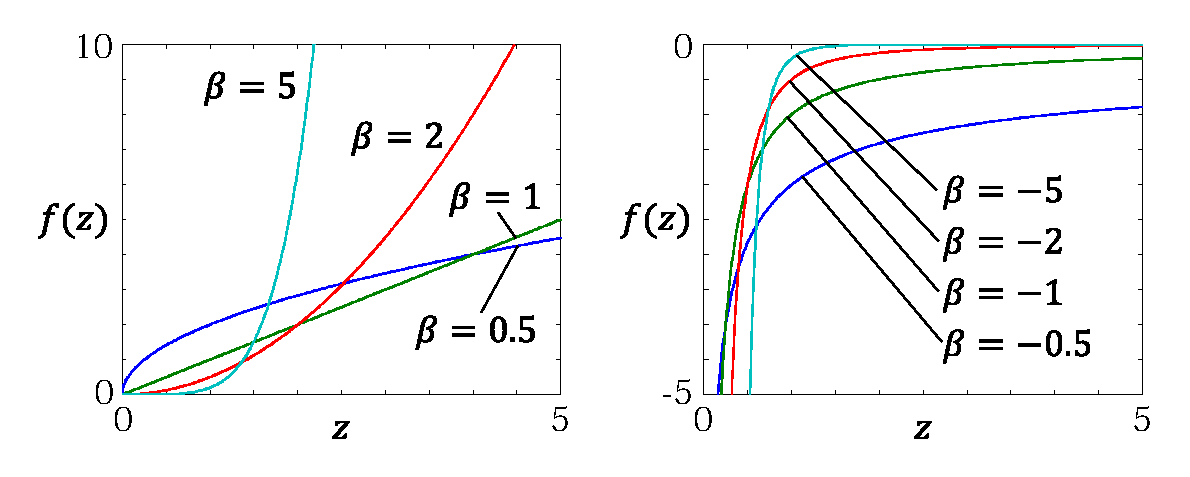
\includegraphics[width=.99\linewidth]{sections/factorization/beta_div_aux_functions}
\caption{いくつかの$\beta$に対する関数$f_\beta(z)=\frac{1}{\beta} z^\beta$のプロット.
$\beta=1$を境界として,$\beta \ge 1$のときは下に凸 (convex),$\beta \le 1$のときは上に凸 (concave) となることに注意.}
\label{fig:beta_div_aux_functions}
\end{figure}

まず,準備として,
関数$f_\beta(z)=\frac{1}{\beta} z^\beta \ (z > 0)$について考えます(\figref{fig:beta_div_aux_functions}).
$\beta \le 1$の場合は,$f_\beta(z)$は上に凸であることから,
任意の点$\omega > 0$における一次のテイラー展開
($\omega$における接線方程式)を考えることで,
$f_\beta(z)$の上限関数$u_\beta(z,\omega)$を設計できます.
\begin{align}
f_\beta(z)
\le
\frac{1}{\beta} \omega^\beta + \omega^{\beta - 1}\left(z - \omega\right)
=
\frac{\beta + 1}{\beta} \omega^\beta + \omega^{\beta - 1} z
\overset{\mbox{\scriptsize{def}}}{=}
u_\beta(z,\omega)
\end{align}
ここで,等号成立条件,すなわち,$u_\beta(z,\omega)$を最小化する$\omega$は,
$u_\beta(z,\omega)$を$\omega$で偏微分して$0$とおくことで求まります
(導出はEU-NMF, KL-NMF, IS-NMFなどと同様なので省略).
\begin{align}
\omega = x
\end{align}
一方,$\beta \ge 1$の場合は,$f_\beta(z)$は下に凸であることから,
Jensenの不等式を用いて,$f'_\beta(\bm{z}) = \frac{1}{\beta} \left(\sum_{k=1}^K z_k\right)^\beta$の
上限関数$u'_\beta(\bm{z},\bm\lambda)$を設計できます.
\begin{align}
f'_\beta(\bm{z}) 
= 
\frac{1}{\beta} \left(\sum_{k=1}^K \lambda_k \frac{z_k}{\lambda_k}\right)^\beta
\le 
\frac{1}{\beta} \sum_{k=1}^K \lambda_k \left(\frac{z_k}{\lambda_k}\right)^\beta
\overset{\mbox{\scriptsize{def}}}{=}
u'_\beta(\bm{z},\bm\lambda)
\end{align}
ここで,補助変数$\bm\lambda = \{\lambda_k\}_{k=1}^K$は,$\sum_{k=1}^K \lambda_k = 1$を満たします.
等号成立条件,すなわち,$u'_\beta(\bm{z},\bm\lambda)$を最小化する$\bm\lambda$は,
$u'_\beta(\bm{z},\bm\lambda)$を$\bm\lambda$で偏微分して$0$とおくことで求まります(導出は省略).
\begin{align}
\lambda_k = \frac{z_k}{\sum_{k=1}^K z_k}
\end{align}

また,関数$g'_\beta(\bm{z})
= - \frac{1}{\beta - 1} \left(\sum_{k=1}^K z_k\right)^{\beta - 1}$
および関数$g_\beta(z) = - \frac{1}{\beta - 1} z^{\beta - 1}$についても,
$g'_\beta(\bm{z}) = - f'_{\beta-1}(\bm{z})$
および$g_\beta(z) = - f_{\beta-1}(z)$となることを用いて,
上限関数をそれぞれ設計できます.
\begin{align}
g'_\beta(\bm{z}) &\le - u'_{\beta - 1}(\bm{z},\bm\lambda)
&(\beta \le 2)
\\
g_\beta(z) &\le - u_{\beta - 1}(z,\omega)
&(\beta \ge 2)
\end{align}
各場合における等号成立条件,すなわち,上限関数を最小化する
補助変数$\bm\lambda$あるいは$\omega$は,次式で与えられます.
\begin{align}
\lambda_k &= \frac{z_k}{\sum_{k=1}^K z_k} &(\beta \le 2)
\\
\omega &= x &(\beta \ge 2)
\end{align}

これらの結果を用いて,コスト関数$\mathcal{D}(\bm{X}|\bm{Y})$に対して,
補助変数$\bm\lambda$および$\bm\omega$を含む
上限関数$\mathcal{U}(\bm{X}|\bm{Y},\bm\lambda,\bm\omega)$を導出します.
\begin{align}
&\mathcal{D}(\bm{X}|\bm{Y}) 
\overset{c}{=}
\sum_{n=1}^N \sum_{m=1}^M 
\left(
\frac{1}{\beta} y_{nm}^\beta - x_{nm} \frac{1}{\beta - 1} y_{nm}^{\beta - 1}
\right)
\nonumber\\
&=
\left\{
\begin{array}{ll}
\sum_{n=1}^N \sum_{m=1}^M \left(u_\beta(y_{nm},\omega_{nm})           
- x_{nm} u'_{\beta - 1}(\bm{y}_{nm},\bm\lambda_{nm})\right) & (\beta < 1) \\
\sum_{n=1}^N \sum_{m=1}^M \left(u'_\beta(\bm{y}_{nm},\bm\lambda_{nm}) 
- x_{nm} u'_{\beta - 1}(\bm{y}_{nm},\bm\lambda_{nm})\right) & (1 \le \beta \le 2) \\
\sum_{n=1}^N \sum_{m=1}^M \left(u'_\beta(\bm{y}_{nm},\bm\lambda_{nm}) 
- x_{nm} u_{\beta - 1}(y_{nm},\omega_{nm})\right) & (\beta > 2)
\end{array}
\right.
\nonumber\\
&\overset{\mbox{\scriptsize{def}}}{=}
\mathcal{U}(\bm{X}|\bm{Y},\bm\lambda,\bm\omega)
\label{eqn:beta_nmf_u}
\end{align}
ここで,$\bm{y}_{nm} = \{y_{nmk}\}_{k=1}^K = \{w_{km}h_{kn}\}_{k=1}^K$,
$\bm\lambda_{nm} = \{\lambda_{nmk}\}_{k=1}^K$と定義しました.
いずれの場合においても,等号成立条件,
すなわち$\mathcal{U}(\bm{X}|\bm{Y},\bm\lambda,\bm\omega)$を最小化する
$\bm\lambda$および$\bm\omega$は次式で与えられます.
\begin{align}
\lambda_{nmk} 
&= \frac{w_{km}h_{kn}}{y_{nm}}
\label{eqn:beta_nmf_mu_lambda}
\\
\omega_{nm} &= y_{nm}
\label{eqn:beta_nmf_mu_omega}
\end{align}

最後に,$\mathcal{U}(\bm{X}|\bm{Y},\bm\lambda,\bm\omega)$を最小化する
$\bm{Y}$($\bm{W}$および$\bm{H}$)を求めます.
$\mathcal{U}(\bm{X}|\bm{Y},\bm\lambda,\bm\omega)$は,
$w_{km}$あるいは$h_{kt}$に関する一次導関数および二次導関数を計算することにより,
いずれの変数についても凸関数であることが分かります\cite{nakano:mlsp:2010}.
したがって,$\mathcal{U}(\bm{X}|\bm{Y},\bm\lambda,\bm\omega)$を$w_{km}$について
偏微分してゼロとおくことにより,$\bm{H}$が与えられたもとでの$w_{km}$の最適解が得られます.
\begin{align}
 w_{km} = 
 \left\{
 \begin{array}{ll}
  \left(
  \frac
   {\sum_{n=1}^N \lambda_{nmk}^{2 - \beta} x_{nm} h_{kn}^{\beta - 1}}
   {\sum_{n=1}^N \omega_{nm}^{\beta - 1} h_{kn}}
  \right)^{\frac{1}{2 - \beta}}
   &
   (\beta < 1)
   \\
  \frac
   {\sum_{n=1}^N \lambda_{nmk}^{2 - \beta} x_{nm} h_{kn}^{\beta - 1}}
   {\sum_{n=1}^N \omega_{nm}^{1 - \beta} h_{kn}^\beta}
   &
   (1 \le \beta \le 2)
   \\
  \left(
  \frac
   {\sum_{n=1}^N \lambda_{nmk}^{\beta - 2} x_{nm} h_{kn}}
   {\sum_{n=1}^N \omega_{nm}^{1 - \beta} h_{kn}^\beta}
  \right)^{\frac{1}{\beta - 1}}
   &
   (\beta > 2)
 \end{array}
 \right.
 \label{eqn:beta_nmf_mu_w}
\end{align}
補助関数を介さない乗法更新則は,\refeq{eqn:beta_nmf_mu_lambda}および
\refeq{eqn:beta_nmf_mu_omega}を\refeq{eqn:beta_nmf_mu_w}に代入することで得られます.
\begin{align}
w_{km} 
\gets 
   \left(
   \frac
   {\sum_{n=1}^N h_{kn} y_{nm}^{\beta - 2} x_{nm}}
   {\sum_{n=1}^N h_{kn} y_{nm}^{\beta - 1}}
   \right)^{\psi(\beta)}
 w_{km}
\end{align}
ここで,$\psi(\beta)$は$\beta$の関数であり,次式で与えられます.
\begin{align}
\psi(\beta) 
= 
\left\{
\begin{array}{ll}
\frac{1}{2 - \beta} & (\beta < 1)
\\
1 &  (1 \le \beta \le 2)
\\
\frac{1}{\beta - 1} & (\beta > 2)
\end{array}
\right.
\end{align}
$h_{kn}$の乗法更新則も同様にして導出できます.
\begin{align}
h_{kn} 
\gets 
   \left(
   \frac
   {\sum_{m=1}^M w_{km} y_{nm}^{\beta - 2} x_{nm}}
   {\sum_{m=1}^M w_{km} y_{nm}^{\beta - 1}}
   \right)^{\psi(\beta)}
 h_{kn}
\end{align}
さらに,これらは行列演算として簡潔に記述することもできます.
\begin{align}
\bm{W} \gets 
\left(
\frac{\bm{H} \left(\bm{X} \odot \bm{Y}^{\beta - 2}\right)^T}
                  {\bm{H} \left(\bm{Y}^{\beta - 1}\right)^T}
\right)^{\psi(\beta)}
 \odot \bm{W}
\label{eqn:beta_nmf_mu_W}
\\
\bm{H} \gets 
\left(
\frac{\bm{W} \left(\bm{X} \odot \bm{Y}^{\beta - 2}\right)^T}
                  {\bm{W} \left(\bm{Y}^{\beta - 1}\right)^T}
\right)^{\psi(\beta)}
 \odot \bm{H}
\label{eqn:beta_nmf_mu_H}
\end{align}
ここで,$\bm{Z}^\alpha$は,行列$\bm{Z}$の各要素を$\alpha$乗することを意味するものとします.

\begin{algobox}{$\beta$-NMFの最尤推定}
\label{algo:beta-nmf-ml}
\begin{algorithmic}[1]
\Require 非負値行列$\bm{X} \in \mathbb{R}_+^{M \times N}$, 基底数$K$,任意の実数$\beta$
\State 非負値行列$\bm{W} \in \mathbb{R}_+^{M \times K}$をランダムに初期化
\State 非負値行列$\bm{H} \in \mathbb{R}_+^{M \times K}$をランダムに初期化
\State $\psi(\beta) 
= 
\left\{
\begin{array}{ll}
\frac{1}{2 - \beta} & (\beta < 1)
\\
1 &  (1 \le \beta \le 2)
\\
\frac{1}{\beta - 1} & (\beta > 2)
\end{array}
\right.$
\While{上限関数$\mathcal{U}(\bm{X}|\bm{Y},\bm\lambda,\bm\omega)$が未収束}
\State $\displaystyle \bm{W} \gets 
\left(
\frac{\bm{H} \left(\bm{X} \odot \bm{Y}^{\beta - 2}\right)^T}
                  {\bm{H} \left(\bm{Y}^{\beta - 1}\right)^T}
\right)^{\psi(\beta)}
 \odot \bm{W}$ 
\State $\displaystyle \bm{H} \gets 
\left(
\frac{\bm{W} \left(\bm{X} \odot \bm{Y}^{\beta - 2}\right)^T}
                  {\bm{W} \left(\bm{Y}^{\beta - 1}\right)^T}
\right)^{\psi(\beta)}
 \odot \bm{H}$ 
\EndWhile\\
{\bf Return} 非負値行列$\bm{W}$, $\bm{H}$
\end{algorithmic}
\end{algobox}

\refalgo{algo:beta-nmf-ml}に,$\beta$-NMFのアルゴリズムを示します.
これは,
$\beta=2$とするとEU-NMFにおける\refalgo{algo:eu-nmf-ml}に,
$\beta=1$とするとKL-NMFにおける\refalgo{algo:kl-nmf-ml}に,
$\beta=0$とするとIS-NMFにおける\refalgo{algo:is-nmf-ml}に帰着することから,
統一的な乗法更新アルゴリズムとなっていることが分かります.

\subsection{乗法更新アルゴリズム}

NMFに対する乗法更新アルゴリズムは一意に定まるものではなく,
さまざまなバリエーションが存在します.
これまで紹介してきた補助関数法に基づく乗法更新アルゴリズム
(例:\refalgo{algo:beta-nmf-ml})は,
コスト関数の上限関数を導入し,上限関数を逐次最小化することにより,
もとのコスト関数を間接的に逐次最小化することができます.
さらに,収束性が保証されているという好ましい性質をもちます.
ただし,このようにして得られた反復更新則が,
乗法更新型の形式をとっていたことは必然的ではありません.
つまり,私たちは最初から乗法更新則を導出しようと考えていたわけではなく,
あくまで補助関数法に基づくコスト関数最小化の枠組みに従った結果,
たまたま乗法更新則が得られたということです.

本節では,より直接的にNMFの乗法更新則を導出するアプローチについて説明します.
研究コミュニティにおいて,
乗法更新則といえば,このアプローチで導出されたものを指すことが一般的です.
しかし,必ずしも最も好ましい乗法更新則になっているとは限らないことに注意が必要です.
まず,多くの場合で,このアプローチで導出される乗法更新則には収束性が保証されていません.
また,経験的にはほとんどの場合で収束するとしても,
収束速度が最も高速であるとも限りません.

具体的に,$\beta$-NMFの乗法更新則を導出してみましょう.
まず,最小化すべきコスト関数は次式で与えられます.
\begin{align}
\mathcal{D}(\bm{X}|\bm{Y}) 
\overset{c}{=}
\sum_{n=1}^N \sum_{m=1}^M 
\left(
\frac{1}{\beta} y_{nm}^\beta - x_{nm} \frac{1}{\beta - 1} y_{nm}^{\beta - 1}
\right)
\end{align}
私たちの目的は,$\mathcal{D}(\bm{X}|\bm{Y})$を
逐次最小化するような乗法更新則
\begin{align}
 w_{km} &\gets \eta_{km} w_{km}
 \\
 h_{kn} &\gets \zeta_{kn} h_{kn}
\end{align}
を見つけることです.

適切な係数$\eta_{km}$および$\zeta_{kn}$を求めるには,
まず,$\mathcal{D}(\bm{X}|\bm{Y})$を$w_{km}$について偏微分します.
\begin{align}
\frac{\partial \mathcal{D}(\bm{X}|\bm{Y})}{\partial w_{km}}
&=
\frac{\partial \mathcal{D}(\bm{X}|\bm{Y})}{\partial y_{nm}}
\frac{\partial y_{nm}}{\partial w_{km}}
\nonumber\\
&=
\sum_{n=1}^N y_{nm}^{\beta - 1} h_{kn}
-
\sum_{n=1}^N x_{nm} y_{nm}^{\beta - 2} h_{kn}
\nonumber\\
&\overset{\mbox{\scriptsize def}}{=} \kappa_{km}^+ - \kappa_{km}^-
\label{eqn:beta_nmf_pdiv}
\end{align}
ここで,$y_{nm} = \sum_{k=1}^K w_{km} h_{kn}$であることを用いました.
\refeq{eqn:beta_nmf_pdiv}では,
第一項$\kappa_{km}^+$および第二項$\kappa^-_{km}$はいずれも非負値であることから,
$\mathcal{D}(\bm{X}|\bm{Y})$の偏微分が,
二つの非負値の差によって表現されていることが分かります.
ここで,$\kappa_{km}^+$を分母に,$\kappa_{km}^-$を分子として,$\eta_{km}$を
\begin{align}
\eta_{km} 
= \frac{\kappa_{km}^-}{\kappa_{km}^+} 
= \frac{\sum_{n=1}^N x_{nm} y_{nm}^{\beta - 2} h_{kn}}{\sum_{n=1}^N y_{nm}^{\beta - 1} h_{kn}}
\label{eqn:mu_eta_km}
\end{align}
で計算することにします.


$h_{kn}$についても同様であり,
最終的に得られる乗法更新則を行列演算形式で記述すると以下の通りです.
\begin{align}
\bm{W} \gets 
\frac{\bm{H} \left(\bm{X} \odot \bm{Y}^{\beta - 2}\right)^T}
                  {\bm{H} \left(\bm{Y}^{\beta - 1}\right)^T}
 \odot \bm{W}
\label{eqn:beta_nmf_mu_W_2}
\\
\bm{H} \gets 
\frac{\bm{W} \left(\bm{X} \odot \bm{Y}^{\beta - 2}\right)^T}
                  {\bm{W} \left(\bm{Y}^{\beta - 1}\right)^T}
 \odot \bm{H}
\label{eqn:beta_nmf_mu_H_2}
\end{align}
これらの乗法更新則については,$1 \le \beta \le 2$のときに限り,
収束性が証明されています.
\refeq{eqn:beta_nmf_mu_W_2}および\refeq{eqn:beta_nmf_mu_H_2}と,
\refeq{eqn:beta_nmf_mu_W}および\refeq{eqn:beta_nmf_mu_H}を比較すると,
係数部分に$\psi(\beta)$乗がかかっているかどうかの違いがあります.

\section{非負値行列因子分解の確率的な解釈}

NMFは最尤推定であってもスパースな解が得られやすいが,
適切な事前分布を導入してベイズ推定を行うことで,
よりスパースな解を得ることができる.
更に,ノンパラメトリックベイズモデルを定式化すれば,
基底数を$K \rightarrow \infty$とした場合でもスパースな学習が可能になる.
すなわち,観測行列$\bm{X}$に合わせて
高々有限個の基底がアクティベートされるような機構が実現できる.
具体的には,ガンマ過程あるいはベータ過程を事前分布に用いることになる.

\subsection{確率モデルの最尤推定としての定式化}

\subsection{ノンパラメトリックベイズモデル}

\begin{figure}[t]
\centering
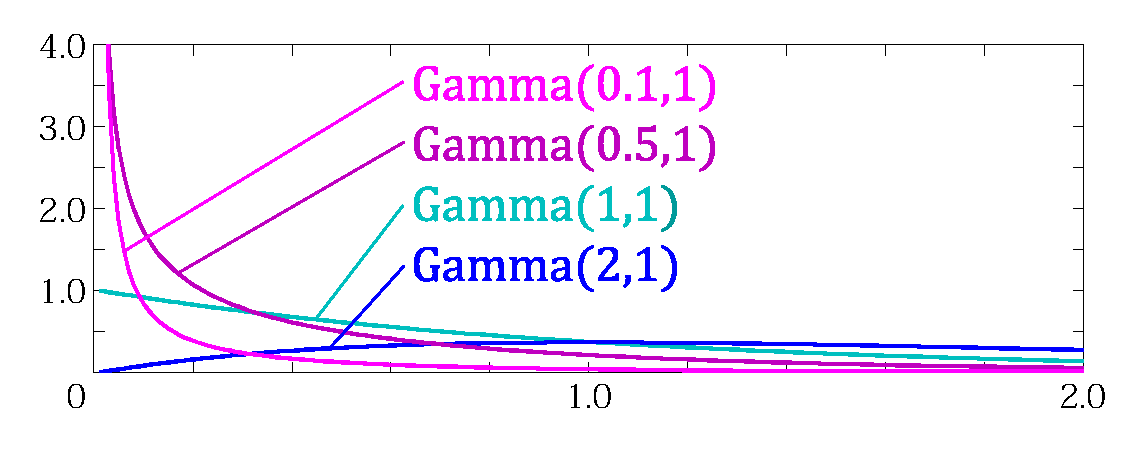
\includegraphics[width=.9\linewidth]{sections/factorization/gamma}
\caption{形状母数が異なる幾つかのガンマ分布.}
\label{fig:gamma}
\end{figure}

ガンマ過程に基づくNMFのノンパラメトリックベイズモデル (GaP-NMF)について説明する.
まず,\refeq{eqn:x_wh_elem}に対し,
$K$次元の非負値ベクトル
$\bm\theta = [\theta_1,\theta_2,\cdots,\theta_K]$を導入する.
\begin{align}
 \bm{x}_n \approx 
 \sum_{k=1}^{K} \theta_k h_{kn} \bm{w}_k \overset{\mbox{\tiny def}}{=} \bm{y}_n
\end{align}
ここで,$\theta_k \ge 0$は基底$k$の大域的な重みである.
この$\bm\theta$に対し,
観測データ$\bm{X}$を表現するのに必要な基底$k$以外の要素$\theta_k$が
ゼロとなるようなスパースな学習を行いたい.

ノンパラメトリックベイズモデルを定式化するため,
$\bm\theta$,$\bm{W}$,$\bm{H}$に対して事前分布を導入する.
まず,$\bm{W}$及び$\bm{H}$の各要素は非負値であるので,
ガンマ事前分布を用いると都合が良い.
\begin{align}
w_{km} &\sim \mbox{Gamma}(a_0^w, b_0^w)
\label{eqn:p_w_km}
\\
h_{kn} &\sim \mbox{Gamma}(a_0^h, b_0^h)
\label{eqn:p_h_kn}
\end{align}
ここで,$a_0^* > 0$及び$b_0^* > 0$はそれぞれ,
ガンマ分布の形状母数と逆尺度母数である.
更に,$\bm\theta$に対しても同様にガンマ事前分布を仮定する.
\begin{eqnarray}
 \theta_k \sim \mbox{Gamma}\left(\frac{\alpha c}{K}, \alpha\right)
  \label{eqn:p_t_k}
\end{eqnarray}
ここで,$\alpha > 0$及び$c > 0$は超パラメータである.
ガンマ分布の形状母数が小さくなるほど0が出る確率が大きくなる(\figref{fig:gamma}).
ただし,$\mathbb{E}_{\mbox{\scriptsize prior}}[\theta_k] = \frac{c}{K}$,
$\mathbb{E}_{\mbox{\scriptsize prior}}[\sum_k \theta_k] = c$である.

ここで,\refeq{eqn:p_w_km},\refeq{eqn:p_h_kn}及び\refeq{eqn:p_t_k}で構成される
有限モデルに対して,$K \rightarrow \infty$となる極限を考えると,
以下のガンマ過程が得られる.
\begin{eqnarray}
G \sim \mbox{GaP}(\alpha, G_0)
\end{eqnarray}
ここで,$G_0$は空間$U$($\bm{w} \in \mathbb{R}_+^M$と$\bm{h} \in \mathbb{R}_+^N$の直積空間)上に
定義された基底測度であり,$G_0(U) = c$を満たす(\figref{fig:gap}).
このとき,$G$は$U$上の離散測度となり,
空間$U$の任意の分割$\{U_i\}_{i=1}^I$に対して
\begin{align}
G(U_i) \sim \mbox{Gamma}(\alpha G_0(U_i), \alpha)
\end{align}
が成立している.ただし,$\mathbb{E}[G] = G_0$である.
微小区間への分割を$\{U_k\}_{k=1}^\infty$とすると,
$G(U_k) = \theta_k$である.
$\alpha$は集中度と呼ばれ,$\alpha$が小さくなるほど$\bm\theta$は
よりスパースになる.
計算機上では$K \rightarrow \infty$は扱えないが,
$K$を$\alpha$に比べて十分大きな値に設定すれば,
\refeq{eqn:p_t_k}はガンマ過程の良い近似となる(weak-limit approximation).
%この他,棒折り過程など他の構成法も利用可能と考えられる.

\begin{algorithm}[t]
\caption{GaP-KL-NMFのベイズ推定}
\label{kl-nmf-vb}
\begin{algorithmic}[1]
\Require 非負値行列$\bm{X} \in \mathbb{R}_+^{M \times N}$, 
最大基底数$K$,ガンマ過程の集中度$\alpha$,
ガンマ分布のパラメータ$a_0^w,b_0^w,a_0^h,b_0^h$
\State 変分事後分布$q(\bm\theta)$, $q(\bm{W})$, $q(\bm{H})$をランダムに初期化
\While{not converged}
\State $\lambda_{knm} \propto \mathbb{E}_{q}[\theta_k w_{km} h_{kn}]$
\State $\textstyle q(\theta_k)
= \mbox{Gamma}(\frac{\alpha c}{K} + \sum_{nm} \lambda_{knm} x_{nm},$\\
\ \ \ \ \ \ \ \ \ \ \ \ \ \ \ \ \ \ \ \ \ \ \ \ \ \ \ $\alpha + \sum_{nm} \mathbb{E}_{q}[w_{km} h_{kn}])$
\State $\textstyle q(w_{km}) 
= \mbox{Gamma}(a_0^w + \sum_{n} \lambda_{knm} x_{nm},$\\
\ \ \ \ \ \ \ \ \ \ \ \ \ \ \ \ \ \ \ \ \ \ \ \ \ \ \ \ \ \ $b_0^w + \sum_{n} \mathbb{E}_{q}[\theta_k h_{kn}])$
\State $\textstyle q(h_{kn}) 
= \mbox{Gamma}(a_0^h + \sum_{m} \lambda_{knm} x_{nm},$\\
\ \ \ \ \ \ \ \ \ \ \ \ \ \ \ \ \ \ \ \ \ \ \ \ \ \ \ \ \ $b_0^h + \sum_{m} \mathbb{E}_{q}[\theta_k w_{km}])$
\EndWhile\\
{\bf Return} 変分事後分布$q(\bm\theta)$, $q(\bm{W})$, $q(\bm{H})$
\end{algorithmic}
\end{algorithm}

\subsection{GaP-KL-NMFのベイズ推定}
\label{sec:gap-kl-nmf}

まず,GaP-KL-NMFに対するVBを導出する.
\refeq{eqn:lb}で与えられる変分下限$\mathcal{L}(q)$の第一項は
\refeq{eqn:kl_s_p}で計算できる対数ポアソン尤度の期待値であるが,
依然として解析的に計算できない.
そのため,凹関数$f(x)=\log(x)$に対してJensenの不等式を用いると
更なる変分下限
\begin{align}
&
\mathbb{E}_{q}[\log p(\bm{X}|\bm\theta,\bm{W},\bm{H})]
\nonumber\\
&
\overset{c}{=} \mathbb{E}_{q}\!\!\left[\sum_{nm} \left(x_{nm} \log \sum_k y_{knm} - \sum_k y_{knm}\right)\right]
\nonumber\\
&
= \sum_{nm} x_{nm} \mathbb{E}_{q}\!\!\left[\log \sum_k \lambda_{knm} \frac{y_{knm}}{\lambda_{knm}}\right] 
&
\nonumber\\
& \ \ \ \
- \sum_{knm} \mathbb{E}_{q}\!\left[y_{knm}\right]
\nonumber\\
%\end{align}
%
%\begin{align}
&
\ge \sum_{nm} x_{nm} \sum_k \lambda_{knm} \mathbb{E}_{q}\!\!\left[\log \frac{y_{knm}}{\lambda_{knm}}\right] 
&
\nonumber\\
& \ \ \ \ 
- \sum_{knm} \mathbb{E}_{q}\!\left[y_{knm}\right]
\nonumber\\
&\overset{\mbox{\scriptsize def}}{=} 
\mathbb{E}_{q}[\log q(\bm{X}|\bm\theta,\bm{W},\bm{H})]
\label{eqn:lb2_kl}
\end{align}
を得る.ここで,$\lambda_{knm}$は$\sum_k \lambda_{knm} = 1$を満たす補助変数である.
等号成立条件(変分下限が最大となる条件)はラグランジュの未定乗数法を用いて求めることができ,
$\lambda_{knm} \propto \mathbb{E}_{q}[y_{knm}]$となる.

\begin{algorithm}[t]
\caption{GaP-IS-NMFのベイズ推定}
\label{is-nmf-vb}
\begin{algorithmic}[1]
\Require 非負値行列$\bm{X} \in \mathbb{R}_+^{M \times N}$, 最大基底数$K$,ガンマ過程の集中度$\alpha$,
ガンマ分布のパラメータ$a_0^w,b_0^w,a_0^h,b_0^h$
\State 変分事後分布$q(\bm\theta)$, $q(\bm{W})$, $q(\bm{H})$をランダムに初期化
\While{not converged}
\State $\lambda_{knm} \propto \mathbb{E}_{q}[\theta_k^{-1} w_{km}^{-1} h_{kn}^{-1}]^{-1}$
\State $\omega_{nm} \propto \sum_k \mathbb{E}_{q}[\theta_k w_{km} h_{kn}]$
\State $\textstyle q(\theta_k)
= \mbox{GIG}(\frac{\alpha c}{K}, 
\alpha + \sum_{nm} \omega_{nm}^{-1} \mathbb{E}_{q}\!\left[w_{km}\right] \mathbb{E}_{q}\!\left[h_{kn}\right],$\\
\ \ \ \ \ \ \ \ \ \ \ \ \ \ \ \ \ \ \ \ \ \ \ \ \ \ \ \ \
$\sum_{nm} x_{nm} \lambda_{knm}^2 \mathbb{E}_{q}\!\left[w_{mk}^{-1}\right] \mathbb{E}_{q}\!\left[h_{kn}^{-1}\right])$
\State $\textstyle q(w_{km})
= \mbox{GIG}(a_0^w, 
b_0^w + \sum_{n} \omega_{nm}^{-1} \mathbb{E}_{q}\!\left[\theta_k\right] \mathbb{E}_{q}\!\left[h_{kn}\right],$\\
\ \ \ \ \ \ \ \ \ \ \ \ \ \ \ \ \ \ \ \ \ \ \ \ \ \ \ 
$\sum_{n} x_{nm} \lambda_{knm}^2 \mathbb{E}_{q}\!\left[\theta_k^{-1}\right] \mathbb{E}_{q}\!\left[h_{kn}^{-1}\right])$
\State $\textstyle q(h_{kn})
= \mbox{GIG}(a_0^h, 
\sum_{m} \omega_{nm}^{-1} \mathbb{E}_{q}\!\left[\theta_k\right] \mathbb{E}_{q}\!\left[w_{km}\right],$\\
\ \ \ \ \ \ \ \ \ \ \ \ \ \ \ \ \ \ \ \ \ \ \ \
$\sum_{m} x_{nm} \lambda_{knm}^2 \mathbb{E}_{q}\!\left[\theta_k^{-1}\right] \mathbb{E}_{q}\!\left[w_{km}^{-1}\right]$)
\EndWhile\\
{\bf Return} 変分事後分布$q(\bm\theta)$, $q(\bm{W})$, $q(\bm{H})$
\end{algorithmic}
\end{algorithm}

最後に,各パラメータに対する変分事後分布を導出する.
実際には\refeq{eqn:lb}で与えられる元の変分下限$\mathcal{L}(q)$ではなく,
\refeq{eqn:lb2_kl}を用いて得られた更なる変分下限を最大化することになる.
その結果,\refeq{eqn:q_t}, (\ref{eqn:q_w}), (\ref{eqn:q_h})において,
$\log p(\bm{X},\bm\theta,\bm{W},\bm{H})$の代わりに
次式を用いることになる.
\begin{eqnarray}
\log q(\bm{X},\bm\theta,\bm{W},\bm{H}) 
= \log q(\bm{X}|\bm\theta,\bm{W},\bm{H})
\nonumber\\
+ \log p(\bm\theta) + \log p(\bm{W}) + \log p(\bm{H})
\end{eqnarray}
具体的には,最適な変分事後分布$q(\bm\theta)$は,$\bm\theta$に関連する項のみを取り出すと
以下の通り計算できる.
\begin{align}
\log q(\bm\theta) 
&\overset{c}{=}
\sum_{knm} x_{nm} \lambda_{knm} \log \theta_k
\nonumber\\
&
- \sum_{knm} \theta_k \mathbb{E}_{q}\!\left[w_{km}\right] \mathbb{E}_{q}\!\left[h_{kn}\right]
\nonumber\\
&
+ \sum_{k} \left( \left(\frac{\alpha c}{K} - 1\right) \log \theta_k - \alpha \theta_k \right)
\end{align}
従って,$\theta_k$の事後分布はガンマ分布となる.
同様に,最適な$q(\bm{W})$や$q(\bm{H})$もガンマ分布として求まる.
{\bf Algorithm \ref{kl-nmf-vb}}に更新則を示す.
反復ごとに,$\mathbb{E}[\theta_k]$が十分に小さい基底$k$を削除していけば,
実効的な基底数$K_+$が自動的に定まる.

\subsection{GaP-IS-NMFのベイズ推定}

次に,GaP-IS-NMFに対するVB\cite{hoffman:icml:2010}を導出する.
\refeq{eqn:lb}で与えられる変分下限$\mathcal{L}(q)$の第一項は
\refeq{eqn:is_p}で与えられる対数指数尤度の期待値であり,
やはり解析的に計算できない.
そこで,凹関数$f(x) = - \frac{1}{x}$に対してJensenの不等式を考える.
\begin{align}
- \frac{1}{\sum_{k=1}^K x_k} 
= - \frac{1}{\sum_{k=1}^K \lambda_k \frac{x_k}{\lambda_k}} \ge \sum_{k=1}^K \frac{\lambda_k^2}{x_k}
\end{align}
ここで,$\lambda_k$は$\sum_k \lambda_k = 1$を満たす補助変数であり,
等号成立条件は$\lambda_k \propto x_k$である.
更に,凸関数$g(x) = - \log(x)$に対する1次のテイラー展開($\omega$における接線)を考える.
\begin{align}
- \log (x) \ge - \log (\omega) - \frac{x}{\omega} + 1
\end{align}
ここで,$\omega$は補助変数であり,等号成立条件は$\omega = x$である.
これら二つの不等式を用いると
変分下限$\mathbb{E}_{q}[\log q(\bm{X}|\bm\theta,\bm{W},\bm{H})]$を得る.
\begin{align}
&
\mathbb{E}_{q}[\log p(\bm{X}|\bm\theta,\bm{W},\bm{H})]
\nonumber\\
&
\overset{c}{=} \mathbb{E}_{q}\!\!\left[\sum_{nm} 
\left(- x_{nm} \left(y_{nm}\right)^{-1} - \log \left(y_{nm}\right)\right)\right]
\nonumber\\
&
\ge - \sum_{nm} x_{nm} \mathbb{E}_{q}\!\!\left[\sum_k \frac{\lambda_{knm}^2}{y_{knm}}\right] 
\nonumber\\
&\ \ \
- \sum_{nm} \left(\log(\omega_{nm}) + \mathbb{E}_{q}\!\!\left[\frac{y_{nm}}{\omega_{nm}}\right] - 1\right)
\nonumber\\
&
\overset{\mbox{\scriptsize def}}{=} \mathbb{E}_{q}[\log q(\bm{X}|\bm\theta,\bm{W},\bm{H})]
\label{eqn:lb2_is}
\end{align}

各パラメータに対する変分事後分布は,\refsubsec{sec:gap-kl-nmf}と同様に求められる.
具体的には,最適な変分事後分布$q(\bm\theta)$は,$\bm\theta$に関連する項のみを取り出すと
\begin{align}
&
\log q(\bm\theta) 
\overset{c}{=} 
- \sum_{knm} x_{nm} \lambda_{knm}^2 \theta_k^{-1} \mathbb{E}_{q}\!\!\left[w_{km}^{-1}\right] \mathbb{E}_{q}\!\!\left[h_{kn}^{-1}\right] 
\nonumber\\
&\ \
- \sum_{knm} \omega_{nm}^{-1} \theta_k \mathbb{E}_{q}\!\left[w_{km}\right] \mathbb{E}_{q}\!\left[h_{kn}\right]
\nonumber\\
&\ \ \ \
+ \sum_{k} \left( \left(\frac{\alpha c}{K} - 1\right) \log \theta_k - \alpha \theta_k \right)
\end{align}
従って,$\theta_k$の事後分布はGeneralized Inverse Gaussian (GIG) 分布となることが分かる
(詳細は\cite{hoffman:icml:2010}参照).
{\bf Algorithm \ref{is-nmf-vb}}に更新則を示す.

\subsection{BP-KL-NMFのベイズ推定}


\section{半正定値テンソル分解}

このような無限次元の空間($K\rightarrow\infty$)におけるスパースな学習は,
ノンパラメトリックベイズモデルを用いて実現することができる\cite{hoffman:icml:2010}.
近年,NMFの数学的に自然な拡張である半正定値テンソル分解 
(Positive Semidefinite Tensor Factorization: PSDTF)\cite{yoshii:icml:2013,yoshii:ismir:2013}が提案され,
優れた音源分離結果を達成している.

本章では,NMFの自然な拡張である
半正定値テンソル分解\cite{yoshii:icml:2013,yoshii:ismir:2013}(PSDTF) について解説する.
PSDTFでは,各フレーム$n$の複素スペクトル$\tilde{\bm{x}}_n$の
自己共分散$\bm{X}_n \!=\! \tilde{\bm{x}}_n\tilde{\bm{x}}_n^H$,
すなわち{\bf 半正定値行列を少数の半正定値行列の和に分解}する(\figref{fig:comparison}).
一方,NMFでは,上記行列の対角成分(パワースペクトル)
$\bm{x}_n \!=\! \tilde{\bm{x}}_n \odot \tilde{\bm{x}}_n^*$,すなわち
{\bf 非負値ベクトルを少数の非負値ベクトルの和に分解}する.
行列の半正定値性はベクトルの非負値性の拡張概念であり,
非負値テンソル分解 (Nonnegative Tensor Factorization: NTF) と
PSDTFとは異なる.

音源分離においては,観測スペクトログラム$\tilde{\bm{X}}$から,
\refeq{eqn:s}を満たす音源スペクトログラム$\tilde{\bm{X}}_k$の位相を推定できる.
音源信号の周期と短時間フーリエ変換の窓長$M$が異なると,
音源信号の巡回定常性の仮定が成り立たないため,
周波数ビン間の相関を取り扱える利点は大きい.
マルチチャネル音源分離において,
%周波数ビン間の相関行列ではなく,
マイク間の相関行列を分解する際にも同様のモデルが提案されている\cite{sawada:ieee:2013}.

\subsection{コスト関数最小化としての定式化}
\label{sec:ps}

\begin{figure}[t]
\centering
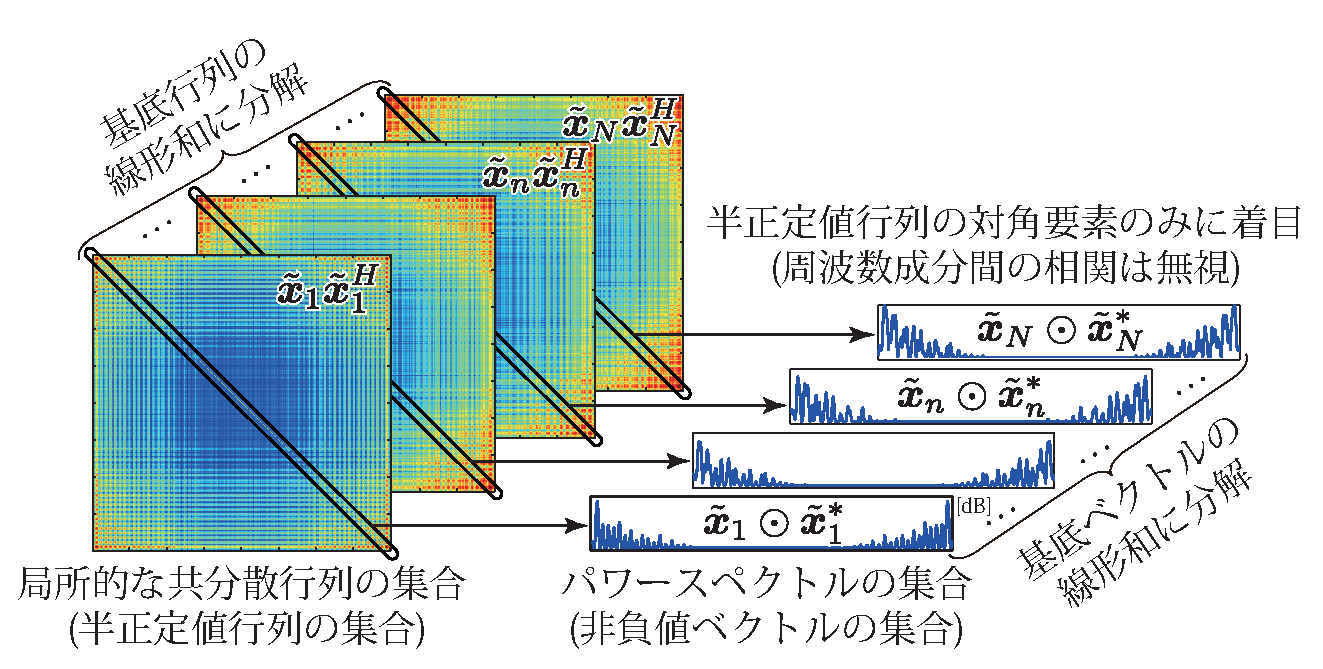
\includegraphics[width=\columnwidth]{sections/factorization/comparison}
\caption{音源分離のための半正定値テンソル分解 (PSDTF).}
\label{fig:comparison}
\end{figure} 

PSDTFでは,観測データとして3階のテンソル
$\bm{X} = [\bm{X}_1,\cdots,\bm{X}_n] \in \mathbb{C}^{M \times M \times N}$
に対する分解を行う.
各要素$\bm{X}_n \succeq \bm{0} \in \mathbb{C}^{M \times M}$は半正定値行列とする.
今,各$\bm{X}_n$を
$K$個の半正定値行列$\{\bm{W}_k\}_{k=1}^{K}$(基底行列)
の凸結合で近似したい.
\begin{align}
 \bm{X}_{n} \approx 
  \sum_{k=1}^{K} h_{kn} \bm{W}_k
  \overset{\mbox{\tiny def}}{=} \bm{Y}_n
 \label{eqn:x_n_psdtf}
\end{align}
ここで,$h_{kn} \ge 0$は$\bm{X}_n$における
基底行列$\bm{W}_k$の重みである.
観測行列$\bm{X}_n$と再構成行列$\bm{Y}_n$との間の誤差$\mathcal{D}(\bm{X}_n|\bm{Y}_n)$を
評価する尺度として,非負値ベクトル間のKLダイバージェンスや
ISダイバージェンスの拡張である,
半正定値行列間のvon-Neumann (vN) ダイバージェンスや
Log-Determinant (LD) ダイバージェンスがある\cite{kulis:jmlr:2009}.
\begin{align}
 &
 \mathcal{D}_{\mbox{\tiny vN}}(\bm{X}_n|\bm{Y}_n)
 = \mbox{tr}\left(\bm{X}_n \log \bm{X}_n - \bm{X}_n \log \bm{Y}_n\right.
 \nonumber\\
 & \ \ \ \ \ \ \ \ \ \ \ \ \ \ \ \ \ \ \ \ \ \
 \left.- \bm{X}_n + \bm{Y}_n\right)
 \label{eqn:psdtf_vn}\\
 &
 \mathcal{D}_{\mbox{\tiny LD}}(\bm{X}_n|\bm{Y}_n)
 = \mbox{tr}\left(\bm{X}_n \bm{Y}_n^{-1}\right)
 \nonumber\\
 & \ \ \ \ \ \ \ \ \ \ \ \ \ \ \ \ \ \ \ \ \ \
 - \log\left|\bm{X}_n \bm{Y}_n^{-1}\right|
 - M
 \label{eqn:psdtf_ld}
\end{align}

\subsection{乗法更新アルゴリズムに基づく最適化}
\label{sec:psdtf_mu}

コスト関数$\mathcal{D}(\bm{X}|\bm{Y})
 =\sum_n \mathcal{D}(\bm{X}_n|\bm{Y}_n)$
を最小化する
$\bm{H} = [\bm{h}_1,\cdots,\bm{h}_K] \in \mathbb{R}^{N \times K}$
及び$\bm{W} = [\bm{W}_1,\cdots,\bm{W}_K] \in \mathbb{C}^{M \times M \times K}$
を求めるため,LD-PSDTFに対しても%補助関数法に基づく収束性が保証された
乗法更新アルゴリズム\cite{yoshii:ismir:2013,yoshii:icml:2013}が提案されている.
更新則は{\bf Algorithm?\ref{ld-psdtf-ml}}で与えられる
(導出は文献\cite{yoshii:ismir:2013,yoshii:icml:2013}参照).
$h_{kn}$の非負性と
$\bm{W}_k$の半正定値性は自然に保たれているが,
$\mbox{tr}(\bm{W}_k)=1$を満たすよう,反復ごとに
$\bm{W}_k$及び$\bm{h}_k$をスケーリングしておく.
%{\bf Algorithm?\ref{ld-psdtf-ml}}は,
%{\bf Algorithm?\ref{is-nmf-ml}}の自然な拡張である.

\section{確率的潜在成分解析}

Probabilitic Latent Component Analysis

\subsection{確率モデルの最尤推定としての定式化}

\subsection{ノンパラメトリックベイズモデル}

\subsection{音源分離への応用}



\chapter{音声信号処理}

\begin{leadbox}
音声.
\end{leadbox}

\section{音声分析合成}
\label{sec:lpc_intro}

我々人間は,喉頭と声帯を用いた発声と声道による調音をおおよそ独立に制御しながら声を発します。
音声分析合成とは,音声生成過程を模擬したモデルを用いて
音声信号の各短時間区間における声帯の音源特性と声道の共振特性を推定し,
音声認識,音声合成,音声変換,音声符号化
などに役立てるための技術です。
音声信号のみから声帯音源特性と声道共振特性を推定する問題は,
$XY=10$という式から$X$と$Y$を推定する問題と似ていて,
何らかの仮定を置かない限り解が一意に定まりません。
従って,声帯音源や声道に関してどのような仮定を置くかが問題解決のポイントになります。
これらの仮定の置き方に応じてこれまで多くの手法が提案されていますが,
中でも特に有名かつ基礎的なのが線形予測分析と呼ぶ手法で,
音声音響信号処理の分野に多大な影響を与え,
統計的手法による音声情報処理の枠組を生むきっかけの一つになった重要技術です.
また,現在も携帯電話やVoIPの音声符号化圧縮方式の基礎技術として用いられています.
そこで,\ref{sec:LPC}ではまず線形予測分析の理論を解説します。


\subsection{線形予測分析}
\label{sec:LPC}

以下,線形予測分析の目的とそれを実現するための最適化問題,
確率モデルの最尤パラメータ推定問題としての解釈,
パラメータ推定のためのアルゴリズム,音声の生成過程との関係性,周波数領域での解釈,などについて述べていきます。
読み進めていくうちにいかに奥深くエレガントな理論であるかを分かっていただけるのではないかと思います。

\subsubsection{問題の定式化}
\label{subsec:TD_LPC}

線形予測分析の目的自体は大変シンプルで,
信号の現時刻の標本値を過去の標本値の線形結合でできるだけ良く近似できるように結合係数を決めることです.
これが「線形予測」分析と呼ばれる所以です.
音声信号のように近い時刻間で強い相関があるような信号の場合,
その相関を活かすことで信号を少ないパラメータで表現できるだろうという考え方がベースになっています.
%線形予測分析はこの考え方が基礎になっていて,
%このような動機から信号の符号化圧縮に応用されています.
線形予測分析が
なぜ音声の声帯の音源特性と声道の共振特性を推定する手法になっているのか
についてはおいおい説明していくことにして,ここではまず
以上の問題を具体的に定式化していくことにします.

音声信号は大域的に見れば非定常ですが,短い区間に区切ればそれぞれの区間では近似的に定常と見なせます.
そこで,ある短区間の音声信号の標本値を$x_1,x_2,\ldots,x_N$とし,この系列に対し定常性を仮定します.
線形予測分析は,時刻$t_n$の信号の標本値$x_n$を
時刻$t_n$より過去の標本値$x_{n-1},x_{n-2},\ldots,x_{n-P}$
の線形結合で予測できるようにすることが目的で,
\begin{align}
\mathcal{J}(\Vec{a}) =
\sum_n \left(
x_n - \sum_{p=1}^{P} a_p x_{n-p}
\right)^2
\label{eq:lp}
\end{align}
を最小化する結合係数$\Vec{a} = (a_1,\ldots,a_P)^{\mathsf T}$
を求める最適化問題として定式化されます.
この結合係数を「予測係数」と呼びます.
この最適化問題は,
$\Vec{x} =(x_1,\ldots,x_N)^{\mathsf T}$を
%$P$次の
自己回帰過程
\begin{align}
x_n &= 
\sum_{p=1}^P a_p x_{n-p} + y_n
\label{eq:AR}\\
y_n  &\mathop{\sim}^{iid} \mathcal{N}(y_n;0,\sigma^2)~~
\label{eq:Gaussnoise}
\end{align}
から生成された観測値系列
と仮定した場合の$\Vec{a} = (a_1,\ldots,a_P)^{\mathsf T}$
の最尤推定問題
と等価になります\cite{Itakura1972}.このことを以下で確認しましょう.
ただし,$\mathcal{N}$は正規分布の確率密度関数
\begin{align}
\mathcal{N}(\Vec{x};\Vec{\mu},\Vec{\Sigma})= \frac{1}{(2\pi)^{N/2}|\det(\Vec{\Sigma})|^{1/2}}
e^{-\frac{1}{2}(\Vec{x}-\Vec{\mu})^{\mathsf T}\Vec{\Sigma}^{-1}(\Vec{x}-\Vec{\mu})}
\end{align}
を表すものとします.
\refeq{Gaussnoise}は$y_n$が独立に同一(平均0,分散$\sigma^2$)の
正規分布に従うことを意味します.
%つまり$\{y_n\}$は定常白色Gauss過程です.
$y_n$は
$\sum_{p=1}^P a_p x_{n-p}$による$x_n$の
予測の誤差を表す確率変数なので,「予測誤差」と呼びます.
$\Vec{y} = (y_1,\ldots,y_T)^{\mathsf T}$
とし,
\begin{align}
\Vec{\Psi} = 
\begin{bmatrix}
\hspace{-0ex}1& & & & &\hspace{-1.7ex}0\vspace{-1.7ex}\\
\hspace{-0ex}-a_1&\hspace{-1.7ex}\ddots& & & &\vspace{-1.7ex}\\
\hspace{-0ex}\vdots&\hspace{-1.7ex}\ddots&\hspace{-1.7ex}\ddots& & &\vspace{-1.7ex}\\
\hspace{-0ex}-a_P& &\hspace{-1.7ex}\ddots &\hspace{-1.7ex}\ddots& &\vspace{-1.7ex}\\
 &\hspace{-1.7ex}\ddots& &\hspace{-1.7ex}\ddots&\hspace{-1.7ex}\ddots&\vspace{-1.7ex}\\
\hspace{-0ex}0 & &\hspace{-1.7ex}-a_P&\hspace{-1.7ex}\cdots&\hspace{-1.7ex}-a_1&\hspace{-1.7ex}1
\end{bmatrix}
\label{eq:Psi}
\end{align}
と置くと,\refeq{AR}は
\begin{align}
\Vec{\Psi}\Vec{x} =\Vec{y}
\label{eq:AR2}
\end{align}
のように書けます.$\Vec{\Psi}$は対角成分がすべて1の下三角行列なので$\det(\Vec{\Psi})=1$が言え,
逆行列をもちます.従って,
$\Vec{y}\sim \mathcal{N}(\Vec{y};\Vec{0},\sigma^2\Vec{I})$および
\refeq{AR2}
より,$\Vec{x}$は平均が0,分散共分散行列が$\sigma^2 \Vec{\Psi}^{-1}\Vec{\Psi}^{-\mathsf T}$の正規分布に従います.
\begin{align}
\Vec{x} \sim \mathcal{N}(\Vec{x};\Vec{0},\sigma^2 \Vec{\Psi}^{-1}\Vec{\Psi}^{-\mathsf T})
\label{eq:s_pdf}
\end{align}
$\det(\Vec{\Psi})=1$より,
$\Vec{x} =(x_1,\ldots,x_N)^{\mathsf T}$が観測された下での
$\Vec{a}$の対数尤度は
\begin{align}
\log p(\Vec{x}|\Vec{a}) 
=
%-\frac{T}{2}\log(2\pi\sigma^2)- \frac{1}{2\sigma^2}\Vec{s}^{\mathsf T}\Vec{\Psi}^{\mathsf T}\Vec{\Psi}\Vec{s}
%\nonumber\\
%=&
-\frac{N}{2}\log(2\pi\sigma^2)
- 
\frac{1}{2\sigma^2}
\sum_n 
\left(x_n - \sum_{p=1}^{P} a_p x_{n-p}\right)^2
\label{eq:lpc_loglikelihood}
\end{align}
となるので,$\Vec{a}$によらない項を除けば
\refeq{lp}の正負を逆転したものと等しくなります.
以上よりたしかに\refeq{lp}を$\Vec{a}$に関して最小化することと
\refeq{lpc_loglikelihood}を$\Vec{a}$に関して最大化することは
等価であることが分かります.

$\mathcal{J}(\Vec{a})$を$a_q$に関して偏微分して
0と置き,
\begin{align}
\frac{\partial\mathcal{J}(\Vec{a})}{\partial a_q}
&=
%2
%\sum_n
%\left(
%x_n-\sum_{p=1}^{P}
%a_p x_{n-p}
%\right)
%(-x_{n-q})
%\nonumber\\
%&=
2
\bigg(
\sum_p a_p
\sum_n x_{n-p}x_{n-q}
-
\sum_n x_n x_{n-q}
\bigg)
=0
\end{align}
を$q = 1,\ldots, P$について連立させると,
\begin{align}
\begin{bmatrix}
r_{1,1} & r_{1,2} & \cdots & r_{1,P}\\
r_{2,1} & r_{2,2} & \cdots & r_{2,P}\\
\vdots  & \vdots & & \vdots\\
r_{P,1} & r_{P,2} & \cdots & r_{P,P}
\end{bmatrix}
\begin{bmatrix}
a_1\\
a_2\\
\vdots\\
a_P
\end{bmatrix}
=
\begin{bmatrix}
r_{0,1}\\
r_{0,2}\\
\vdots\\
r_{0,P}
\end{bmatrix}
\label{eq:lpc_YuleWalker}\\
r_{q,p} = \sum_{n} x_{n-p}x_{n-q}
\end{align}
という形を得ます.よって
$\mathcal{J}(\Vec{a})$を最小化する$\Vec{a}$は
上式を解くことで得られます.
ここで,$\{x_n\}$がエルゴード的である(集合平均と時間平均が等しい)ならば
$r_{q,p}$は$x_n$の自己相関関数$\mathbb{E}[x_{n-p}x_{n-q}]$となり,
さらに$x_n$が弱定常である(自己相関が時間差のみに依存する)ならば,
$r_{q,p} = v_{|p-q|}$と置くことができます.このとき,
\refeq{lpc_YuleWalker}は
\begin{align}
\begin{bmatrix}
v_{0} & v_{1} & \cdots & v_{P-1}\\
v_{1} & v_{0} & \ddots & \vdots\\
\vdots & \ddots & \ddots & v_{1}\\
v_{P-1} & \cdots & v_{1} & v_{0}
\end{bmatrix}
\begin{bmatrix}
a_1\\
a_2\\
\vdots\\
a_P
\end{bmatrix}
=
\begin{bmatrix}
v_{1}\\
v_{2}\\
\vdots\\
v_{P}
\end{bmatrix}
\label{eq:lpc_YuleWalker2}
\end{align}
と書けます.この特殊な形の連立一次方程式をYule-Walker方程式といい,
次章の方法により解を効率的に計算することができます.



\subsection{Levinson-Durbinアルゴリズム}

ここでは,\refeq{lpc_YuleWalker2}のYule-Walker方程式の解を計算するための
効率的なアルゴリズムについて述べます.
一般的な連立一次方程式の解法としてはGaussの消去法が知られていますが,
\refeq{lpc_YuleWalker2}をGaussの消去法を用いて解く場合,計算オーダーは$\mathcal{O}(P^3)$になります.
係数行列が実対称行列であることを活かせばCholesky分解を用いた方法,
係数行列がToeplitz行列であることを活かせばLevinson-Durbinアルゴリズムと呼ぶ方法
を使うことができます.
この場合の計算オーダーはいずれも$\mathcal{O}(P^2)$となります.
一方,今解きたい方程式は,係数行列がToeplitz型であるとともに実対称
でもある特殊なクラスに属しています.
このようなクラスの連立一次方程式の解は,
Levinson-Durbinアルゴリズムで
$\mathcal{O}(P\log P)$の計算オーダーで計算することができます.

\refeq{lpc_YuleWalker2}を満たす$\Vec{a}$を
$\hat{\Vec{a}}^{(P)} = (\hat{a}_1^{(P)},\ldots,\hat{a}_P^{(P)})^{\mathsf T}$とし,
これを$P$次の最適な予測係数と呼ぶことにします.
Levinson-Durbinアルゴリズムでは,$m$次の最適な予測係数$\hat{\Vec{a}}^{(m)}$と
$m+1$次の最適な予測係数$\hat{\Vec{a}}^{(m+1)}$の間の関係式を用いて$\hat{\Vec{a}}^{(1)}$から$\hat{\Vec{a}}^{(P)}$を再帰的に解いていくことが基本方針となります.

まず,$m$次の最適な予測係数$\hat{\Vec{a}}^{(m)}$が満たすべきYule-Walker方程式
(\refeq{lpc_YuleWalker2}において$P = m$としたもの)を考えます.
\refeq{lpc_YuleWalker2}において右辺を左辺に移項し,
\begin{align}
\sigma_m^2 = v_0 - \sum_{p=1}^{m} \hat{a}_p^{(m)} v_p 
\label{eq:sigma_P}
\end{align}
と置けば,\refeq{lpc_YuleWalker2}を
\begin{align}
\begin{bmatrix}
v_{0}&v_{1}&\cdots&v_{m}\\
v_1&v_0&\cdots&v_{m-1}\\
\vdots&\vdots&\ddots&\vdots\\
v_{m}&v_{m-1}&\cdots&v_{0}
\end{bmatrix}
\begin{bmatrix}
1\\
-\hat{a}_1^{(m)}\\
\vdots\\
-\hat{a}_q^{(m)}
\end{bmatrix}
=
\begin{bmatrix}
\sigma_m^2\\
0\\
\vdots\\
0
\end{bmatrix}
\label{eq:LevinsonDurbin_1}
\end{align}
と書き換えることができます.
同様に,$m+1$次の最適な予測係数は
\begin{align}
\begin{bmatrix}
v_{0}&v_{1}&\cdots&v_{m+1}\\
v_1&v_0&\cdots&v_{m}\\
\vdots&\vdots&\ddots&\vdots\\
v_{m+1}&v_{m}&\cdots&v_{0}
\end{bmatrix}
\begin{bmatrix}
1\\
-\hat{a}_1^{(m+1)}\\
\vdots\\
-\hat{a}_{m+1}^{(m+1)}
\end{bmatrix}
=
\begin{bmatrix}
\sigma_{m+1}^2\\
0\\
\vdots\\
0
\end{bmatrix}
\label{eq:LevinsonDurbin_2}
\end{align}
を満たします.
ここで,係数行列の構造を活かしながら,
\refeq{LevinsonDurbin_1}を
\refeq{LevinsonDurbin_2}と同じ形とサイズになるように等価変形し,
$\hat{\Vec{a}}^{(m)} = (\hat{a}_1^{(m)},\ldots,\hat{a}_m^{(m)})^{\mathsf T}$
と$\hat{\Vec{a}}^{(m+1)} = (\hat{a}_1^{(m+1)},\ldots,\hat{a}_{m+1}^{(m+1)})^{\mathsf T}$
の関係を導きます.
まず,
\refeq{LevinsonDurbin_1}の左辺の行列の$m+2$列目に$(v_{m+1},v_{m},\ldots,v_1)^{\mathsf T}$
という列を追加し,この列による影響をなくすため
ベクトル$(1,-\hat{a}_1^{(m)},\ldots,-\hat{a}_m^{(m)})^{\mathsf T}$の第$m+2$要素に0を追加する
ことで,
\begin{align}
\left[
\begin{array}{cccc:c}
v_{0}&v_{1}&\cdots&v_{q}&v_{m+1}\\
v_1&v_0&\cdots&v_{m-1}&v_{m}\\
\vdots&\vdots&\ddots&\vdots&\vdots\\
v_{m}&v_{m-1}&\cdots&v_{0}&v_{1}
\end{array}
\right]
%\begin{bmatrix}
%v_{0}&v_{1}&\cdots&v_{P}&v_{P+1}\\
%v_1&v_0&\cdots&v_{P-1}&v_{P}\\
%\vdots&\vdots&\ddots&\vdots&\vdots\\
%v_{P}&v_{P-1}&\cdots&v_{0}&v_{1}
%\end{bmatrix}
\left[
\begin{array}{c}
1\\
-\hat{a}_1^{(m)}\\
\vdots\\
-\hat{a}_m^{(m)}\\
\hdashline
%\rowcolor[gray]{.8}
0
\end{array}
\right]
%\begin{bmatrix}
%1\\
%-\hat{a}_1^{(P)}\\
%\vdots\\
%-\hat{a}_P^{(P)}\\
%0
%\end{bmatrix}
=
\begin{bmatrix}
\sigma_m^2\\
0\\
\vdots\\
0
\end{bmatrix}
\label{eq:LevinsonDurbin_3}
\end{align}
と書き換えることができます.
次に,
\refeq{LevinsonDurbin_1}の左辺の行列の$m+2$行目に$(v_{m+1},v_{m},\ldots,v_1,v_0)$という行を追加し,
右辺のベクトルの第$m+2$要素に
\begin{align}
w_m = v_{m+1} - \sum_{p=1}^{m} \hat{a}_p^{(m)} v_{m-p+1}
\label{eq:w_P}
\end{align}
を追加することで,
\begin{align}
\left[
\begin{array}{ccccc}
v_{0}&v_{1}&\cdots&v_{m}&v_{m+1}\\
v_1&v_0&\cdots&v_{m-1}&v_{m}\\
\vdots&\vdots&\ddots&\vdots&\vdots\\
v_{m}&v_{m-1}&\cdots&v_{0}&v_{1}\\
\hdashline
v_{m+1}&v_{m}&\cdots&v_{1}&v_{0}
\end{array}
\right]
%\begin{bmatrix}
%v_{0}&v_{1}&\cdots&v_{P}&v_{P+1}\\
%v_1&v_0&\cdots&v_{P-1}&v_{P}\\
%\vdots&\vdots&\ddots&\vdots\\
%v_{P}&v_{P-1}&\cdots&v_{0}&v_{1}\\
%v_{P+1}&v_{P}&\cdots&v_{1}&v_{0}
%\end{bmatrix}
\begin{bmatrix}
1\\
-\hat{a}_1^{(m)}\\
\vdots\\
-\hat{a}_m^{(m)}\\
0
\end{bmatrix}
=
\left[
\begin{array}{c}
\sigma_m^2\\
0\\
\vdots\\
0\\
\hdashline
w_{m}
\end{array}
\right]
%\begin{bmatrix}
%\sigma_P^2\\
%0\\
%\vdots\\
%0\\
%w_{P}
%\end{bmatrix}
\label{eq:LevinsonDurbin_4}
\end{align}
と書くことができます.
これで\refeq{LevinsonDurbin_4}の左辺の行列を\refeq{LevinsonDurbin_2}の左辺の行列と同じ形とサイズにすることができました.
ここで,左辺の行列が対称かつToeplitz型になっているので,\refeq{LevinsonDurbin_4}において
左辺と右辺のベクトルの要素の順序を反転させたもの
\begin{align}
\begin{bmatrix}
v_{0}&v_{1}&\cdots&v_{m}&v_{m+1}\\
v_1&v_0&\cdots&v_{m-1}&v_{m}\\
\vdots&\vdots&\ddots&\vdots&\vdots\\
v_{m}&v_{m-1}&\cdots&v_{0}&v_{1}\\
v_{m+1}&v_{m}&\cdots&v_{1}&v_{0}
\end{bmatrix}
\begin{bmatrix}
0\\
-\hat{a}_m^{(m)}\\
\vdots\\
-\hat{a}_1^{(m)}\\
1
\end{bmatrix}
=
\begin{bmatrix}
w_{m}\\
0\\
\vdots\\
0\\
\sigma_m^2
\end{bmatrix}
\label{eq:LevinsonDurbin_5}
\end{align}
も同様に成り立ちます.
\refeq{LevinsonDurbin_4}と
\refeq{LevinsonDurbin_5}の左辺の行列は等しいので,
\refeq{LevinsonDurbin_4}から\refeq{LevinsonDurbin_5}に任意の値$K_m$を乗じたものを引くことで,
\begin{align}
\begin{bmatrix}
v_{0}&v_{1}&\cdots&v_{m}&v_{m+1}\\
v_1&v_0&\cdots&v_{m-1}&v_{m}\\
\vdots&\vdots&\ddots&\vdots&\vdots\\
v_{m}&v_{m-1}&\cdots&v_{0}&v_{1}\\
v_{m+1}&v_{m}&\cdots&v_{1}&v_{0}
\end{bmatrix}
\begin{bmatrix}
1-0\\
-\hat{a}_1^{(m)}+K_m \hat{a}_m^{(m)}\\
\vdots\\
-\hat{a}_m^{(m)}+K_m \hat{a}_1^{(m)}\\
0-K_m
\end{bmatrix}
=
\begin{bmatrix}
\sigma_m^2-K_m
w_{m}\\
0\\
\vdots\\
0\\
w_{m}-K_m\sigma_m^2
\end{bmatrix}
\label{eq:LevinsonDurbin_6}
\end{align}
という形を得ます.
さてここで,\refeq{LevinsonDurbin_6}と
\refeq{LevinsonDurbin_2}を比較してみましょう.
$K_m$は任意に選んで良いので,
\refeq{LevinsonDurbin_6}の右辺の第$m+2$要素が
\refeq{LevinsonDurbin_2}と同様に0になるように
\begin{align}
K_m = \frac{w_m}{\sigma_m^2}
\label{eq:PARCOR}
\end{align}
と選べば,
\refeq{LevinsonDurbin_6}を
\refeq{LevinsonDurbin_2}と同じ形にすることができます.
よって,そのときの
二式を比較することで,
\begin{align}
\begin{split}
\sigma_{m+1}^2 &= \sigma_m^2 - K_m w_m\\
\hat{a}_p^{(m+1)} &= \hat{a}_p^{(m)} - K_m \hat{a}_{m-p+1}^{(m)}~~(p=1,\ldots,m)\\
\hat{a}_{m+1}^{(m+1)} &= K_m
\end{split}
\label{eq:LevinsonDurbinRecursion}
\end{align}
という関係式を得ることができます.
\refeq{LevinsonDurbinRecursion}は
$m$次の最適な予測係数から$m+1$次の最適な予測係数を導く再帰式となっているため,
Levinson-Durbin再帰式と言います.
$1$次の最適な予測係数$\hat{a}_1^{(1)}$は\refeq{lpc_YuleWalker2}より
\begin{align}
\hat{a}_1^{(1)} = \frac{v_1}{v_0}
\end{align}
と容易に求まり,\refeq{sigma_P}と\refeq{w_P}より$\sigma_1^2$と$w_1$はそれぞれ
\begin{align}
\sigma_1^2 &=
v_0 - \hat{a}_1^{(1)} v_1
\\
w_1 &= v_2 - \hat{a}_1^{(1)} v_1
\end{align}
となるので,これらを初期値として上述の再帰式を用いて
$\hat{\Vec{a}}^{(2)} = (\hat{a}_{1}^{(2)},\hat{a}_2^{(2)})^{\mathsf T}$, 
$\hat{\Vec{a}}^{(3)} = (\hat{a}_{1}^{(3)},\hat{a}_2^{(3)},\hat{a}_{3}^{(3)})^{\mathsf T},
\ldots,~\hat{\Vec{a}}^{(P)} = (\hat{a}_{1}^{(P)},\ldots,\hat{a}_{P}^{(P)})^{\mathsf T}$
を再帰的に求めていくことができます.
以上がLevinson-Durbinアルゴリズムです.

ところで,Levinson-Durbin再帰式の導出の過程で導かれた
\refeq{PARCOR}の$K_m$は
偏自己相関係数(Partial Correlation Coefficients; PARCOR)と呼ばれていて,実は
物理的に重要な意味をもちます.
このことは\refsubsec{acoustic_cube_model}で詳しく述べることとします.

以上で求めた$P$次の最適な予測係数$\hat{\Vec{a}}$を$\Vec{\Psi}$に代入すれば,
\refeq{AR2}より$\Vec{x}$から
予測誤差系列$\Vec{y}$を得ることができます.
逆に,予測係数$\hat{\Vec{a}}$と予測誤差系列$\Vec{y}$のペア
から,
\begin{align}
x_1 = y_1,~~~
x_2 = y_2 + \hat{a}_1 x_1,~~~
x_3 = y_3 + \hat{a}_1 x_2 + \hat{a}_2 x_1,~~~
\ldots
\end{align}
のように$\Vec{x}$の要素を逐次的に復元することができます.


\subsection{声道スペクトル推定としての解釈}
\label{subsec:FD_LPC}

\begin{figure}[t!]
\centering
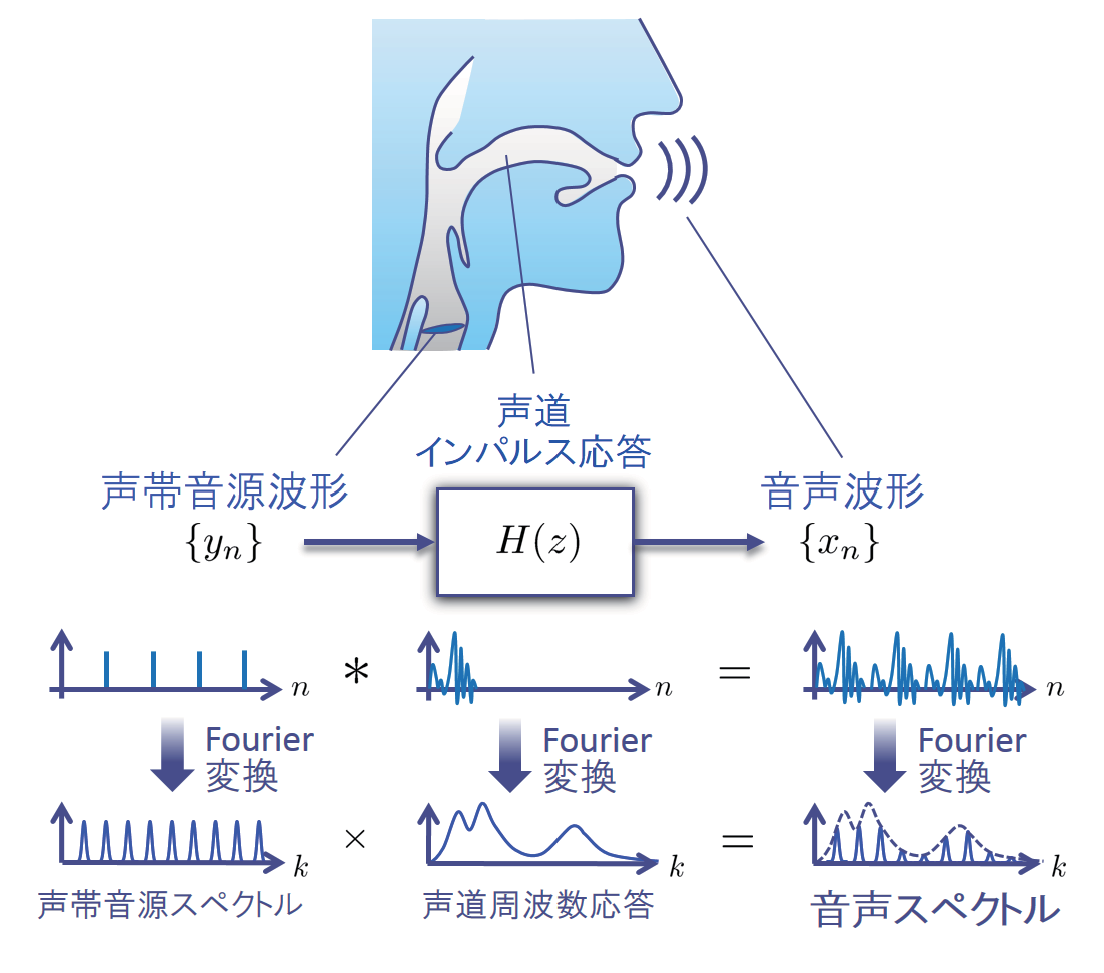
\includegraphics[width=.98\linewidth,keepaspectratio=true]{sections/speech/sourcefiltermodel3.eps}
\vspace{0ex}
 \caption{ソースフィルタ理論による音声生成過程モデル}
\label{fig:sourcefiltermodel}
\vspace{0ex}
\end{figure}

音声信号は,声帯によって発せられ声道による共振を受けた音波が,口唇から放射されたものです.
声道を線形フィルタと見なせば音声信号は声帯音源信号を入力した線形系の応答と見なせます(\reffig{sourcefiltermodel}).
このような音声信号の生成過程のモデル化は{\bf ソースフィルタ理論}と呼ばれています\cite{Chiba1941,Fant1960}.
予測誤差$\{y_n\}$を声帯音源信号,
予測係数$\Vec{a} = (a_1,\cdots,a_P)^{\mathsf T}$を
声道のフィルタ特性(声道スペクトル)を特徴付けるパラメータと見なせば,線形予測分析は
ソースフィルタ理論の解釈の下で
周波数領域において音声の声道スペクトル推定を行っていることに相当します.
以下ではこのことを示します.


音声信号$\{x_n\}$と予測誤差系列$\{y_n\}$の関係は
\begin{align}
y_n = x_n - \sum_{p=1}^{P} a_p x_{n-p}
\end{align}
で与えられます.$X(z)$と$Y(z)$をそれぞれ$\{x_n\}$と$\{y_n\}$の
$z$変換(?章参照)とすると,
\begin{align}
Y(z) &= A(z)X(z)\\
A(z) &= 1 - a_1 z^{-1} - a_2 z^{-2} \cdots - a_P z^{-P}
\end{align}
となるため,音声信号を入力として予測誤差系列を出力とする系は$A(z)$
を伝達関数とする線形時不変系で表されます.
逆に,予測誤差系列$\{y_n\}$を入力として音声信号$\{x_n\}$を出力とする
系の伝達関数は$A(z)$の逆数
\begin{align}
H(z) = \frac{1}{A(z)}
\end{align}
となります.この伝達関数は零をもたず極のみをもちますが,
?章で述べたとおり
このように極のみからなるシステムを全極システムといいます.
すなわち,もし音声信号の生成過程が線形時不変系で表せて,
予測誤差系列$\{y_n\}$を声帯音源信号と見なすことができれば,
声道の共振特性を全極型の伝達関数で表現していることになります.
$k=1,\ldots,N$を周波数インデックスとすると,
$z$変換において$z = e^{2\pi\j(k-1)/N}$としたものは離散Fourier変換
と一致します.従って,
$H(e^{2\pi\j(k-1)/N})$は全極システムの周波数応答となります.
また,$|H(e^{2\pi\j(k-1)/N})|^2$を全極スペクトルと呼びます.
実は声道フィルタとして全極システムを仮定することは
声道を無損失系の等長音響管でモデル化していることに相当します.
このことは\refsubsec{acoustic_cube_model}で詳しく述べることにして,
ここでは線形予測分析が周波数領域で何を行っていることに相当するのか
を明らかにします.

\refsubsec{TD_LPC}では
線形予測分析は時間領域では\refeq{s_pdf}を尤度関数とした予測係数$\Vec{a}$
の最尤推定問題として定式化されることを示しました.ここでは,$\Vec{x}$
の離散Fourier変換の尤度関数を導きます.
$\Vec{F}$を各行に異なる周波数の
複素正弦波が格納された離散Fourier変換行列
\begin{align}
\Vec{F} 
%&= (e^{e^{2\pi\j k n /N}})_{k,n}\\ 
&=
\frac{1}{\sqrt{N}}
\begin{bmatrix}
1&1&1&\cdots&1\\
1&e^{2\pi\j1/N}&e^{2\pi\j2/N}&\cdots&e^{2\pi\j(N-1)/N}\\
\vdots&\vdots&\vdots& &\vdots\\
1&\!\!e^{2\pi\j(N-1)/N}\!\!&\!\!e^{2\pi\j(N-1)2/N}\!\!&\!\!\cdots\!\!&\!\!e^{2\pi\j(N-1)(N-1)/N}
\end{bmatrix}
\end{align}
とすると,
$\Vec{x}$の離散Fourier変換は${\Vec{\chi}} = \Vec{Fx}$
で与えられ,$\Vec{\chi}=(\chi_1,\ldots,\chi_N)^{\mathsf T}$
の第$k$要素は周波数$k$の成分を表します.
$\Vec{F}$はユニタリ行列で
$|\det(\Vec{F})|=1$なので,確率密度関数の変数変換により,$\Vec{\chi}$は
平均が$\Vec{0}$,
分散共分散行列が$\sigma^2 \Vec{F}\Vec{\Psi}^{-1}\Vec{\Psi}^{- \mathsf T}\Vec{F}^{\mathsf H}$
の複素正規分布に従います.
\begin{align}
\Vec{\chi} \sim \mathcal{N}_{\mathbb{C}}(\Vec{\chi};\Vec{0},\sigma^2 
\Vec{F}\Vec{\Psi}^{-1}\Vec{\Psi}^{- \mathsf T}\Vec{F}^{\mathsf H})
\label{eq:c_pdf}
\end{align}
ただし,$\mathcal{N}_{\mathbb{C}}(\Vec{x};\Vec{\mu},\Vec{\Sigma}) = \frac{1}{\pi^N |\det(\Vec{\Sigma})|}e^{-(\Vec{x}-\Vec{\mu})^{\mathsf H}\Vec{\Sigma}^{-1}(\Vec{x}-\Vec{\mu})}$です.
ここで,分析窓の両端点において信号が巡回していると仮定し,
\refeq{Psi}の代わりに$\Vec{\Psi}$を
\begin{align}
\Vec{\Psi} = 
\begin{bmatrix}
\hspace{-0ex}1& & &\hspace{-1.7ex}-a_P&\hspace{-1.7ex}\cdots&\hspace{-1.7ex}-a_1\vspace{-1.7ex}\\
\hspace{-0ex}-a_1&\hspace{-1.7ex}\ddots& & &\hspace{-1.7ex}\ddots&\hspace{-1.7ex}\vdots\vspace{-1.7ex}\\
\hspace{-0ex}\vdots&\hspace{-1.7ex}\ddots&\hspace{-1.7ex}\ddots& & &\hspace{-1.7ex}-a_P\vspace{-1.7ex}\\
\hspace{-0ex}-a_P& &\hspace{-1.7ex}\ddots &\hspace{-1.7ex}\ddots& &\vspace{-1.7ex}\\
 &\hspace{-1.7ex}\ddots& &\hspace{-1.7ex}\ddots&\hspace{-1.7ex}\ddots&\vspace{-1.7ex}\\
\hspace{-0ex}0 & &\hspace{-1.7ex}-a_P&\hspace{-1.7ex}\cdots&\hspace{-1.7ex}-a_1&\hspace{-1.7ex}1
\end{bmatrix}
\label{eq:Psi2}
\end{align}
のような巡回行列とします.巡回行列同士の積は巡回行列になり,また,
巡回行列は離散Fourier変換行列により対角化されるため,
\begin{align}
\sigma^2
\Vec{F}\Vec{\Psi}^{-1}\Vec{\Psi}^{- \mathsf T}\Vec{F}^{\mathsf H}
&=\sigma^2(\Vec{F}\Vec{\Psi}^{\mathsf T}\Vec{\Psi} \Vec{F}^{\mathsf H})^{-1}
\nonumber\\
&= {\rm diag}(\lambda_1,\ldots,\lambda_T)
\label{eq:diagonalize}
\end{align}
となります.ただし,$\lambda_k$は$\sigma^2\Vec{\Psi}^{-1}\Vec{\Psi}^{- \mathsf T}$
の固有値
\begin{align}
\lambda_k &= \frac{\sigma^2}{|A(e^{2\pi\j(k-1)/N})|^2}\label{eq:allpole}\\
A(z) &= 1- a_1z^{-1} - \cdots -a_P z^{-P}
\end{align}
で与えられ,周波数$k$における全極スペクトルを表します.
\refeq{c_pdf}および\refeq{diagonalize}より,所与の$\Vec{\chi}$の下での$\Vec{a}$の対数尤度は
\begin{align}
\log p(\Vec{\chi}|\Vec{a}) = 
- \sum_k 
\left(\log \pi \lambda_k
+
\frac{|\chi_k|^2}{\lambda_k} 
\right)
\label{eq:X_loglikelihood}
\end{align}
となり,もし$\lambda_k$に何も制約がなく$k$ごとに自由度をもつならば
\begin{align}
\frac{\partial \log p(\Vec{\chi}|\Vec{a})}{\partial \lambda_k}=
-
\frac{1}{\lambda_k} 
+
\frac{|\chi_k|^2}{\lambda_k^2}
=0
~~
\Rightarrow
\lambda_k=|\chi_k|^2
\end{align}
より,
$\lambda_k=|\chi_k|^2$のときに最大になります.よって,\refeq{X_loglikelihood}に
$\lambda_k=|\chi_k|^2$を代入したものから\refeq{X_loglikelihood}を引いたもの
\begin{align}
D_{\rm IS}(\lambda_k\||\chi_k|^2) &=
- 
\sum_k 
\left(\log \pi |\chi_k|^2
+
1
\right)
+
\sum_k 
\left(\log \pi \lambda_k
+
\frac{|\chi_k|^2}{\lambda_k} 
\right)
\nonumber\\
&=
\sum_k 
\left( 
\frac{|\chi_k|^2}{\lambda_k} - \log \frac{|\chi_k|^2}{\lambda_k} - 1
\right)
\nonumber\\
&\ge 0
\label{eq:ISdivergence}
%\sum_k D_{\rm IS}(\lambda_k\||x_k|^2)\\
%D_{\rm IS}(y|x) = \frac{x}{y} - \log \frac{x}{y} - 1
\end{align}
は信号のパワースペクトル$|\chi_k|^2$と全極スペクトル$\lambda_k$の離れ具合を表す非負の尺度となります.
これを{\bf 板倉齋藤距離}と呼びます\cite{Itakura1972}.\reffig{ISdivergence}を見ても分かるように,
板倉齋藤距離は\footnote{よって,板倉齋藤距離は距離の公理を満たさないので
厳密には距離ではありませんが、伝統的にこのように呼ばれています.
板倉齋藤歪みや板倉齋藤ダイバージェンスという呼称も見られます.}{非対称}で,
$\lambda_k$が$|\chi_k|^2$を下回る場合により過大なペナルティを課す
誤差関数です.
このため\refeq{ISdivergence}は,
$\lambda_k$が
$|\chi_k|^2$をできるだけ下回らず
$|\chi_k|^2$のピークの近くを通るような関数となっているときほど小さい値になります.
通常,線形予測分析により音声分析を行う際,次数$P$は10から20程度に設定することが多いですが,
この場合,線形予測分析では音声のスペクトルの包絡線(スペクトル包絡)を推定していると見なすことができます.
実際,\reffig{AllPoleFitting}を見ると,たしかに全極スペクトルが音声スペクトルのピークの近くを通るように推定されていることが分かります.

さて,
\refeq{X_loglikelihood}を最大化する$\Vec{a}$が
時間領域で求めた最尤解と同じになることを確認しておきましょう.
証明は例えば\cite{Sugiura2015}に譲りますが,$N \gg P$においては$\Vec{\Psi}$が
\refeq{Psi2}のような巡回行列で与えられる場合でも
$\det(\Vec{\Psi})\simeq 1$となることが示せるので,
\refeq{diagonalize}の左辺の行列式は
$\det(\sigma^2 \Vec{F} \Vec{\Psi}^{-1}\Vec{\Psi}^{-\mathsf T} \Vec{F}^{\mathsf H}) = 
\sigma^{2N} \det(\Vec{F})^2 \det(\Vec{\Psi})^{-2}\simeq\sigma^{2N}$と近似できます.
また,右辺の行列式は$\prod_k \lambda_k$となるので
$\sum_k \log \lambda_k = N \log \sigma^2$が言えます.
従って,\refeq{X_loglikelihood}は
\begin{align}
\log p(\Vec{\chi}|\Vec{a}) = 
- N \log (\pi\sigma^2)
- \sum_k 
\frac{|\chi_k|^2 }{\sigma^2}
\bigg|1 - \sum_p a_p e^{ - 2\pi\j p(k-1)/N} \bigg|^2 
\end{align}
と書けます.対数尤度$\log p(\Vec{\chi}|\Vec{a})$の$a_q$に関する偏微分
\begin{align}
\frac{\partial \log p(\Vec{\chi}|\Vec{a})}{\partial a_q}&=
\sum_k \frac{|\chi_k|^2 }{\sigma^2}
2{\rm Re}\left[
e^{ 2\pi\j q(k-1)/N} - \sum_p a_p e^{2\pi\j (q-p)(k-1)/N}
\right] 
\nonumber
\end{align}
を0と置いた式
\begin{align}
\sum_p a_p 
{\rm Re}\left[
\sum_k |\chi_k|^2
e^{2\pi\j (q-p)(k-1)/N}
\right]
=
{\rm Re}\left[
\sum_k |\chi_k|^2 e^{ 2\pi\j q(k-1)/N}
\right]
\nonumber
\end{align}
を$q = 1,\ldots,P$について連立させることで,
最尤の$\Vec{a}$が満たすべき方程式
\begin{align}
\begin{bmatrix}
v_{0} & v_{-1} & \cdots & v_{1-P}\\
v_{1} & v_{0} & \cdots & v_{2-P}\\
\vdots & \vdots & \ddots & \vdots\\
v_{P-1} & v_{P-2} & \cdots & v_{0}
\end{bmatrix}
\begin{bmatrix}
a_1\\
a_2\\
\vdots\\
a_P
\end{bmatrix}
=
\begin{bmatrix}
v_{1}\\
v_{2}\\
\vdots\\
v_{P}
\end{bmatrix}
\label{eq:lpc_YuleWalker3}
\\
v_{q}=
{\rm Re}\left[
\sum_k |\chi_k|^2 e^{ 2\pi\j q(k-1)/N}
\right]
\label{eq:v_q}
\end{align}
が得られます.
ここで,
\refeq{v_q}は音声信号$\{x_n\}$のパワースペクトル$\{|\chi_k|^2\}$の
逆Fourier変換となっているため,
$\{v_q\}$は\refeq{lpc_YuleWalker2}における$\{v_q\}$と同様,$\{x_n\}$の
自己相関関数を表す変数となっています.
また,
$\{|\chi_k|^2\}$は実関数なので,$\{v_q\}$は偶関数($v_q = v_{-q}$)
となります.
よって,\refeq{lpc_YuleWalker3}は
\refeq{lpc_YuleWalker2}と同じ形のYule-Walker方程式に帰着します.






\begin{figure}[t!]
\centering
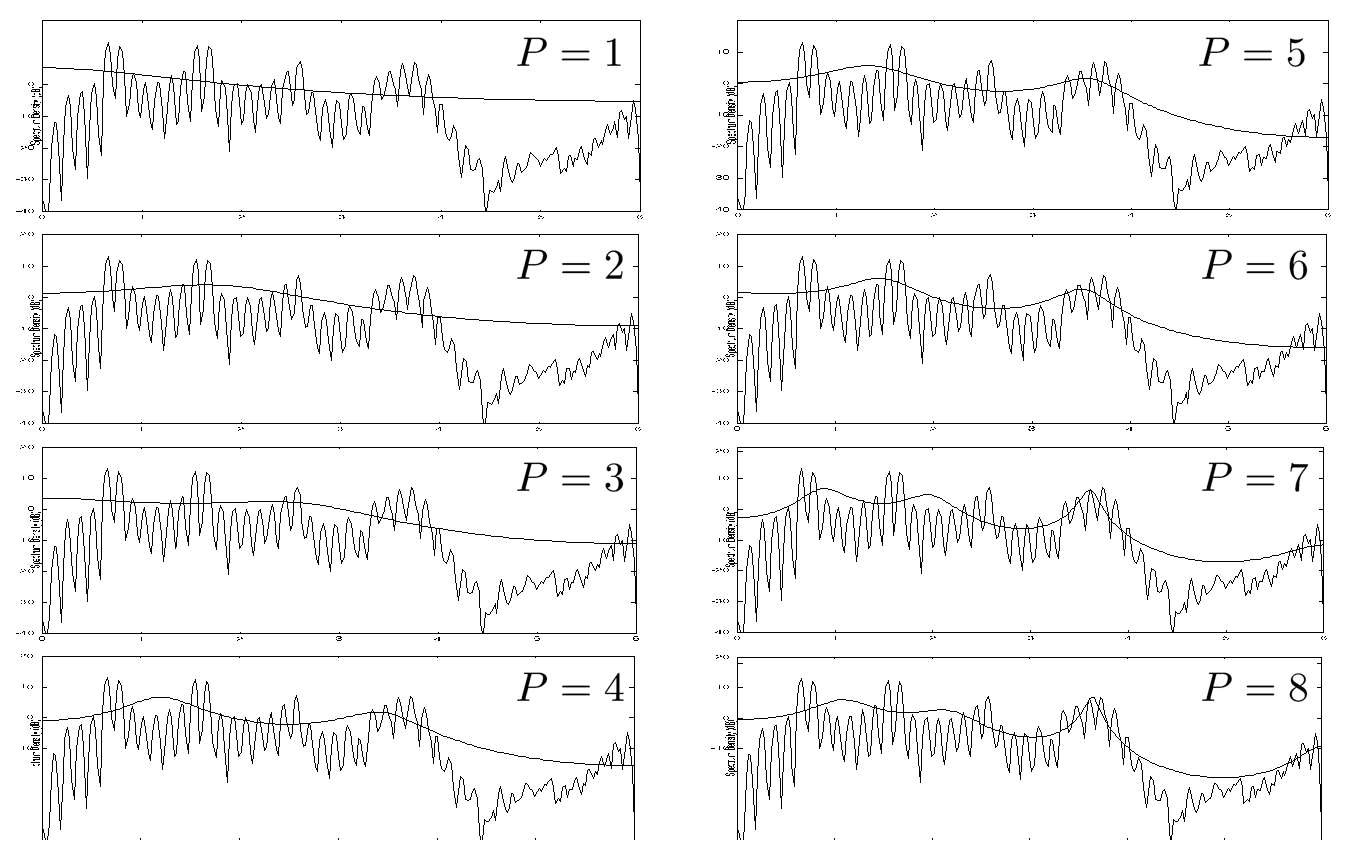
\includegraphics[width=.98\linewidth,keepaspectratio=true]{sections/speech/AllPoleFitting1.eps}
%\caption{音声スペクトルと次数$P$の線形予測分析により推定された全極スペクトル($P=1,\ldots,8$)}
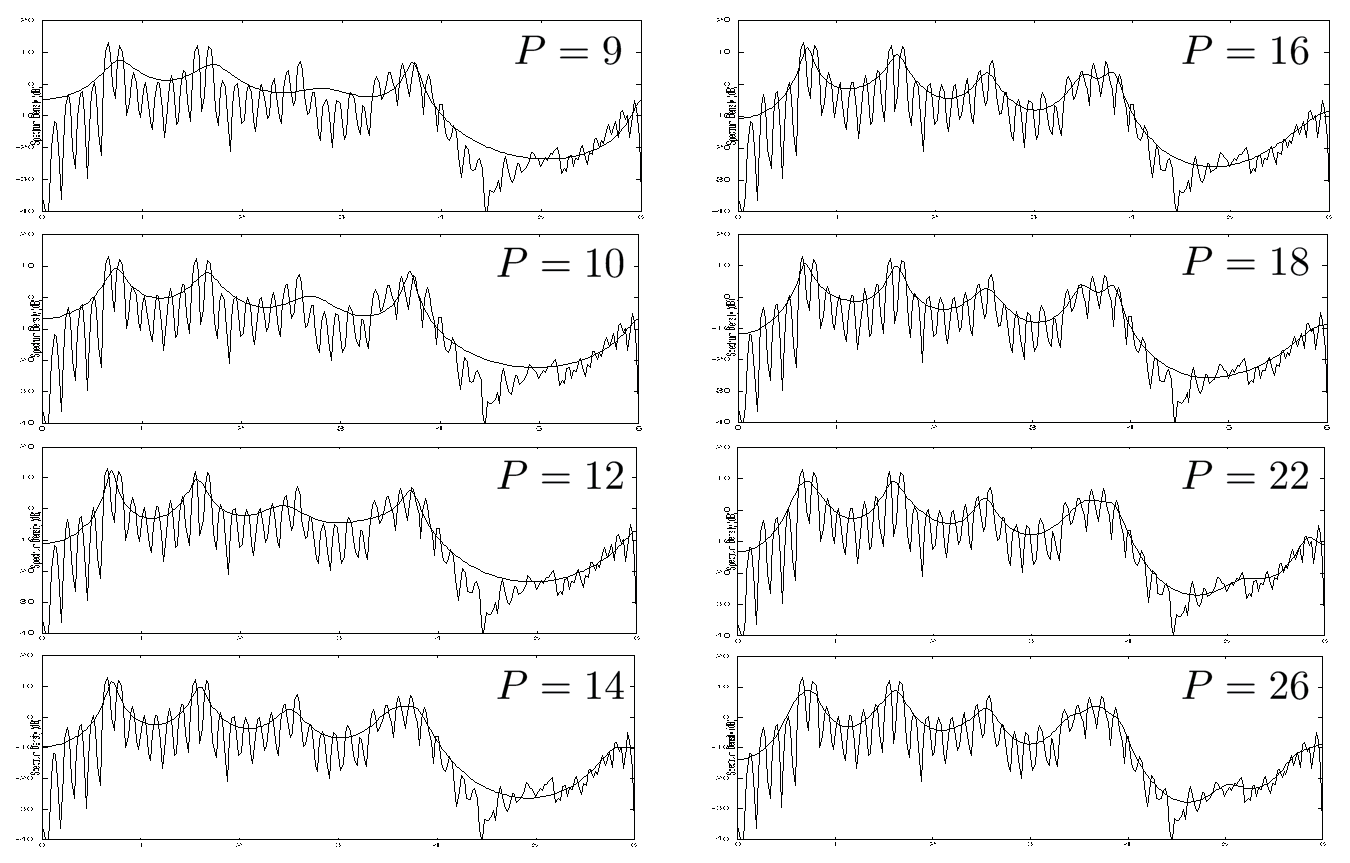
\includegraphics[width=.98\linewidth,keepaspectratio=true]{sections/speech/AllPoleFitting2.eps}
\vspace{0ex}
 \caption{音声スペクトルと次数$P$の線形予測分析により推定された全極スペクトル($P=1,\ldots,8,9,10,12,14,16,18,22,26$)}
\label{fig:AllPoleFitting}
\vspace{0ex}
\end{figure}

\subsection{無損失系等長音響管による声道モデルとしての解釈}
\label{subsec:acoustic_cube_model}

本節では全極システムを仮定することが無損失系等長音響管により声道をモデル化していることに相当することを示します.
%線形予測分析の手法にのみ関心のある読者は本節は読み飛ばしていただいて差し支えありません.
そこでまず,一定の断面積の管の中を進行する音波の波動方程式を導き,
これをもとに,断面積が不連続に変化する管内を音波がどう伝播していくかを考えます.

音波は空気などの媒質の中を伝播する粗密波で,
%粗密波の伝播速度を音速,
平均圧力を基準として音波によって引き起こされる圧力の変化分を音圧といいます.
空間中のある断面に圧力変動が伝わると,その断面上で,媒質を構成する微小粒子が平衡位置から変位させられます.
このときの粒子の速度を粒子速度といいます.
音波は音圧と粒子速度の二つの量によって特徴付けられ,
これらの量を支配する方程式を波動方程式と呼びます.
ここでは,断面積が$S$で$d$軸方向に伸びている管を考え,
この管と$d$と$d+\Delta d$の二つの面で囲まれた微小部分(\reffig{waveq})における
音圧と粒子速度の関係を導くため,
媒質の運動量の保存を表す運動方程式と
質量の保存を表す連続の方程式を導入します.


まず運動方程式を導きます.
時刻$t$における$d$での音圧を$P(t,d)$とすれば$d+\Delta d$での音圧は$P(t,d) + \frac{\partial P(t,d)}{\partial d} \Delta d$となります.
ゆえに,この微小部分には左右逆向きの力$P(t,d)S$と$(P(t,d) + \frac{\partial P(t,d)}{\partial d} \Delta d)S$
が加わるので,その差の力$- \frac{\partial P(t,d)}{\partial d} \Delta d S$により
微小部分の粒子が動かされます.
管内の媒質の密度を$\rho$とすると微小部分の質量は$\rho\Delta d S$になり,さらに
粒子の変位を$\zeta(t,d)$とすると粒子の加速度は$\frac{\partial^2 \zeta(t,d)}{\partial t^2}$になるので,
\begin{align}
-\frac{\partial P(t,d)}{\partial d}\Delta d S = \rho \Delta d S \frac{\partial^2 \zeta(t,d)}{\partial t^2}
\end{align}
という運動方程式を得ます.
この式に粒子速度$v(t,d) = \frac{\partial \zeta(t,d)}{\partial t}$を代入した
\begin{align}
-\frac{\partial P(t,d)}{\partial d} &= \rho \frac{\partial v(t,d)}{\partial t}
\label{eq:moteq}
\end{align}
が音圧と粒子速度の関係を表す一つ目の式となります.

\begin{figure}[t!]
\centering
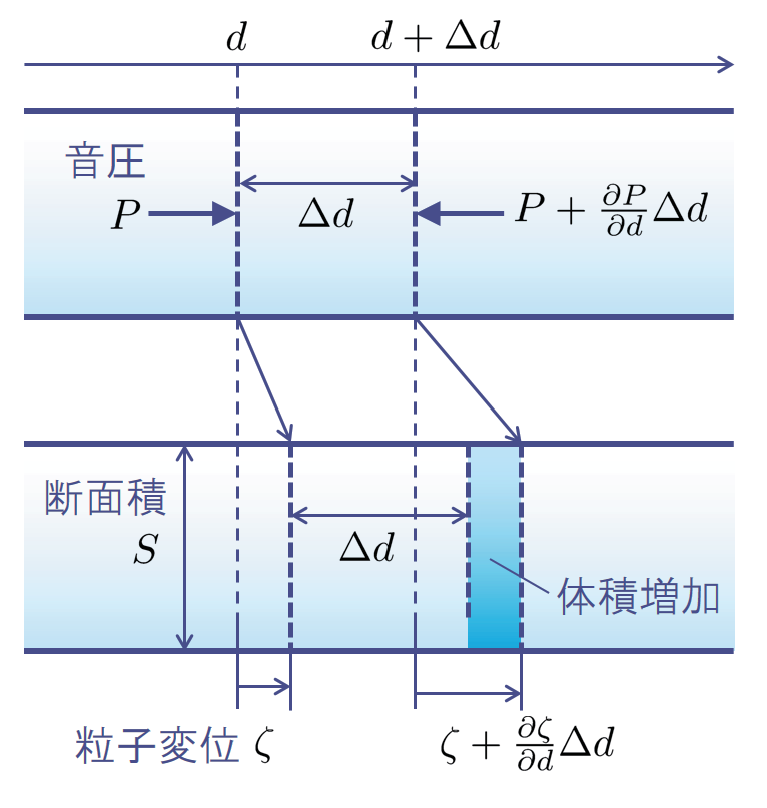
\includegraphics[width=.55\linewidth,keepaspectratio=true]{sections/speech/acoustictube.eps}
\vspace{0ex}
 \caption{***}
\label{fig:waveq}
\vspace{0ex}
\end{figure}


次に連続の方程式を導きます.
上記運動方程式に従って
$d$の位置にあった粒子が$\zeta(t,d)$だけ変位したとすると,$d+\Delta d$にあった粒子
の変位は$\zeta(t,d) + \frac{\partial \zeta(t,d)}{\partial d}\Delta d$となります.
よって,微小部分の体積$\Delta d S$は変位の差と断面積の積
$\frac{\partial \zeta(t,d)}{\partial d}\Delta d S$だけ膨張します.
媒質の体積減少の割合$(\frac{\partial \zeta(t,d)}{\partial d}\Delta d S) / (\Delta d S)$
は加えられた圧力$P(t,d)$に比例するので,比例定数を$K$とすると
\begin{align}
P(t,d) = -K \frac{\partial \zeta(t,d)}{\partial d}
\end{align}
という関係式が得られます.$K$は体積弾性率と呼ばれ,媒質によって決まる値です.
この式の両辺を時間$t$で微分し,粒子速度$v(t,d) = \frac{\partial \zeta(t,d)}{\partial t}$を代入すると
\begin{align}
-\frac{\partial P(t,d)}{\partial t} = K \frac{\partial v(t,d)}{\partial d}
\label{eq:conteq}
\end{align}
という式を得ます.これが連続の方程式で,音圧と粒子速度の関係を表す二つ目の式となります.
%体積速度$u(t,d) = S v(t,s)$

これらの二つの関係式を同時に記述したものが波動方程式です.そこで,両式を統合化することを考えます.
\refeq{moteq}の両辺を$d$で微分した式と\refeq{conteq}の両辺を$t$で微分した式を用いれば,
$v$を消去し$P$だけの式に書き換えることができます.逆に,
\refeq{moteq}の両辺を$t$で微分した式と\refeq{conteq}の両辺を$d$で微分した式を用いることで
$v$だけの式に書き換えることができます.この操作により$P$と$v$に関する波動方程式
\begin{align}
\frac{\partial^2 P(t,d)}{\partial d^2} &= \frac{1}{c^2} \frac{\partial^2 P(t,d)}{\partial t^2}
\\
\frac{\partial^2 v(t,d)}{\partial d^2} &= \frac{1}{c^2} \frac{\partial^2 v(t,d)}{\partial t^2}
\\
c &=\sqrt{\textstyle\frac{K}{\rho}}
\end{align}
を得ます.
%後述するように$c$は音速に対応します.従って,音速$c$は
%媒質の体積弾性率$K$と密度$\rho$によって決まる定数であることが分かります.
これらの式は$P$と$v$の振る舞いを別々に表現したもので,
両者の関係を記述した形にはなっていません.
そこで,$P$と$v$の関係を記述しやすくする目的で
\begin{align}
v(t,d) &=
- \frac{\partial \phi(t,d)}{\partial d}
\label{eq:def_velpot}
\end{align}
を満たす速度ポテンシャルと呼ぶ関数$\phi(t,d)$を導入します.
\refeq{def_velpot}を運動方程式(\refeq{moteq})に代入し,
$d$に関して積分すると
\begin{align}
P(t,d) &=
\rho \frac{\partial \phi(t,d)}{\partial t} + C
\end{align}
を得ます.
ここで,$C$は積分定数ですが,
音波が伝播していない$\phi=0$のとき音圧が$P=0$となるように$C=0$と設定することで
\begin{align}
P(t,d) &=
\rho \frac{\partial \phi(t,d)}{\partial t}
\label{eq:def_velpot2}
\end{align}
を得ます.
\refeqs{def_velpot}{def_velpot2}より,
速度ポテンシャル$\phi(t,d)$は
$P$と$v$を結びつける関数となっていることが分かります.
あとは\refeqs{def_velpot}{def_velpot2}を連続の方程式(\refeq{conteq})に代入することで,
$P$と$v$に関する波動方程式を速度ポテンシャル$\phi(t,d)$を介して
\begin{align}
\frac{\partial^2 \phi(t,d)}{\partial d^2} = 
\frac{1}{c^2}\frac{\partial^2 \phi(t,d)}{\partial t^2} 
\label{eq:waveq}
\end{align}
のように一つの方程式で記述することができます.
***の場合の\refeq{waveq}の解は
\begin{align}
\phi(t,d) = A e^{j\omega(t-d/c)} + B e^{j\omega(t+d/c)}
\end{align}

以上より,一定の断面積の管内を一方向に伝播する音波の波動方程式は
断面積$S$に依存しないことが分かりましたが,以下で
断面積が不連続変化する音響管を伝播する音波の振る舞いを考えるため,
粒子速度$v(t,d)$の代わりに断面積$S$に依存する
体積速度$u(t,d) = S v(t,d)$という量を扱います.

\begin{figure}[t!]
\centering
%\includegraphics[width=.55\linewidth,keepaspectratio=true]{sections/speech/nonuniformacoustictube.eps}
\vspace{0ex}
 \caption{***}
\label{fig:AcousticTubeModel}
\vspace{0ex}
\end{figure}

今,\reffig{AcousticTubeModel}のように
長さが等しく断面積が異なる$M$個の管を連結した非一様音響管を考え,この管内を
長さ方向にのみ伝播する音波を考えます.
$m$番目の区間の管の断面積を$S_m$とすると,この管内を伝播する音波の速度ポテンシャル$\phi_m(t,d)$は
\begin{align}
\frac{\partial^2 \phi_m(t,d)}{\partial d^2} = 
\frac{1}{c^2}\frac{\partial^2 \phi_m(t,d)}{\partial t^2} 
\label{eq:waveq2}
\end{align}
を満たし,一般解は
\begin{align}
\phi_m(t,d) = A e^{j\omega(t-d/c)} + B e^{j\omega(t+d/c)}
\end{align}
で与えられます.
体積速度$u_m(t,d)$と速度ポテンシャル$\phi_m(t,d)$の関係は
\begin{align}
u_m(t,d) &=
- S_m \frac{\partial \phi_m(t,d)}{\partial d}
\label{eq:def_volvel}
\end{align}
で与えられ,
音圧$P_m(t,d)$と速度ポテンシャル$\phi_m(t,d)$の関係は
\refeq{def_velpot2}で与えられるので,
\begin{align}
u_m(t,d) &= u^+_m(t,d) - u^-_m(t,d)
\\
P_m(t,d)&=\frac{\rho c}{S_m}
(u^+_m(t,d) + u^-_m(t,d))
\end{align}
となります.
ただし,$u^+_m(t,d)$, $u^-_m(t,d)$は
\begin{align}
u^+_m(t,d)&=
\frac{j\omega S_m A}{c}e^{j\omega(t-d/c)}
\\
u^-_m(t,d)&=
\frac{j\omega S_m B}{c}e^{j\omega(t+d/c)}
\end{align}
で与えられます.



\section{韻律分析合成}

\subsection{背景と目的}

普段我々私たちは会話をするとき言葉を使って相手にメッセージを伝えますが,言葉とともに声の高低を効果的に使いながら声に表情をつけ,声の調子や意図や,その人っぽさなどのさまざまな情報を相手に伝えています.

声の高低の時間変化を表す基本周波数パターンは大きく分けて
フレーズ成分とアクセント成分と呼ぶ二つの成分からなります.
フレーズ成分とは文や句の全体に及ぶ範囲で緩やかに変化する基本周波数パターンのことで,話者の調子や意図,文の区切りや係り受けを表現するのに重要な役割を担います.
一方,アクセント成分とは各単語の中で急峻に変化する基本周波数パターンのことで,単語の意味や方言の違いに関係します.例えば「はし」という単語は「は」が高い場合と低い場合とでは意味が違いますし,「おいおい」という単語も先頭の「お」が高い場合と低い場合とで意味が違います.特に日本語の場合,単語アクセントと単語の意味の関係は方言によって異なるので,単語内の基本周波数パターンを変えて話せば異なった方言になります.また,フレーズ成分とアクセント成分の大きさは,文や句や単語の強弱を表すいわゆるメリハリに相当します.これらが大きい場合と小さい場合とでは話し方の印象は大きく変わり,メリハリをつけることで発話の中で注目すべき文や単語を相手に示すことができるようになります.以上のように,基本周波数パターンは様々さまざまな情報を持っており,言葉に勝るとも劣らないくらい音声コミュニケーションにおいて大きな役割を果たしています.
基本周波数パターン分析とは,***。

%甲状軟骨による基本周波数制御
基本周波数パターンは声帯を伸縮させる甲状軟骨という部位により制御されています.
藤崎らによってこの制御メカニズムを模擬した物理モデルが提案されており(\reffig{Fujisakimodel}),藤崎モデルと呼ばれています.
甲状軟骨の運動がどのような基本周波数パターンをもたらすかを簡潔に説明した方程式で,日本語を含む多言語の音声の基本周波数パターンを極めて良く表現できることが知られています.このモデルでは,甲状軟骨の二つの独立な運動(並進と回転)に伴う声帯の長さの変化の合計と対数基本周波数の変化が比例関係にあり,それぞれの運動がイントネーションとアクセントに関与しているという仮定がベースとなっています.このモデルに基づき,音声から甲状軟骨がどう動いたかを推定することができれば,その声にそっくりの基本周波数パターンを再現することができ,さらにその数値を変えてやれば甲状軟骨が異なる動きをした場合の基本周波数パターンの音声を再合成することができるようになります.ところが,この逆問題は一筋縄ではいかず長らく未解決問題とされていました.例えば7+3を解くのは簡単でもX+Y=10となるXとYを一意に決められないのと同じで,フレーズ成分とアクセント成分から基本周波数パターンを得る方程式は与えられていたとしても基本周波数パターンのみからフレーズ成分とアクセント成分を一意に決めることはできないからです.しかしまったく全く手がかりがないわけではありません.自然音声におけるフレーズやアクセントのタイミングや強度には統計的な偏りがあります.藤崎モデルの確率モデル化により
統計的アプローチにより基本周波数パターンから藤崎モデルのパラメータを推定する
(フレーズ成分とアクセント成分に分解する)手法が
亀岡らによって提案されています.
\refsubsec{OriginalFujisakiModel}以降で,藤崎モデルについて概説した上で
亀岡らの手法を紹介します.

\subsection{骨格筋の弾性特性}

藤崎モデルでは,
\begin{enumerate}
\item 声帯の伸びの合計と対数基本周波数の変化が比例関係にある
\item 対数基本周波数がフレーズ成分とアクセント成分とベースライン成分の三成分の和で表される
\end{enumerate}
という二つの重要な仮定がベースとなっていました.
これらの仮定の妥当性に対する藤崎による説明は以下のとおりです.

$l$を筋肉の長さとすると,
声帯筋を含む骨格筋において,長さ方向に加わる張力$T$と
剛性${\mbox{d}T}/{\mbox{d}l}$(筋肉を単位長さ変化させるのに必要な力)の間には
\begin{align}
\frac{\mbox{d}T}{\mbox{d}l} = a + b T
\end{align}
のような線形の関係が成り立つことが多くの実測結果により示されています
\cite{Buchthal1944,Sandow1958}.
ただし,$a$は$T=0$における筋肉の剛性です.
声帯筋の静止張力を$T_0$とし,そのときの声帯筋の長さを$l_0$とすると,
この微分方程式より張力$T$と声帯筋の長さ$l$の関係を表す式
\begin{align}
T = \left(T_0 + \frac{a}{b}\right) e^{b(l-l_0)} - \frac{a}{b}
\label{eq:stress-strain}
\end{align}
が導かれます.ここで,$T_0 \gg a/b$のとき,\refeq{stress-strain}は
\begin{align}
T = T_0 e^{b\delta}
\label{eq:stress-strain2}
\end{align}
と近似できます.
ただし,$\delta = l-l_0$は張力が$T_0$から$T$へ変化した際の声帯筋の長さの変化を表します.
一方,一定の張力$T$で張られた密度$\rho$の
弾性膜の固有振動周波数$f_0$は,膜の大きさによって決まる定数$c_0$を用いて
\begin{align}
f_0 = c_0 \sqrt{T/\rho}
\label{eq:F0_tension}
\end{align}
と表されます.
従って,
\refeq{stress-strain2}と\refeq{F0_tension}より,
声帯の伸びが$\delta$のときの基本周波数の対数$y = \log f_0$は
\begin{align}
%f_0 = c_0 \sqrt{T_0 e^{bx} / \rho}%\\
y = \log c_0 \sqrt{T_0/\rho} + \frac{b}{2}\delta
\end{align}
となり,$\delta$と$y$が線形の関係にあることが示されます.
声帯の伸び$\delta$が時間変化する場合,$t$を時刻とすると
基本周波数パターン$y(t)$は
\begin{align}
y(t) &= \log c_0 \sqrt{T_0/\rho} + \frac{b}{2}\delta(t)
\end{align}
のように固定項と時間変化成分
の和として表されます。

声帯の長さは甲状軟骨の平行移動運動と回転運動によって変化します.
平行移動運動によって生じる変化分を$\delta_{\rm p}(t)$,
回転運動によって生じる変化分を$\delta_{\rm a}(t)$とすると,
これらの二つの運動が微小で互いに独立と見なせる範囲では
声帯の長さの変化は$\delta_{\rm p}(t)$と$\delta_{\rm a}(t)$の和
となります.
なお,甲状軟骨の平行移動の時定数は,回転の時定数よりもはるかに大きいため,
多くの言語に共通する特徴として$\delta_{\rm p}(t)$が句単位の比較的緩やかな音調の表現に,
$\delta_{\rm a}(t)$が語または音節単位の比較的急激で局所的な音調の表現に用いられています.


\subsection{基本周波数パターン生成過程モデル\cite{Fujisaki1988}}
\label{subsec:OriginalFujisakiModel}
%\vspace{-1ex}

%ここでは藤崎モデルを概説する。
%藤崎モデルは,音声における$F_0$の対数値の時間軌跡($F_0$パターン)
%を喉頭の生理的,物理的特性に基づいてモデル化したものである。
藤崎モデルでは,
%次のような考え方に基づく。
%甲状軟骨の運動には平行移動と回転の二つの自由度があり,
%それぞれの運動に伴って声帯の長さが変化する。
%声帯の長さの伸びは,これら二つの変化
%の和で表される。
甲状軟骨の二つの独立な運動(平行移動と回転)
に伴う声帯の長さの変化の合計が
$F_0$の時間的変化をもたらす
と解釈され,声帯の伸び
と対数$F_0$の変化が比例関係にあるという仮定
に基づき$F_0$パターンがモデル化されます.


甲状軟骨の平行移動運動に関係する
$F_0$パターンをフレーズ成分,
回転運動に関係する$F_0$パターンを
アクセント成分と呼び,
それぞれ$y_{\rm p}(t)$, $y_{\rm a}(t)$とします。
ただし,$t$は時刻です。
$y_{\rm p}(t)$の生成過程(フレーズ制御機構)
はフレーズ指令と呼ぶ
パルス波を入力とした臨界制動の二次線形系,
$y_{\rm a}(t)$の生成過程(アクセント制御機構)
はアクセント指令と呼ぶ
矩形波を入力とした臨界制動の二次線形系に
より表現されます.
以上の二つの成分と,
声帯の物理的性質によって決まる
ベースライン成分$y_b$の和$y_{\rm p}(t)+y_{\rm a}(t)+y_b$
で$F_0$パターン$y(t)$を表したものが藤崎モデルです.
フレーズ成分は短区間の上昇のあとに緩やかな下降をなす成分で,
アクセント成分は急激な上昇下降をなす成分であるため,
多くの言語に共通して
前者が句単位の比較的緩やかな音調を,
後者が語または音節単位の比較的急激で局所的な
音調を表現する役割を担っていると考えられています.
フレーズ制御機構およびアクセント制御機構は
\begin{align}
G_{\rm p}(t)&=
\begin{cases}
\alpha^2 t e^{-\alpha t}&(t\ge 0)\\
0&(t<0)
\end{cases}
%\nonumber
%\end{align}
\\
%\begin{align}
G_{\rm a}(t)&=
\begin{cases}
\beta^2 t e^{-\beta t}&(t\ge 0)\\
0&(t<0)
\end{cases}
\end{align}
で与えられる
インパルス応答$G_{\rm p}(t)$, $G_{\rm a}(t)$によって
特徴づけられます.
$\alpha$と$\beta$はそれぞれの制御機構
の固有角周波数であるが,これらは話者ごとにほぼ一定値を
とること,話者の個人差も言語による差も比較的小さい
ことが確かめられており,
おおよそ$\alpha\!=\!3$rad/s, $\beta\!=\!20$rad/s
程度であることが経験的に知られています.
これらを用いて$F_0$パターン$y(t)$は具体的に
\begin{align}
\hspace{-0.0cm}
y(t) = y_{\rm b}
&+\sum_{i}A_{{\rm p},i}G_{\rm p}(t-T_{0,i})
\nonumber
\\
&+\sum_{j}A_{{\rm a},j}
\big\{S_{\rm a}(t-T_{1,j})-S_{\rm a}(t-T_{2,j})\big\}
%\nonumber
\end{align}
と表されます.
%(\reffig{fujisaki_model})
ただし,$A_{{\rm p},i}$と$T_{0,i}$は
それぞれ$i$番目のフレーズ指令の大きさと生起時刻であり,
$A_{{\rm a},j}$と$T_{1,j}$,と$T_{2,j}$は
それぞれ$j$番目のアクセント指令の振幅と始端時刻と
終端時刻を表します.
ところで,
アクセント制御機構のインパルス応答
$G_{\rm a}(t)$は$S_{\rm a}(t)$
の時間微分ゆえ
\begin{align}
G_{\rm a}(t)=
\begin{cases}
\beta^2 t e^{-\beta t}&(t\ge 0)\\
0&(t<0)
\end{cases}
\end{align}
となり,$G_{\rm p}(t)$と同形であることが分かります.
従って,アクセント成分$y_{\rm a}(t)$は複数の矩形波からなるアクセント指令関数$u_{\rm a}(t)$
と$G_{\rm a}(t)$の畳み込みによって表されます.

%\begin{figure}[t!]
%\centering
%\includegraphics[width=.98\linewidth,keepaspectratio=true]{sections/speech/fujisakimodel_ver3_ill.eps}
%\vspace{-1ex}
% \caption{Block diagram of Fujisaki model}
%\label{fig:fujisaki_model}
%\vspace{-2ex}
%\end{figure}


%\subsection{藤崎モデルの離散時間表現}
%\label{sec:DiscreteFujisaki}


本章では,藤崎モデルの離散時間表現を得るため,
連続時間システムのフレーズ制御機構およびアクセント制御機構
に対して後退差分変換により離散化を行います.
%離散化することの理由はのちに明らかにする。
まず,フレーズ制御機構の伝達関数(Laplace変換)は
$%\begin{align}
\mathcal{G}_{\rm p}(s)= 
\mathcal{L}\big[G_{\rm p}(t)\big]=
{\alpha^2}/{(s+\alpha)^2}
$%\end{align}
で与えられます.
後退差分変換は,
時間微分演算子$s$
を$z$領域における後退差分演算子
$
s\simeq
{(1-z^{-1})}/{t_{0}}
$
に置き換える変換であり($t_0$は変換先の離散時間表現における
サンプリング周期),
この変換により,
$\mathcal{G}^{-1}_{\rm p}(s)$
の逆システムの伝達関数を$z$領域で
\begin{align}
\mathcal{H}_{\rm p}^{-1}(z)&= 
a_2
%\frac{1}{\alpha^2t_{0}^2}
z^{-2}
+a_1
%-\frac{2(\alpha t_{0} +1)}{\alpha^2t_{0}^2}
z^{-1}
+a_0
%+\frac{(\alpha t_{0}+1)^2}{\alpha^2t_{0}^2}.
\end{align}
と書くことができます.
ただし,
\begin{align}
a_2 = (\psi-1)^2,~~
a_1 = -2\psi(\psi-1),~~
a_0 = \psi^2
\label{eq:a_psi}
\end{align}
および,$\psi = 1+1/(\alpha t_0)$です.
ここで,$k$を離散時刻インデックスとし,
フレーズ指令関数およびフレーズ成分の
離散時間表現をそれぞれ
$u_{\rm p}[k]$および$y_{\rm p}[k]$
とすると,$y_{\rm p}[k]$
は,単一のパラメータ$\psi$(あるいは$\alpha$)
によって特性が決まる拘束つき全極モデルからの出力
\begin{align}
&u_{\rm p}[k] = a_0 y_{\rm p}[k]+a_1y_{\rm p}[k-1]+a_2y_{\rm p}[k-2]
\end{align}
と見なすことができます.
同様に,
アクセント指令関数$u_{\rm a}[k]$
とアクセント成分$y_{\rm a}[k]$の関係も
\begin{align}
u_{\rm a}[k] &= b_0 y_{\rm a}[k]+b_1y_{\rm a}[k-1]+b_2y_{\rm a}[k-2]
\end{align}
と書くことができます.
ただし,
$b_2 = (\varphi-1)^2$, $b_1 = -2\varphi(\varphi-1)$,
$b_0 = \varphi^2$, 
$\varphi = 1+1/(\beta t_0)$
です.
ベースライン成分$y_{\rm b}(t)$の離散時間表現
を$y_{\rm b}[k]$とすると,
藤崎モデルの離散時間表現はこれらの三成分の和
$y[k]=y_{\rm p}[k]+y_{\rm a}[k]+y_{\rm b}[k]$
で与えられます.


%\subsection{藤崎モデルの確率モデル化}

次に,${u}_{\rm p}[k]$と${u}_{\rm a}[k]$をモデル化します.
藤崎モデルにおいて,フレーズ指令とアクセント指令に関して
以下のような規則が定められています.

(A1) フレーズ指令はパルス波,
アクセント指令は矩形波である。
(A2) 発話の開始または先行フレーズ内のアクセント指令終了後に
フレーズ指令が発生する。また,フレーズ指令の後にアクセント開始指令が発生する。
つまり,アクセント指令発生中はフレーズ指令は発生しない。
(A3) アクセント指令の開始した後には必ずアクセント終了指令が発生する。
つまり,隣接するアクセント指令同士は重なり合うことはない。
%\begin{enumerate}
%\item フレーズ指令はパルス波,
%アクセント指令は矩形波である。
%\item 発話の開始または先行フレーズ内のアクセント指令終了後に
%フレーズ指令が発生する。また,フレーズ指令の後にアクセント開始指令が発生する。
%つまり,アクセント指令発生中はフレーズ指令は発生しない。
%\item アクセント指令の開始した後には必ずアクセント終了指令が発生する。
%つまり,隣接するアクセント指令同士は重なり合うことはない。
%\end{enumerate}

%よって,${u}_{\rm p}[k]$, ${u}_{\rm a}[k]$には
%上記のような規則を反映した制約が必要である。
藤崎モデルのパラメータ推定における難しさの一つは,
これらの制約の下で最適推定をいかにして行えるかという
点にあろう。
特に,上記の(A2), (A3)より,${u}_{\rm p}[k]$と${u}_{\rm a}[k]$
は相互に依存し合う関係がある点に注意が必要である。
提案法では,これを解決するため隠れマルコフモデル(HMM)を用いて
指令入力信号を確率モデル化する。まず,
$\Vec{o}[k]:=({u}_{\rm p}[k], {u}_{\rm a}[k])^{\rm T}$
を,
\begin{align}
&\Vec{o}[k]\sim\mathcal{N}
\left(\Vec{\nu}[k],\Vec{\Upsilon}\right)
\label{eq:TimeVaryingGauss}
\\
&\Vec{\nu}[k]:=
\begin{bmatrix}
\mu_{\rm p}[k]\\
\mu_{\rm a}[k]
\end{bmatrix}
,~~
\Vec{\Upsilon}:=
\begin{bmatrix}
\sigma_{\rm p}^2&0\\
0&\sigma_{\rm a}^2
\label{eq:TimeVaryingGauss2}
\end{bmatrix}
\end{align}
のように正規分布する確率変数と見なし,
平均$\Vec{\nu}[k]$
が\reffig{command_model}のような
状態遷移に伴って変化するモデルを考える。
これはHMMに他ならず,
このように$\Vec{o}[k]$を
HMMでモデル化したことにより,
状態遷移の経路制限(状態遷移確率の設定)を通して
$\Vec{\nu}[k]$に対して上記の(A1)~(A3)を
満たすような制約を与えることが可能となる。
提案するHMMの構成は以下のとおりである。

%\medskip
%\begin{figure}[t]
\noindent
\begin{center}
\fbox{
\hspace{-0.1cm}
\begin{tabular}{rl}
出力値系列:&\!\!\!\!$\{\Vec{o}[k]\}_{k=1}^{K}$\\
状態集合:&\!\!\!\!$\mathcal{S}:=\{{\rm p}_0,{\rm p}_1,{\rm a}_0,\cdots,{\rm a}_{N}\}$\\
状態系列:&\!\!\!\!$\{s_{k}\}_{k=1}^{K}$\\
状態出力分布:&\!\!\!\!
$P(\Vec{o}[k]|s_{k}=i)=
%\Vec{o}[k]|s[k]=k\sim
\mathcal{N}(\Vec{c}_i[k],\Mat{\Upsilon})$\\
&
%\hspace{-0.0cm}
\!\!\!\!
$\Vec{c}_{i}[k]\!=\!\!
%\begin{bmatrix}
%c_{\rm p}^{(i)}\![k]\\
%c_{\rm a}^{(i)}
%\end{bmatrix}
%\!\!=\!
\begin{cases}
\big(0, 0\big)^{\!\rm T}&\hspace{-0.25cm}(i\!=\!{\rm p}_0,{\rm a}_0)\\
\big(A_{{\rm p}}[k],0\big)^{\!\rm T}&\hspace{-0.25cm}(i\!=\!{\rm p}_1)\\
%\big(0, 0\big)^{\!\rm T}&\hspace{-0.25cm}(i\!=\!{\rm a}_0)\\
\big(0,A_{{\rm a}}^{(n)}\big)^{\!\rm T}&\hspace{-0.25cm}(i\!=\!{\rm a}_n)
\end{cases}
$\\
状態遷移確率:&\!\!\!\!
$\phi_{i',i}:=\log P(s_{k}=i|s_{k-1}=i')$
\end{tabular}
}
\end{center}
%\end{figure}
%\medskip


簡単のため状態遷移確率を定数とすると,
以上より指令入力モデルにおいて推定すべきパラメータは,
フレーズ指令の大きさ$A_{\rm p}[k]$,状態遷移系列$s_{k}$,
アクセント指令の大きさ$\{A_{\rm a}^{(n)}\}_{n=1}^{N}$,
指令入力信号の分散$\sigma_{\rm p}^2,\sigma_{\rm a}^2$
であり,これらをまとめて$\theta_{u}$
%\begin{align}
%\theta_{u}:=\big\{\{A_{\rm p}[k],s[k]\}_{k=1}^{K},\{A_{\rm a}^{(n)}\}_{n=1}^{N},\sigma_{\rm p}^2,\sigma_{\rm a}^2\big\}
%\end{align}
と記す。また,平均値系列$\{\mu_{\rm p}[k]\}_{k=1}^{K}$および
$\{\mu_{\rm a}[k]\}_{k=1}^{K}$は,
状態遷移系列$\{s_{k}\}_{k=1}^{K}$が与えられたもとで
$
(
\mu_{\rm p}[k], 
\mu_{\rm a}[k]
)^{\rm T}
\leftarrow
\Vec{c}_{s_{k}}[k]
%,~~(k=1,\cdots,K)
%\label{eq:map_to_mu}
$
で与えられる。

\begin{figure}[t]
\centering
%\includegraphics[width=.98\linewidth,keepaspectratio=true]{Command_model_english_ver2.eps}
\vspace{-1ex}
 \caption{Command function modeling with HMM.}
\label{fig:command_model}
\vspace{-3ex}
\end{figure}



%\subsection{尤度関数と事前確率}

前述の指令入力モデルに基づき
$\Vec{y}=({y}[1],\cdots,y[K])^{\rm T}$の確率密度関数を導く。
\refeqs{TimeVaryingGauss}{TimeVaryingGauss2}より,
$\Vec{u}_{\rm p}$ $:=({u}_{\rm p}[1],$ $\cdots,{u}_{\rm p}[K])^{\rm T}$\!, 
$\Vec{u}_{\rm a}:=({u}_{\rm a}[1],\cdots,{u}_{\rm a}[K])^{\rm T}$\!, 
$\Vec{\mu}_{\rm p}:=$ $({\mu}_{\rm p}[1],$ $\cdots,{\mu}_{\rm p}[K])^{\rm T}$\!, 
$\Vec{\mu}_{\rm a}:=({\mu}_{\rm a}[1],\cdots,{\mu}_{\rm a}[K])^{\rm T}$\!
とすると,
\begin{align}
\Vec{u}_{\rm p}|\theta_u\sim
\mathcal{N}(
\Vec{\mu}_{\rm p},
\Mat{\Sigma}_{\rm p}
),~~\Mat{\Sigma}_{\rm p}=\sigma_{\rm p}^2\Mat{I}
\label{eq:u_p_dist}
\\
\Vec{u}_{\rm a}|\theta_u\sim
\mathcal{N}(
\Vec{\mu}_{\rm a},
\Mat{\Sigma}_{\rm a}
),~~\Mat{\Sigma}_{\rm a}=\sigma_{\rm a}^2\Mat{I}
\label{eq:u_a_dist}
\end{align}
が言える。
\refsec{DiscreteFujisaki}で得た関係式より,
フレーズ成分$\Vec{y}_{\rm p}:=(y_{\rm p}[1],$ $\cdots,$ $y_{\rm p}[K])^{\rm T}$
と$\Vec{u}_{\rm p}$の関係,
および,アクセント成分$\Vec{y}_{\rm a}:=(y_{\rm a}[1],$ $\cdots,$ $y_{\rm a}[K])^{\rm T}$
と$\Vec{u}_{\rm a}$の関係は,
\begin{align}
\!\!
\Mat{A}\!:=\!
\begin{bmatrix}
%\hspace{0.1cm}
a_0&\hspace{-0.3cm} &\hspace{-0.3cm} &\hspace{-0.3cm}&\hspace{-0.3cm}O\vspace{-0.1cm}\\
a_1&\hspace{-0.3cm}a_0&\hspace{-0.3cm} &\hspace{-0.3cm} &\hspace{-0.3cm}\vspace{-0.1cm}\\
a_2&\hspace{-0.3cm}a_1&\hspace{-0.3cm}a_0&\hspace{-0.3cm}&\hspace{-0.3cm}\vspace{-0.1cm}\\
 &\hspace{-0.3cm}\ddots&\hspace{-0.3cm}\ddots&\hspace{-0.3cm}\ddots&\hspace{-0.3cm}\vspace{-0.1cm}\\
O&\hspace{-0.3cm} &\hspace{-0.3cm}a_2 &\hspace{-0.3cm}a_1 &\hspace{-0.3cm}a_0~
\end{bmatrix}
\!,~~
\Mat{B}\!:=\!
\begin{bmatrix}
%\hspace{0.1cm}
b_0&\hspace{-0.3cm} &\hspace{-0.3cm} &\hspace{-0.3cm}&\hspace{-0.3cm}O\vspace{-0.1cm}\\
b_1&\hspace{-0.3cm}b_0&\hspace{-0.3cm} &\hspace{-0.3cm} &\hspace{-0.3cm}\vspace{-0.1cm}\\
b_2&\hspace{-0.3cm}b_1&\hspace{-0.3cm}a_0&\hspace{-0.3cm}&\hspace{-0.3cm}\vspace{-0.1cm}\\
 &\hspace{-0.3cm}\ddots&\hspace{-0.3cm}\ddots&\hspace{-0.3cm}\ddots&\hspace{-0.3cm}\vspace{-0.1cm}\\
O&\hspace{-0.3cm} &\hspace{-0.3cm}b_2 &\hspace{-0.3cm}b_1 &\hspace{-0.3cm}b_0~
\end{bmatrix}\!
\!\!
%\nonumber
\end{align}
と置くと,それぞれ
$%\begin{align}
\Vec{u}_{\rm p}=\Vec{A}\Vec{y}_{\rm p},~
\Vec{u}_{\rm a}=\Vec{B}\Vec{y}_{\rm a}
$%\end{align}
のように表現できることから,\refeqs{u_p_dist}{u_a_dist}より
\begin{align}
\Vec{y}_{\rm p}|\theta_u,\alpha&\sim\mathcal
{N}\big(
\Mat{A}^{-1}\Vec{\mu}_{\rm p},
\Mat{A}^{-1}\Mat{\Sigma}_{\rm p}
(\Mat{A}^{-1})^{\rm T}
\big)
\label{eq:y_p_dist}
\\
\Vec{y}_{\rm a}|\theta_u,\beta&\sim\mathcal{N}\big(
\Mat{B}^{-1}\Vec{\mu}_{\rm a},
\Mat{B}^{-1}\Mat{\Sigma}_{\rm a}
(\Mat{B}^{-1})^{\rm T}
\big)
\label{eq:y_a_dist}
\end{align}
が導かれる。
ベース成分$y_{\rm b}[k]$についても,同様に
白色Gauss性雑音$\epsilon_{\rm b}[k]$
に起因する確率変数
$y_{\rm b}[k] = \mu_{\rm b} + \epsilon_{\rm b}[k]$
と仮定し,
$\epsilon_{\rm b}[k]\sim\mathcal{N}(0,\sigma_{\rm b}^2)$
とし,同様に,
$\epsilon_{\xi}[j]$と
$\epsilon_{\xi'}[j']$は
$(\xi,j)\neq(\xi',j')$
のとき独立とすると,
\begin{align}
\Vec{y}_{\rm b}|\mu_{\rm b}\sim
\mathcal{N}
(\mu_{\rm b}\Vec{1},\Mat{\Sigma}_{\rm b})
\label{eq:y_b_dist}
\end{align}
が言える。ただし,$\Mat{\Sigma}_{\rm b}=\sigma_{\rm b}^2\Mat{I}$
であり,$\theta_{\rm b}:=\{\mu_{\rm b},\sigma_{\rm b}^2\}$と置く。
仮定より,$\Vec{y}_{\rm p}$, $\Vec{y}_{\rm a}$, $\Vec{y}_{\rm b}$
は独立なので,
$\Theta:=\{\theta_u$, $\alpha$, $\beta$, $\theta_{\rm b}\}$
が与えられたもとでの
$F_0$パターン$\Vec{y}=\Vec{y}_{\rm p}+\Vec{y}_{\rm a}+\Vec{y}_{\rm b}$
の確率密度関数は,
\refeqs{y_p_dist}{y_a_dist}と\refeq{y_b_dist}
より,
\begin{multline}
\Vec{y}|\Theta\sim
\mathcal{N}
\big(
\Mat{A}^{-1}\Vec{\mu}_{\rm p}
+
\Mat{B}^{-1}\Vec{\mu}_{\rm a}
+\mu_{\rm b}\Vec{1}
,
\\
\Vec{A}^{-1}\Vec{\Sigma}_{\rm p}(\Vec{A}^{-1})^{\rm T}
+
\Mat{B}^{-1}\Mat{\Sigma}_{\rm a}(\Mat{B}^{-1})^{\rm T}
+
\Mat{\Sigma}_{\rm b}
\big)
\end{multline}
で与えられる。
以上より,
\begin{align}
P(\Vec{y}|{\Theta})
&=
\frac{|\Mat{\Sigma}^{-1}|^{1/2}}{(2\pi)^{T/2}}
\exp
\left\{
-\frac{1}{2}
(\Vec{y}-\Vec{\mu})^{\rm T}
\Mat{\Sigma}^{-1}
(\Vec{y}-\Vec{\mu})
\right\}
\nonumber\\
\Vec{\mu}&=\Mat{A}^{-1}\Vec{\mu}_{\rm p}+\Mat{B}^{-1}\Vec{\mu}_{\rm a}+\mu_{\rm b}\Vec{1}
\label{eq:likelihood_fujisaki}
\\
\Mat{\Sigma}&=
\Mat{A}^{-1}
\Mat{\Sigma}_{\rm p}
\big(\Mat{A}^{\rm T}\big)^{-1}
+
\Mat{B}^{-1}
\Mat{\Sigma}_{\rm a}
\big(\Mat{B}^{\rm T}\big)^{-1}
+
\Mat{\Sigma}_{\rm b}
\nonumber
\end{align}
が,$F_0$パターン$\Vec{y}$が与えられたときの
藤崎モデルパラメータ$\Theta$の尤度関数である。

$\Theta$の事前確率については,各要素は独立で,
状態遷移系列$\{s[k]\}_{k=1}^{K}$と
制御パラメータの$\psi$と$\varphi$
以外のパラメータは一様に分布すると仮定し,
$P(\Theta)\propto
P(\psi)
P(\varphi)
P(s_{1})\prod_{k=2}^{K}
P(s_{k}|s_{k-1})$
とする。

%\subsection{パラメータ推定アルゴリズム}
%\label{sec:optimization}



$P(\Theta|\Vec{y})$を最大化する問題(\refeq{analysis_step}に相当)
は解析的に解くことはできないが,
$\Vec{x}:=$
$(\Vec{y}_{\rm p}^{\rm T}$,
$\Vec{y}_{\rm a}^{\rm T}$,
$\Vec{y}_{\rm b}^{\rm T})^{\rm T}$
を完全データと見なすことで
EMアルゴリズムによる不完全データ問題に帰着できる。
この場合,
完全データの対数尤度は,先に見たとおり,
\begin{align}
\log
P(\Vec{x}|{\Theta})
&\mathop{=}^{\rm c}
\frac{1}{2}\log |\Mat{\Lambda}^{-1}|
-\frac{1}{2}
(\Vec{x}-\Vec{m})^{\rm T}
\Mat{\Lambda}^{-1}
(\Vec{x}-\Vec{m})
\nonumber\\
\Vec{x}&:=
\begin{bmatrix}
\Vec{y}_{\rm p}\\
\Vec{y}_{\rm a}\\
\Vec{y}_{\rm b}
\end{bmatrix},~
\Vec{m}:=
\begin{bmatrix}
\Mat{A}^{-1}\Vec{\mu}_{\rm p}\\
\Mat{B}^{-1}\Vec{\mu}_{\rm a}\\
\mu_{\rm b}\Vec{1}
\end{bmatrix}\\
\Mat{\Lambda}^{-1}&:=
\begin{bmatrix}
\Mat{A}^{\rm T}
\Mat{\Sigma}_{\rm p}^{-1}
\Mat{A}
&\Vec{O}&\Vec{O}\\
\Vec{O}&\Mat{B}^{\rm T}
\Mat{\Sigma}_{\rm a}^{-1}
\Mat{B}&\Vec{O}\\
\Vec{O}&\Vec{O}&\Vec{\Sigma}_{\rm b}^{-1}
\end{bmatrix}
\end{align}
で与えられる。
このとき,Q関数$Q({\Theta},{\Theta}')$は,
\begin{multline}
Q({\Theta},{\Theta}')
\mathop{=}^{\rm c}
\frac{1}{2}
\Big[
\log |\Mat{\Lambda}^{-1}|
-
\mbox{tr}
(
\Mat{\Lambda}^{-1}\mathbb{E}[\Vec{x}\Vec{x}^{\rm T}|\Vec{y};\Theta']
)
\\
+2\Vec{m}^{\rm T}\Mat{\Lambda}^{-1}\mathbb{E}[\Vec{x}|\Vec{y};\Theta']
-\Vec{m}^{\rm T}\Mat{\Lambda}^{-1}\Vec{m}
\Big]
+\log P(\Theta)
\!\!\!\!
\end{multline}
となる。ここで,
$\Vec{y}=\Mat{H}\Vec{x}$(ただし,$\Mat{H}=[\Mat{I}~\Mat{I}~\Mat{I}]$)であるから,
$\mathbb{E}[\Vec{x}|\Vec{y};\Theta]$と
$\mathbb{E}[\Vec{x}\Vec{x}^{\rm T}|\Vec{y};\Theta]$は,具体的に
\begin{align}
\hspace{-0.2cm}
\mathbb{E}[\Vec{x}|\Vec{y};\Theta]&=
\Vec{m}+\Mat{\Lambda}\Mat{H}^{\rm T}
(\Mat{H}\Mat{\Lambda}\Mat{H}^{\rm T})^{-1}
(\Vec{y}\!-\!\Mat{H}\Vec{m})
\!\!\
\label{eq:estep_mean}
\\
%&=
%\Vec{m}+
%\Mat{\Gamma}(\Vec{y}-\Vec{\mu})
%\\
\hspace{-0.2cm}
\mathbb{E}[\Vec{x}\Vec{x}^{\rm T}|\Vec{y};\Theta]
&=
\Mat{\Lambda}-
\Mat{\Lambda}\Mat{H}^{\rm T}(\Mat{H}\Mat{\Lambda}\Mat{H}^{\rm T})^{-1}
\Mat{H}\Mat{\Lambda}
\nonumber\\
&~~~~~~~~~~~~~~~~~+
\mathbb{E}[\Vec{x}|\Vec{y};\Theta]
\mathbb{E}[\Vec{x}|\Vec{y};\Theta]^{\rm T}
\label{eq:estep_var}
\end{align}
と書ける。Eステップでは,直前のステップで更新されたモデルパラメータを
$\Theta'$に代入し,上記に基づいて
$\mathbb{E}[\Vec{x}|\Vec{y};\Theta']$と
$\mathbb{E}[\Vec{x}\Vec{x}^{\rm T}|\Vec{y};\Theta']$
が算出される。
$\Vec{y}_{\rm p}$, $\Vec{y}_{\rm a}$, $\Vec{y}_{\rm b}$に対応するように
$\mathbb{E}[\Vec{x}|\Vec{y};\Theta']$および
$\mathbb{E}[\Vec{x}\Vec{x}^{\rm T}|\Vec{y};\Theta']$を
\begin{align}
\mathbb{E}[\Vec{x}|\Vec{y};\Theta']\!=\!
\begin{bmatrix}
\bar{\Vec{x}}_{\rm p}\\
\bar{\Vec{x}}_{\rm a}\\
\bar{\Vec{x}}_{\rm b}
\end{bmatrix}\!,~~
\mathbb{E}[\Vec{x}\Vec{x}^{\rm T}|\Vec{y};\Theta']
\!=\!
\begin{bmatrix}
\Vec{R}_{\rm p}&\hspace{-0.3cm}* &\hspace{-0.3cm}*\\
* &\hspace{-0.3cm}\Vec{R}_{\rm a}&\hspace{-0.3cm}*\\
*&\hspace{-0.3cm}*&\hspace{-0.3cm}\Vec{R}_{\rm b}
\end{bmatrix}\!\!
\end{align}
のように区分表現すると,Q関数は
\begin{small}
\begin{align}
Q({\Theta},{\Theta}')&\mathop{=}^{c}
\frac{1}{2}
\Big[
\log|\Mat{A}^{\rm T}\Mat{\Sigma}_{\rm p}^{-1}\Mat{A}|
+
\log|\Mat{B}^{\rm T}\Mat{\Sigma}_{\rm a}^{-1}\Mat{B}|
+
\log|\Mat{\Sigma}_{\rm b}^{-1}|
\nonumber\\
&-{\rm tr}(\Mat{A}^{\rm T}\Mat{\Sigma}_{\rm p}^{-1}\Mat{A}\Mat{R}_{\rm p})
+2\Vec{\mu}_{\rm p}^{\rm T}\Mat{\Sigma}_{\rm p}^{-1}\Mat{A}\bar{\Vec{x}}_{\rm p}
-\Vec{\mu}_{\rm p}^{\rm T}\Mat{\Sigma}_{\rm p}^{-1}\Vec{\mu}_{\rm p}
\nonumber\\
&-
{\rm tr}(\Mat{B}^{\rm T}\Mat{\Sigma}_{\rm a}^{-1}\Mat{B}\Mat{R}_{\rm a})
+2\Vec{\mu}_{\rm a}^{\rm T}\Mat{\Sigma}_{\rm a}^{-1}\Mat{B}\bar{\Vec{x}}_{\rm a}
-\Vec{\mu}_{\rm a}^{\rm T}\Mat{\Sigma}_{\rm a}^{-1}\Vec{\mu}_{\rm a}
\nonumber\\
&-{\rm tr}(\Vec{\Sigma}_{\rm b}^{-1}\Vec{R}_{\rm b})
+2\Vec{\mu}_{\rm b}^{\rm T}\Mat{\Sigma}_{\rm b}^{-1}\bar{\Vec{x}}_{\rm b}
-\Vec{\mu}_{\rm b}^{\rm T}\Mat{\Sigma}_{\rm b}^{-1}\Vec{\mu}_{\rm b}
\Big]
\nonumber\\
+&\log P(\Theta)
\!\!
\end{align}
\end{small}
と書き直せて,これを用いて各パラメータについて
Mステップの更新式を求めることができる。

\medskip
\noindent
{\bf 1) 状態系列:}
Q関数の中で$s\!:=\!\{s_k\}_{k=1}^{K}$に関係する項は
\begin{align}
\mathcal{I}_1(s):=
&
-\frac{1}{2}
\sum_{k=1}^{K}
({\Vec{o}}[k]-\Vec{c}_{s_k}[k])^{\rm T}
\Mat{\Upsilon}^{-1}
({\Vec{o}}[k]-\Vec{c}_{s_k}[k])
\nonumber\\
&+\log P(s_{1}) + \sum_{k=2}^{K}\log P(s_k|s_{k-1})
\end{align}
となる。ただし,
$
\Vec{o}[k]:=
(
[
\Mat{A}\bar{\Vec{x}}_{\rm p} 
]_{k},
[
\Mat{B}\bar{\Vec{x}}_{\rm a} 
]_{k}
)^{\rm T}
$であり,$[\cdot]_k$はベクトルの$k$番目の要素を表す。
これを最大化する状態遷移系列$\{s_{k}\}_{k=1}^{K}$は
動的計画法により効率的に解くことができる。
まず,すべての状態$i$について
$\delta_{1}(i)$を
$%\begin{align}
\delta_{1}(i) = 
-\frac{1}{2}
(\Vec{o}[1]-\Vec{c}_{i}[1])^{\rm T}
\Mat{\Upsilon}^{-1}
(\Vec{o}[1]-\Vec{c}_{i}[1])
$%\end{align}
と置くと,
$k=2,\cdots,K$について逐次的に
$\delta_{k}(i)$を
$\delta_{k}(i)=
\max_{i'}
\big[
\delta_{k-1}(i')
-\frac{1}{2}
(\Vec{o}[k]-\Vec{c}_{i}[k])^{\rm T}
\Mat{\Upsilon}^{-1}
(\Vec{o}[k]-\Vec{c}_{i}[k])
+\phi_{i'\!,i}
\big]$
により計算していくことができる。
各ステップで選択される状態番号
$\Psi_{k}(i)\!=\!
\argmax_{i'}
[
\delta_{k-1}(i')
+\phi_{i'\!,i}
]$
を記憶しておくことで,
$k=K$まで到達後に
$s_{k-1}\!=\!\Psi_{k}(s_{k})~(k\!=\!K,\cdots,2)$
により選択された状態番号を辿っていくことができ,
最適経路$s_1,\cdots,s_K$を得ることができる。

\medskip
\noindent
{\bf 2) フレーズ制御パラメータ:}
$\psi$の事前分布を
$\psi\sim\mathcal{N}(\mu_{\psi},1/\nu_{\psi}^2)$とする。
\begin{comment}
\begin{align}
\Mat{U}_2&\!:=\!
\begin{bmatrix}
1&\hspace{-0.25cm} &\hspace{-0.25cm} &\hspace{-0.25cm}&\hspace{-0.25cm}O\vspace{-0.0cm}\\
-2&\hspace{-0.25cm}1&\hspace{-0.25cm} &\hspace{-0.25cm} &\hspace{-0.25cm}\vspace{-0.0cm}\\
1&\hspace{-0.25cm}-2&\hspace{-0.25cm}1&\hspace{-0.25cm}&\hspace{-0.25cm}\vspace{-0.1cm}\\
 &\hspace{-0.25cm}\ddots&\hspace{-0.25cm}\ddots&\hspace{-0.25cm}\ddots&\hspace{-0.25cm}\vspace{-0.0cm}\\
O&\hspace{-0.25cm} &\hspace{-0.25cm}1 &\hspace{-0.25cm}-2 &\hspace{-0.25cm}1
\end{bmatrix}\!,~~
\Mat{U}_1\!:=\!
\begin{bmatrix}
0&\hspace{-0.25cm} &\hspace{-0.25cm} &\hspace{-0.25cm}&\hspace{-0.25cm}O\vspace{-0.0cm}\\
2&\hspace{-0.25cm}0&\hspace{-0.25cm} &\hspace{-0.25cm} &\hspace{-0.25cm}\vspace{-0.0cm}\\
-2&\hspace{-0.25cm}2&\hspace{-0.25cm}0&\hspace{-0.25cm}&\hspace{-0.25cm}\vspace{-0.1cm}\\
 &\hspace{-0.25cm}\ddots&\hspace{-0.25cm}\ddots&\hspace{-0.25cm}\ddots&\hspace{-0.25cm}\vspace{-0.0cm}\\
O&\hspace{-0.25cm} &\hspace{-0.25cm}-2 &\hspace{-0.25cm}2 &\hspace{-0.25cm}0
\end{bmatrix}\!
\nonumber\\
\Mat{U}_0&\!:=\!
\begin{bmatrix}
0&\hspace{-0.2cm} &\hspace{-0.2cm} &\hspace{-0.2cm}&\hspace{-0.2cm}O\vspace{-0.0cm}\\
0&\hspace{-0.2cm}0&\hspace{-0.2cm} &\hspace{-0.2cm} &\hspace{-0.2cm}\vspace{-0.0cm}\\
1&\hspace{-0.2cm}0&\hspace{-0.2cm}0&\hspace{-0.2cm}&\hspace{-0.2cm}\vspace{-0.1cm}\\
 &\hspace{-0.2cm}\ddots&\hspace{-0.2cm}\ddots&\hspace{-0.2cm}\ddots&\hspace{-0.2cm}\vspace{-0.0cm}\\
O&\hspace{-0.2cm} &\hspace{-0.2cm}1 &\hspace{-0.2cm}0 &\hspace{-0.2cm}0~
\end{bmatrix}\!
\end{align}
\end{comment}
\refeq{a_psi}より,$\Mat{A}$は
定数行列$\Vec{U}_2$, $\Vec{U}_1$, $\Vec{U}_0$
を用いて
$\Mat{A}=\Mat{U}_2\psi^2+\Mat{U}_1\psi+\Mat{U}_0$
と表せるので,
Q関数の$\psi$に関する偏導関数は4次式となり,
\begin{align}
&2{\rm tr}(\Mat{U}_2^{\rm T}\Mat{U}_2\Mat{R}_{\rm p})\psi^4
+3{\rm tr}(\Mat{U}_2^{\rm T}\Mat{U}_1\Mat{R}_{\rm p})\psi^3
\nonumber\\
&+\{
{\rm tr}((2\Mat{U}_2^{\rm T}\Mat{U}_0+\Mat{U}_1^{\rm T}\Mat{U}_1)\Mat{R}_{\rm p})
-
2\Vec{\mu}_{\rm p}^{\rm T}
\Mat{U}_2\bar{\Vec{x}}_{\rm p}
+\sigma_{\rm p}^2\nu_{\psi}^2
\}\psi^2
\nonumber\\
&+\{
{\rm tr}(\Mat{U}_1^{\rm T}\Mat{U}_0\Mat{R}_{\rm p})
-\Vec{\mu}_{\rm p}^{\rm T}
\Mat{U}_1\bar{\Vec{x}}_{\rm p}
-2\sigma_{\rm p}^2\nu_{\psi}^2\mu_{\psi}
\}
\psi
-2K\sigma_{\rm p}^2
\nonumber
\end{align}
の根を解くことで
極値を求めることができる。
求まった4つの極値の中で$\mathcal{I}_{2}(\psi)$
を最大にする$\psi$が更新値となる。




\medskip
\noindent
{\bf 3) アクセント制御パラメータ:}
同様に$\varphi$の事前分布を
$\varphi
\sim\mathcal{N}(\mu_{\varphi},1/\nu_{\varphi}^2)
$とする。更新値の
導出過程は4)と同様なので省略する。


\medskip
\noindent
{\bf 4) その他:}~
\vspace{-0ex}
\begin{align}
A_{\rm p}[k]&=\hat{u}_{\rm p}[k],~(k\in\mathcal{T}_{{\rm p}_1})\\
A_{\rm a}^{(n)}&=
\frac{1}{|\mathcal{T}_{{\rm a}_{n}}|}
\sum_{k\in\mathcal{T}_{{\rm a}_n}}
[\Vec{B}\bar{\Vec{x}}_{\rm a}]_{k},~
\mathcal{T}_{{\rm a}_n}\!=\{k|s_k={\rm a}_n\}\\
\mu_{\rm b}&=
\Vec{1}^{\rm T}\bar{\Vec{x}}_{\rm b}/T\\
\sigma_{\rm p}^2&=
\big(
{\rm tr}\big(\Mat{A}^{\rm T}\Mat{A}\Mat{R}_{\rm p}\big)
-2\Vec{\mu}_{\rm p}^{\rm T}\Mat{A}\bar{\Vec{x}}_{\rm p}
+\Vec{\mu}_{\rm p}^{\rm T}\Vec{\mu}_{\rm p}
\big)/K\\
\sigma_{\rm a}^2&=
\big(
{\rm tr}\big(\Mat{B}^{\rm T}\Mat{B}\Mat{R}_{\rm a}\big)
-2\Vec{\mu}_{\rm a}^{\rm T}\Mat{B}\bar{\Vec{x}}_{\rm a}
+\Vec{\mu}_{\rm a}^{\rm T}\Vec{\mu}_{\rm a}
\big)/K\\
\sigma_{\rm b}^2&=
\big(
{\rm tr}(\Mat{R}_{\rm b})
-2{\mu}_{\rm b}\Vec{1}^{\rm T}\bar{\Vec{x}}_{\rm b}
\big)/K
+{\mu}_{\rm b}^2
\end{align}


\clearpage





\chapter{音楽信号解析}

\begin{leadbox}
本章では,モノラル音楽音響信号の解析技術について解説します.
まず,音楽音響信号を音符単位に分解(音源分離・自動採譜)するうえで有用な
非負値行列因子分解 (nonnegative matrix factorization: NMF) および
確率的潜在成分解析 (probabilistic latent component analysis: PLCA) を説明します.
両手法ともに,ある確率モデルの最尤推定として解釈することが可能ですが,
NMFは階乗モデル (factorial model),PLCAは混合モデル (mixture model) に対応している点で異なります.
また,両手法ともに,これらの性質の違いを考慮した適切な事前分布を導入することにより,
ノンパラメトリックベイズモデルの定式化とベイズ推定が可能になります.
一方,音楽音響信号を異なる音響的性質をもつ音源信号に分解する技術についても解説します.
例えば,音楽音響信号を調波音と打楽器音に分離する技術,
歌声と伴奏音に分離する技術などが近年盛んに研究されています.

\end{leadbox}

\section{音楽音響信号の構成要素への分解}
\label{sec:introduction}

音楽情報処理においては,
解析対象となる音楽音響信号はモノラル(1チャネル)であることを想定するのが一般的です.
市販CDに録音されている音楽音響信号は,
ステレオ(左右2チャネル)形式であることがほとんどですが,
通常のマルチチャネル信号処理技術(\ref{sec:mic_array}章)は多くの場合使えません.
ポピュラー音楽の制作過程においては,
各楽器パートを別々のマイクで個別に録音しておき,
定位感を演出するために左右の音量バランスのみを調節してから,
全パートをミキシングすることが広く行われています.
この場合,各楽器パートのステレオ信号には,
実際に2つのマイクを楽器の前において録音した時とは異なり,
左右チャネルで位相差がありません.
本書では,左右チャネルの音量差に着目する音響信号解析手法は取り扱わず,
ステレオ信号はあらかじめモノラル信号に変換してから処理を行うものとします.

解析対象の情報を一切与えずに,すなわちブラインド環境下において,
モノラルの音楽音響信号を
構成要素に分解することは非常に難しい課題です.
ここで,何を構成要素とみなすべきかは,タスクに合わせて十分な検討が必要です.
例えば,自動採譜では,音楽音響信号を楽譜に変換することを目的としているため,
構成要素は音符に対応していることが望まれます.
一方,音楽音響信号を
歌声・ギター・ベース・ドラムといった楽器パートごとに分離したいのであれば,
構成要素は楽器音の音色に対応していなければなりません.
このように,構成要素 (parts) を定義すれば,
それらの組み合わせによって複雑な音楽音響信号が生成される過程を考えることにより,
独自の確率的生成モデルを定式化することができます(順問題).
いったん確率モデルが定式化できれば,
観測変数として音楽音響信号が与えられた時に,
潜在変数である構成要素や生成過程における各種のパラメータを
推定する問題を解くことが目標になります(逆問題).

モノラル音響信号の分離は数学的に不良設定問題(劣決定)であり,
なんらかの制約や基準なしでは最適解を一意に定めることができません.
簡単に言えば,$X+Y=10$を満たす$X$や$Y$を一意に定められないのと同じことで,
$X$や$Y$が満たすべき性質を適切に表現し,
その制約がどの程度満たされているかを数値化することにより,
はじめて最適な$X$や$Y$を求めることができます.
したがって,音楽音響信号を分解するには,
音響信号に内在する「スパース性」や「低ランク性」といった
何らかの性質を音の聴き分けの手がかりに用いる必要があります.
具体的に言えば,このような構成要素の持つ性質を音響信号の確率的生成モデルに取り込むことにより,
尤度最大化という統一的な基準のもとで,最適な構成要素を推定することができるようになります.
さらに,構成要素を直接観測できないがゆえの不確実性をベイズ的に適切に取り扱うことも可能になります.

\subsection{スパース性}

\begin{figure}[t]
\centering
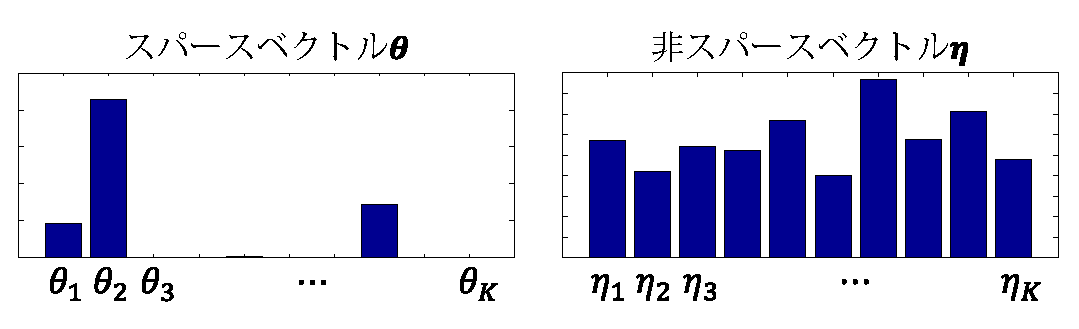
\includegraphics[width=.93\linewidth]{sections/music/sparse}
\caption{$K$次元のスパースベクトル$\bm\theta$と非スパースベクトル$\bm\eta$.
各ベクトルは各次元$k \ (1 \le k \le K)$に対して
$\theta_k \sim \mbox{Gamma}(0.1, 0.1)$,$\eta_k \sim \mbox{Gamma}(10, 10)$としてランダムに生成.
ただし,$\mathbb{E}[\theta_k] = \mathbb{E}[\eta_k] = 1$であることに注意.}
\label{fig:sparse}
\end{figure}

\begin{figure}[t]
\centering
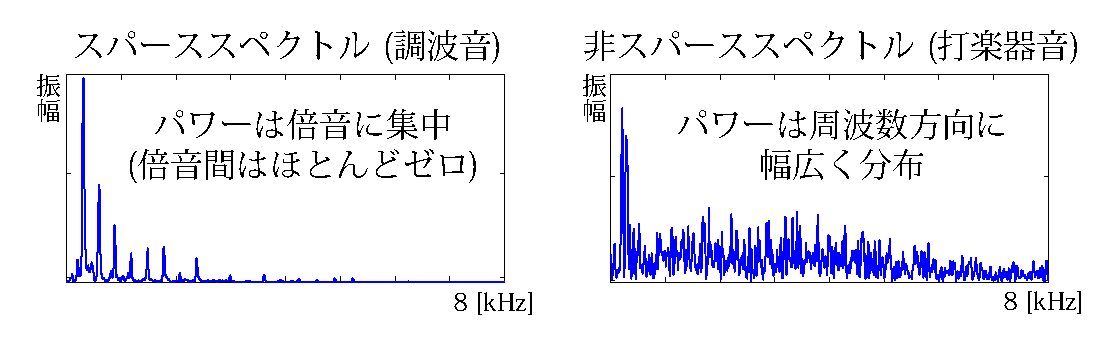
\includegraphics[width=.99\linewidth]{sections/music/sparse_spec}
\caption{調波構造を持つ楽器音(ピアノ)のパワースペクトルと
調波構造を持たない打楽器音(スネアドラム)のパワースペクトル.}
\label{fig:sparse_spec}
\end{figure}

ベクトルや行列がスパースであるとは,
ほとんどの要素がゼロをとる状態を指します(\reffig{fig:sparse}).
一見複雑に思える音楽音響信号も,
高々有限個の楽器音が重なりあってできています.
例えば,あるピアノ曲を考えてみると,
楽曲中に出現する音高は音域や調に依存することから,
ピアノの持つ88種類の音高(鍵盤の個数)の使われやすさに大きな偏りがあります.
また,音楽音響信号の構成要素そのものにもスパース性が存在します.
例えば,調波構造を持つ楽器音は,
倍音周波数付近にパワーが集中しており,
倍音間にはほとんどパワーが存在しません(\reffig{fig:sparse_spec}).
一方,バスドラムやスネアドラムのように,
明確な音高を持たない打楽器音は,周波数方向に幅広くパワーが分布しており,
スパースではありません.
\reffig{fig:sparse}に示すように,適切な確率分布を用いれば,
スパース性を表現することができます.

\subsection{低ランク性}

\begin{figure}[t]
\centering
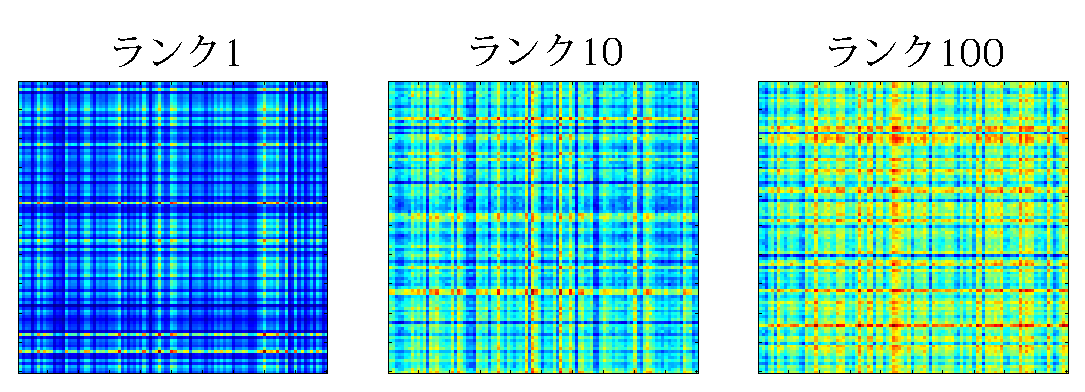
\includegraphics[width=.99\linewidth]{sections/music/low_rank_matrices}
\caption{ランク$K=1,10,100$の行列の例.
各行列$\bm{X}$は,$A_{nk} \sim \mbox{Gamma}(10,10)$および$B_{km} \sim \mbox{Gamma}(10,10)$として
行列$\bm{A} \in \mathbb{R}^{N \times K}$および
$\bm{B} \in \mathbb{R}^{K \times M}$をランダムに生成したあと,$\bm{X}=\bm{A}\bm{B}$として計算.}
\label{fig:low_rank_matrices}
\end{figure}

ある行列$\bm{X} \in \mathbb{R}^{N \times M}$が低ランクであるとは,
$K \ll M, N$として,
\begin{align}
\bm{X} = \bm{A}\bm{B}
\end{align}
となるような
行列$\bm{A} \in \mathbb{R}^{N \times K}$および
$\bm{B} \in \mathbb{R}^{K \times M}$が存在することをいいます.
ここで,$K$はランク(階数)と呼ばれ,
もとの行列$\bm{X}$の行数$M$や列数$N$よりはるかに小さい値をとります.
究極的には,$K=1$である場合に$\bm{X}$はランク1の行列となり,
$\bm{X} = \bm{a}\bm{b}^T$となるようなベクトル$\bm{a} \in \mathbb{R}^{N}$および
$\bm{B} \in \mathbb{R}^{M}$の直積で表現されます.

\begin{figure}[t]
\centering
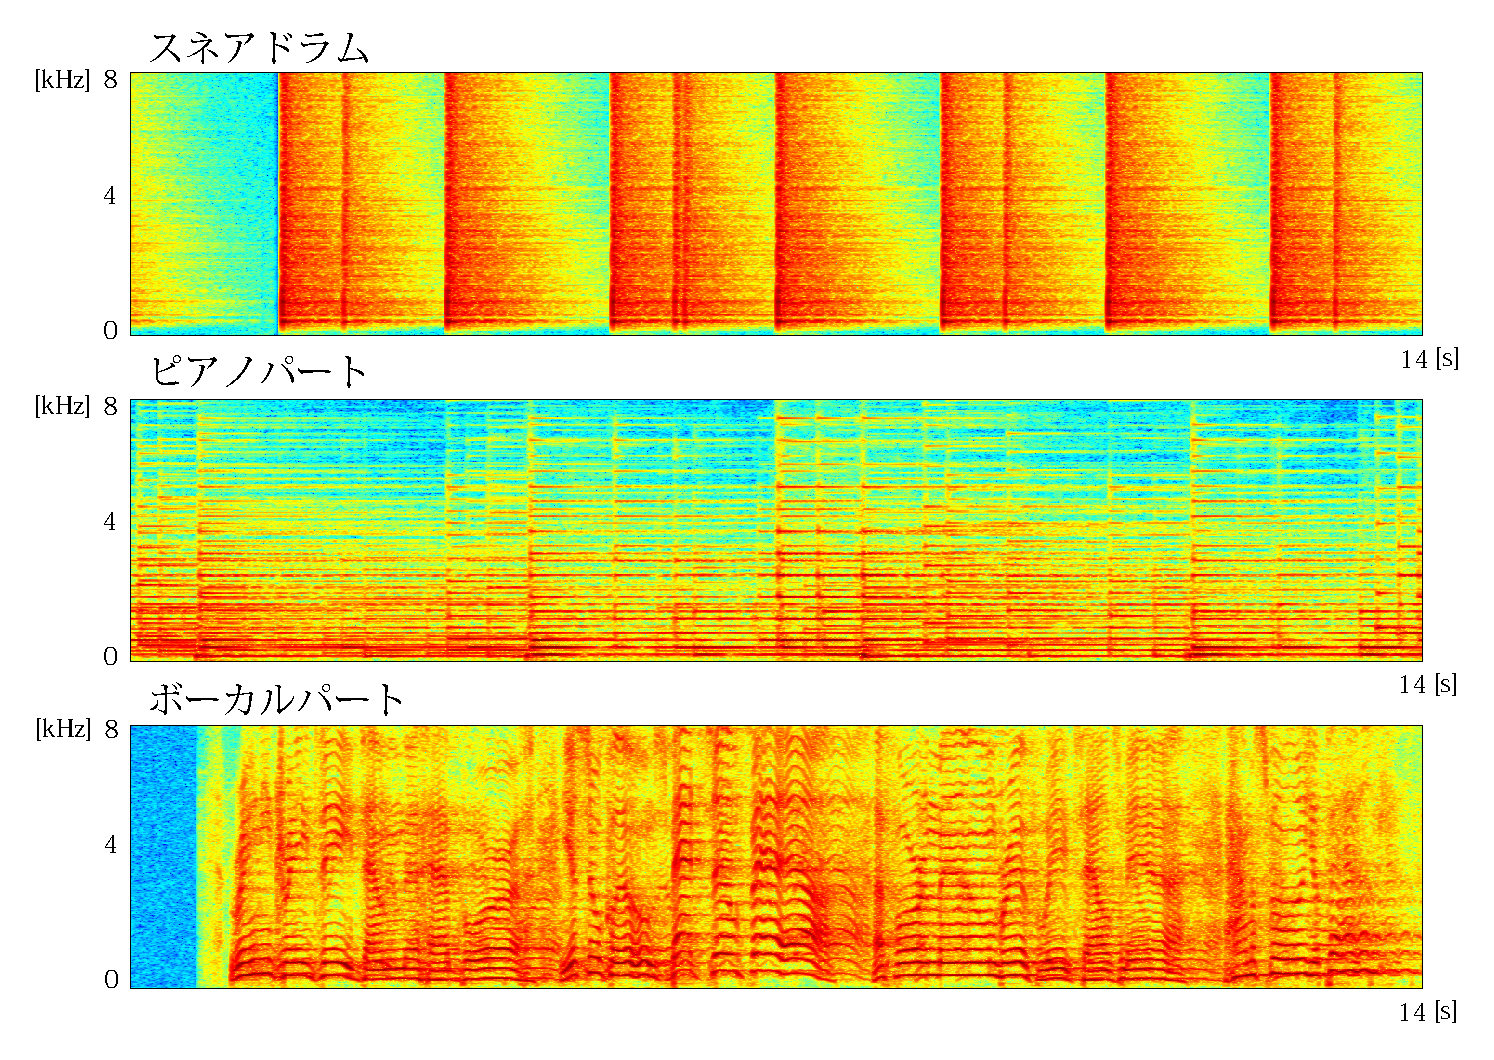
\includegraphics[width=.99\linewidth]{sections/music/low_rank_spectrograms}
\caption{スネアドラム,ピアノパート,ボーカルパートのパワースペクトログラム.
これらをそれぞれ行列とみなしたときに,この順番にランクが増加すると考えられる.
研究コミュニティベースの音源分離コンテストSiSEC 2008\cite{vincent:sisec:2008}において配布されている
開発用データに含まれる楽曲``bearlin roads''を利用.}
\label{fig:low_rank_spectrograms}
\end{figure}

低ランクの行列を可視化してみると,
布地の織り目のような縦横の模様があることに気づきます(\reffig{fig:low_rank_matrices}).
特にランク1の場合,行列を任意の場所で縦方向にスライスしてみると,
抜き出されるベクトルの全体的な形状は一定であり,そのスケールのみが変化することになります
(場所ごとに直径が変化する金太郎あめを想像してください).
行列を任意の場所で横方向にスライスする場合も同じことです.

実際の楽器音のスペクトログラムも,同様の縦横の模様を持っています(\reffig{fig:low_rank_matrices}).
特に,バスドラムやスネアドラムといった打楽器音は,
同じ形状のパワースペクトルが何度も繰り返し出現し,
各発音時刻の後では,パワースペクトルの形状が保たれたまま
音量が徐々に減衰していく現象がみられることから,
低ランクな行列(理想的にはランク1の行列)で近似することはある程度妥当であると考えられます.
ピアノパートは複数の音高の重畳で成り立っているため,
ランク1の行列で近似することは困難なものの,
やはり低ランク構造を持ちそうなことが分かります.
一方,ボーカルパートは,時間方向・周波数方向にパワースペクトルが複雑に変化しているため,
低ランクの行列とはみなすことは困難です.


\subsection{音源分離への応用}
\label{sec:nmf_separation}

NMFでは,基底ベクトル$\bm{w}_k$及び
アクティベーションベクトル$\bm{h}_k$がスパースになりやすい.
一方,同様の行列分解形式$\bm{X} = \bm{W}\bm{H}$を持つ
主成分分析 (Principal Component Analysis: PCA) では,
行列要素は負値をとることが許されている.
従って,\refeq{eqn:x_wh_elem}のように入力を基底の線形和で表現する際に,
基底の加減算による細かな調節が可能となる.
一方,NMFでは,基底の加算しか許されず,
いったんアクティベートされた基底の影響を打ち消すことはできない.
そのため,各基底$\bm{w}_k$が$\bm{x}_n$中の局所的な「パーツ」に対応し,
少数の基底で$\bm{x}_n$を表現する方が都合が良い.
NMFは当初,顔画像(ピクセル値ベクトル)の集合に対して適用され,
目・鼻・口といった顔のパーツ画像に対応する基底ベクトルが得られることが分かった.
このようなパーツに基づく分解表現は,音楽音響信号の分解と相性が良い.
なぜなら,調波音のスペクトルは周波数軸上でスパースであり,
混合音スペクトルは局所的な周波数帯域上のパーツの組み合わせとみなせるからである.

観測信号の複素スペクトログラムを
$\tilde{\bm{X}} = [\tilde{\bm{x}}_1,\cdots,\tilde{\bm{x}}_N] \in \mathbb{C}^{M \times N}$,
$k$番目の音源信号の複素スペクトログラムを
$\tilde{\bm{X}}_k = [\tilde{\bm{x}}_{k1},\cdots,\tilde{\bm{x}}_{kN}] \in \mathbb{C}^{M \times N}$とする.
$M$は周波数ビン数,$N$はフレーム数である.
観測した混合音が$K$個の音源信号の瞬時混合であると仮定すると,以下が成立する.
\begin{align}
 \tilde{\bm{X}} = \sum_{k=1}^{K} \tilde{\bm{X}}_{k}
 \ 
 \left(
 \tilde{\bm{x}}_n = \sum_{k=1}^{K} \tilde{\bm{x}}_{kn}
 \right)
 \label{eqn:s}
\end{align}

観測変数$\tilde{\bm{X}}$を潜在変数$\tilde{\bm{X}}_k$に分解する問題は不良設定であるので,
$\tilde{\bm{X}}_k$に対応する
パワースペクトログラム$\bm{X}_k = [\bm{x}_{k1},\cdots,\bm{x}_{kN}] 
\in \mathbb{R}_+^{M \times N}$ $(x_{knm} = |\tilde{x}_{knm}|^2)$は,
ランク1行列$\bm{Y}_k = [\bm{y}_{k1},\cdots,\bm{y}_{kN}] \in \mathbb{R}_+^{M \times N}$で
近似する(\reffig{fig:nmf}).
\begin{align}
 \bm{X}_k \approx \bm{w}_k \bm{h}_k^T \overset{\mbox{\tiny def}}{=} \bm{Y}_k
 \label{eqn:rank1}
\end{align}
すなわち,$\bm{Y}_k$の任意のフレーム$n$におけるパワースペクトル$\bm{y}_{kn}$は
基底スペクトル$\bm{w}_k \in \mathbb{R}^{M}$を
重み$h_{kn}$でスケーリングするだけで得られるという仮定をおいた($\bm{y}_{kn} = h_{kn} \bm{w}_k$).
%本来,調波構造中の倍音の相対強度は時変であるが,
%実際のスペクトル$\bm{X}_k$に対する近似モデルとしては有効に機能する.

\begin{figure}[t]
\centering
\includegraphics[width=.99\linewidth]{sections/music/nmf}
\caption{パワースペクトログラムに対する
ISダイバージェンスに基づく非負値行列分解 (IS-NMF) の適用結果.}
\label{fig:nmf}
\end{figure}

まず,潜在変数$\tilde{\bm{x}}_{kn}$が
$\bm{y}_{kn}$で定まる対角共分散行列を持つ複素ガウス分布に従うことを仮定する.
\begin{align}
 \tilde{\bm{x}}_{kn} \sim \mathcal{N}_c(\bm{0}, \mbox{diag}(\bm{y}_{kn}))
 \label{eqn:is_s_k_p}
\end{align}
ただし,$\mbox{diag}(\bm\eta)$はベクトル$\bm\eta$を対角成分に持つ対角行列を表す.
\refeq{eqn:s}に着目すると,
複素ガウス分布の再生性から
\begin{align}
 \tilde{\bm{x}}_n \sim \mathcal{N}_c(\bm{0}, \mbox{diag}(\bm{y}_n))
  \label{eqn:is_s_p}
\end{align}
を得る.ただし,$\bm{y}_n = \sum_k \bm{y}_{kn}$である.
従って,$x_{nm}=|\tilde{x}_{nm}|^2$は指数分布に従うことが分かる.
\begin{align}
 x_{nm} \sim \mbox{Exponential}(y_{nm})
 \label{eqn:is_p}
\end{align}
ここで,\refeq{eqn:is_s_p}の対数をとって符号反転させると,
\refeq{eqn:nmf_is}と定数項を除いて等しい.
従って,\refeq{eqn:is_s_p}の最大化(最尤推定)は
\refeq{eqn:nmf_is}の最小化と等価であり,
IS-NMFの適用が適切であると分かる.

最終的に,\refeq{eqn:is_s_k_p}及び\refeq{eqn:is_s_p}に着目すると,
$\tilde{\bm{x}}_n$が与えられたときの
$\tilde{\bm{x}}_{kn}$の事後分布は複素ガウス分布になることが分かり,
その平均と分散は
\begin{align}
 &
 \mathbb{E}[\tilde{\bm{x}}_{kn}|\tilde{\bm{x}}_{n}] 
 = \mbox{diag}(\bm{y}_{kn}) \mbox{diag}(\bm{y}_n)^{-1} \tilde{\bm{x}}_{n}
 \label{eqn:s_exp}
 \\
 &
 \mathbb{V}[\tilde{\bm{x}}_{kn}|\tilde{\bm{x}}_{n}] 
 = \mbox{diag}(\bm{y}_{kn}) 
 \nonumber\\
 & \ \ \ \ \
 - \mbox{diag}(\bm{y}_{kn}) \mbox{diag}(\bm{y}_n)^{-1} \mbox{diag}(\bm{y}_{kn})
 \label{eqn:s_var}
\end{align}
で与えられる.
この処理はウィナーフィルタリングと呼ばれ,
$\tilde{\bm{X}}_k$の位相は$\tilde{\bm{X}}$の位相と同一であるという仮定が置かれている.
最後に,逆フーリエ変換を用いて,
$\mathbb{E}[\tilde{\bm{X}}_k|\tilde{\bm{X}}]$から
$k$番目の音源信号を復元することができる.

\begin{figure}[t]
\centering
\includegraphics[width=.98\linewidth]{sections/music/nmf_samples}
\caption{異なる基底数$K$に対するIS-NMFの結果.}
\label{fig:nmf_samples}
\end{figure}

基底数$K$を変化させながらIS-NMFを適用した結果を\reffig{fig:nmf_samples}に示す.
$K$が小さすぎると近似が荒く,
$K$を大きくしすぎると物理的な意味を持たない極めて局所的な基底ばかりになる.
このことから,基底数$K$を適切に定める重要性が分かる.

実際には,性質の良くない局所解に陥りやすいIS-NMFの代わりに
KL-NMFが利用される場合が多い.
このとき,$\bm{X}$や$\bm{X}_k$は
振幅スペクトログラムとするのが一般的である($x_{knm} = |\tilde{x}_{knm}|$).

まず,潜在変数$x_{knm}$が$y_{knm}$で定まるポアソン分布に従うことを仮定する.
\begin{align}
 x_{knm} \sim \mbox{Poisson}(y_{knm})
 \label{eqn:kl_s_k_p}
\end{align}
ここで,複数の音源信号の重畳における振幅スペクトルの加法性を仮定すると
(実際には成立しないことに注意),ポアソン分布の再生性から
\begin{align}
 x_{nm} \sim \mbox{Poisson}(y_{nm})
 \label{eqn:kl_s_p}
\end{align}
を得る.
ここで,\refeq{eqn:kl_s_p}の対数をとって符号反転させると,
\refeq{eqn:nmf_kl}と定数項を除いて等しい.
従って,\refeq{eqn:kl_s_p}の最大化(最尤推定)は
\refeq{eqn:nmf_kl}の最小化と等価である.


\subsection{音源分離への応用}
\label{sec:mf}

\refeq{eqn:s}を満たすように,
$\tilde{\bm{x}}_n$を
$\{\tilde{\bm{x}}_{kn}\}_{k=1}^K$の和に分解したい.
まず,潜在変数$\tilde{\bm{x}}_{kn}$が
共分散行列$\bm{Y}_{kn}$を持つ複素ガウス分布に従うことを仮定する.
\begin{align}
 \tilde{\bm{x}}_{kn} \sim \mathcal{N}_c(\bm{0}, \bm{Y}_{kn})
 \label{eqn:ld_s_k_p}
\end{align}
ここで,\refeq{eqn:is_s_k_p}のように共分散行列を対角行列に限定しないことで,
周波数ビン間の相関を考慮している.
\refeq{eqn:s}と複素ガウス分布の再生性から
\begin{align}
 \tilde{\bm{x}}_n \sim \mathcal{N}_c(\bm{0}, \bm{Y}_n)
  \label{eqn:ld_s_p}
\end{align}
を得る.ただし,$\bm{Y}_n = \sum_k \bm{Y}_{kn}$である.
ここで,\refeq{eqn:ld_s_p}の対数をとって符号反転させると,
\refeq{eqn:psdtf_ld}と定数項を除いて等しい.
従って,\refeq{eqn:ld_s_p}の最大化は
\refeq{eqn:psdtf_ld}の最小化と等価であり,
LD-PSDTFを用いて$\bm{Y}_n$や$\bm{Y}_{kn}$を求めることができる.

最終的に,\refeq{eqn:ld_s_k_p}, (\ref{eqn:ld_s_p})から,
$\tilde{\bm{x}}_n$が与えられたときの
$\tilde{\bm{x}}_{kn}$の事後分布は複素ガウス分布になることが分かり,
その平均と分散は次式となる.
\begin{align}
 &\!\!\!\!\!\!\!\!
 \mathbb{E}[\tilde{\bm{x}}_{kn}|\tilde{\bm{x}}_n] 
 =
 \bm{Y}_{kn} \bm{Y}_n^{-1} \tilde{\bm{x}}_n
 \label{eqn:e_xn}
 \\
 &\!\!\!\!\!\!\!\!
 \mathbb{V}[\tilde{\bm{x}}_{kn}|\tilde{\bm{x}}_n] 
 =  
 \bm{Y}_{kn} - \bm{Y}_{kn} \bm{Y}_n^{-1} \bm{Y}_{kn}
 \label{eqn:v_xn}
\end{align}
ここで,\refeq{eqn:s_exp}とは異なり,
$\tilde{\bm{X}}_k$の位相は$\tilde{\bm{X}}$の位相とは異なる点に注意する.
IS-NMFのように各周波数ビン$n,m$ごとではなく,
各フレーム$n$ごとに一挙に分離を行うことで,
周波数ビン間の相関を考慮しながら高品質な分離が可能となる.

\begin{algorithm}[t]
\caption{LD-PSDTFの最尤推定}         
\label{ld-psdtf-ml}
\begin{algorithmic}[1]
\Require テンソル$\bm{X} \in \mathbb{C}^{M \times M \times N}$, 基底数$K$
\State 基底テンソル$\bm{W} \in \mathbb{C}^{M \times M \times K}$をランダムに初期化
\State 非負値行列$\bm{H} \in \mathbb{R}_+^{M \times K}$をランダムに初期化
\While{not converged}
\State $\bm{P}_k = \sum_{n=1}^{N} h_{kn} \bm{Y}_n^{-1}$
\State $\bm{Q}_k = \sum_{n=1}^{N} h_{kn} \bm{Y}_n^{-1} \bm{X}_n \bm{Y}_n^{-1}$
\State コレスキー分解$\bm{Q}_k = \bm{L}_k \bm{L}_k^T$
\State $\bm{W}_k 
 \gets
 \bm{W}_k \bm{L}_k(\bm{L}_k^T \bm{W}_k \bm{P}_k \bm{W}_k \bm{L}_k)^{-\frac{1}{2}}\bm{L}_k^T \bm{W}_k$
\State  $h_{kn} \gets h_{kn}
 \left(\frac{\mbox{tr}\!\left(\bm{Y}_n^{-1} \bm{W}_k \bm{Y}_n^{-1} \bm{X}_n\right)}
            {\mbox{tr}\!\left(\bm{Y}_n^{-1} \bm{W}_k \right)}\right)^{\frac{1}{2}}$
\EndWhile\\
{\bf Return} 基底テンソル$\bm{W}$,非負値行列$\bm{H}$
\end{algorithmic}
\end{algorithm}

\subsection{確率モデルの最尤推定としての定式化}

文献\cite{yoshii:ismir:2013,yoshii:icml:2013}において,
NMFと同様にガンマ過程を用いて基底数を$K \rightarrow \infty$とした
ノンパラメトリックベイズモデルが提案されている.
今後の課題として,vN-PSDTFに対する乗法更新則の導出や計算量の削減が挙げられる.



\section{楽器パートの分離}

\subsection{歌声・伴奏音の分離}

最後に,スパース性に基づいて音楽音響信号を楽器種別に分離する技術を紹介する.
ロバスト主成分分析 (RPCA) は,入力行列$\bm{X}$を
低ランク行列$\bm{L}$とスパース行列$\bm{S}$の和に分解する.
具体的には,$\bm{X} = \bm{L} + \bm{S}$を満たすという制約のもとで,
以下で定義される最適化問題を解く.
\begin{align}
 \mbox{minimize} \ \|\bm{L}\|_* +\lambda \|\bm{S}\|_1
\end{align}
ここで,$\|\cdot\|_*$,$\|\cdot\|_1$はそれぞれ核ノルム,L1ノルムである.
厳密ではないが拡張ラグランジュ法に基づく効率的な解法を{\bf Algorithm \ref{rpca}}に示す.
\refsec{sec:introduction}で議論したとおり,
混合音スペクトログラムを$\bm{X}$として与えると,
伴奏音スペクトログラム$\bm{L}$と歌声スペクトログラム$\bm{S}$が得られる.
また,メディアンフィルタを時間方向・周波数方向に適用することで
調波音・打楽器音を分離すること (Harmonic/Percussive Source Separation: HPSS) 
も可能である\cite{fitzgerald:dafx:2010}.
これらの技術による分離結果を\reffig{fig:separation}に示す.

\begin{algorithm}[t]
\caption{Inexact ALMに基づくRPCA}
\label{rpca}                          
\begin{algorithmic}[1]
\Require 入力行列$\bm{X} \in \mathbb{R}^{M \times N}$,重み係数$\lambda$
\State 初期化:$\bm{Y} = \bm{X} / \max(\|\bm{X}\|_2, \lambda^{-1}\|\bm{X}\|_\infty) \in \mathbb{R}^{M \times N}$
\State 初期化:$\bm{S} = \bm{0} \in \mathbb{R}^{M \times N}$
\State 初期化:$\mu > 0$ ({\it e.g.}, $\mu = 1.25 / \|\bm{X}\|_2 $)
\State 初期化:$\rho > 1$ ({\it e.g.}, $\rho = 1.5$)
\While{not converged}
\State $[\bm{U}, \bm\Sigma, \bm{V}] = \mbox{SVD}(\bm{X} - \bm{S} + \mu^{-1} \bm{Y})$
\State $\bm{L} \gets \bm{U} \mathcal{F}_{\mu^{-1}}(\bm\Sigma) \bm{V}^T$
\State $\bm{S} \gets \mathcal{F}_{\lambda\mu^{-1}}(\bm{X} - \bm{L} + \mu^{-1} \bm{Y})$
\State $\bm{Y} \gets \bm{Y} + \mu (\bm{X} - \bm{L} - \bm{S})$
%\If {$\mu\|\bm{S} - \bm{S}_{\mbox{\scriptsize old}}\|_F/\|\bm{X}\|_F < \epsilon$}
\State $\mu \gets \rho \mu$
%\EndIf
\EndWhile
\\
{\bf Return} 低ランク行列$\bm{L}$,
スパース行列$\bm{S} \in \mathbb{R}^{M \times N}$
\end{algorithmic}
*$\mathcal{F}_\epsilon[x] 
= x - \epsilon \ (\mbox{if} \ x > \epsilon), 
  x + \epsilon \ (\mbox{if} \ x < -\epsilon), 
  0 \ (\mbox{otherwise})$
\end{algorithm}

\subsection{調波音・非調和音の分離}

HPSSのいくつかの手法を紹介.

\subsection{音色に基づく分離}

ソースフィルタモデル

\section{おわりに}

本稿では,スパース性に基づく音楽音響信号分解技術として,
非負値行列分解 (NMF),半正定値テンソル分解 (PSDTF),
ロバスト主成分分析 (RPCA),調波・打楽器分離音 (HPSS) を紹介した.
これらは音声情報処理分野の影響を受けながら,
音楽情報処理分野で独自の発展を遂げている.
例えば,NMF(音響モデル)はソース・フィルタ型の楽器音モデルや,
楽譜の生成モデル(言語モデル)と統合する試みが進んでいる.
本稿が読者の理解の一助になれば幸いである.

\begin{figure}[t]
\centering
\includegraphics[width=.99\linewidth]{sections/music/separation}
\caption{音楽音響信号に対するRPCA・HPSSの適用結果.}
\label{fig:separation}
\end{figure}

%% 文献
%\bibliographystyle{unsrt}
%\bibliography{yoshii,yoshii-nmf,yoshii-lpc}

\begin{thebibliography}{10}

\bibitem{lee:nature:1999}
D. D. Lee and H. S. Seung, 
\newblock ``Learning the parts of objects by non-negative matrix factorization,'' 
\newblock {\em Nature}, {\bf 401}, 788--791 (1999).

\bibitem{fevotte:neco:2009}
C.‾{F\'{e}votte}, N.‾Bertin, and J.-L. Durrieu,
\newblock ``Nonnegative matrix factorization with the {I}takura-{S}aito
  divergence: {W}ith application to music analysis,''
\newblock {\em Neural Computation}, {\bf 21(3)}, 793--830 (2009).

\bibitem{hoffman:icml:2010}
M.‾Hoffman, D.‾Blei, and P.‾Cook,
\newblock ``{B}ayesian nonparametric matrix factorization for recorded music,''
\newblock {\em ICML}, 439--446 (2010).

\bibitem{yoshii:icml:2013}
K.‾Yoshii, R.‾Tomioka, D.‾Mochihashi, and M.‾Goto,
\newblock ``Infinite positive semidefinite tensor factorization for source
  separation of mixture signals,''
\newblock {\em ICML}, 576--584 (2013).

\bibitem{yoshii:ismir:2013}
K.‾Yoshii, R.‾Tomioka, D.‾Mochihashi, and M.‾Goto,
\newblock ``Beyond NMF: Time-domain audio source separation without phase
  reconstruction,''
\newblock {\em ISMIR}, 369--374 (2013).

\bibitem{lin:mp:2010}
Z.‾Lin, M.‾Chen, and Y.‾Ma,
\newblock ``The augmented {L}agrange multiplier method for exact recovery of
  corrupted low-rank matrices,''
\newblock {\em Math. Prog.} (2010).

\bibitem{fitzgerald:dafx:2010}
D.‾FitzGerald,
\newblock ``Harmonic/percussive separation using median filtering,''
\newblock {\em DAFx} (2010).

\bibitem{smaragdis:waspaa:2003}
P.‾Smaragdis and J.‾C. Brown,
\newblock ``Non-negative matrix factorization for polyphonic music transcription,''
\newblock {\em WASPAA}, 177--180 (2003).

\bibitem{kameoka:asjj:2012}
亀岡弘和,
\newblock ``非負値行列因子分解の音響信号処理への応用,''
\newblock {\em 日本音響学会誌}, 68(11), 559--565 (2012).

\bibitem{sawada:ieee:2013}
H.‾Sawada, H.‾Kameoka, S.‾Araki, and N.‾Ueda,
\newblock ``Multichannel extensions of non-negative matrix factorization with complex-valued data,''
\newblock {\em IEEE Trans. TASLP}, {\bf 21(5)}, 971--982 (2013).

\bibitem{kulis:jmlr:2009}
B.‾Kulis, M.‾Sustik, and I.‾Dhillon,
\newblock ``Low-rank kernel learning with {B}regman matrix divergences,''
\newblock {\em JMLR}, {\bf 10}, 341--376 (2009).

\end{thebibliography}



%\section{ソース・フィルタ分解}

%\section{調波音・打楽器音分離}

%\section{時間領域分解}

%また,構成要素のスパース性に着目することで,
%市販CDのように複雑な音楽音響信号に対しても,
%歌声・伴奏音を分離したり,調波音・打楽器音を分離することができる.
%音色や音高のバリエーションに富む歌声を含む音楽音響信号は,
%NMFのように少数の基底の線形和で表現することは難しい.
%一方,ロバスト主成分分析 (Robust Principal Component Analysis: RPCA)\cite{lin:mp:2010}
%を用いると,線形和で表現可能な低ランクな伴奏音成分と,
%外れ値とみなせるスパースな歌声成分とに分離可能である.
%また,時間・周波数平面において,
%調波構造を持つ楽器音は周波数方向にスパースであり,
%減衰が早い打楽器音は時間方向にスパースである.
%従って,周波数・時間方向にそれぞれメディアンフィルタを適用すれば,
%外れ値となる調波音・打楽器音をそれぞれ抑制することができる\cite{fitzgerald:dafx:2010}.


\chapter{マイクロホンアレイ音響信号解析}

\begin{leadbox}
本章では,マイクロホンアレイ音響信号解析技術について説明します.
\end{leadbox}

\section{音源定位}

\section{音源分離}

\section{残響除去}

\section{音源定位・音源分離・残響除去の統合モデル}


%\appendix %%%% 付録

%本稿中で使用した確率密度関数を掲載しておく.
%\begin{align}
%&\mbox{Gamma}(x|a,b) = \frac{b^a}{\Gamma(a)} x^{a - 1} \exp(- bx)
%\\
%&\mbox{Exponential}(x|\lambda) = \mbox{Gamma}(x|1,1/\lambda)
%\end{align}
%\begin{align}
%&\mbox{Poisson}(x|\lambda) = \frac{\lambda^x}{x!}\exp(-\lambda)
%\\
%&\mathcal{N}_c(\bm{x}|\bm{0},\bm\Sigma) 
%= \frac{1}{\pi^M |\bm\Sigma|} \exp(- \bm{x}^H \bm\Sigma^{-1} \bm{x})
%\end{align}

%
%\addcontentsline{toc}{index}{索引}
%\printindex
\backmatter
%
\end{document}
